%!TEX encoding = UTF-8 Unicode
\documentclass[a4paper,12pt]{book}
%\usepackage[top=3.5cm,right=3cm,bottom=4cm,left=3cm]{geometry}  
\usepackage{amsmath}
 \usepackage[marginal,stable,bottom]{footmisc}     % for footnotes: marginal --> the same margins as text, 
                                                                                  %                       stable--> ?
                                                                                  %                       bottom --> starting the footnotes at a fixed place at the bottom of the page.
 
\usepackage{perpage}                                             % for footnotes: starting from 1 perpage
\MakePerPage{footnote}
\usepackage{cite}                                                     % for collecting citations: [1,2,3,4] --> [1-4]
\usepackage{setspace}                                            % for switching between double/single space in document
\allowdisplaybreaks                                                    % breaking the lines&pages when needed for the style.
\usepackage{parskip}                                               % ? 

%\relpenalty=9999                                            % show the neccessity of breaks for lines, changing the number to 10000 cause no break in lines.
%\binoppenalty=9999
%%%%%%%%%% by me
\usepackage{textcomp}
\usepackage{amssymb}
%%%%%%%%%%
\usepackage{xecolour}
\usepackage{url}
\usepackage{mathtools}
\usepackage{amsmath}
\usepackage{makeidx}
\usepackage{verbatim}
\usepackage[colorlinks,linkcolor=blue,citecolor=blue]{hyperref}
\usepackage{graphicx}
\usepackage{ifthen}

 \parindent0pt


\makeatletter
\pdfstringdefDisableCommands{%
\let\lr\@firstofone
}
\makeatother
% ----------------------------------------------------------------------------
\usepackage{xepersian}

\usepackage[Lenny]{fncychap}

\settextfont[Scale=1.07]{XB Niloofar}
\setlatintextfont[Scale=1.05]{Times New Roman} 
\setdigitfont[Scale=1.05]{XB Niloofar} 
% \setdigitfont[Scale=1.05]{Yas} 
% قلم برای اعداد به صورت فارسی با صفر توخالی، در صورتی که بخواهیم اعداد انگلیسی نوشته شوند این خط را غیر فعال می‌کنیم.


\defpersianfont\nastaliq[Scale=2.0]{IranNastaliq}
% قلم برای نوشتن تقدیم
\defpersianfont\nastaliqone[Scale=1.0]{IranNastaliq}
% قلم نستعلیق با سایز متناسب با متن در صورت نیاز
\defpersianfont\anotherfont[Scale=1.2]{XP Ziba}
% قلم برای نوشتن تشکر (قلم فانتزی)
\newenvironment{fantezi}
{\anotherfont }


\makeindex


\def\beginto{
\newpage
\begin{RTL}
\begin{Huge}
\nastaliq

\begin{center}
\vspace*{0.15cm}
}

\def\endto{
~
\end{center}
\end{Huge}
\end{RTL}
}

\def\beginthanks{
\newpage

{\centering\Huge{\nastaliqone{
تشکر وقدردانی ~\\
~\\}}}
}

\def\endthanks{
~
}

\def\thanks{
\beginthanks
\input{thanks}
\endthanks
}

\def\startpage{
\newpage
\vspace*{3cm}
\begin{center}

\includegraphics[width=12cm]{besm}
\end{center}
}
\makeatletter
\def\@makechapterhead#1{%
  \vspace*{50\p@}%
  {\parindent \z@ \centering\normalfont
    \ifnum \c@secnumdepth >\m@ne
      \if@mainmatter
        \huge\bfseries \@chapapp\space \tartibi{chapter} 
        \par\nobreak
        \vskip 20\p@
      \fi
    \fi
    \interlinepenalty\@M
    \Huge \bfseries #1\par\nobreak
    \vskip 40\p@
  }}
\def\@makeschapterhead#1{%
  \vspace*{50\p@}%
  {\parindent \z@ \centering
    \normalfont
    \interlinepenalty\@M
    \Huge \bfseries  #1\par\nobreak
    \vskip 40\p@
  }}
\makeatother



\renewcommand\bibname{مراجع}
\def\contentsname{فهرست}

% some extra diffinitions %%%%%%%%%%%%%%%%%
%%%%%%%%%%%%%%%%%%%%%%%%%%%%%

\def\bea{\begin{eqnarray}}
\def\eea{\end{eqnarray}}

\def\ba{\begin{array}}
\def\ea{\end{array}}

\def\ni{\noindent}
\def\nn{\nonumber}

\def\bc{\begin{center}}
\def\ec{\end{center}}

\usepackage{graphicx}
\usepackage[top=3cm,right=2.5cm,bottom=3cm,left=2.5cm]{geometry}  
\usepackage{fancyhdr}
\usepackage{amssymb} %for complicated latex symbols
\usepackage{amsmath}
\pagestyle{plain}
\usepackage{setspace}
\usepackage[colorlinks,linkcolor=blue,citecolor=blue,pagebackref=false]{hyperref}
\usepackage{xepersian}
\settextfont[Scale=1]{XB Niloofar}
\setlatintextfont[Scale=1]{Times New Roman}
\setdigitfont[Scale=1]{XB Niloofar}
\usepackage{cite}

\lhead{\thepage}
\chead{}
\cfoot{}
\renewcommand{\headrulewidth}{0.4pt}
\renewcommand{\footrulewidth}{0.4pt}

\fancypagestyle{fpstyle}{%
\fancyhead{} % get rid of headers
\renewcommand{\headrulewidth}{0pt} % and the line
}
\setlatintextfont[Scale=.9]{Times New Roman}
%\graphicspath{{Figs/}}

\newcommand{\fatitle}{بررسی چیدمان کروماتین درون هسته}
\newcommand{\faAuthor}{علی فرنودی}
\newcommand{\fasupervisor}{دکتر محمد رضا اجتهادی}
\newcommand{\fadate}{آبان 1396}
\newcommand{\falevel}{دکتری}
\newcommand{\fadepart}{دانشکده فیزیک}

%\newcommand{\entitle}{ DNA chains entanglement in confined geometries}
%\newcommand{\enAuthor}{Zahra Ahmadian}
%\newcommand{\ensupervisor}{Mohammad Reza Ejtehadi}
%\newcommand{\engdate}{August 2015}
%\newcommand{\enlevel}{Master of Science}
%\newcommand{\enDep}{Physics Department}

%\newcommand{\momtahenin}{دکتر سامان مقیمی عراقی }
%\newcommand{\momtahenou}{دکتر عباس  علی صابری}
\usepackage{perpage} %the perpage package
\usepackage{amsmath}
\MakePerPage{footnote} %the perpage package command



\begin{document}
%\onehalfspacing
\doublespacing
\cleardoublepage
\pagenumbering{roman} 

\begin{center}
\thispagestyle{empty}

\includegraphics{Figs/logo} \\
\begin{Large}
دانشگاه صنعتی شریف \\
\fadepart \\ [1cm]
رساله  \falevel \\

\end{Large}
\vskip 3cm
\large{عنوان}  \\ \textbf{\large{\fatitle}}
\vskip 2cm
\large{نگارنده:} \\ \Large{\faAuthor}
\vskip 2cm
\large{استاد راهنما:} \\ \Large{\fasupervisor}
\vskip 2cm
\large{\fadate}
\end{center}


\thispagestyle{empty}
\noindent
\vskip 7cm
\begin{center}

\includegraphics[scale=0.8]{Figs/besm.png}
\end{center}
\thispagestyle{empty}
\noindent
\centerline{\textbf{\large{چکیده}}} \\
در فصل اول این پژوهش مروری بر مطالعات اخیر افراد در مورد ساختار اسکلت سلولی و عوامل دخیل در انتقال نیرو در سلول‌های دارای هسته شده است. فیزیک رفتار مواد ویسکوالاستیک با جزئیات نیز بررسی شده‌. در ادامه‌ی این فصل برخی مطالعات منتخب معرفی شده‌ که در آن از مدل‌های ویسکوالاستیکی برای  مدل‌سازی نتایج آزمایشگاهی رفتار بخش‌های مختلف سلول استفاده شده‌است. در نهایت ساختار کروماتین در هسته‌ی سلول و ماتریس اتصالات کروماتین‌ها درون هسته نیز بررسی شده‌است. همچنین برخی از مدل‌هایی که در ۲-۳ سال گذشته برای توجیه این ساختار و ماتریس اتصالات انتشار یافته نیز مطالعه شده‌است. \\
در فصل دوم طرح پژوهشی توضیح داده شده و در فصل آخر منابع مورد استفاده نامبرده شده‌است.
\\
\\
\textbf{کلمات کلیدی:}
کروماتین، ماتریس اتصالات، ویسکوالاستیک، هسته سلول، شبیه‌سازی دینامیک ملکولی
\textit{}



\tableofcontents
\clearpage
\listoffigures

%path variables:
\def \Mempath {Chapters/Membrane}
\pagenumbering{arabic} 

\clearpage
\clearpage
\chapter{
\centering{
غشای زیستی
}
}
\setRL
\clearpage

\def \MemBio {\Mempath /MembraneBio}

\section{
چکیده
}
این فصل با مقدمه‌ای از نقش غشای زیستی در سلول شروع شده‌است (بخش
\ref{sec:memBioIntro}).
 سپس، مرور کوتاهی بر تارخچه‌ی تحقیقات انجام شده در جهت کشف و بررسی ساختار غشای سلول‌های زنده در قرن‌های ۱۹ و ۲۰ میلادی ارايه شده‌است (بخش
\ref{sec:memBioHistory}).
در ادامه، در مورد ساختار واحد‌های تشکیل دهنده‌ی غشا بحث شده (
\ref{sec:memBioSelfAssembily}
تا
\ref{sec:memBioFluidity})
 و در نهایت در مورد چیدمان غشای هسته یا بسته‌ی هسته توضیح داده شده‌است (بخش
\ref{sec:nuclearenvelope}).
 
 
\section{\label{sec:memBioIntro}
مقدمه
}
\setRL
%\pagenumbering{arabic} 


%\section{\label{sec:cellmembrane}
%غشای سلولی
%}
\section{
مقدمه
}
\begin{figure}[h]
\begin{center}
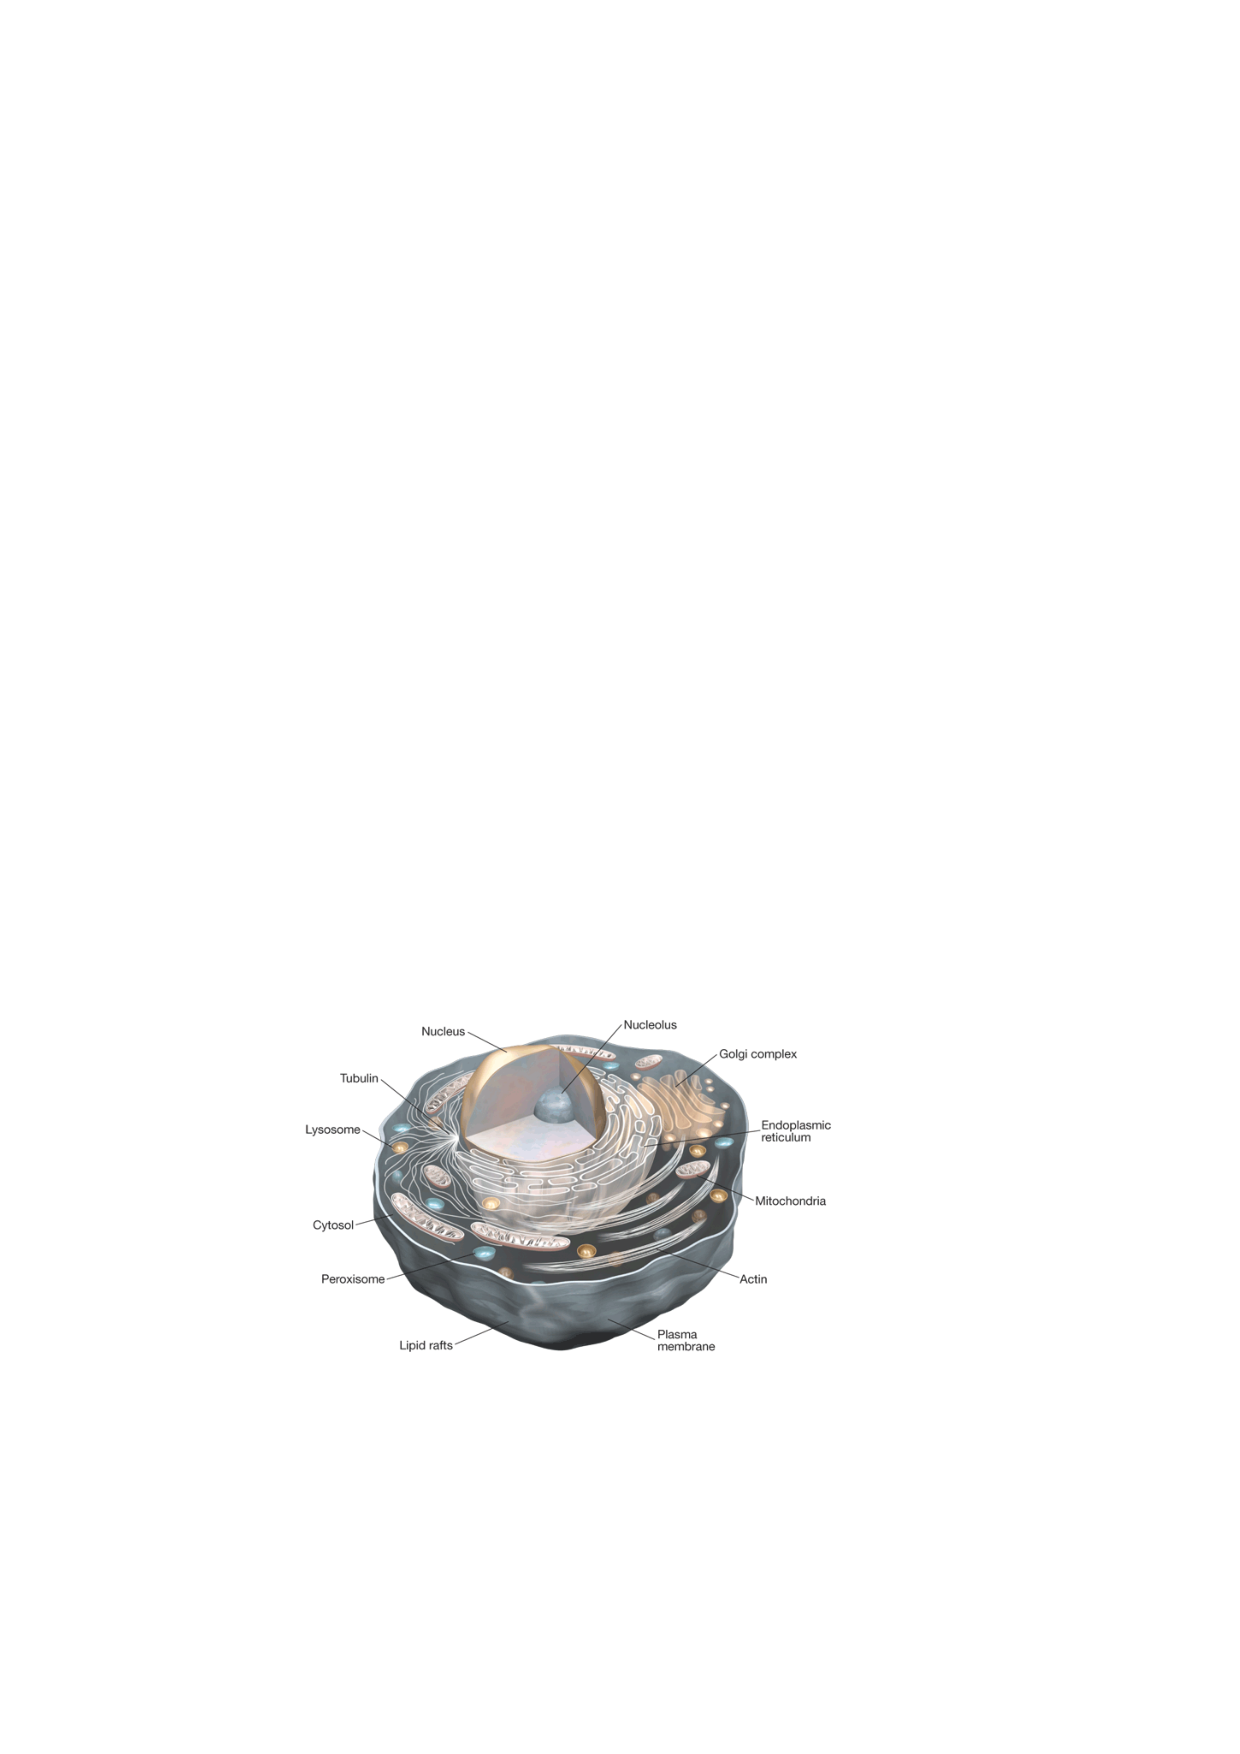
\includegraphics[width=6in]{\MemBio /Pics/CellParts}
\caption{
شکل طراحی شده از سلول پستانداران که غشا و اعضای سلول را نشان می‌دهد
\cite{CellParts}.
}
\label{fig:cellparts}
\end{center}
\end{figure}

مهم‌ترین نقش غشاهای زیستی ایجاد یک دیوار یا مانع برای مشخص کردن مرز داخل و خارج سلول است که نیاز اولیه‌ی وجود حیات به حساب می‌آید
\cite{Boyle2008Biology}.
 علاوه بر در-بر-گرفتنِ تمام اعضای یک سلول، در سلول‌های هسته‌دار، غشای هسته اورگان‌های خیلی مهم سلول را نیز در خود جا داده و محافظت می‌کند (شکل
\ref{fig:cellparts}). به عنوان مرز سلول با دینای خارج، غشا نقش مهمی در مدیریتِ نقل و انتقال مواد بین سلول و محیط پرامون دارد. درون غشا پروتئین‌ها، لیگاند‌ها
\LTRfootnote{ligand}،
و ملکول‌های درشت خیلی زیادی وجود دارد که در طیف‌ گسترده‌ای از فرآیندها نقش دارند. برای مثال غشا نقل و انتقال یون‌ها به درون و خارج سلول را از طریق کانال‌های پروتئینی مدیریت می‌کند
\cite{NEHER1976ProteinChannel}،
نسبت به تغییر فشار اُسمزی محیط واکنش نشان می‌دهد
\cite{Perozo2006Osmotic,Vasquez2009Osmotic,Haswell2011Osmotic}،
و همچنین در ساز و کار‌های بزرگ مقیاس مانند تقسیم سلولی، حرکت و جابجایی سلول، و چسبیدن به سطوح نقش دارد.


غشای سلول در خیلی از مسائل مهم پزشکی نیز مطرح می‌شود، مانند نقش آن در انتقال پالس الکتریکی در سلول‌های عصبی هنگام بیهوشی عمومی 
\cite{BioMemBook2007}.
همچنین بیشتر تلاش صنعت داروسازی طراحی داروی مناسب برای اتصال به پروتئین‌های روی سطح غشاست. تقریبا یک سوم پروتئین‌های دروی بدن در غشای سلول قرار دارند که  مورد هدف ۶۰ در صد از داروی‌های موجود در بازار هستند
\cite{DrugDelivery2007}.
 دانش یافته شده از مطالعه‌ی غشا در تکنولوژی‌های مدرن مانند بسته‌بندی و انتقال دارو
\cite{Torchilin2006Drugdelivery}،
ایجاد اتاقک‌های کوچک برای انجام واکنش‌های شیمیایی
\cite{Karlsson2001MemChamber}،
 و ساخت حس‌گرهای زیستی (ترکیب دستگاه‌های الکتریکی با غشا) کاربرد دارد
\cite{MemeElctronics2012}.


\section{\label{sec:memBioHistory}
تاریخچه کوتاه
}
\setRL
%\pagenumbering{arabic} 
\section{
تاریخچه کوتاه
}
حاصل زحمات افراد در قرن ۱۹ و ۲۰ میلادی در راستای پی بردن به ساز و کار واحد‌های سازنده‌ی موجودات زنده، ساخت تصویری با جزئیات زیاد از سلول‌های زنده است. در سال ۱۹۸۵ ارنست اُورتن\LTRfootnote{Ernest Overton}  
سلول‌های گیاهی را در محلول‌های مختلف (قند،‌ الکل، اتر، فنول، و اَسِتُن\LTRfootnote{sugar, alcohols, ether, phenol, and acetone}) قرار داد. مشاهدات وی نشان داد که (تحت اختلاف فشار اسمزی یکسان) محلول‌هایی مانند قند که در آب به راحتی حل می‌شوند نمی‌توانند وارد سلول شوند. در صورتی که محلول‌های دیگری که حل شونده‌ی خوبی در آب نیستند، می‌توانند وارد سلول شوند. او نتیجه گرفت که جنس مرز سلول با سیتوپلاسم درون آن متفاوت است و به احتمال زیاد از ملکول‌های چربی گون تشکیل شده است
\cite{overton1985}.

در سال ۱۹۱۷ اِروین لَنگموئر \LTRfootnote{Irving Langmuir}
 مقاله‌ای چاپ کرد که در آن روشی برای اندازه‌گیری فشار جانبی\LTRfootnote{lateral}
 غشا در سطح مقطع مشترک هوا و آب پیشنهاد داد
 \cite{Langmuir1917}.
 او با استفاده از روش خود نشان داد که غشا در این سطح مقطع مشترک یک تک لایه‌ی ملکول چرب تشکیل می‌دهد و مساحت هر ملکول را 
 $S_{lipid} = 0.7 nm^2$
 گزارش کرد. او همچنین در گزارش خود پیشنهاد داد که غشا از ملکول‌های دوزیست\LTRfootnote{Amphiphiles}
 تشکیل شده. ملکول‌های دوزیست به ملکول‌هایی گفته می‌شود که یک گروه سَر دو قطبی آب‌دوست و یک یا چند دُم هیدروکربنی آب‌گریز داشته باشد. 
 
 با به کارگیری روش اندازه‌گیری لنگموئر، در سال ۱۹۲۵، گُرتِر\LTRfootnote{E. Gorter}
 و گرِندِل\LTRfootnote{F. Grendel}
 نشان دادند که  غشای گلبول‌های قرمز از یک دو-لایه لیپید تشکیل شده
 \cite{Gorter1925}.
 آن‌ها غشای گلبول را در اَسِتُن حل کرده و با روش لنگموئر سطح آن را اندازه‌گیری کردند. سپس این عدد را با مساحت گلبول قرمز خشک شده مقایسه کردند. در آزمایش آن‌ها دو خطا وجود داشت؛ اولین خطا در اینجا بود که اَسِتُن نمی‌تواند تمام ملکول‌های چربی را از گلبول جدا کند، و دوم در اندازه‌گیری مساحت گلبول قرمز بود
 \cite{BiomembranesBook1989,BioMemBook2007}.
 ولی خوشبختانه این دو خطای اندازه‌گیری همدیگر را تکمیل کردند و آن‌ها نسبت این دو عدد را با تقریب خوبی نزدیک به ۲ اندازه‌گیری کردند که با اطلاعات فعلی ما از ساختار  دو-لایه غشای گلبول قرمز سازگار است
 \cite{Edidin2003}.
 
  
 
 
 در سال ۱۹۳۲ (حدود نود سال پیش) کِنِت کول\LTRfootnote{Kenneth Cole}
 تخم جوجه‌تیغی دریایی\LTRfootnote{sea urchin (arbacia) egg} 
را بر سطحی قرار داد و  با کمک یک فیبرِ از جنس طلا به تخم  فشار وارد کرد. با اندازه‌گیری  کشش سطحی و مقایسه‌ی آن با حد تحمل فشار تخم، استدلال کرد که لایه‌ی نازکی که در اطراف سلول وجود دارد تنها از ملکول‌های چربی درست نشده است
 \cite{Cole1932}. 

در دهه‌ی ۱۹۳۰ داوسن\LTRfootnote{H. Davson} 
و دنیِلی\LTRfootnote{J. F. Danielli} 
مدل جدیدی برای غشا پیشنهاد دادند. آن‌ها با آزمایش بر روی غشا‌های مصنوعی و سلولی، دلیل اختلاف در تراوایی دو روی غشا در عبور مواد یونی و دوقطبی را وجود لایه‌ای از پروتئین بر روی غشا توصیف کردند
\cite{Danielli1935}. 
این مدل غشا اولین مدلی بود که به طور عمومی پذیرفته  و تا سال‌ها  در تحقیقات استفاده شد. حتی پس از  پدید آمدن ابزار‌های تصویر‌برداری دقیق، این مدل تنها با کمی تغییر جزئی مواجه شد.

در دهه‌ی ۱۹۵۰ با فرا رسیدن تکنولوژی میکروسکوپ الکترونی، رابرتسون\LTRfootnote{J. D. Robertson}
 اولین تصاویر از غشای سلول را رونمایی کرد. وی با استفاده از روش‌های رنگ آمیزی، وجود لیپید‌ها\LTRfootnote{lipid}
 در غشا را تایید و ضخامت غشای سلولی را بین ۵ تا ۱۰ نانومتر اندازه‌گیری کرد
\cite{ROBERTSON1959aa}.
او همچنین نشان داد که غشای پلاسمایی و تمامی اعضای غشاگون مثل غشای هسته‌ی سلول و غشای دو-لایه میتوکندریا\LTRfootnote{mitochondria}
ساختار مشترکی دارند که مدل داوسن-دنیلی و مشاهدات گُرتِر و گرِندِل را تایید می‌کرد.
همچنین درنتیجه‌ی اندازه‌گیری با میکروسکوپ و پراش اشعه‌ی X ضخامت غشا 
 $5-8nm$
و ضخامت لایه‌ی مرکزی آبگریز آن
 $3-4nm$
گزارش شد
\cite{NelsonBook2004}.
با پیشرفت سریع روش‌های اندازه‌گیری و تصویربرداری بر پایه‌ی تشدید مغناطیسی (مانند تشدید مغناطیسی‌ هسته‌ای یا NMR\LTRfootnote{nuclear magnetic resonance}
و تشدید اسپین الکترون\LTRfootnote{electron spin resonance}) آزمایش‌های زیادی طراحی شد که نشان داد غشا  خواصی شبیه به مایع دارد
\cite{Edidin2003}
و لیپید‌ها می‌توانند بر سطح غشا با ضریب پخش
$D_{lipid}\sim 10^{-8}cm^2/s\approx 10^6S_{lipid}/s$
 حرکت کنند
\cite{NelsonBook2004,Chapman1975}.
همچنین عدم تقارن بین دولایه‌ی غشا تایید شد و برای اولین بار با علامت گذاری پروتئین‌های بر روی دو سطح غشا، حضور پروتئین‌ها در درون غشا نشان داده شد
\cite{Bretscher1973}.



افراد زیادی در تکمیل شدن تصویری که امروزه از غشای سلول وجود دارد نقش داشتند، ولی تصویر مدرن ما از غشاهای سلول‌ها بیشتر بر پایه‌ی مدل غشای مایع موزایکی‌\LTRfootnote{the mosaic fluid model of membranes}
 است که در سال ۱۹۷۲ توسط سینگر\LTRfootnote{Singer}
  و نیکلسون\LTRfootnote{Nicholson}
 ارائه شد
\cite{Singer1972}
(شکل 
\ref{fig:fluidmembranemodel}). بنا بر این مدل، غشا را می‌توان یک مایع همگن دو بعدی وُشکسان از چربی‌ها و کُلِسترول فرض کرد که ماکرو-ملکول‌های پروتئینی به کمک برهمکنش‌های آب‌گریز  بر روی سطح یا درون آن قرار گرفته و کم و بیش آزادانه حرکت می‌کنند (مانند دریای قطب شمال و تکه‌های یخ  شناور در آن).  در نتیجه هیچ نظم بلند بردی در غشا دیده نمی‌شود. 

\begin{figure}[h]
\begin{center}
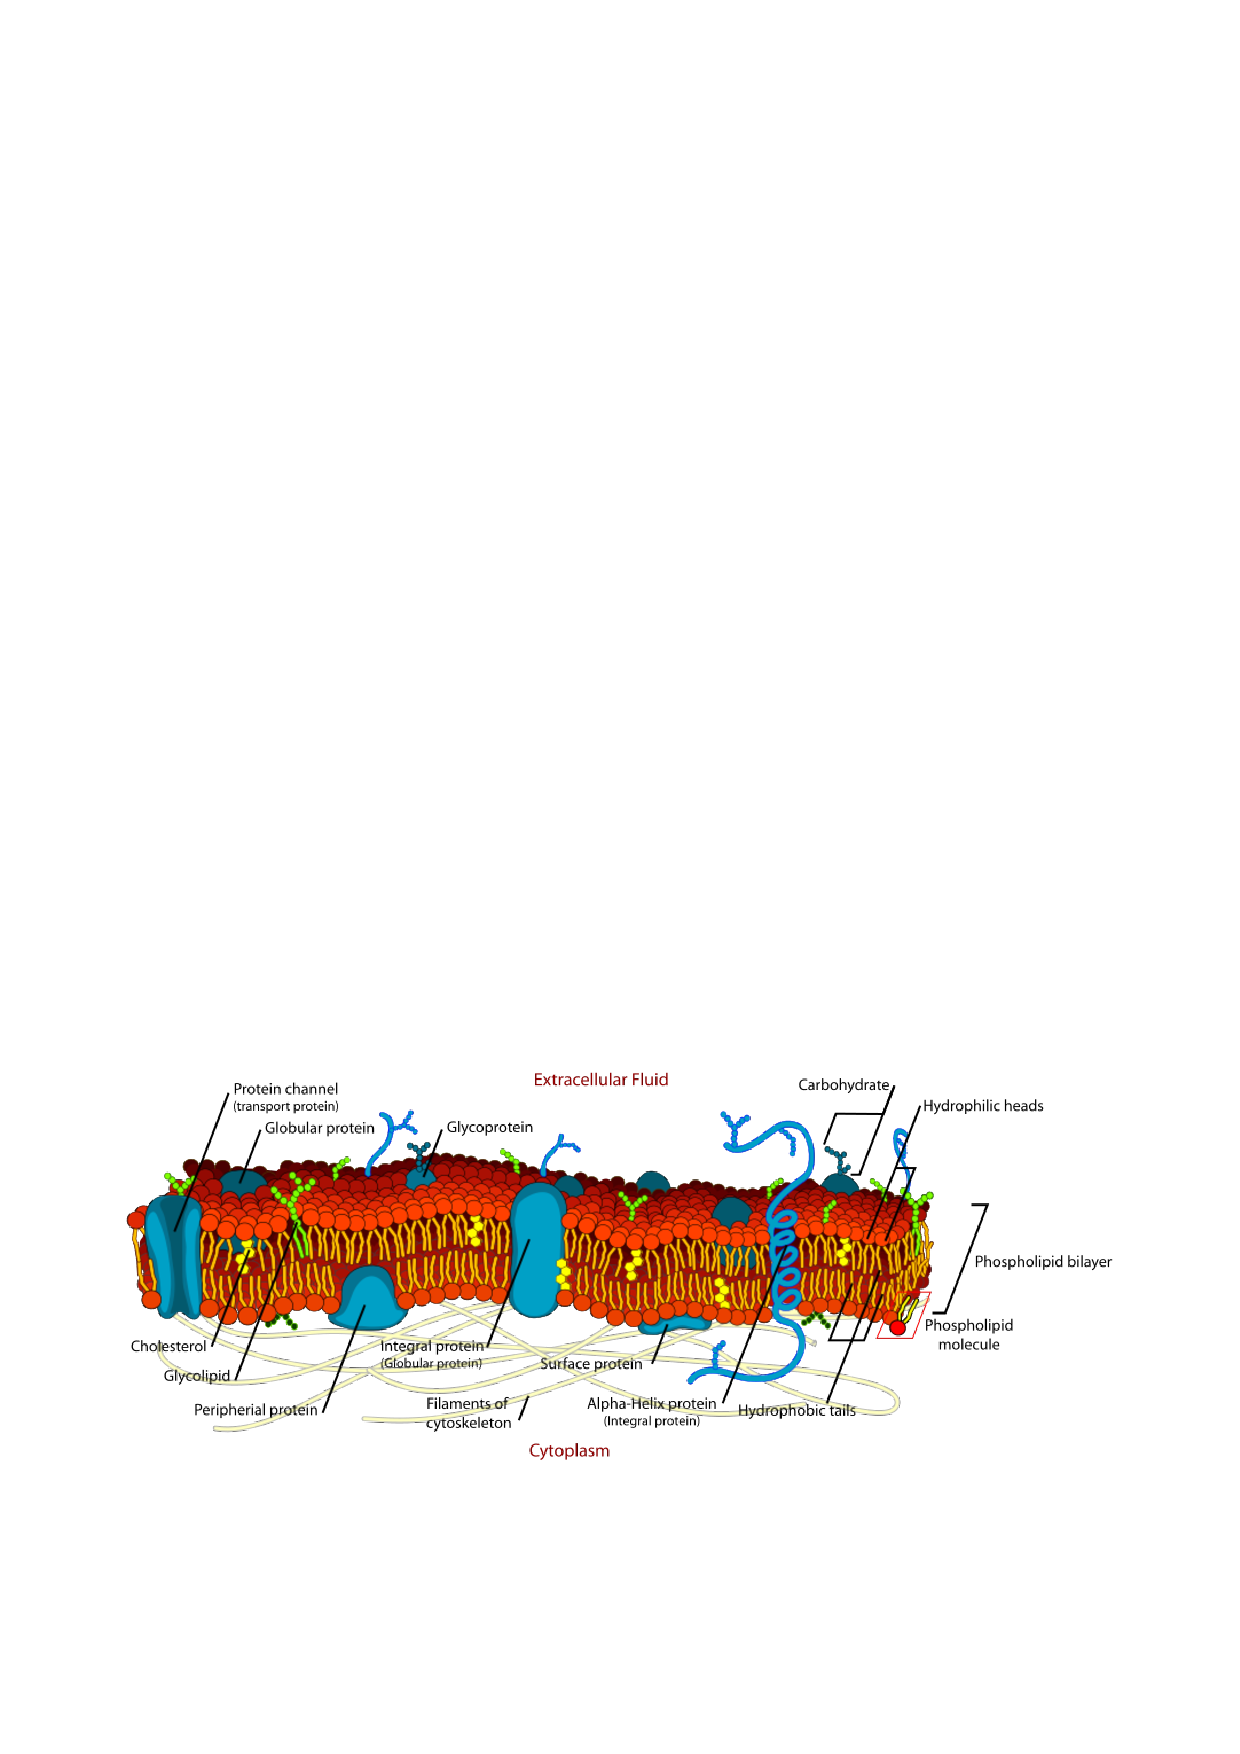
\includegraphics[width=4in]{\MemBio /Pics/Cell_membrane_detailed_diagram}
\caption{
شکل از سایت ویکیپیدیا گرفته شده است
\cite{wikiCellMembrane}. این یک نقاشی از غشا بر اساس مدل غشای مایع موزایکی است. بیشتر غشا از ملکول‌های چربی تشکیل شده ولی پروتئین‌های خیلی زیادی نیز در غشا قرار دارد.  غشا از طریق این پروتئین‌ها به اسکلت سلولی و اجزای دیگر متصل است. دایره‌های قرمز سر آب‌دوست و رشته‌های زرد دُم‌های آب‌گریز لیپید‌ها را نشان می‌دهد.
}
\label{fig:fluidmembranemodel}
\end{center}
\end{figure}


در نتیجه‌ی توسعه‌ی تحقیقات، می‌دانیم غشا‌های زیستی بیشتر ساختار موزائیکی دارند تا مایع. یعنی در سلول‌های مختلف غشا خیلی همگن نیست و در یک سلول قسمت‌هایی از غشا ممکن است  ترکیب پروتئینی متفاوتی از بخش‌های دیگر همان سلول داشته باشد. همچنین ضخامت برخی از بخش‌های غشا ممکن است از چند ۱۰ نانومتر تا ۱۰۰ نانومتر (که با سفینگولیپید\LTRfootnote{sphingolipids}
و کُلِسترول غنی است) تغییر کند
\cite{Engelman:2005aa}. یکی از دلایل غیر همگن بودن غشا نامتقارن شدن آن به علت حضور قسمت میانی آب‌گریز غشا در کنار پروتئین‌ها یا پلی‌پپتیدها\LTRfootnote{polypeptide}
است.  مرکز غشا از نواری از دم‌های آب‌گریز تشکیل شده. پروتئینی هم که درون غشا قرار گرفته قسمت آبگریز خود را درون غشا جا داده و قسمت آب‌دوستش را بیرون. کافی‌است که قسمت آب‌گریز پروتئین  کمی از ضخامت نوار آب‌گریز لیپید‌های  بیشتر یا کمتر باشد که ضخامت غشا را تغییر دهد
\cite{Mouritsen1984}. 
در این حالت یا پروتئین باید تغییر شکل دهد که خود را با ضخامت غشا تنظیم کند، یا هر دو (شکل 
\ref{fig:BilayerPlusProtein}) که در هر حالت باعث بروز برهمکنش‌‌های پروتئین-لیپید و لیپید-لیپید می‌شود
\cite{Huang1986,Aranda-Espinoza1996,Safran2000,Haselwandter2013,Haselwandter-Christoph2013}.
مدل موزائیکی مدل خوبی است که مشکلات حرکتی لیپید‌ها و پروتئین‌های چسبیده به غشا را توضیح می‌دهد
\cite{Simons2000,Simons1997}.


\begin{figure}[h]
\begin{center}
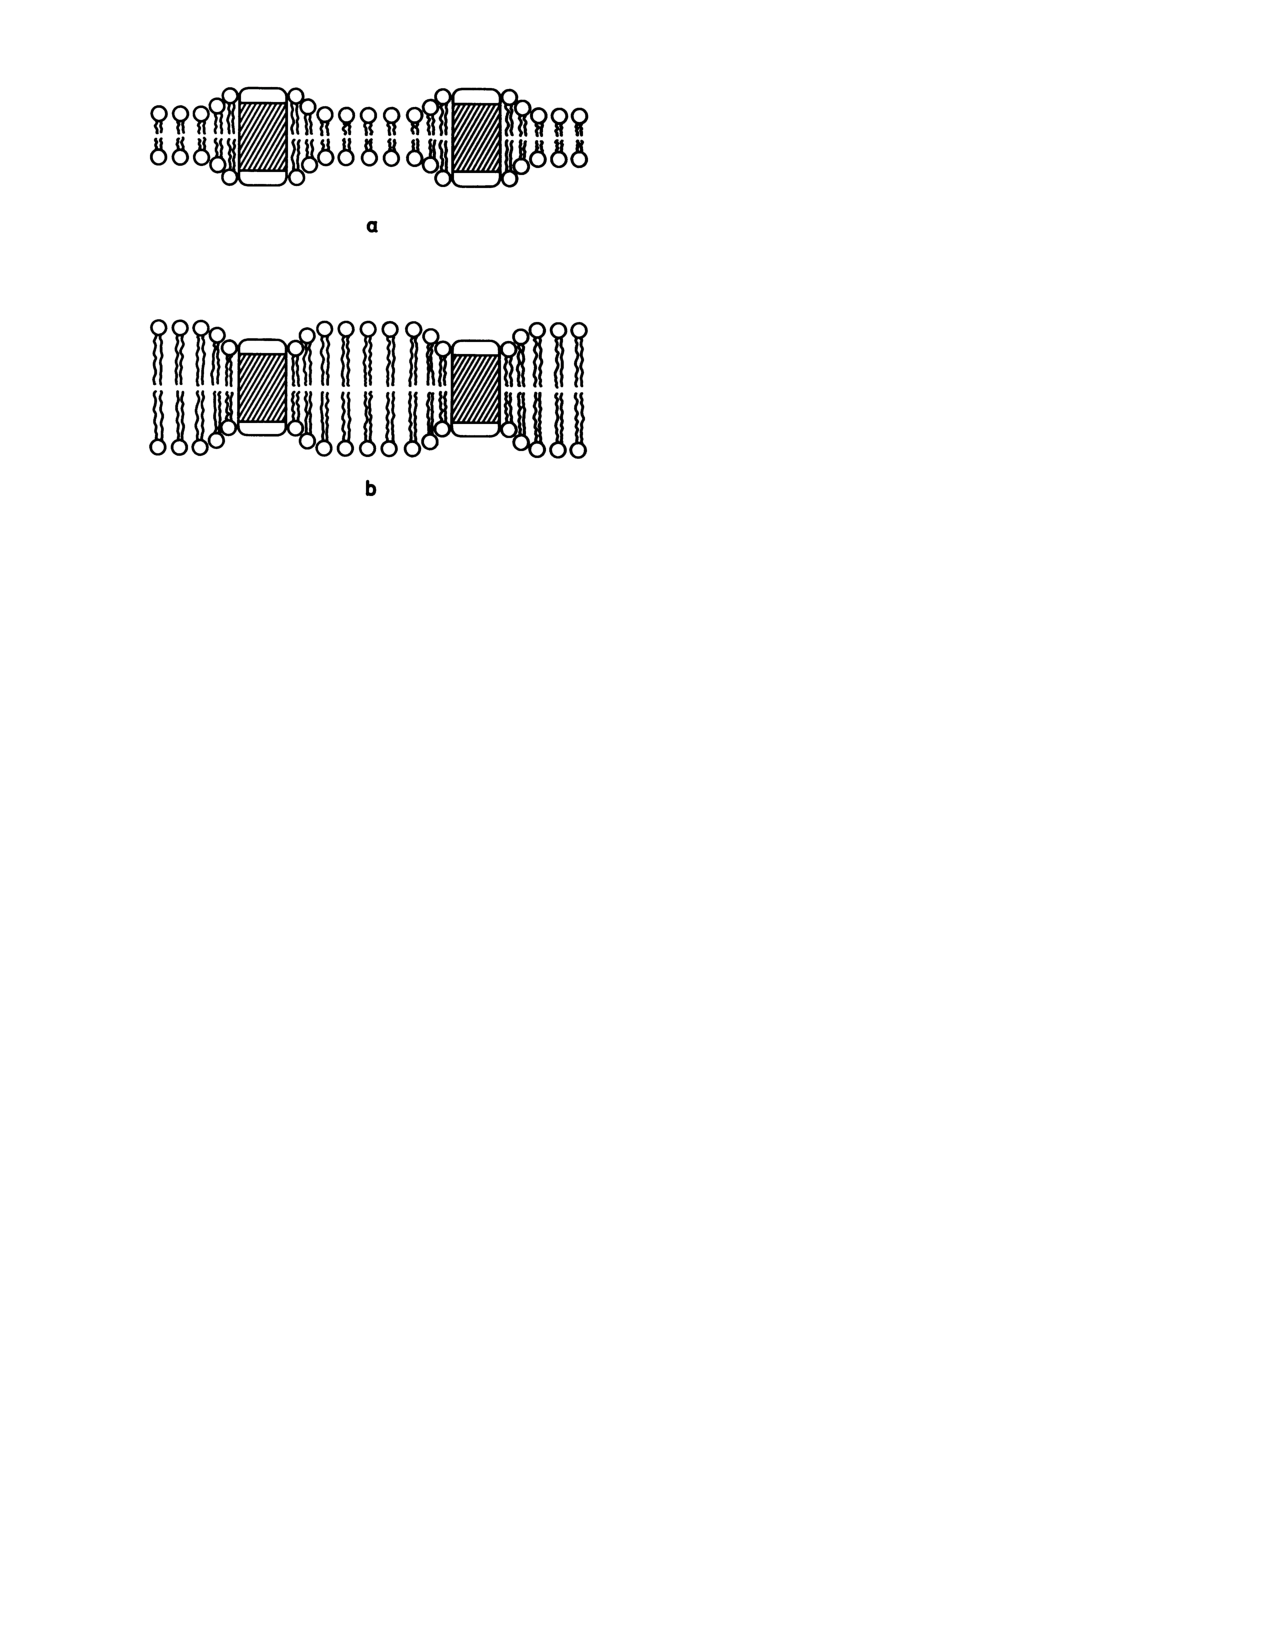
\includegraphics[width=4in]{\MemBio /Pics/BilayerPlusProtein}
\caption{
نقاشی از برش یک غشای لیپیدی که حاوی نوعی ناخالصی (مانند پروتئین یا پلی‌پپتید) است. ملکول‌های لیپید با دایره‌های سفید (سر آب‌دوست) و دم‌های آب‌گریز، و  ناخالصی‌ها به شکل مستطیل‌های دارای سر‌های آب‌دوست و ناحیه‌ی میانی هاشور خورده‌ی آب‌گریز نمایش داده شده‌است. اگر ناحیه‌ی آب‌گریز ناخالصی نسبت به غشا ضخیم‌تر (الف) یا نازک‌تر (ب) باشد، ضخامت غشا تحت تاثیر قرار می‌گیرد
\cite{Mouritsen1984}
.
}
\label{fig:BilayerPlusProtein}
\end{center}
\end{figure}





با وجود اینکه غشای لیپیدی به طور خود سامانده تشکیل می‌شود ولی علاوه بر ملکول‌های چربی پروتئین‌های زیادی نیز به غشا ساختار می‌بخشد
\cite{wikiCellMembrane}. غشاهایی هم می‌توان یافت که درصد پروتئین و کربوهیدارت در ساختار  آن به ترتیب بین ۱۸ تا ۷۵ درصد و  ۳ تا ۱۰ درصد باشد
\cite{MembraneProteins1972}. 
غشا از طریق این پروتئین‌ها به اجزای پیچیده‌تر داخل سلول (مانند اسکلت سلولی) متصل است. خاصیت تراوایی فوسفولیپید دو لایه و کانال‌های پروتئینی درون غشا، ارتباط سلول با محیط اطراف را کنترل و مدیریت می‌کند.  



\section{\label{sec:memBioSelfAssembily}
ساختارهای خودسامانده غشا
}
\setRL
%\pagenumbering{arabic} 
\section{
ساختارهای خودسامانده غشا
}
 
ملکول‌های لیپید یا چربی یکی از ۴ عناصری است که در کنار آمینو اسید‌ها، نوکلئیک اسید‌ها، و ملکول‌های قندی ساختار موجودات زنده را تشکیل می‌دهد که از این میان فقط لیپید‌ها پلیمر نیستند
\cite{Membraneasamatteroffat}. بیش از هزار نوع ملکول چربی در گونه‌های زیستی وجود دارد ولی ساختار کلی آنها بسیار مشابه است. در سلول‌ پستانداران بیشتر فسفولیپید و گلیسرول یافت می‌شود. ملکول‌ فوسفولیپید از یک سر آب‌دوست\LTRfootnote{hydrophilic}  
 و یک دُم آب‌گریز\LTRfootnote{hydrophobic}  
 ساخته شده‌است (شکل
\ref{fig:bilayer}). فرق بین ملکول‌های لیپید مختلف در ساختار شیمایی سر آب دوست و دُم آب‌گریز آنهاست. این ملکول‌ها در محلول‌های آبی
\textbf{بدون ایجاد پیوندها شیمیایی}، به طور خود سامانده\LTRfootnote{self-assembly}  
 تشکیل شده و ساختار‌های بسیار متنوعی دارند. اساس این ساختار‌ها کمینه کردن انرژی آزاد سیستم از طریق محافظت کردن دُم‌های آب‌گریز از آب است که با افزایش غلظت ملکول‌های لیپید ساختار‌های مختلفی تشکیل می‌شود
 (شکل
\ref{fig:bilayer}). برای مثال مایسِل‌ها\LTRfootnote{Micelle}
 در محلول‌های لیپدیدی با غلظت‌ پایین (ولی بالاتر از یک غلظت حدی) تشکیل می‌شود
 \cite{Lipowskyb1995ook}. در این ساختار انتهای تمام دُم‌های آب‌گریز در کنار هم قرار گرفته و سَر‌های آب‌دوست کُره تشکیل می‌دهند. هنگامی‌ که غلظت لیپید‌ها بیشتر شود یک تغییر حالت از مایسِل به ساختارهای دیگر مانند استوانه خواهیم دید. همچنین ساختار‌های ترکیبی نیز تشکیل می‌شود مانند در کنارهم قرار گرفتن استوانه‌ها در فاصله‌های
  $1-5nm$
طوری که محور استوانه‌ها بر روی شبکه‌ی شش ضلعی قرار می‌گیرد. 
 
 فرآوان‌ترین ساختار لیپید‌ها ساختار دو-لایه ‌است (شکل
 \ref{fig:bilayer}
 ب).  در ساختار‌های دو-لایه دُم‌های  آب‌گریز در مرکز لایه (به دور از آب) و سر آب‌دوست به سمت محلول جهت‌گیری می‌کند. از آنجایی که لبه‌های این سطوح شامل دُم‌های آب‌گریز است، به لحاظ انرژی هزینه‌بر است و به همین علت این سطوح هندسه‌های بسته تشکیل می‌دهند، مانند لیپوزم\LTRfootnote{Liposome}
 یا ساختار‌های ترکیبی مانند غشا‌هایی که از چندین دو-لایه تشکیل شده‌اند
\cite{LifeAsaMatterofFat2005}.

لازم به ذکر است که عوامل دیگری مانند دما و ترکیبات شیمیایی محلول بر نحوه‌ی تشکیل ساختار‌های لیپیدی تاثیر می‌گذارند. از آنجایی که دُم لیپید‌ها شکل ثابتی ندارد نمی‌توان حجم مشخصی برای این ملکول معین کرد. ولی تاثیر ترکیبات محلول، دما، و سایر عوامل موثر بر رفتار این ملکول را می‌توان با در نظر گرفتن حجم متوسط،
$v$، سهم سطح، 
$a$، و عمق اشغال شده ملکول درون ساختار،
$\ell$، مُدل کرد. این پارامتر‌ها با اندازه‌گیری روی اندازه‌ی سر دوقطبی، طول د‌ُم اسید چرب و حل‌شوندگی دُم در محلول تنظیم می‌شود
\cite{LifeAsaMatterofFat2005}. مثلا بالا رفتن دما  مُد‌های چرخشی زنجیر کربنی حول محور خود را افزاریش داده و در نتیجه سهم مساحت اشغالی ملکول بالا می‌رود
\cite{BiomembranesBook1989}. البته که این امر می‌تواند منجر به ذوب شدن غشا نیز شود
\cite{BioMemBook2007}.
 اسرائیلاچویلی\LTRfootnote{LiposomeIsraelachvili}
و همکارانش در یک مقاله‌ی معروف در سال ۱۹۷۶
\cite{Israelachvili1976}، با یک ضرب و تقسیم سر انگشتی تاثیر شکل ملکول‌های لیپیدی را توصیف می‌کنند. امکان قرار گرفتن یک ملکول لیپید در ساختاری مشخص با عدد بسته‌بندی یا پَکینگ\LTRfootnote{packing}
مشخص می‌شود:
\begin{equation}
%\begin\centering
P=\frac{v}{a\ell}
%\end\centering
\end{equation}
مثلا برای مایسِلی به شعاع، 
$R_m$، رابطه‌ی حجم، 
$v=\frac{1}{N}\frac{4\pi R_m^3}{3}$، و سطح 
$a=\frac{1}{N}4\pi R_m^2$ 
به این صورت تخمین زده می‌شود. در اینجا،
$N$، تعداد ملکول‌ها در ساختار مایسِل است. از آنجایی که شعاع مایسِل نمی‌تواند از طول دُم ملکول بزرگتر باشد (
$\ell\geq R_m$
):
\begin{equation}
%\begin\centering
P_m=\frac{v}{a\ell}=\frac{\frac{1}{N}\frac{4\pi R_m^3}{3}}{\frac{1}{N}4\pi R_m^2\ell}=\frac{1}{3}\frac{R_m}{\ell}\leq\frac{1}{3}
%\end\centering
\end{equation}
پس عدد پَکینگ باید کمتر از 
$\frac{1}{3}$
باشد تا ساختار‌‌های مایسِل پایدار داشته باشیم. این محاسبات برای  ساختارهای استوانه‌ای به شعاع، 
$R_c$
، و طول بلند، 
$L\gg R_c$
به این شکل انجام می‌شود،
\begin{equation}
%\begin\centering
P_c=\frac{v}{a\ell}=\frac{\frac{1}{N}\pi LR_c^2}{\frac{1}{N}2\pi LR_c\ell}=\frac{1}{2}\frac{R_c}{\ell}\leq\frac{1}{2}
%\end\centering
\end{equation}
در نتیجه ساختار استوانه‌ای پایدار در عدد پَکینگ 
$\frac{1}{3}<P<\frac{1}{2}$
ایجاد می‌شود. با تکرار محاسبات مشابه عدد عدد پَکینگ برای ساختار‌های دو لایه
$\frac{1}{2}<P<1$
تخمین زده می‌شود. لیپید‌هایی که از غشاهای زیستی استخراج می‌شود بیشتر 
$P>1$
دارند، در نتیجه‌ شکل کلی آن‌ها شبیه به یک مخروط وارونه است. در نتیجه دو-لایه‌هایی که فقط از ملکول‌های لیپید زیستی ساخته شده باشد تنش‌ها خمشی زیادی خواهد داشت
\cite{Mouritsen2011,Membraneasamatteroffat}. این تنش‌ها با اضافه شدن پروتئین‌ها و تشکیل حباب‌های کوچک (هم رو به داخل
\LTRfootnote{endocytosis}
  هم رو به بیرون
 \LTRfootnote{exocytosis}) بر روی غشای سلول آزاد می‌شود.



\begin{figure}[h]
\begin{center}
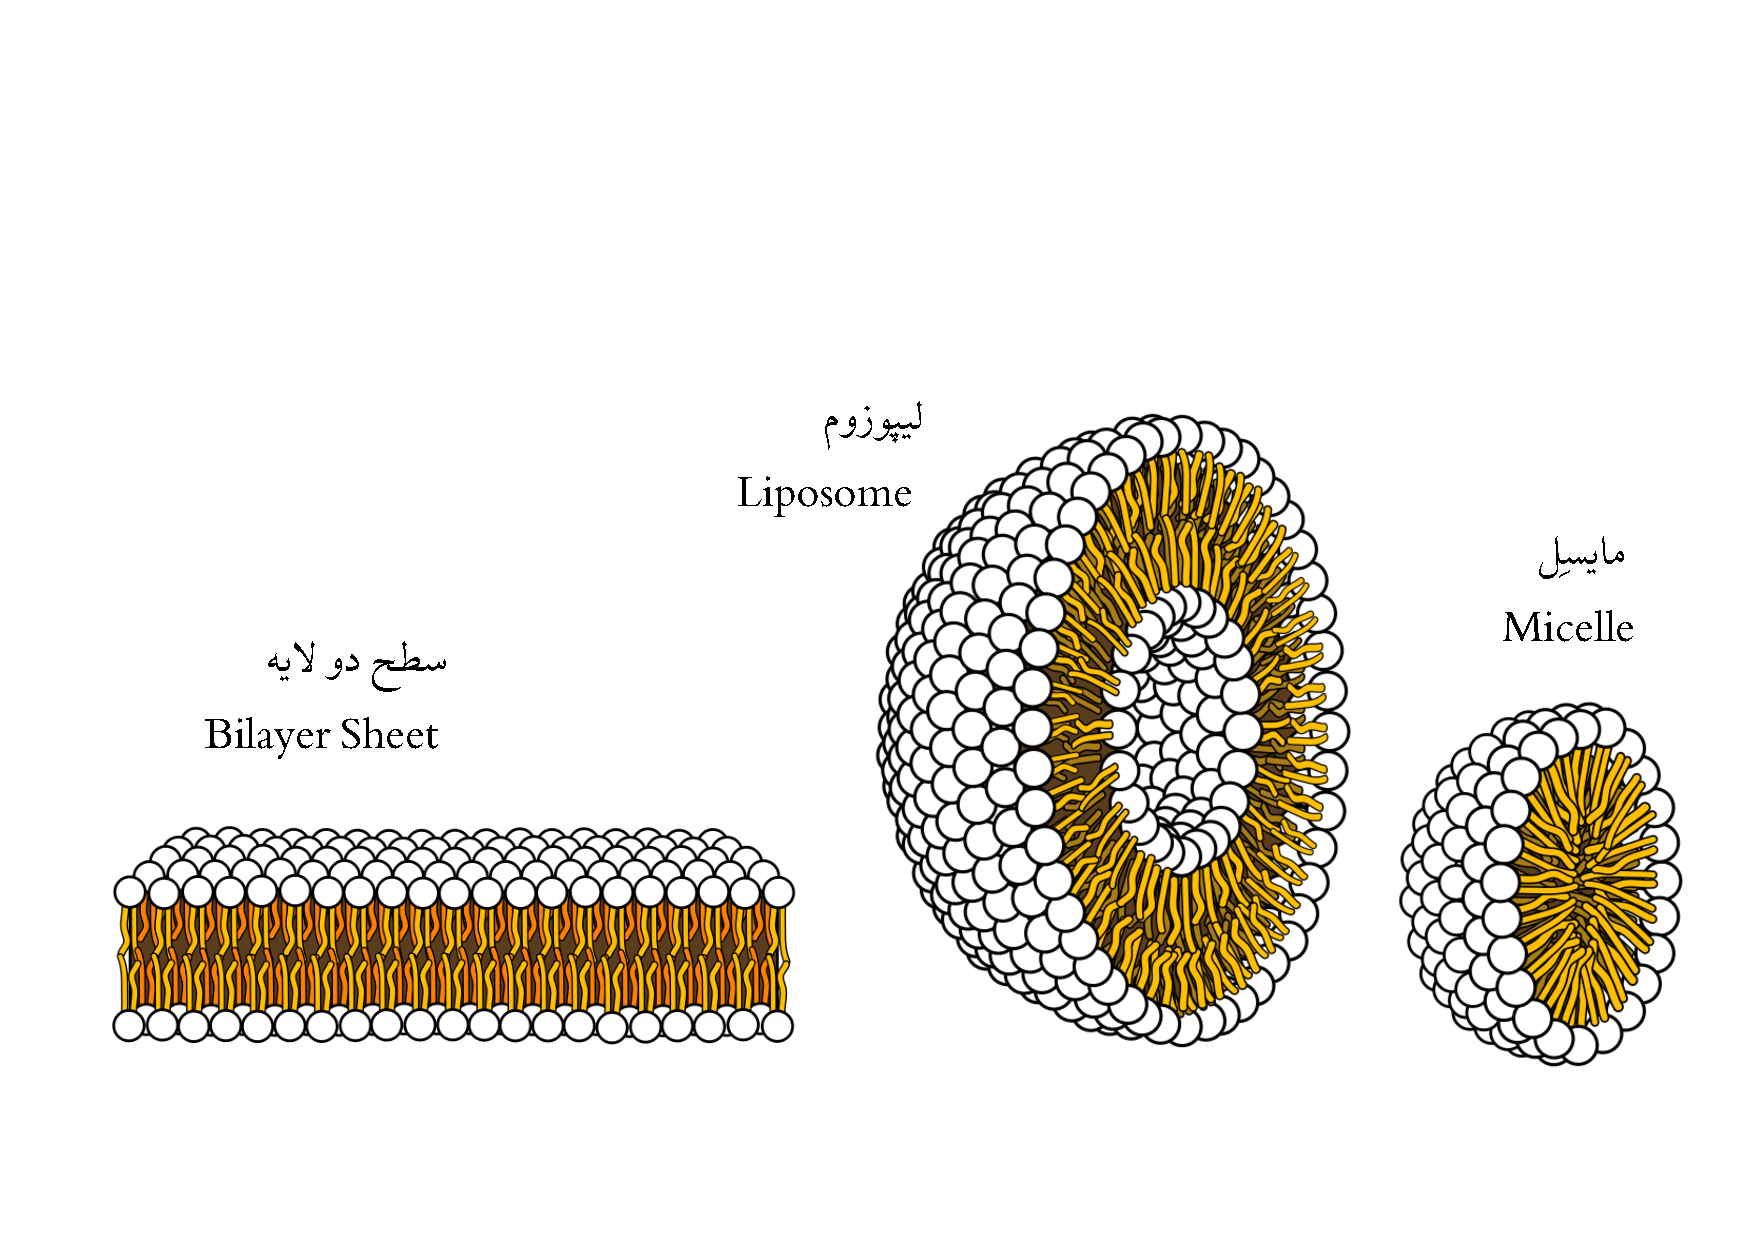
\includegraphics[width=4in]{\MemBio /Pics/Bilayer}
\caption{
الف) ساختار شیمیایی یک ملکول فوسفولیپید. سر آب‌دوست (دایره‌ی آبی) و  انتهای آب‌گریز مشخص شده است. ب) ساختار‌های معمول ملکول‌های چربی در آب. به ترتیب از چپ به راست، ساختار سطوح بزرگ دو-لایه، کُره‌های دو-لایه (لیپوزوم)، و کره‌های کوچک تک لایه، مایسِل.
}
\label{fig:bilayer}
\end{center}
\end{figure}




\begin{figure}[h]
\begin{center}
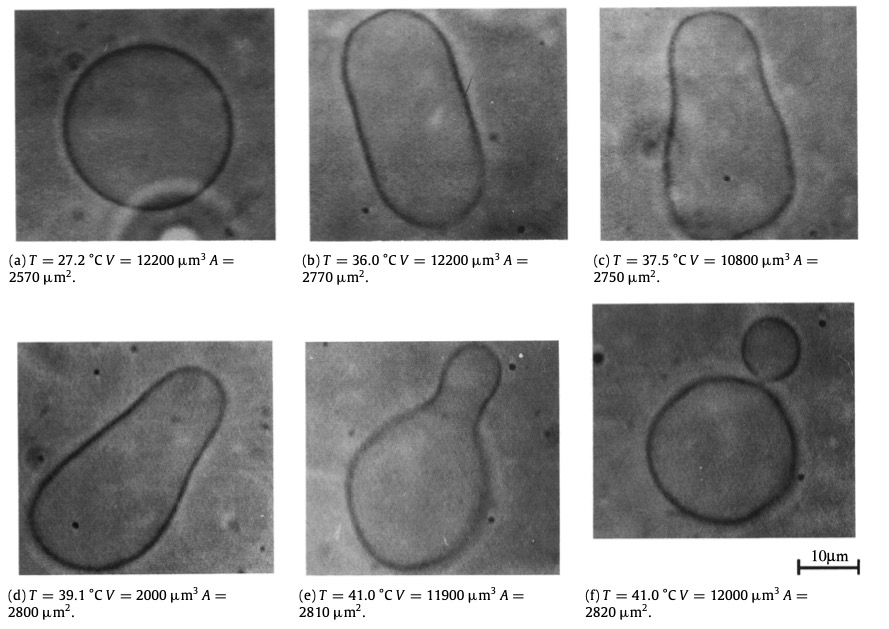
\includegraphics[width=4in]{\MemBio /Pics/GUVTempChange}
\caption{
تغییر ساختار یک غشای غول ‌آسا به علت تغییر دما از ۲۷/۲ تا ۴۱ درجه‌ی سانتیگراد. در دمای ۳۶ درجه حالت بیضی شکل، بالاتر از دمای ۳۶ شکل گلابی، و با ماندن در دمای ۴۱ درجه یک حباب بر روی آن جدا شده.
}
\label{fig:GUVTempChange}
\end{center}
\end{figure}






با وجود پیچیدگی‌ که در غشای سلول‌های زیستی هست، آن‌ها نیز باید از قوانین فیزیکی حاکم بر اجسام بی‌جان پیروی کنند. از طرفی غشا‌ها بیشتر دارای ساختارهای متنوع و خاص هستند تا ساختارهای مشترک که بتوان عمومیت داد
\cite{NelsonBook2004}.
ولی می‌توان خواص فیزیکی غشاها را با قوانین ترمودینامیک به صورت درشت دانه مدل کرد و رفتار‌ آن‌ها را در طیفی از هندسه‌ها و مقیاس‌ها مشخص کرد
\cite{Seifert1997}.
 مثلا انرژی مشخصه اندازه‌گیری شده برای تجمع واحد‌های تشکیل‌ دهنده‌ی غشاهای زیستی یک مرتبه‌ی بزرگی از انرژی گرمایی محیط 
$k_BT$
بیشتر گزارش شده. در اینجا، 
$k_B$،
ثابت بُلتسمَن و 
$T\approx300K$،
دمای محیط است. در نتیجه ساختار غشاهای زیستی در مقابل افت و خیز گرمایی در نزدیکی دماهای فیزیولوژیکی پایدار است. همچنین آنقدر نرم  هستند که توسط فرآیندهای زیستی مانند اتصال پروتئین‌ها
\cite{NelsonBook2004,Seifert1997,Deserno2015}،
ATP
هیدرولسیز
\LTRfootnote{ATP hydrolysis}
\cite{Boyle2008Biology,Lipowskyb1995ook}
تغییر شکل می‌دهند.
یکی از خواص مهم و جالب غشاها مقاومت خیلی کمِ خم شدنِ آن‌ها تحت نیروی خارجی است. این پدیده، افت و خیز دیواره‌ی سلولی، با میکروسکوپ نوری به راحتی قابل مشاهده است
\cite{NelsonBook2004}.
جذابیت دیگر غشا‌ها برای فیزیکدان‌ها ضخامت خیلی کم آن‌هاست که در نتیجه می‌توان آن را با یک صفحه‌ی ۲ بعدی مدل‌سازی کرد و ابعاد مسئله‌ را کاهش داد
\cite{Seifert1997,Deserno2015}.
درنتیجه‌ی مطالعه‌ی غشاها با استفاده از این نوع ساده‌سازی و مدل سازی می‌توانیم  رفتار آن‌ها را در مقیاس‌های مختلف پیش‌بینی کرده و نقش‌ آن‌ها را در فرآیند‌های زیستی توصیف کنیم.



محققان با مطالعه‌ی غشا‌های غول‌آسا
\LTRfootnote{Giant Unilamellar vesicle}  
 یا 
 GUV اطلاعات  زیادی راجع به ساماندهی غشاهای چربی جمع‌آوری کرده‌اند. این غشا‌ها را معمولا می‌توان با  مخلوط کردن\LTRfootnote{mixing}  
 غشا‌ و ترکیب‌های چربی در آزمایشگاه ساخت
 \cite{GUVmaking2009}
و اندازه‌ی آن می‌تواند از چند میلی‌متر تا چند میکرون  باشد. 
GUV نسبت به تغییرات ترمودینامیکی محیط واکنش‌های بسیار جالبی نشان می‌دهد. برای مثال شکل
\ref{fig:GUVTempChange}
ایجاد یک حباب کوچک بر روی یک GUV را با تغییر دمای محیط از ۲۷ تا ۴۱ درجه در قالب ۶ سری عکس پشت سر هم نشان می‌دهد
\cite{MemReviewRamakrishnan2014}.
 
\begin{figure}[h]
\begin{center}
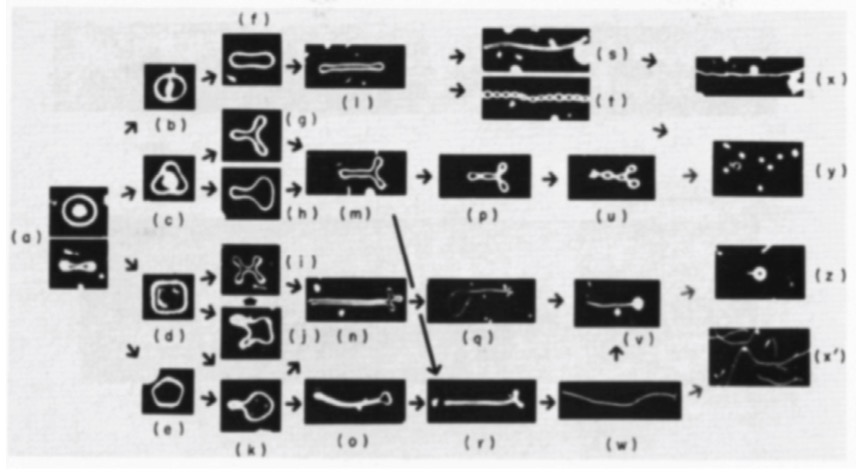
\includegraphics[width=4in]{\MemBio /Pics/GUVPresChange}
\caption{
مسیر‌های مختلفی که یک غشای غول آسای آب نباتی شکل (ستون سمت چپ، زاویه‌ی دوربین از بالا و کنار) که بر اثر تغییر غلظت نمک محیط طی می‌کند تا به شکل خیلی کشیده (ستون سمت راست) در بیاید، را نشان می‌دهد.
}
\label{fig:GUVPresChange}
\end{center}
\end{figure}

GUV همچنین نسبت به تغییرات فشار اسمزی محیط نیز واکنش نشان می‌دهد. مثلا در شکل 
\ref{fig:GUVPresChange}
می‌بینیم که با تغییر غلظت نمک در محیط یک غشایِ لیپیدیِ دارای کلسترول، از شکل اولیه آب نباتیِ\LTRfootnote{biconcave}  
شبیه‌ به گلبول قرمز به حالت کشیده و لوله‌ای در می‌آید. در شکل 
\ref{fig:GUVPresChange}
ساختار‌های هندسی میاینی (و در مواردی ناپایدار) مختلفی که غشا طی می‌کند تا از هندسه‌های سمت چپ به هندسه‌های سمت راست برسد، را می‌توان مشاهده کرد.
  
 
 
 
 
 
 
 
 
 
 

\section{\label{sec:memBioGUVs}
غشاهای غول‌آسا
}
%\setRL
%\pagenumbering{arabic} 

\begin{figure}[t]
\begin{center}
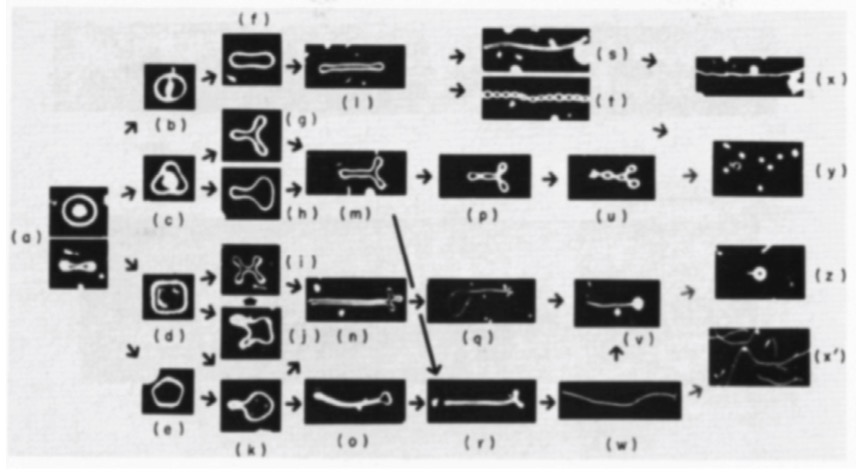
\includegraphics[width=\columnwidth]{\MemBio /Pics/GUVPresChange}
\caption{
مسیر‌های مختلفی که یک غشای غول آسای آب نباتی شکل (ستون سمت چپ، زاویه‌ی دوربین از بالا و کنار) که بر اثر تغییر غلظت نمک محیط طی می‌کند تا به شکل خیلی کشیده (ستون سمت راست) در بیاید.
}
\label{fig:GUVPresChange}
\end{center}
\end{figure}

\begin{figure}[t]
\begin{center}
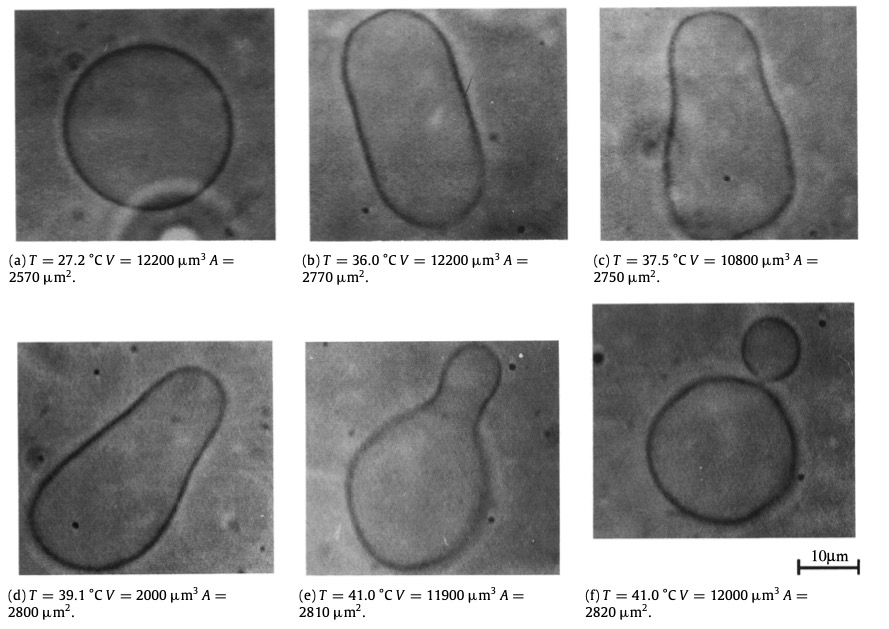
\includegraphics[width=\columnwidth]{\MemBio /Pics/GUVTempChange}
\caption{
تغییر ساختار یک غشای غول ‌آسا به علت تغییر دما از ۲۷/۲ تا ۴۱ درجه‌ی سانتیگراد. در دمای ۳۶ درجه حالت بیضی شکل، بالاتر از دمای ۳۶ شکل گلابی، و با ماندن در دمای ۴۱ درجه یک حباب بر روی آن جدا شده‌است.
}
\label{fig:GUVTempChange}
\end{center}
\end{figure}


محققان با مطالعه‌ی غشا‌های غول‌آسا
\LTRfootnote{Giant Unilamellar vesicle}  
 یا 
 GUV اطلاعات  زیادی راجع به ساماندهی غشاهای چربی جمع‌آوری کرده‌اند. این غشا‌ها را معمولا می‌توان با  مخلوط کردن\LTRfootnote{mixing}  
 غشا‌ و ترکیب‌های چربی در آزمایشگاه ساخت
 \cite{GUVmaking2009}
و اندازه‌ی آن می‌تواند از چند میکرون تا چند میلی‌متر   باشد.
این غشاها از یک دولایه‌ی خیلی ساده لیپیدی تشکیل شده‌اند و در نتیجه‌ ضخامت‌ آن‌ها بین ۴ -۵ میلی‌متر است (دو برابر اندازه‌ی یک مولکول لیپید). غشاهای زیستی ساختار پیچیده‌تری دارند ولی در اصل تمام‌ غشاهای زیستی بر بستر یک ساختار دو لایه‌ی لیپیدی بنا شده‌اند و در نتیجه می‌توان خواص مشترک زیادی میان غشا‌های غول‌آسا و غشاهای زیستی پیدا کرد.
غشاهای دولایه، مرز مشخصی میان شاره‌‌‌ای که درون خود بسته‌بندی کرده‌اند و شاره‌ای که در محیط اطراف است تشکیل می‌دهند. ساختار غشا نسبت به مولکول‌های کوچک غیر باردار مانند 
$H_2O$، 
$O_2$،
و 
$CO_2$
و همچنین
$H_3O^+$
و
$OH^-$
تراوا است ولی نسبت به مولکول‌های درشت‌ترِ حلال در آب مانند گلوکز\LTRfootnote{glucose}
و منوساکارید‌ها\LTRfootnote{monosaccharid}
 تراوا نیست. در نتیجه‌ حضور چنین مولکول‌هایی در محیط، فشار اسمزی بر غشا وارد خواهد کرد. فشار اسمزی به اختلاف غلظت مولکول‌های درون و خارج از غشا بستگی دارد و باعث جابجایی آب داخل غشا می‌شود. در صورتی که غلظت حل شونده در خارج از غشا بیشتر باشد، شبیه به یک پمپ، آب از درون غشا خارج می‌شود و نسبت حجم به سطح غشا را تغییر می‌دهد. برعکس، در صورتی که غلظت مولکول‌ها درون غشا بیشتر از محیط باشد، آب از محیط به درون غشا پمپ می‌شود. تغییر شکل غشا در این صورت تا جایی ادامه پیدا می‌کند که شکل یک کُره به خود بگیرد. اگر همچنان آب به داخل غشا منتقل شود کمی سطح غشا کشیده می‌شود (کُره رشد می‌کند) تا جایی که تحمل کشش غشا تمام شود و غشا پاره خواهد شد.





همانطور که در شکل 
\ref{fig:GUVPresChange}
نشان داده‌ شده‌است، با تغییر غلظت نمک در محیط یک غشایِ لیپیدیِ دارای کلسترول، از شکل اولیه آب نباتیِ\LTRfootnote{biconcave}  
شبیه‌ به گلبول قرمز به حالت کشیده و لوله‌ای در می‌آید. در شکل 
\ref{fig:GUVPresChange}
ساختار‌های هندسی میاینی (و در مواردی ناپایدار) مختلفی که غشا طی می‌کند تا از هندسه‌های سمت چپ به هندسه‌های سمت راست برسد، را می‌توان مشاهده کرد.
GUV نسبت به تغییرات ترمودینامیکی محیط واکنش‌های بسیار جالبی نشان می‌دهد. برای مثال شکل
\ref{fig:GUVTempChange}
ایجاد یک حباب کوچک بر روی یک GUV را با تغییر دمای محیط از ۲۷ تا ۴۱ درجه در قالب ۶ سری عکس پشت سر هم نشان می‌دهد
\cite{MemReviewRamakrishnan2014}.



 

 
 
 
 
 
 
 
 
 
 
 
 

\section{\label{sec:memBioFluidity}
خواص سیال‌گون غشا
}
\setRL
%\pagenumbering{arabic} 
\section{
خواص سیال‌گون غشا
}

دیگر خاصیت مشترک میان تمام غشا‌ها این است که به علت سرعت بالای پخش ملکول‌ها بر روی سطح آن، حالت سیال بودن خود را حفظ می‌کند. سیال بودن غشا تقریبا از ده‌ی ۱۹۷۰ به بعد توسط عموم پذیرفته شد. در آن زمان آزمایش‌هایی به طور همزمان و مستقل شواهدی ارائه دادند که خاصیت سیال‌گون غشا را نشان می‌داد. اولین مشاهده در این تحقیقات مربوط به اندازه‌گیری سرعت پخش ملکول‌های لیپیدی  با برچسب اسپینی
\LTRfootnote{spin-labelled lipids}
\cite{Kornberg1971DiffusionPhospholipids, Devaux1972LateralDiffusion}
و ملکول‌های استروید
\LTRfootnote{steroids}  
\cite{Sackmann1972, Traeubl1972}
بر سطح غشا بود که حدود 
$1 \mu m^2\cdot sec^{-1}$
اندازه‌گیری شد. روش‌های جدید اندازه‌گیری  حرکت ملکول‌های فلورسانت
\LTRfootnote{fluorescence recovery after photobleaching (FRAP)}  
\cite{almeida1992lateral }
و همچنین روش‌های شناسایی تک ذره‌ای 
\LTRfootnote{single particle tracking}  
\cite{Sako1994, Saxton1997, Fujiwara2002, Kusumi2005}
این ضریب پخش را در مورد غشاها تایید می‌کنند.

دومین سر آزمایش‌هایی که ماهیت سیال‌گون غشا را تایید کرد  مطالعات بر روی نحوه‌ی تغییر شکل گلبول‌های قرمز 
\cite{Canham1970, Evans1974}
و غشاهای لیپیدی
\cite{Helfrich1973, Helfrich1976}
انجام شده ماهیت سیال‌گونه‌ی غشا را نیز تایید می‌کند. در اثر تغییر شکل، خمش سطح غشا  به طور پیوسته و بدون شکستگی تغییر می‌کند و در صورتی که جنس غشا جامد و یا پلیمری باشد چنین تغییر شکلی امکان پذیر نخواهد بود. به طور مشخص این نوع تغییر شکل زمانی مشاهده می‌شود که حباب‌های جانبی بر روی سطح غشا تشکیل می‌شود (شکل 
\ref{fig:budding}
).

\begin{figure}[h]
\begin{center}
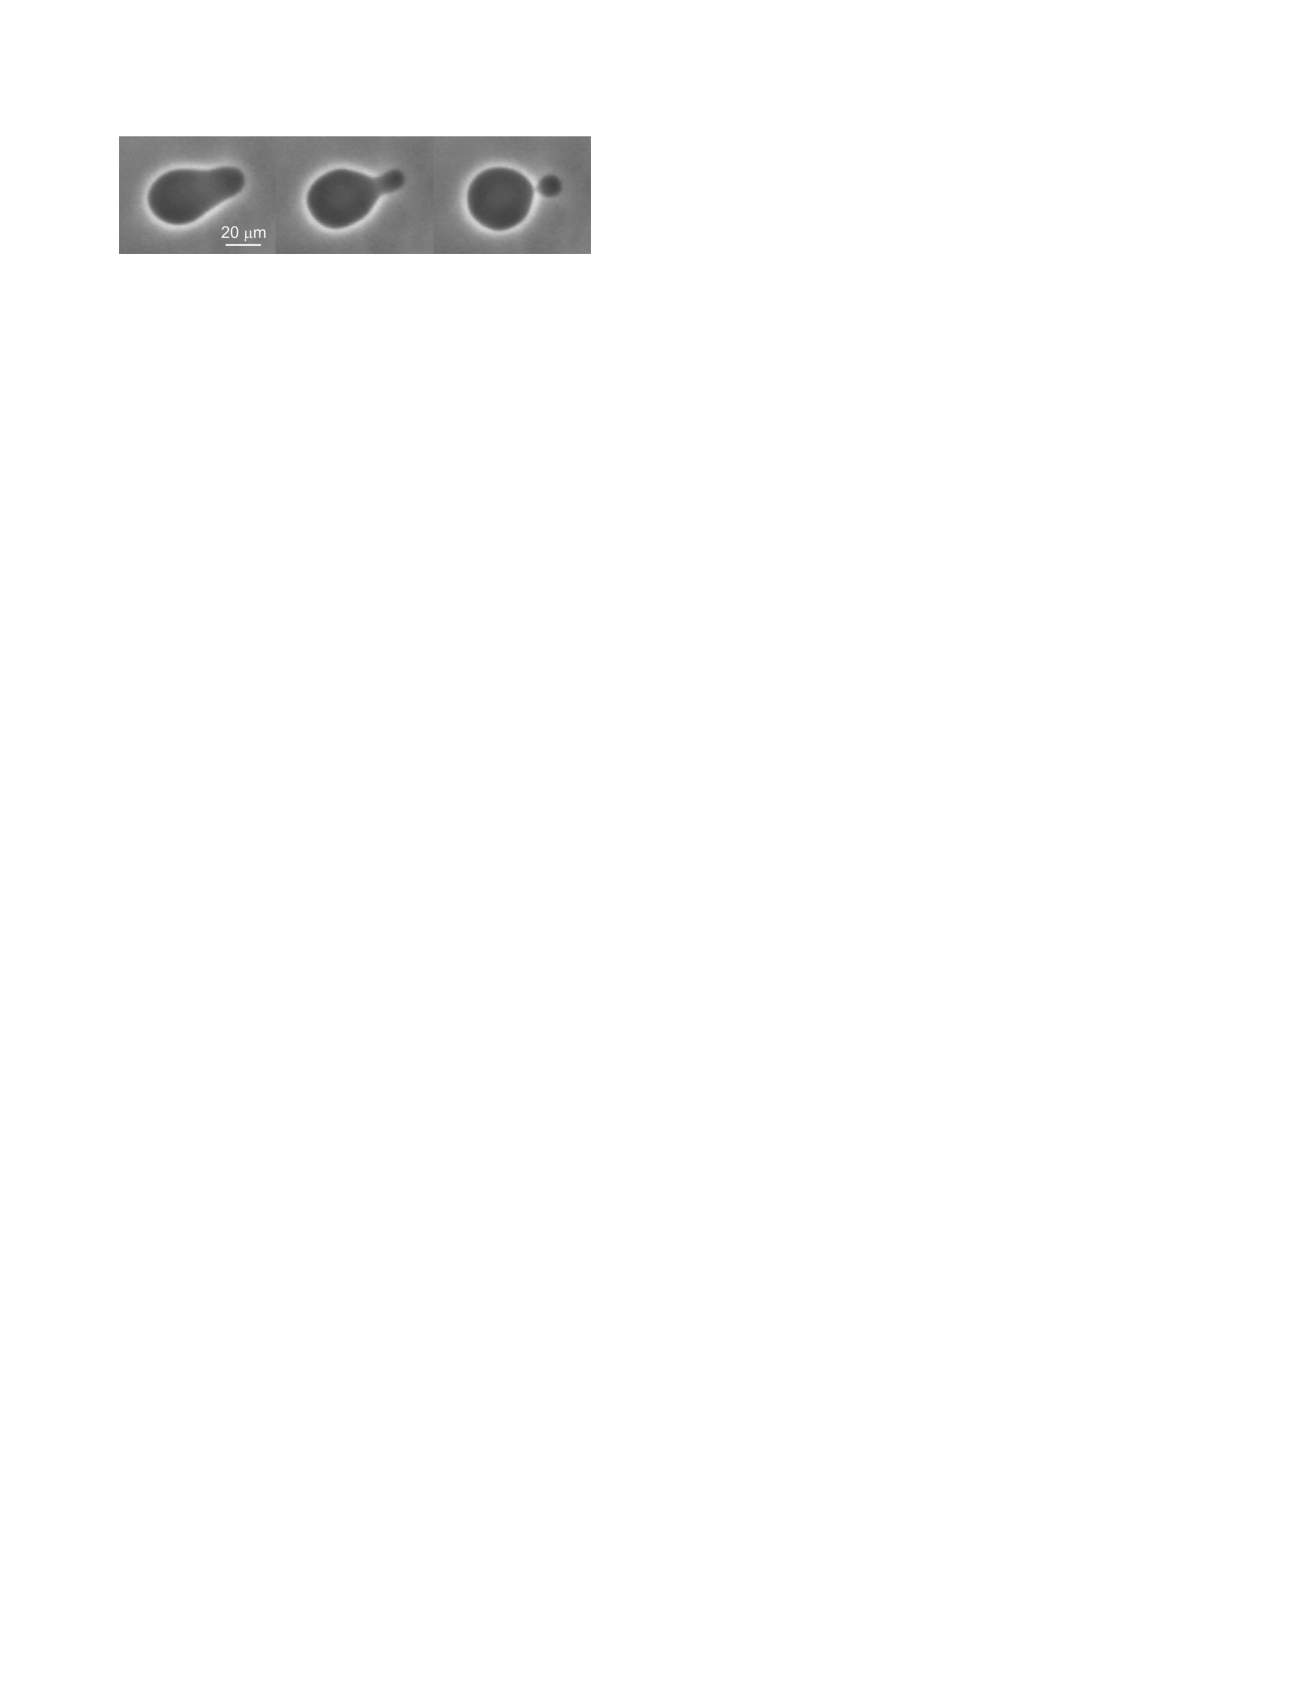
\includegraphics[width=6in]{\MemBio /Pics/budding.pdf}
\caption{
تشکیل یک غشای حبابی بر سطح یک غشای غول‌آسا در تصویربرداری میکروسکوپی اختلاف فازی. این حباب ظرف ۵ ثانیه تشکیل  شده که نشان از جنس سیال‌گون غشا است.
\cite{Dimova2006} 
}
\label{fig:budding}
\end{center}
\end{figure}

این نوع جوانه‌زدن
\LTRfootnote{budding}  
یکی از مهم‌ترین ساز‌ و کار‌های مبادله‌ی ملکول با محیط در سلول‌های زیستی‌ است. در یک سری از فرآیند‌های زیستی سلول پروتئین‌ها رو به سطح داخلی غشا منتقل می‌کند و با ایجاد جوانه می‌تواند ملکول‌های خود را به محیط صادر کند. عکس این فرآیند هم انجام می‌شود که بر اثر آن سلول اطلاعاتی از سلول‌های حاضر در محیط اطراف خود دریافت می‌کند.








\section{\label{sec:nuclearenvelope}
بسته‌ی هسته‌ی سلول
}
%\setRL
%\pagenumbering{arabic} 


\begin{figure}[t]
\begin{center}
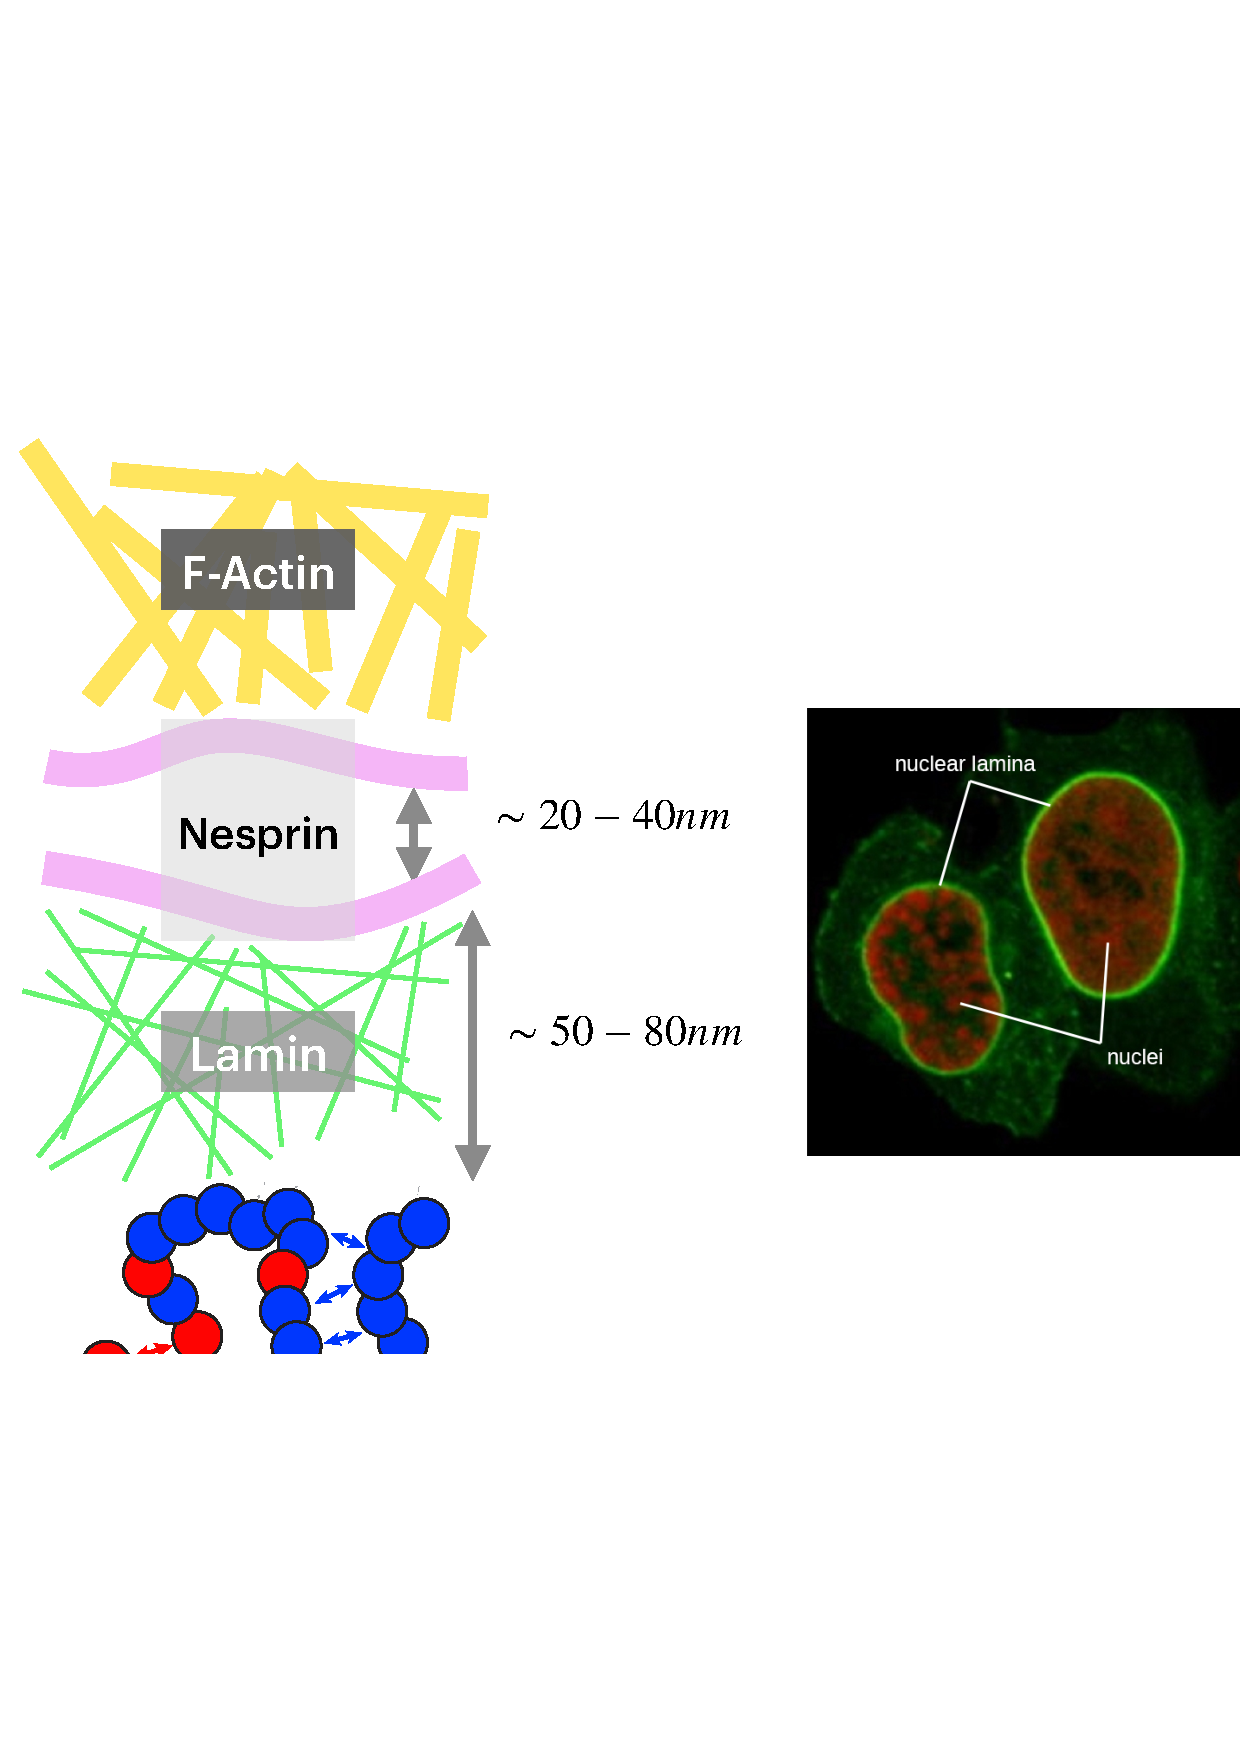
\includegraphics[width=6in]{\MemBio /Pics/NuclearEnvelope}
\caption{
عکس سمت راست، تصویر رنگ آمیزی شده‌ی هسته. لایه‌ی لمینا با رنگ سبز روشن، و کروماتین‌های درون هسته با رنگ قرمز نمایش داده‌ شده‌است. شکل سمت چپ، نقاشی ساختار بسته‌ی هسته است. از بالا به پایین: شبکه‌ی اکتین (زرد) که با پروتئین‌های نسپرین به غشای دولایه‌ی بیرونی (نوار صورتی) متصل شده‌است. غشای داخلی نیز به کمک همین پروتئین به لایه‌ی لمینا (سبز) متصل شده‌است. فضای میان غشای داخلی و خارجی از ۲۰ تا ۴۰ نانومتر تغییر می‌کند. ضخامت لمینا نیز بین ۵۰ تا ۸۰ نانومتر است. کروماتین‌های درون هسته (دایره‌های آبی و قرمز) می‌توانند با لایه‌ی لمینا اتصالاتی برقرار می‌کند. 
}
\label{fig:nuclearenvelope}
\end{center}
\end{figure}


غشای هسته یا نام رایج آن، بسته‌ی هسته\LTRfootnote{nuclear envelope}
ساختاری متفاوت نسبت به غشای سلول دارد. در خارج و اطراف هسته، ساختارهای زیادی وجود دارد، مانند شبکه‌ی اکتین\LTRfootnote{actin network}
 و میکروتیوبول‌ها\LTRfootnote{microtubules}.
 هسته‌ی سلول از طریق بسته‌ی هسته با تمامی‌ ارگان‌های لازم در ارتباط است.

در شکل 
\ref{fig:nuclearenvelope}
نقاشی از ساختار کلی بسته‌ی هسته را می‌بینیم. از بالا به پایین، خطوط زرد رنگ نماینده‌ی شبکه‌ی پروتئینی اکتین است. این شبکه از طریق پروتئین‌هایی به نام نسپرین\LTRfootnote{nesprin},
 که روی بسته‌ی هسته وجود دارند، به بسته‌ی هسته متصل است و نقش پُلی برای انتقال نیرو‌های خارج از سلول به هسته‌ی سلول را ایفا می‌کند
\cite{Lammerding2011}. 
بسته‌ی هسته از دو عدد غشای لیپیدی دو لایه (نوارهای صورتی) با نام غشای بیرونی و غشای داخلی تشکیل شده. ضخامت فضای بین دو غشا از ۲۰ تا ۴۰ نانومتر تغییر می‌کند. میان دو غشا را مایعی شبیه به سیتوپلاسم و شبکه‌ پروتئینی مورد نیاز برای انتقال مواد بین هسته و سلول، پر می‌کند. پروتئین‌های نسپرین  در غشای داخلی هم حضور دارد و این غشا را به شبکه‌ی پروتئینی لمینا\LTRfootnote{lamina}
(شکل
\ref{fig:nuclearenvelope}
نقاشی سمت چپ، خطوط سبز‌ رنگ) متصل می‌کند. لمینا‌ شبکه‌ای است به ضخامت حدود ۵۰ تا ۸۰ نانومتر که تمام سطح غشای داخلی را پوشانده است. در تصویر سمت راست شکل 
\ref{fig:nuclearenvelope}
با استفاده از روش‌های رنگ آمیزی میکروسکوپی، لایه‌ی لمینا را به رنگ سبز روشن می‌بینیم که کروماتین‌های (قرمز) درون هسته را محصور کرده‌اند. لمینا خاصیت الاستیکی دارد و تقریبا تمام ویژگی الاستیک بسته‌ی هسته به علت وجود این بخش است
\cite{Steensel2017wd}.
مدول الاستیک شبکه‌ی اکتین تقریبا ۵۰۰ پاسکال، و مدول الاستیک هسته‌ی سلول زمانی که درون سلول قرار دارد، ۵ هزار پاسکال و هنگامی ‌که از سلول خارج شده باشد، ۸ هزار پاسکال اندازه‌گیری شده‌است
\cite{Dahl2004, CAILLE2002177}.









\clearpage
\clearpage
\chapter{
\centering{
غشا از نگاه نظری
}
}
\setRL
\clearpage

\def \MemTB {\Mempath /MembraneTheoreticalBackground}

%\section{
%چکیده
%}
%در این فصل مدل‌های پیوسته‌ی نظری استفاده شده برای توصیف غشاها را بررسی می‌کنیم.

\subsection{
تنش حاصل از تغییر مساحت
}
در حالت تعادلی، مولکول‌های لیپیدی، با توجه به شرایط ترمودینامیکی محیط، سطح غشا را با چیدمانی بهینه‌ می‌پوشانند.  به علت وجود نیروهای خارجی یا قیود مختلف،  سطح غشا از سطح تعادلی
$A_0$
تغییر کرده، و در سطح غشا تنش  
$\gamma_{st}(A)$
ایجاد خواهد شد. از آنجایی که غشا ماهیت سیال‌گون دارد،  تنشی که حاصل آن تنها جابجایی مولکول‌ها روی سطح باشد (تنش برشی\LTRfootnote{shear})
 انرژی سطح را تغییر نخواهد داد. تنها تنشی که مساحت کل غشا را تغییر دهد با مقاومت روبرو خواهد شد. تنش غشا تا مرتبه‌ی اول در جمله‌ی 
$(A-A_0)$
به شکل زیر تعریف می‌شود،
\begin{equation}
\gamma_{st}(A)=k_A\frac{A-A_0}{A_0}.
\end{equation}
در این معادله
$k_A$
مدول فشردگی سطحی\LTRfootnote{area compressibility modulus}
است
\cite{thegiantvesiclebook2019}.
 بدیهی‌است که این رابطه تا زمانی که تنش ایجاد شده از  آستانه‌ی پاره شدن غشا کمتر باشد قابل استفاده است. برای غشاهای لیپیدی، آستانه‌ی پاره شدن دو مرتبه‌ی بزرگی کوچک‌تر از مدول فشردگی سطحی و حدود چند
$mN/m$
است. انرژی تنش ایجاد شده حاصل از تغییر مساحت غشا، معادل کار انجام شده برای تغییر سطح است،
\begin{equation}
E_{st}(A)=\int_{A_0}^A dA~\gamma_{st}(A)=\frac{1}{2}k_A\frac{(A-A_0)^2}{A_0}.
\label{eq:surfaceTension}
\end{equation}
مشابه به این بحث می‌توان هزینه‌ی انرژی برای تغییر حجم سیال درون غشا را نیز به صورت زیر تعریف کرد
\cite{discher1998biophysicaljournal},
\begin{equation}
E_{v}(V)=\frac{1}{2}k_V\frac{(V-V_0)^2}{V_0}.
\label{eq:volumeEnergy}
\end{equation}
  در اینجا
$k_V$
مدول فشردگی حجمی\LTRfootnote{volume compressibility modulus}
 و 
$V_0$
حجم تعادلی سیال درون غشا است.








\subsection{
تنش حاصل از تغییر مساحت و حجم
}
در حالت تعادلی، مولکول‌های لیپیدی، با توجه به شرایط ترمودینامیکی محیط، سطح غشا را با چیدمانی بهینه‌ می‌پوشانند.  به علت وجود نیروهای خارجی یا قیود مختلف،  سطح غشا از سطح تعادلی
$A_0$
تغییر کرده، و در سطح غشا تنش  
$\gamma_{st}(A)$
ایجاد خواهد شد. از آنجایی که غشا ماهیت سیال‌گون دارد،  تنشی که حاصل آن تنها جابجایی مولکول‌ها روی سطح باشد (تنش برشی\LTRfootnote{shear})
 انرژی سطح را تغییر نخواهد داد. تنها تنشی که مساحت کل غشا را تغییر دهد با مقاومت روبرو خواهد شد. تنش غشا تا مرتبه‌ی اول در جمله‌ی 
$(A-A_0)$
به شکل زیر تعریف می‌شود،
\begin{equation}
\gamma_{st}(A)=k_A\frac{A-A_0}{A_0}.
\end{equation}
در این معادله
$k_A$
مدول فشردگی سطحی\LTRfootnote{area compressibility modulus}
است
\cite{thegiantvesiclebook2019}.
 بدیهی‌است که این رابطه تا زمانی که تنش ایجاد شده از  آستانه‌ی پاره شدن غشا کمتر باشد قابل استفاده است. برای غشاهای لیپیدی، آستانه‌ی پاره شدن دو مرتبه‌ی بزرگی کوچک‌تر از مدول فشردگی سطحی و حدود چند
$mN/m$
است. انرژی تنش ایجاد شده حاصل از تغییر مساحت غشا، معادل کار انجام شده برای تغییر سطح است،
\begin{equation}
E_{st}(A)=\int_{A_0}^A dA~\gamma_{st}(A)=\frac{1}{2}k_A\frac{(A-A_0)^2}{A_0}.
\label{eq:surfaceTension}
\end{equation}
مشابه به این بحث می‌توان هزینه‌ی انرژی برای تغییر حجم سیال درون غشا را نیز به صورت زیر تعریف کرد
\cite{discher1998biophysicaljournal},
\begin{equation}
E_{v}(V)=\frac{1}{2}k_V\frac{(V-V_0)^2}{V_0}.
\label{eq:volumeEnergy}
\end{equation}
  در اینجا
$k_V$
مدول فشردگی حجمی\LTRfootnote{volume compressibility modulus}
 و 
$V_0$
حجم تعادلی سیال درون غشا است.








\subsection{
تغییر شکل غشا
}
\begin{figure}[h]
\begin{center}
\includegraphics[width=4.5in]{\MemTB /Pics/polymorphism}
\caption{
تغییر شکل یک غشا حاصل تغییر دمای محیط. شکل غشا ابتدا دمبلی است 
$(D)$
سپس دو شکل میانی ستومتوسایت
$S_1$
و
$S_2$
تشکیل شده و در نهایت پس از اتصال دو بازو، دو کُره‌ی تو در تو 
$L^{sto}$
تشکیل می‌دهد 
\cite{Berndl1990EPL}.
}
\label{fig:shapeChanges}
\end{center}
\end{figure}

درسته که غشاها رفتار سیال‌گون دارند ولی رفتار آنها با یک قطره‌ی مایع متفاوت است. در غیاب نیروی خارجی و قیود، قطره‌ی مایع به منظور کاهش انرژی سطح مشترک آن با محیط به شکل کُره در می‌آید. برخلاف یک قطره، غشا می‌توانند اشکال مختلفی همچون دیسکوسایت
\LTRfootnote{discocyte}
، ستومَتوسایت
\LTRfootnote{stomatocyte}
، و  دَمبِلی داشته باشد. همچنین شرایط ترمودینامیکی محیط (فشار اسمزی و دما) می‌تواند باعث تغییر شکل آن شود. از آنجایی که ملکلول‌های لیپیدی حل‌شوندگی ناچیزی دارند می‌توان فرض کرد که تعداد ملکلول‌های لیپیدی هنگام تغییر شکل غشا ثابت است. علاوه بر آن فاصله‌ی تعادلی ملکلول‌های لیپیدی تابع دمای محیط است. از طرفی تغییر مساحت غشا بر اثر نیرو‌های خارجی یا قیود مختلف بیسار ناچیز است و تغییر مساحت زیاد باعث پاره شدن غشا می‌شود. در نتیجه هنگام تغییر فشار اسمزی (کاهش یا افزایش سیال داخل آن)  در دمای ثابت، مساحت غشا با تقریب بسیار خوبی ثابت است. به طور عمومی حجم غشا می‌تواند به مقدار خیلی زیادی کاهش یابد ولی هرگز نمی‌تواند از حجم یک کُره بیشتر شود. 

در صورتی که دمای محیط تغییر کند، هم مساحت غشا هم حجم سیال درون آن تغییر خواهد کرد. نسبت سطح به حجم حاصل از دمای جدید شکل تعادلی غشا را مشخص خواهد کرد. در صورتی که دمای محیط به میزان 
$\Delta T$
تغییر کند، سطح و حجم غشا از حالت تعادلی
$A_0$
و
$V_0$
به مقدار 
$\Delta A=\alpha_A\Delta T A_0$
و حجم سیال درون آن 
$\Delta V=\alpha_V\Delta T V_0$
تغییر می‌کند. برای یک غشای لیپیدی که سیال درون آن آب باشد،
$\alpha_A\approx2\times 10^{-3}/K$
و
$\alpha_V\approx2\times 10^{-4}/K$
. یک محاسبه‌ی سر انگشتی نشان می‌دهد که در صورت افزایش دمای محیط نسبت حجم به سطح غشا کاهش پیدا می‌کند. نمونه‌ای از تغییر شکل غشا حاصل از افزایش دمای محیط در شکل 
\ref{fig:shapeChanges}
نمایش داده شده‌است.


\subsection{
حجم کاهیده
}
همانطور که در فصل اول توضیح داده شد. غشاهای زیستی نمیه‌تراوا هستند. یعنی حجم آب درون آنها توسط دمای محیط، غلظت ملکول‌های محیط، و ملکول‌های درون آن یا به طور عمومی شرایط اسمزی محیط مشخص می‌شود. در صورتی که اختلاف فشار اسمزی از بیرون بالا باشد، غشا ممکن است مچاله شود، بر روی خود تا شود، و یا غشا‌های کچک‌تری تشکیل دهد. ملکول‌های لیپید بسته به شرایط محیطی (مثلا دما) با چیدمان مشخصی فضا را اشغال می‌کنند. با فرض اینکه تعداد ملکول‌های غشا تغییر نکند، سطح غشا در طول عمر آن ثابت خواهد بود. از طرفی تحت اختلاف فشار اسمزی منفی، غشا متورم خواهد شد. البته میزان تغییر سطح غشا فقط در حدود چند درصد است و در صورتی که نیاز به تغییر سطح بیشتری باشد، پاره خواهد شد. برای غشایی با مساحت
$A$
شعاع کُره‌ای معادل که همان مساحت را داشته باشد،
\begin{equation}
R_{ve}=\sqrt{\frac{A}{4\pi}}
\end{equation}
است. از آنجایی که بیشترین حجمی که غشا می‌تواند داشته باشد حجم یک کُره‌ است، حجم غشا همیشه کمتر مساوی این مقدار خواهد بود،
\begin{equation}
V\leq\frac{4\pi}{3}R_{ve}^3=\frac{4\pi}{3}\left(\frac{A}{4\pi}\right)^{\frac{3}{2}}
\end{equation}
در نتیجه می‌توان حجم کاهیده به شکل زیر تعریف کرد،
\begin{equation}
\nu=\frac{V}{\frac{4\pi}{3}R_{ve}^3}=6\sqrt{\pi}VA^{-\frac{3}{2}}
\label{eq:reducedVolume}
\end{equation}
که همیشه کوچک‌تر از یک است و در صورتی که غشا شکل کُره‌ای بی نقص داشته باشد برابر یک خواهد بود.



\section{
انحنای غشا
}
\subsection{
تعریف خمش
}

ضخامت غشا از مرتبه‌ی چند نانومتر است و مقیاس انحنا‌هایی که شکل کلی غشا را مشخص می‌کنند از مرتبه‌ی بزرگی میکرون بوده. در نتیجه به طور عمومی مدل کردن شکل و انحنای غشا با یک رویه‌ی ۲ بعدی کاملا قابل قبول است. تصاویر میکروسکوپی غشا مانند شکل‌های 
\ref{fig:budding}
و
\ref{fig:flucmem} 
نشان می‌دهد که غشا سطحی نسبتا صاف و پیوسته دارد. در نتیجه در مقیاس‌های میکرومتری غشا را با رویه‌ای با چنین ویژگی‌ای مدل می‌کنیم. البته که این فرض در مقیاس نانومتری پابرجا نیست. 

\begin{figure}[t]
\begin{center}
\includegraphics[width=\columnwidth]{\Mempath/Pics/Membrane_fluctuations}
\caption{
مجموعه تصاویر پست سر هم از تغییر شکل یک غشای لیپیدی را با تصویر برداری فلورسانت در بازه‌های ۵ ثانیه‌ای نشان می‌دهد. خط مقیاس سفید رنگ اندازه‌ی ۵ میکرومتر را نشان می‌دهد. 
\cite{ParthasarathyMembraneMeasurement}
}
\label{fig:flucmem}
\end{center}
\end{figure}

مولکول‌های غشا درون یک سیال غوطه‌ور است. مولکول‌ها تحت افت خیز ترمودینامیکی محیط، در جهت‌ درون-صفحه‌ای سطح غشا و جهت عمود بر آن در حال حرکت است. در نتیجه برای تعریف انحنا، لازم است  سطح غشا به بخش‌های کوچک تقسیم بندی شود و با میانگین‌گیری بر روی  مکان مولکول‌ها انحنا را تعیین کرد. اندازه‌ی این بخش‌ها تابع شدت افت و خیز مولکول‌هاست. محاسبات حاصل از  شبیه‌ سازی دینامیک ملکلولی برای غشایی که مولکول‌های یکسان دارد حدود
$5.1$ 
 برابر ضخامت غشا گزارش شده است
\cite{Goetz1998}.
 انحنای هر بخش از یک غشای ساده با ضخامت 
$4nm$,
 حاصل از رفتار دست جمعی حدود 
$100$
مولکول لیپیدی خواهد بود. در مقیاس بزرگ، هر کدام از این بخش‌ها تنها یک نقطه بر روی رویه‌ی غشا را تشکیل می‌دهند. ما می‌توانیم برای هر نقطه روی غشا یک صغحه‌ی مماس و یک صفحه‌ی عمود بر مماس تعریف کنیم. صفحه‌ی عمود بر سطح با رویه‌ی غشا فصل مشترکی به شکل یک خط دارد (مانند شکل 
\ref{fig:normalPlaneIntersection}).
\begin{figure}[h]
\begin{center}
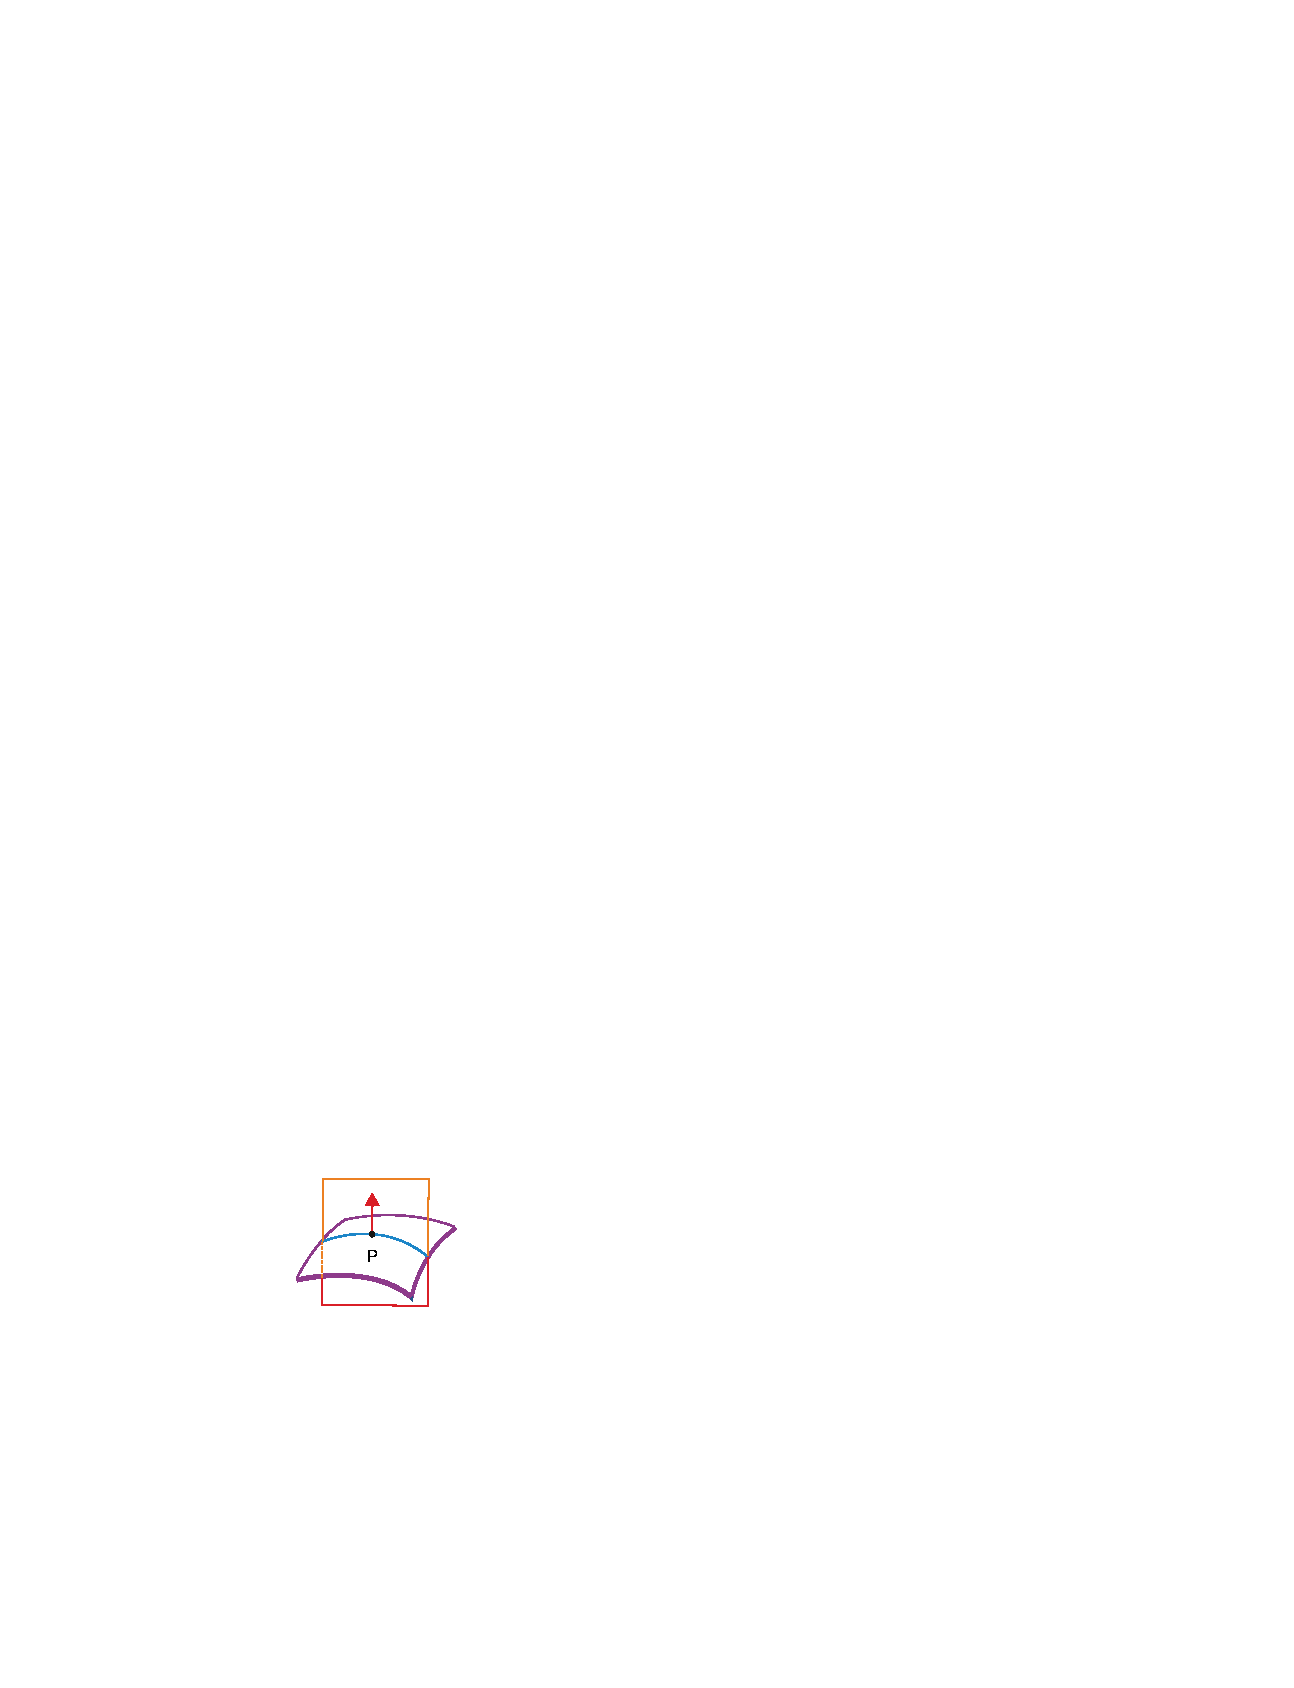
\includegraphics[width=6in]{\MemTB/Pics/NormalPlane}
\caption{
خم حاصل از فصل مشترک صفحه‌ی عمود بر سطح غشا در نقطه‌ی 
P
را نشان می‌دهد.
}
\label{fig:normalPlaneIntersection}
\end{center}
\end{figure}
انحنای تشکیل شده زد فصل مشترک، 
$C$
 در صورتی که در جهت بردار عمود بر سطح باشد 
($\cap$)
 با علامت مثبت و در حالتی که در جهت مخالف باشد 
($\cup$)
 با علامت منفی تعریف می‌شود. می‌توان فرض کرد که خط مشترک قسمتی از یک دایره  است و انحنای این خط عکس شعاع آن دایره خواهد بود. تنها یک  صفحه‌ مماس بر سطح  می‌توان تعریف کرد ولی صفحه‌ی عمود بر سطح می‌تواند در جهت‌های مختلف تعریف شود. انتخاب جهت صفحه‌ی عمود مقدار انحنای محاسبه شده را تغییر خواهد داد. اگر تمام انحناهای ممکن در یک نقطه‌ را با تغییر جهت صفحه‌ی متعامد اندازه‌گیری کنیم، مقادیر در بازه‌ای محدود به  کمینه و بیشینه‌ی انحنا قرار خواهد گرفت،
$C_{min}$
و
$C_{max}$.
 مقادیر کمینه و بیشینه انحنا به انحناهای اصلی سطح معرف هستند که با 
$C_1$
و
$C_2$
نمایش داده می‌شوند. انحناهای اصلی همچنین  ویژه‌مقدار‌های تانسور انحنا در آن نقطه هستند. همچنین اگر انحناهای اصلی برابر یکدیگر نباشند،
$C_1\neq C_2$ 
صفحاتی که خم‌ها با آن تعریف می‌شوند حتما عمود بر هم خواهند بود. از آنجایی که مولکول‌های سطح غشا حرکت پخشی می‌کنند  شکل غشا باید بر اساس تعاریفی باشد که تحت تغییر روش پارامتریزه\LTRfootnote{paprameterisation}  
 کردن سطح ناوردا باشد. انحناهای اصلی سطح چنین ویژگی دارند. انحنای میانگین در هر نقطه‌ بر روی سطح به صورت 
\begin{equation}
M=\frac{1}{2}(C_1+C_2)
\label{eq:meanCurv}
\end{equation}
و انحنای گاووسی به صورت
\begin{equation}
G=C_1C_2
\label{eq:gaussianCurv}
\end{equation}
 تعریف کرد. انحنای میانگین، معادل رَد\LTRfootnote{trace} 
 تانسور انحنا و انحنای گاووسی برابر با دترمینان این تانسور است. همچنین می‌توان روابط بالا را بازنویسی کرد و انحناهای اصلی را بر حسب انحنای میانگین و انحنای گاووسی محاسبه کرد،

\begin{figure}[t]
\begin{center}
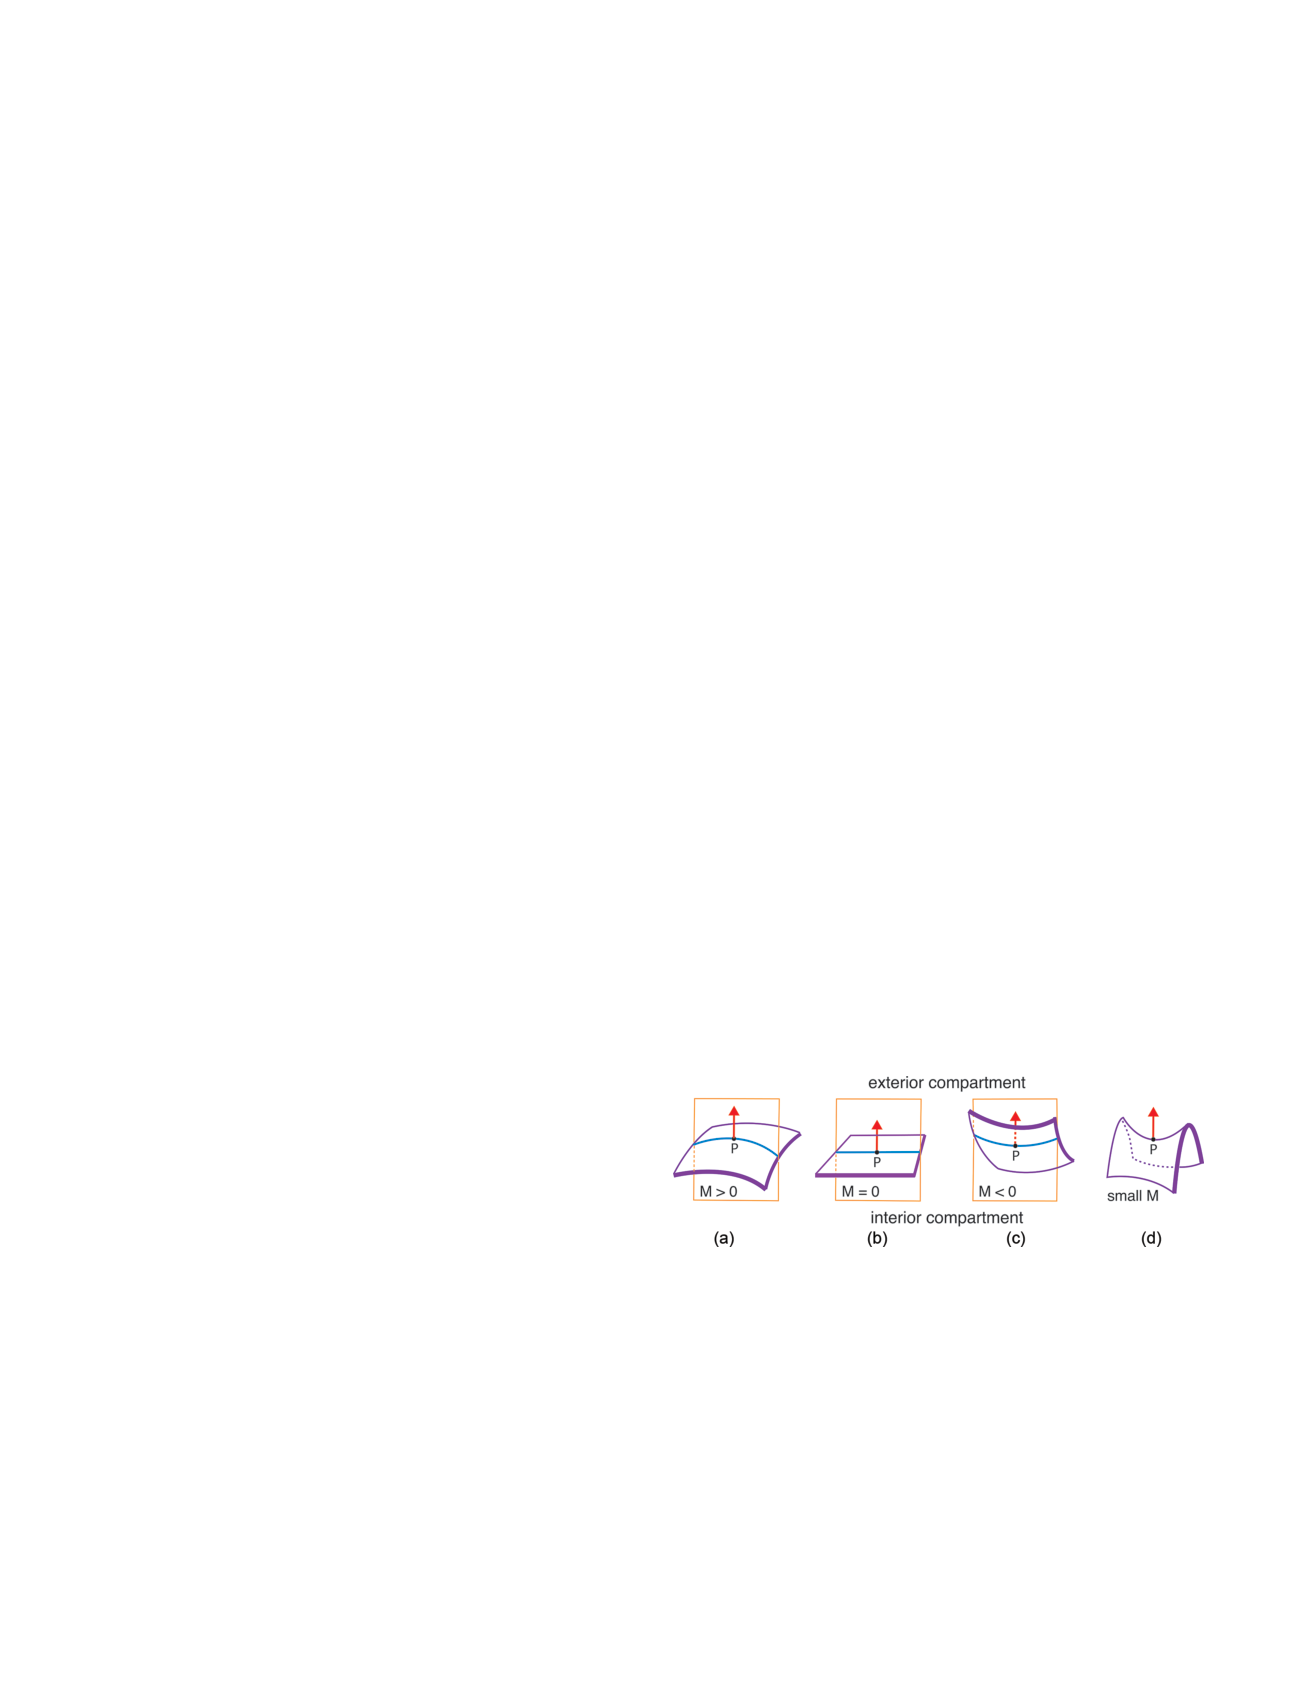
\includegraphics[width=\columnwidth]{\MemTB/Pics/curvatureSign}
\caption{
قرارداد برای تعیین علامت انحنای میانگین. با فرض اینکه بالا محیط خارج غشا و پایین داخل غشا را مشخص کند، بردار نرمال غشا جهت (بردار قرمز رنگ) رو به بالا خواهد داشت. در شکل الف) انحنای میانگین مثبت هنگامی که هر دو انحنای اصلی برآمدگی در جهت بردار نرمال داشته باشند. ب) برای قسمت تخت انحنای میانگین صفر، ج) انحنای منفی هنگامی که  برآمدگی به سمت داخل غشا باشد، د) در نقاط زین اسبی انحناهای اصلی علامت‌های مخالف یکدیگر دارند و در این صورت انحنای میانگین مقدار کمی خواهد داشت.
}
\label{fig:curvatureSign}
\end{center}
\end{figure}

\begin{equation}
\begin{aligned}
C_1&=M-\sqrt{M^2-G}\\
C_2&=M+\sqrt{M^2-G}.
\label{eq:gaussianCurv}
\end{aligned}
\end{equation}
که در روابط بالا، از آنجایی که 
$M^2\geq G$
\cite{Seifert1991}
 هر دو مقدار همیشه حقیقی هستند. مقدار انحنای میانگین، 
 $M$،
 تحت تمامی تبدیل‌های دستگاه مختصات که دترمینان ژاکوبین آن مثبت باشد (جهت بردار عمود بر سطح را تغییر ندهد) تغییر نخواهد کرد. به طور مثال اگر یک سطح با پارامتر‌های 
 $(s^1,s^2)$
 تعریف شده باشد، تبدیلی که پارامتر‌ها را با یکدیگر تعویض کند، 
 $(s^{-1}\equiv s^2,s^{-2}\equiv s^1)$
 تبدیلی است که جهت نرمال سطح را تغییر می‌دهد که در نتیجه علامت انحنای میانگین را تغییر می‌دهد. هرچند که چنین تبدیل‌هایی در فیزیک بسیار مهم هستند زیرا که انتخاب دستگاه مختصات بر مشخصات برخی خواص فیزیکی نباید تاثیرگذار باشد، ولی در مورد انحنا باید تعریف مشخصی برای محاسبات وجود داشته باشد تا بتوان میان محیط داخل و خارج غشا تمییز قائل بشویم. با توجه به رابطه‌ی
 \ref{eq:meanCurv}
 علامت انحنای میانگین در هر نقطه روی غشا تابع مقادیر انحناهای اصلی در آن نقطه‌ است. شکل 
 \ref{fig:curvatureSign}
 حالت‌های مختلف که بر علامت انحنای میانگین تاثیر می‌گذارد را نشان می‌دهد. 

به طور کلی، برای سطح تخت انحنای میانگین صفر است، در صورتی که برآمدگی انحنا به سمت داخل غشا باشد، انحنای میانگین منفی و در صورتی که برآمدگی به سمت بیرون غشا باشد، انحنای میانگین مثبت خواهد بود. در نقاط زین اسبی انحناهای اصلی علامت‌های مخالف یکدیگر دارند و در نتیجه مقدار انحنای میانگین بسیار کوچک خواهد بود. مهم است که اشاره شود که انحنای میانگین ابزار مناسبی برای اندازه‌گیری تاثیر نقاط زین اسبی نیست زیراکه مقدار آن با سطح تخت اختلاف چندانی ندارد. برای اندازه‌گیری تاثیر نقاط زین اسبی، انحنای گاووسی ابزار مناسبی است.
\begin{figure}[t]
\begin{center}
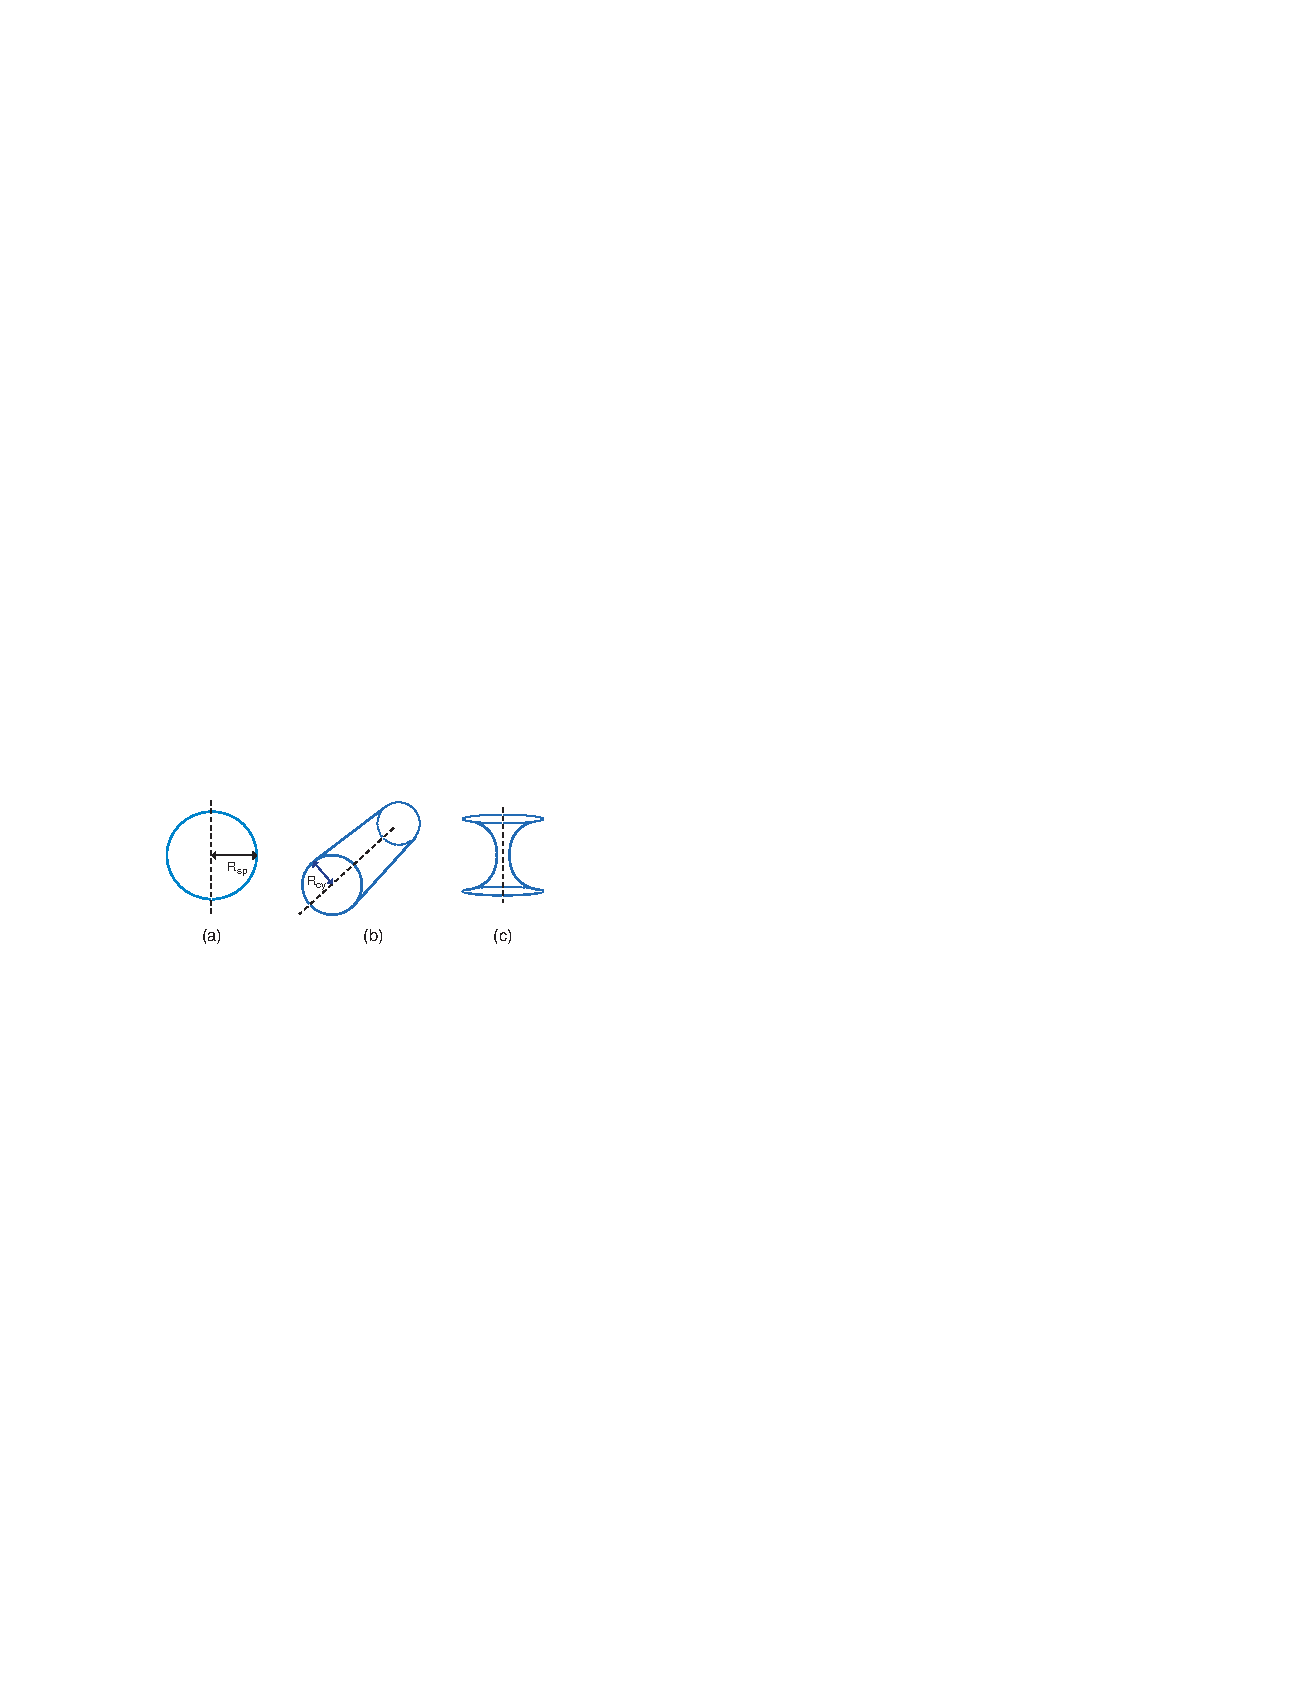
\includegraphics[width=\columnwidth]{\MemTB/Pics/simpleMembraneShapes}
\caption{
شکل‌های ساده‌ی غشا که در تمام نقاط روی سطح انحنای میانگین ثابتی دارند. شکل الف، کُره‌ای به شعاع 
$R_{sp}$
با انحنای میانگین 
$M=\pm 1/R_{sp}$
ب، استوانه‌ای با شعاع 
$R_{cy}$
با انحنای میانگین
$M=\pm 1/2R_{cy}$
و در نهایت ج، کتانوید با انحنای میانگین صفر. علامت انحنای میانگین برای کُره و استوانه به این بستگی دارد که محیط بیرون، سیال خارج از غشا تعریف شود یا سیال داخل.
}
\label{fig:simpleMembraneShapes}
\end{center}
\end{figure}
به طور عمومی انحنای میانگین یک کمیت موضعی است و در نقاط مختلف روی سطح غشا تغییر می‌کند. اما برخی اَشکال ساده در تمامی نقاط روی سطح خود یک مقدار ثابت انحنای میان‌گین دارند. برای مثال انحنای میانگین یک غشای تخت صفر است. برای مثال‌های بیشتر با شکل 
\ref{fig:simpleMembraneShapes}
توجه کنید. انحنای میانگین یک کُره با شعاع
$R_{sp}$
برابر با 
$C=1/R_{sp}$
هنگامی که لایه‌ی خارجی آن با محیط بیرون غشا در ارتباط است و 
$C=-1/R_{sp}$
زمانی که لایه‌ی داخلی آن با محیط بیرون در ارتباط است. همچنین استوانه‌‌ای با شعاع 
$R_{cy}$
دارای انحنای میانگین
$C=\pm1/2R_{cy}$
که علامت آن تابع تعریف جهت بردار عمود خواهد بود. یک شکل ساده‌ی جالب، کتانوید\LTRfootnote{catanoid} 
 است که تمام نقاط روی سطح آن از نقاط زین اسبی تشکیل شده و در نتیجه انحنای میانگین همه جا انحنای میانگین آن صفر است.





 
 
 
 
 




\subsection{
خمش ذاتی
}
تا به اینجا فرض شده که تک لایه‌های تشکیل دهنده‌ی غشا تمایلی به خم شدن در جهت مشخصی ندارند. شکل تعادلی موضعی چنین غشایی یک سطح تخت خواهد بود. کمتر غشایی در طبیعت با چنین تقارنی مشاهده می‌شود ولی دلیل مطالعه‌ی چنین سیستم از نظر مدل‌سازی بسیار پر بهره است چرا که تمام ویژگی‌های الاستیک آن توسط پارامتر سختی خمش
$\kappa$
تعیین می‌شود که مقیاس خوبی برای انرژی یک غشاست. برای غشاهای فسفولیپیدی در دمای اتاق مرتبه‌ی انرژی سختی خمش حدود
$10^{19}J$,
یا
$20k_BT$
است. سختی خمش برای غشاهای از جنس دیگر ممکن است تا حدود یک مرتبه‌ی بزرگی متفاوت باشد. به دلیل اختلاف در ترکیبات تک لایه‌های سازنده‌ی غشاهای زیستی
\cite{Meer2008},
 غشاهای دولایه معمولا نامتقارن هستند. معروف‌ترین مثال غشاهای تشکیل شده از گنگلیوساید 
$GM1$\LTRfootnote{ganglioside GM1}  
است که از نوع گلایکولیپید‌هاست\LTRfootnote{glycolopids}  
و در غشاهای سلول‌های عصبی پستانداران به طور فراوان یافت می‌شود. 
$GM1$
نقش لنگر را برای مواد سمی، باکتری‌ها، و ویروس‌ها بازی می‌کند
\cite{Ewers2010}.
نحوه‌ی تغییر خمش موضعی با تغییر غلظت 
$GM1$
به طور مفصل به شکل تجربی
\cite{Bhatia2018, Raktim2018}
و هم به شکل شبیه‌سازی
\cite{Raktim2018, Sreekumari2018}
مطالعه شده‌است. همچنین جهت‌گیری پروتئین‌های درون غشا، چسبیدن پروتئین‌های محیط بر سطح غشا معمولا خمش را تغییر می‌دهد. در نتیجه اگر ذرات زیادی به سطح غشا بچسبند، خمش ذاتی در سطح غشا،
$C_0$
، ایجاد خواهد شد
\cite{Lipowsky2002}
که تابع تعداد ذراتی‌ است که به تک‌لایه‌های مختلف غشا متصل شده باشند
\cite{Breidenich2000}.
 مقدار خمش ذاتی بسیار متغییر است و از مقیاس موضعی 
$1/10nm$
تا مقیاس خود غشا
$1/50\mu m$
گزارش شده است.


\subsection{
نظریه‌ی مدل خمش ذاتی
\label{sec:spontaneousCurvatureModel}
}
در این بخش به بنا کردن چهارچوب نظریه‌ای پرداخته می‌شود که نقش کلیدی در فهم شکل‌های غشا‌های غول‌آسا داشته است. این نظریه بر اساس انرژی الاستیک خمش غشا ایجاد شده‌است. همچنین در این نظریه حل‌شوندگی بسیار کم مولکول‌های لیپیدی و تاثیر اختلاف فشار اسمزی به شکل قید روی سطح و حجم غشا در نظر گرفته شده است. درواقع جذابیت این نظریه در توصیف تبادل بین انرژی‌هایی است با منشا موضعی و سراسری. از طرفی شکل انحنای غشا بر اساس انرژی‌های ناشی از خمش‌های موضعی (خمش میانگین و خمش گاووسی) تعیین می‌شود و از طرف دیگر با فرض اینکه غشا تغییر توپولوژیکی نداشته باشد (با غشای دیگری جوش نخورد، تکه‌ای از غشا به شکل جوانه از آن جدا نشود، یا حفره‌ای در آن ایجاد نشود) سطح و حجم ثابتی خواهد داشت که بر شکل نهایی که غشا می‌تواند به خود بگیرد تاثیر بسیار مشخصی دارد. ارتباط میان پدیده‌های موضعی و سراسری با دو کمیت به نام تنش مکانیکی\LTRfootnote{mechanical tension}  
$\gamma_{ten}$
و اختلاف فشار
$\Delta P$
برقرار می‌شود.

نظریه‌ی مدل خمش ذاتی\LTRfootnote{spontaneous curvature model}  
یک غشا را با دو مشخصه‌ی هندسی، سطح غشا 
$A$
و حجم آن 
$V$
، به همراه دو مشخصه‌ی مادی\LTRfootnote{material property}  
سختی خمش غشا
$\kappa$
و خمش ذاتی 
$C_0$
آن توصیف می‌کند. مدل خمش ذاتی بر اساس انرژی خمش بر حسب توان‌های خمش‌های اصلی پایه‌گزاری شده و تا زمانی که خمش نسبت به عکس ضخامت غشا کوچک باشند پابرجاست.
انرژی انحنای غشایی که شکل 
$S$
را دارد 
$\mathcal{E}_{cu}\{S\}$
است که بر حسب انتگرال سطحی چگالی موضعی انرژی 
$\varepsilon_{cu}(S)$
تعریف می‌شود،
\begin{equation}
\mathcal{E}_{cu}\{S\}=\int dA~\varepsilon_{cu}(S).
\end{equation}
فرض می‌کنیم چگالی انرژی موضعی تنها تابع خمش‌های اصلی 
$C_1$
و
$C_2$
است. همچنین اگر در هر نقطه بر روی سطح غشا دستگاه مختصات را 
$\pi/2$
در جهات بردار عمود برسطح دوارن دهیم، انرژی خمش نباید تغییر کند،
$\varepsilon_{cu}(C_1,C_2)=\varepsilon_{cu}(C_2,C_1)$.
بسط انرژی تا جمله‌ی توان دوم به شکل حدی با معادله‌ی زیر برابر خواهد بود،
\begin{equation}
\varepsilon_{cu}(C_1,C_2)\approx a_0+a_1(C_1+C_2)+a_2(C_1^2+C_2^2) + a_3 C_1C2.
\end{equation}
این بسط را می‌توان بر حسب خمش میانگین و خمش ذاتی به شکل زیر باز نویسی کرد،
\begin{equation}
\varepsilon_{cu}\approx 2\kappa(M-C_0)^2+\kappa_GG.
\end{equation}
با جایگذاری در انتگرال سطحی شکل انرژی انحنای هلفریش
\LTRfootnote{Helfrich}
\cite{Helfrich1973}
بدست می‌آید،
\begin{equation}
E_{cu}=\int dA\left[\frac{1}{2}\kappa(C_1+C_2-2C_0)^2+\kappa_GC_1C_2\right],
\label{eq:HelfrichCurvatureEnergy}
\end{equation}
که به دو انتگرال انرژی خمش 
\begin{equation}
E_{b}=\frac{1}{2}\kappa\int dA (C_1+C_2-2C_0)^2
\label{eq:HelfrichBendingEnergy}
\end{equation}
و انرژی خمش گاووسی
\begin{equation}
E_{G}=\kappa_G\int dA C_1C_2
\label{eq:HelfrichGaussianEnergy}
\end{equation}
تقسیم می‌شود.
در صورتی که غشا هندسه‌ی بسته داشته باشد و هیچ لبه‌ی آزادی در آن نباشد (مثلا یک شکل کُروی داشته باشد و به شکل یک صفحه‌ی آزاد در محیط نباشد) قضیه‌ی گاووس-بونت\LTRfootnote{Gauss-Bonnet theorem}
\cite{NelsonBook2004}
در هندسه‌ی دیفرانیسیلی جواب انتگرال معادله‌ی
\ref{eq:HelfrichGaussianEnergy}
 تابع مشخصه‌ی اویلری رویه\LTRfootnote{Euler characteristic of the surface}
 یا جینوس\LTRfootnote{genus}
خواهد بود.
 \begin{equation}
E_{G}=\kappa_G\int dA C_1C_2=2\pi\kappa_G(2-2g).
\label{eq:GaussianBonnet}
\end{equation}
 
 جینوس سطح تعداد سوراخ‌هایا تعداد دسته‌های یک شکل را می‌شمارد.
مثلا یک کُره هیچ سوراخ یا دسته‌ای ندارد و جینوس آن صفر است. در صورتی که یک شکل چنبره\LTRfootnote{toroid}
یک سوراخ یا دسته دارد و جینوس آن یک است
$g=1$
. همچنین رویه‌ای که سطح یک لیوان دسته‌دار را می‌پوشاند جینوس برابر با یک خواهد داشت (به مثال‌های شکل 
\ref{fig:genus012}
توجه کنید).
\begin{figure}[t]
\begin{center}
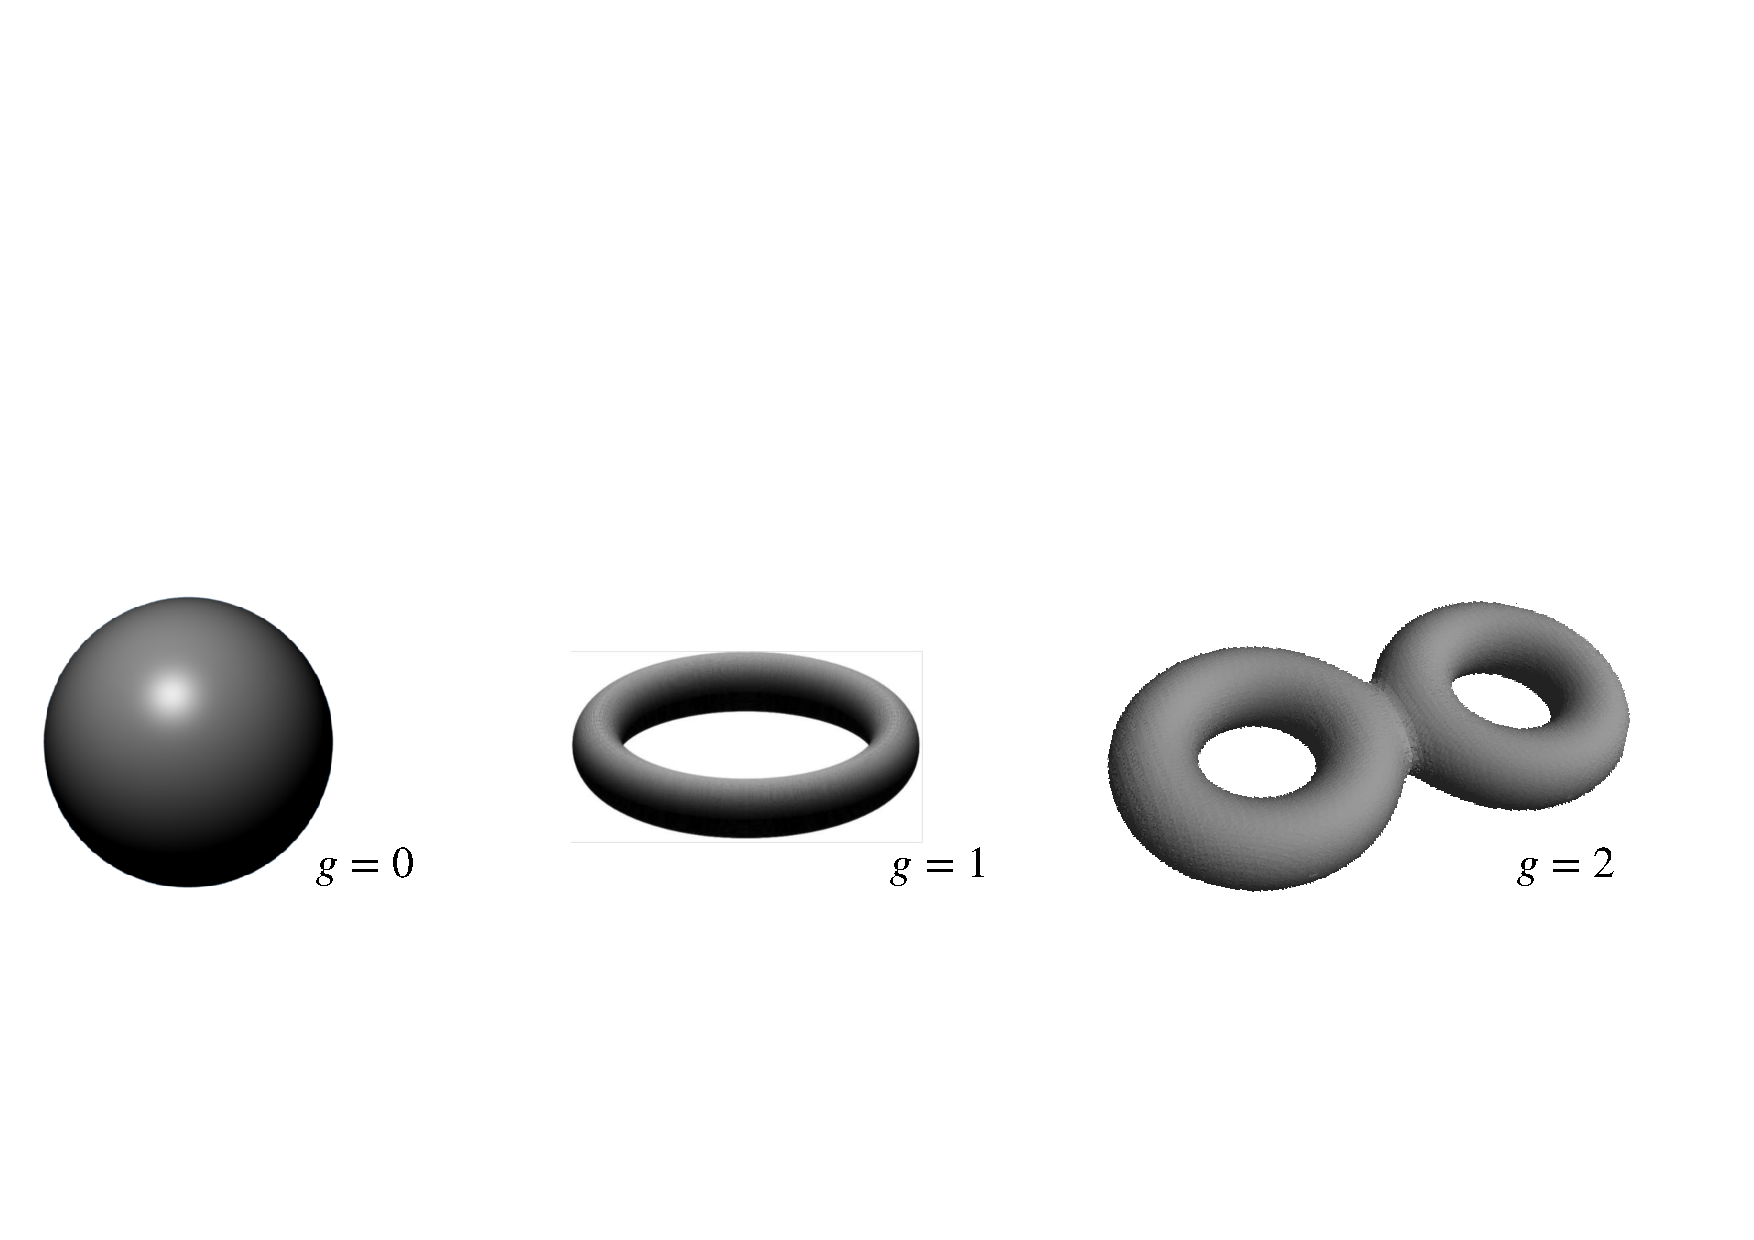
\includegraphics[width=\columnwidth]{\MemTB/Pics/genus}
\caption{
به ترتیب از چپ به راست یک کُره، چنبره، و دو چنبره متصل به هم را مشاهده می‌کند که به ترتیب شکلی با 
$0$, $1$,
 و 
$2$
سوراخ/دسته که همچنین مقدار جینوس این سطوح را تعیین می‌کند.
}
\label{fig:genus012}
\end{center}
\end{figure}
برای مثال انرژی انحنای یک کُره به شعاع
$R$
را با استفاده از معادلات
\ref{eq:HelfrichBendingEnergy}
و
\ref{eq:HelfrichGaussianEnergy}
محاسبه می‌کنیم. با فرض اینکه بردار عمود بر سطح کره در جهت خارج کُره تعریف شده باشد، از انجایی که شعاع‌ کره در تمام نقاط سطح آن ثابت است خمش در سراسر سطح با یک مقدار
$C_1=C_2=1/R$
تعیین می‌شود. تنها فرض باقی مانده تعیین خمش ذاتی شکل است. در صورتی که فرض شود حالت تعادلی رویه‌ای که کُره را تشکیل داده سطح تخت باشد
$C_0=0$
انرژی آن
 \begin{equation}
 \begin{aligned}
E_{b}&=\frac{1}{2}\kappa\int R^2d\Omega (\frac{2}{R}-0)^2=8\pi\kappa\\
E_{G}&=\kappa_G\int R^2d\Omega \frac{1}{R^2}=4\pi\kappa_G=2\pi\kappa_G(2-2g)=2\pi\kappa_G(2-0) \\
E_{cu}&=8\pi\kappa+4\pi\kappa_G.
\end{aligned}
\end{equation}
در صورتی که خمش ذاتی آن،
$C_0=1/R$
باشد انرژی انحنای آن
 \begin{equation}
 \begin{aligned}
E_{b}&=\frac{1}{2}\kappa\int R^2d\Omega (\frac{2}{R}-\frac{2}{R})^2=0\\
E_{G}&=2\pi\kappa_G(2-2g)=4\pi\kappa_G \\
E_{cu}&=4\pi\kappa_G
\end{aligned}
\end{equation}
است. توجه کنید که انرژی انحنای محاسبه شده تابع شعاع کُره نیست. به طور عمومی انرژی محاسبه شده با مدل خمش ذاتی از مقیاس شکل مستقل است. در نتیجه مدول خمشی
$\kappa$
نیز تابع مقیاس سیستم نخواهد بود. این مفهوم بسیار متفاوت از تعاریف رایج از مدول خمشی برای پلیمر‌هاست و باید توجه ویژه‌ای به این نکته بشود. از آنجایی که در مطالعه‌ی شکل غشا معمولا اختلاف انرژی بین اشکال اهمیت دارد و (به خصوص برای محاسبه‌ی نیرو) تا زمانی که غشا تغییر توپولوژیکی نداشته باشد، از محاسبه‌ی مقدار ثابت انرژی خمش گاووسی چشم پوشی می‌شود. 







































\section{
انرژی کشش الاستیک
}
%\setRL
%\pagenumbering{arabic} 

بعضی غشاها تنها از یک غشای دو‌-لایه‌ی لیپیدی تشکیل نشده‌اند. مانند غشای هسته‌ی سلول‌های پستانداران که معمولا از دو غشای لیپیدی دو لایه متصل به یک شبکه‌ی پلیمری دو بعدی الاستیک تشکیل شده‌است. در این بخش به مدل‌سازی انرژی شبکه‌های پلیمری الاستیک می‌پردازیم.
%\subsection{
%انرژی کشش در سطح
%}
اگر فرض کنیم جابجایی روی یک عنصر سطحی حاصل از کشیده‌ یا فشرده شدن سطح با بردار 
$u$
توصیف شود، با فرض خطی بودن عکس العمل ماده، انرژی پتانسیل حاصل از تغییر شکل سطح را می‌توان با معادله‌ی زیر بررسی کنیم،
\begin{equation}
E_{stretching}=\frac{1}{2}Y_{2D}A\varepsilon^2.
\end{equation}
که اینجا 
$Y_2D$
مدول دو بعدی یانگ،
$A$
سطح عنصر در حالت کشیده نشده، و
$\varepsilon$
تانسور کرنش است. تانسور کرنش برای سطح دو بعدی به شکل زیر تعریف می‌شود:
\begin{equation}
\varepsilon_{ij} = \frac{1}{2}(u_{ij}+u_{ji})
\end{equation}


در نظریه‌ی الاستیک سطح هر تغییر شکل با یک میدان بردار جابجایی 
$u(r)=(u_1,u_2)$
نشان داده می‌شود نقطه‌ی 
$r(x,y)$
را به نقطه‌ی 
$r+u$
نگاشت می‌کند. اگر در شبکه نقص وجود نداشته باشد این نگاشت یک به یک خواهد بود. در صورتی که فرض کنیم که ماده مورد مطالعه یکنواخت و همسانگرد است، برای جابجایی‌های کوچک (رژیم خطی) قانون هوک را به شکل توان دوم تانسور کرنش\LTRfootnote{Cauchy, 1822; Lam ́e, 1852}
نوشت،
\begin{equation}
E_s=\frac{1}{2}\int d^2r(2\mu u_{ij}^2+\lambda u_{kk}^2).
\label{eq:energylame}
\end{equation}
در اینجا $\lambda$
و $\mu$
ثابت‌های لم\LTRfootnote{Lamé Coefficients}
است. ما می‌دانیم که تانسور کرنش به شکل زیر تعریف می‌شود،
\begin{equation}
u_{ij}=\frac{1}{2}(\partial_i u_j+\partial_j u_i+\partial_i u_k\partial_j u_k).
\end{equation}
اما برای جابجایی کوچک از جمله‌ی غیر خطی صرف نظر می‌کنیم و تانسور کرنش را به این شکل تعریف می‌کنیم،
\begin{equation}
u_{ij}=\frac{1}{2}(\partial_i u_j+\partial_j u_i).
\label{eq:simplestrain}
\end{equation}
می‌توانیم  از انرژی کششی گرادیان بگیریم و مقدار کمینه‌ی آن را بررسی کنیم، در نتیجه،
\begin{equation}
\begin{aligned}
&\partial_i\sigma_{ij}=0\\
&\sigma_{ij}=2\mu u_{ij}+\lambda u_{kk}\delta_{ij}.
\label{eq:stress}
\end{aligned}
\end{equation}
در این معادله 
$\sigma_{ij}$
تانسور تنش است. معادله‌ی 
\ref{eq:stress}
را به تنهایی می‌توان حل کرد ولی از آنجایی که دیورژانس تنش صفر است معمول است که این معادله را به شکل یک پتانسیل اسکالر بنویسیم،
\begin{equation}
\sigma_{xx}=\frac{\partial^2\chi}{\partial y^2},\quad\sigma_{yy}=\frac{\partial^2\chi}{\partial x^2},\quad\sigma_{xy}=\frac{\partial^2\chi}{\partial_x\partial_y}.
\end{equation}
انتخاب‌های خیلی زیادی می‌توانند معادله‌ی بالا را ارضاء خواهد کرد، ولی جواب‌هایی که به لحاظ فیزیک قابل قبول هستند باید بتوانند رابطه‌ی بین میدان جابجایی و 
$\chi$
را رعایت کنند،
\begin{equation}
\begin{aligned}
\frac{1}{2}(\partial_iu_j+\partial_ju_i)&=u_{ij}\\
&=\frac{1+\nu}{Y}\sigma_{ij}-\frac{\nu}{Y}\sigma_{ll}\sigma_{ij}\\
&=\frac{1+\nu}{Y}\epsilon_{im}\epsilon_{jn}\partial_{m}\partial_{n}\chi-\frac{\nu}{Y}\nabla^2\chi\delta_{ij}.
\label{eq:constraint}
\end{aligned}
\end{equation}
در اینجا $Y$
و $\nu$
به ترتیب مدول ۲ بعدی یانگ\LTRfootnote{2D Young Modulus}
 و نسبت پواسون\LTRfootnote{Poisson ratio}
است که بر حسب ضرایب لم به شکل زیر بیان می‌شوند،
\begin{equation}
\begin{aligned}
Y&=\frac{4\mu(\mu+\lambda)}{2\mu+\lambda}\\
\nu&=\frac{\lambda}{2\mu+\lambda}.
\label{eq:younglame}
\end{aligned}
\end{equation}

 
 
 
 
 
 













\clearpage
\clearpage
\chapter{
\centering{
افت و خیز روی سطح کره
}
}
\setRL
\clearpage
\def \MemFluc {\Mempath /MembraneFluc}

\section{
چکیده
}
در این فصل با استفاده از روش تحلیل افت و خیز، انرژی پوسته‌های نازک در حال نوسان را بررسی می‌کنیم. مطالعه‌ی افت و خیز‌های سطحی اطلاعات خوبی راجع به فیزیک حاکم بر سیستم در اختیار مشاهده‌گر قرار می‌دهد. همچنین با استفاده از قضیه‌ی هم پاری انرژی می‌توان شدت‌ مد‌های نوسانی مختلف را پیش‌بینی کرد و حتی مقیاس زمانی نوسانات را تخمین زد.

\section{
مقدمه
}




در فصول قبل نحوه‌ی محاسبه‌ی انرژی انحنا و کششی سطوح دو بعدی را مطالعه کردیم. حال فرض می‌کنیم که یک رویه‌ی دو بعدی با هندسه‌ی بسته در اختیار داریم که حجم کاهیده‌ی آن نزدیک به یک کُره است. سطح این رویه به علت اُفت و خیز ترمودینامیکی محیط دائم در حال تغییر است. در صورتی که یک لحظه زمان را متوقف کنیم، رویه‌ای خواهیم داشت که سطح آن پُر از برآمدگی و فرورفتگی در مکان‌های تصادفی است. اگر فرض کنیم اطلاعات مکانی تمام نقاط روی سطح را در اختیار داشته باشیم چطور می‌توانیم انرژی انحنا یا انرژی کشش این سطح را اندازه‌گیری کنیم؟ 

\begin{figure}[h]
\begin{center}
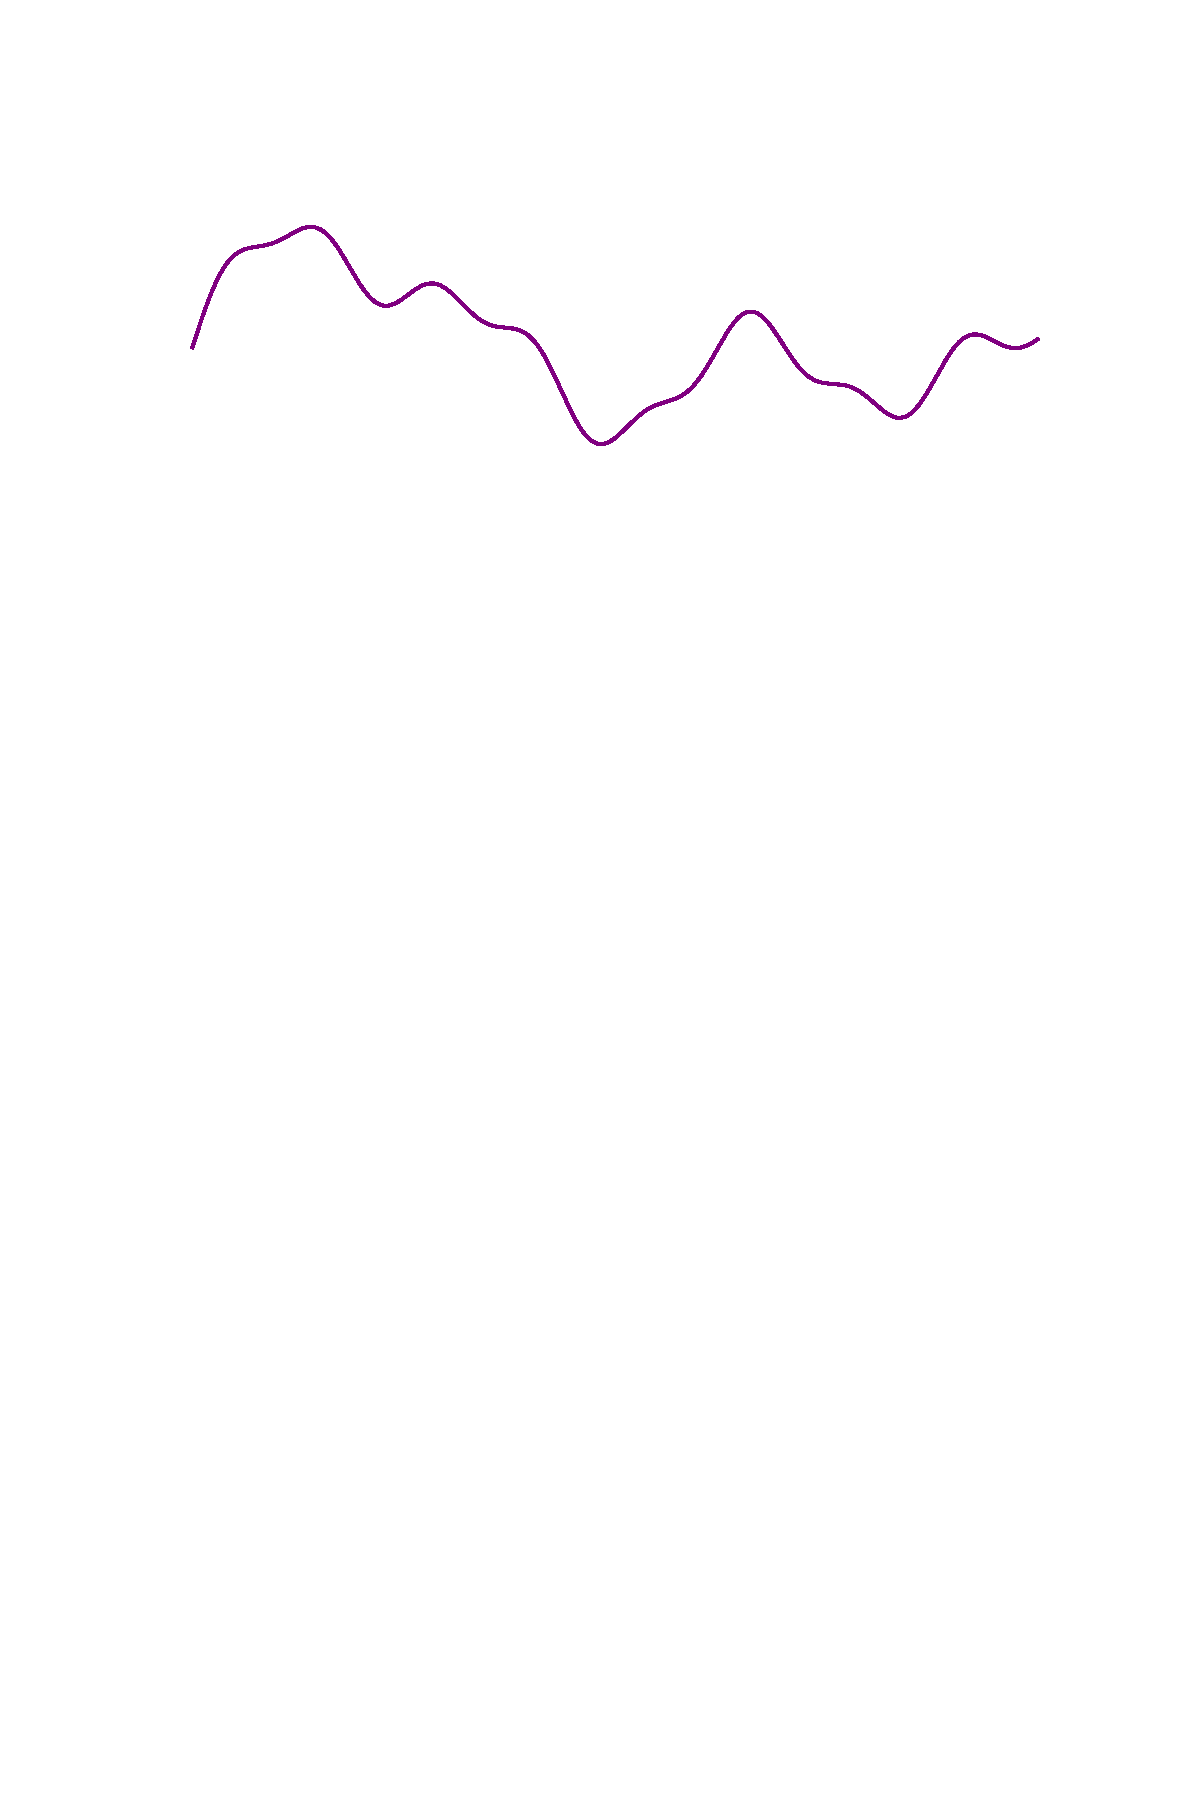
\includegraphics[width=6in]{\MemFluc /Pics/signal_1}
\caption{
 یک ریسمان که در حال افت و خیز در فضای ۲ بعدی. دو انتهای ریسمان ثابت است.
}
\label{fig:flucString1}
\end{center}
\end{figure}


حالا فرض کنیم که مسئله‌ی ساده‌تری را مطالعه می‌کنیم. فرض کنیم که به جای رویه، یک ریسمان در اختیار داریم که دو سر آن ثابت است و ریسمان  در یک فضای ۲ بعدی  در حال افت و خیز است. در شکل 
\ref{fig:flucString1}
چیدمان این ریسمان در زمان تصادفی‌ رسم شده‌است.
\begin{figure}[h]
\begin{center}
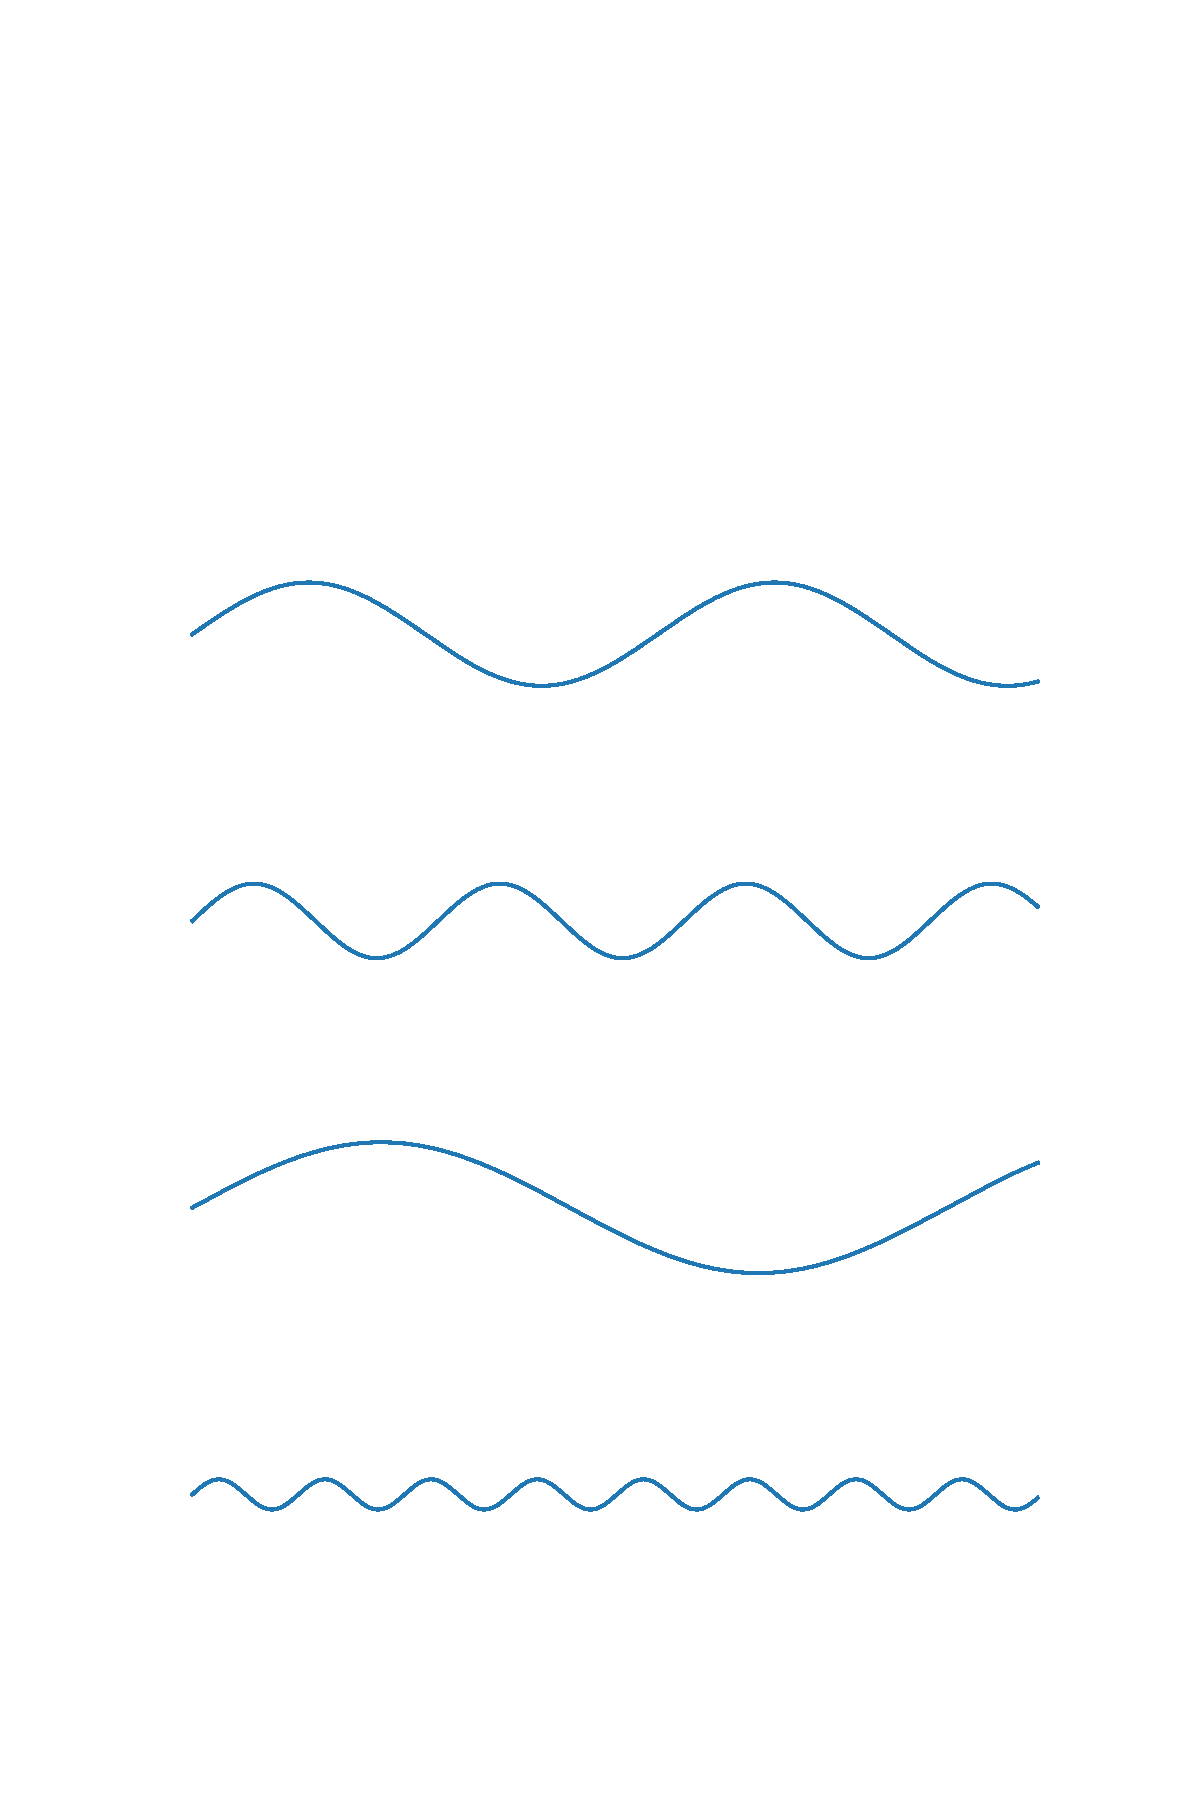
\includegraphics[width=4in]{\MemFluc /Pics/signal_2}
\caption{
مُدهای نرمال تشکیل دهنده‌ی شکل
\ref{fig:flucString1}
را نشان می‌دهد. شکل
\ref{fig:flucString1}
از چهار مُد نرمال با فرکانس و شد‌ت مختلف ساخته شده‌است. 
}
\label{fig:flucString2}
\end{center}
\end{figure}
در صورتی که لازم باشد اطلاعات ساده‌ای مانند انرژی جنبشی یا انرژی پتانسیل این ریسمان محاسبه شود، با فرض اینکه اصل برهم نهی بر قرار است، کافی است که مُدهای نرمال این ریسمان را پیدا کنیم. مُدهای نرمال این ریسمان با توابع مثلثاتی تعریف می‌شوند. با محاسبه‌ی مجموع انرژی جنبشی یا پتانیسل مُدهای تشکیل دهنده‌ی این شکل می‌توانیم انرژی کلی جنبشی یا پتانسیل این ریسمان را محاسبه کنیم. در شکل
\ref{fig:flucString2}
مد‌های تشیل دهنده‌ی این ریسمان رسم شده‌است.


.
 
 
 
 
 
 
 
 
 
 
 

\section{
محاسبه‌ی اندازه افت و خیز روی کره
\label{sec:bendingFluctuations}
}
\input{\MemFluc/spherical}

\section{
افت و خیز مساحت و حجم کُره
}

 کُره‌ بر اساس تعریف آن حجم کاهیده‌ی 
 $\nu=1$
 دارد. غشا با حجم کاهیده‌ی واحد نمی‌تواند افت و خیز کند، زیراکه برای افت و خیز مساحت آن باید کمی بیشتر از مساحت کُره با همان حجم باشد. می‌توانیم مساحت شکلی که در حال افت و خیز است را به شکل زیر محاسبه کنیم. از بخش قبل می‌دانیم که
\begin{equation}
dA=r_{0}^2(1+g^2+\frac{1}{2}g\mathcal{L}^2g)d\Omega
\label{eq:areaPatchDifferential}
\end{equation}
 و با انتگرال گیری روی تمام زوایای فضایی،
 \begin{equation}
\begin{aligned}
A&=\int dA=r_{0}^2\int(1+g^2+\frac{1}{2}g\mathcal{L}^2g)d\Omega\\
&=r_{0}^2(4\pi+\sum_{\ell}|u_{\ell,m}|^2[1+\frac{1}{2}\ell(\ell+1)])
\label{eq:AreaGL}
\end{aligned}
\end{equation}
 حجم غشای در حال افت و خیز نیز به همین ترتیب قابل محاسبه‌است. با انتگرال گیری بر روی تمام زوایای فضای حجم غشا را محاسبه می‌کنیم،
\begin{equation}
\begin{aligned}
V&=\int dV=\frac{1}{3}\int r^3d\Omega\\
&=\frac{1}{3}r_{0}^3\int(1+g)^3d\Omega=\frac{1}{3}r_{0}^3\int1+3g+3g^2d\Omega\\
&=\frac{1}{3}r_{0}^3(4\pi+3\sum_{\ell}|u_{\ell,m}|^2)
\label{eq:VolumeGL}
\end{aligned}
\end{equation}
حالا با استفاده از معادلات
\ref{eq:AreaGL}
و
\ref{eq:VolumeGL}
و جایگذاری در معادله‌ی
\ref{eq:reducedVolume}
حجم کاهیده شکل در حال افت و خیز  را محاسبه می‌کنیم،
\begin{equation}
\begin{aligned}
\nu=\frac{\sqrt{4\pi}(4\pi+\sum|u_{\ell,m}|^2)}{(4\pi+3\sum|u_{\ell,m}|^2[1+\frac{1}{2}\ell(\ell+1)])^{3/2}}
\label{eq:nuUndulated}
\end{aligned}
\end{equation}
%با فرض اینکه ضریب سختی خمش یک غشا حدود
%$\kappa=20k_BT$
%است، با جمع روی مُدها می‌توان حجم کاهیده‌ی لازم را حدود
%$\nu\approx0.9626$
%تخمین زد.


\section{
افت و خیز سطح کُره‌ی جامد
}
کانون توجه این رساله بررسی اُفت و خیز سطح غشا‌های جامد (مانند شبکه‌ی پلیمری گلبول‌های قرمز) و پوسته‌های الاستیکی

نیست. اما جهت تکمیل مطالعه‌ی افت و خیز، لازم می‌دانم که به شکل شدت افت و خیز سطح پوسته‌ی کروی الاستیک به شعاع
$R$
، مدول یانگ دو بعدی
$Y_{2d}$
، خمش ذاتی 
$r_s=R$
، سختی خمش
$\kappa$
، و تحت اختلاف فشار 
$p$
در دمای 
$k_BT$
را معرفی کنم. افت و خیز چنین سطحی تا مرتبه‌ی دوم به شکل 
\begin{equation}
\langle|u_{\ell,m}|^2\rangle=\frac{k_BT}{\kappa(\ell+2)^2(\ell-1)^2-pR^3\left[1+\frac{1}{2}\ell(\ell+1)\right]+R^2\frac{Y_{2D}}{1+\frac{Y_{2D}}{2\mu(\ell^2+\ell-2)}}}
\label{eq:ulmSolid}
\end{equation}


تعریف می‌شود. و تعریف مدول یانگ دو بعدی بر حسب ضرایب لمه
\LTRfootnote{lam\'e coefficients}
$\lambda,\mu$
به شکل
\begin{equation}
Y_{2D}=\frac{4\mu(\mu+\lambda)}{2\mu+\lambda}
\label{eq:youngLame}
\end{equation}

است. همچنین می‌توان معادله‌ی
\ref{eq:ulmSolid}
را برای ماده‌ای که دارای تنش بُرشی 
$\mu=3Y_{2D}/8$
باشد (مثلا موادی که اتصالاتشان شبکه‌ی مثلثی تشکیل می‌دهد) به شکل زیر تقریب زد،
\begin{equation}
\langle|u_{\ell,m}|^2\rangle=\frac{k_BT}{\kappa(\ell+2)^2(\ell-1)^2-pR^3\left[1+\frac{1}{2}\ell(\ell+1)\right]+Y_{2D}R^2\frac{3(\ell^2+\ell-2)}{3(\ell^2+\ell)-2}}
\label{eq:ulmSolidTri}
\end{equation}
جزئیات محاسبات بخش خمش طبق محاسبات ارائه شده در این رساله‌است و محاسبات مربوط به اثر فشار و خاصیت الاستیکی سطح با جزئیات کامل در مرجع
\cite{gomppernelson2012}
یافت می‌شود.


\section{
افت و خیز بر روی مدارهای
$\theta$
}




در بخش‌های قبل اطلاعات دامنه‌ی افت و خیز کره (مد‌های هماهنگ کروی بر رویه‌ی ۲ بعدی در فضای ۳ بعدیی) را محاسبه‌ کردیم. برای اندازه‌گیری شدت دامنه‌ی مد‌های بر برش‌های در راستای 
$\theta$
(مد‌های هماهنگ بر حلقه‌ی ۱ بعدی در فضای ۲ بعدی) کافی‌است که  تصویر همه‌ی مد‌ها را در بُرش مورد نظر جمع بزنیم
\cite{Prost2004}
.
\begin{equation}
\langle|u_m(\theta)|^2\rangle=\sum_{\ell=m}^{\ell=\ell_{max}}\frac{2\ell+1}{4\pi}\frac{(\ell-|m|)!}{(\ell+|m|)!}\left(P_\ell^{|m|}(\cos(\theta))\right)^2\langle|u_{\ell,m}|^2\rangle
\label{eq:3Dto2Dsum}
\end{equation}


\section{
محاسبه‌ی نیروی عمود بر سطح غشا
\label{sec:NormalForceDerivation}}
مشابه به روش انجام شده در مرجع 
\cite{milnersafranPRA1987}
انحنای سطحی به خمش ذاتی صفر به شکل زیر تعریف می‌شود،
\begin{equation}
H= C_1+C_2=\vec\nabla\cdot\vec n=\frac{2}{r}(1+\frac{r_0}{2r}{\cal L}^2g).
\end{equation}
برای 
$g$
های کوچک وارون شعاع را می‌توان با 
$1/r\approx\frac{1}{r_0}(1-g)$
تخمین زد. از آنجایی که چگالی نیرو بر روی سطح غشا به شکل 
$-\kappa\nabla^2H$
تعریف می‌شود، برای بدست آوردن رابطه‌ی مناسب کافی است که لاپلاسین جمله‌ی بالا را محاسبه کنیم،
\begin{equation}
\begin{aligned}
\nabla^2H=\left[\frac{1}{r^2}\frac{\partial}{\partial r}\left(r^2\frac{\partial}{\partial r}\right)-\frac{1}{r^2}{\cal L}^2\right]\left(\frac{2}{r}(1+\frac{r_0}{2r}{\cal L}^2g)\right).
\label{eq:forceDensityDeriv}
\end{aligned}
\end{equation}
مشتق‌های شعاعی جمله‌ی بالا به شکل نهایی زیر ساده خواهند شد،
\begin{equation}
\begin{aligned}
\frac{1}{r^2}\frac{\partial}{\partial r}\left(r^2\frac{\partial}{\partial r}\left(\frac{2}{r}(1+\frac{r_0}{2r}{\cal L}^2g)\right)\right)\\
=\frac{-2}{r^2}\frac{\partial}{\partial r}\left(1+\frac{r_0}{r}{\cal L}^2g\right)\\
=\frac{2r_0}{r^4}{\cal L}^2g.
\end{aligned}
\end{equation}
مشتقات زاویه‌ای نیز به صورت زیر ساده می‌شوند،
\begin{equation}
\begin{aligned}
-\frac{1}{r^2}{\cal L}^2\left(\frac{2}{r}(1+\frac{r_0}{2r}{\cal L}^2g)\right)\\
=-\frac{r_0}{r^4}{\cal L}^2({\cal L}^2g).
\end{aligned}
\end{equation}
با جاگذاری مشتقات، تعریف 
\ref{eq:forceDensityDeriv}
به شکل ساده‌تر زیر بازنویسی می‌شود،
\begin{equation}
\begin{aligned}
\nabla^2H=\frac{r_0}{r^4}\left(2{\cal L}^2g-{\cal L}^2({\cal L}^2g)\right).
\end{aligned}
\end{equation}
در نتیجه چگالی نیرو در هر زاویه‌ای بر روی سطح غشا به این صورت خواهد بود،
\begin{equation}
\begin{aligned}
F(\theta,\phi)&=-\int\kappa\nabla^2H\frac{dA}{d\Omega}\\
&=\kappa\frac{r_0}{r^4}\left(2{\cal L}^2g-{\cal L}^2({\cal L}^2g)\right)r^2\left(1+\frac{r_0^2}{2r^2}g{\cal L}^2g\right)\\
&=\frac{\kappa r_0}{r^2}\left(2{\cal L}^2g-{\cal L}^2({\cal L}^2g)\right) + {\cal O}(g^3)\\
\end{aligned}
\end{equation}
با پیاده‌سازی تبدیل فوریه کروی 
$F(\theta,\phi)$
نیروی ناشی از هر مد را می‌توان محاسبه کرد،
\begin{equation}
\begin{aligned}
f_{\ell,m}&=\int F(\theta,\phi)Y_{\ell,m}^*(\theta,\phi)d\Omega\\
f_{\ell,m}&=-\frac{\kappa}{r_0}u_{\ell,m}(\ell+2)(\ell+1)\ell(\ell-1)
\label{eq:normal_force_lm}
\end{aligned}
\end{equation}


















\section{
دینامیک و مقیاس زمانی
}

در این بخش به محاسبه‌ی زمان دوره‌ی تناوبی بسامد نوسان‌‌های هماهنگ‌های کروی برای یک غشای سیال‌گون می‌پردازیم. 
در بخش 
\ref{sec:bendingFluctuations}
انرژی انحنای یک غشای بر اساس مُدهای نرمال آن (هماهنگ‌های کُروی) محاسبه شد. معادله‌ی لاگرانژ، دینامیک درجه‌های آزادی را به تغییرات انرژی درجات آزادی، 
$q$
مرتبط می‌کند،

\begin{equation}
\frac{d}{dt}\left(\frac{\partial K}{\partial \dot q}\right)=-\frac{\partial U}{\partial q}.
\label{eq:LagrangeEquation}
\end{equation}
در معادله‌ی فوق
$K$
انرژی جنبشی،
$U$
انرژی پتانسیل سیستم مورد مطالعه‌است. این معادله مستقل از شکل معادله‌ی دینامیک سیستم بر قرار است. در صورتی که غشا در محیط خلا در حال نوسان باشد، معادله‌ی حرکت سیستم توسط معادله‌ی نیوتن تعیین می‌شود. در صورتی که غشا در محیط سیال در حال نوسان باشد، معادله‌ی حرکت با حل معادله‌ی ناویر-استوکس
\LTRfootnote{Navier-Stokes }
تعیین می‌شود. برای غشایی که در خلا حرکت می‌کند، انرژی جنبشی آن به سادگی با جمع روی انرژی جنبشی تکه‌های جرمی کوچک برای سطح آن محاسبه می‌شود،
\begin{equation}
\begin{aligned}
K&=\frac{1}{2}\rho_m\int\d\Omega~\dot r^2(\theta,\phi) dm=\frac{1}{2} \left\{\frac{\partial}{\partial t}\left[r_0(1+\sum_{\ell,m}u_{\ell,m}Y_{\ell,m})\right\}\right)^2\\
&=\frac{1}{2} \rho_mr_0^2\int d\Omega\left[\sum_{\ell,m}\frac{\partial}{\partial t}u_{\ell,m}Y_{\ell,m}\right]^2\\
&=\frac{1}{2} \rho_mr_0^2\sum_{\ell,m}\dot u_{\ell,m}^2
\end{aligned}
\label{eq:kineticEnergyNewton}
\end{equation}
در محاسبات فوق فرض شده که غشایی به جرم 
$M$
با چگالی یکنواخت در تمام جهت فضا 
$\rho_m=M/4\pi$
در حال حرکت است. حالا می‌توانیم معادله‌ی لاگرانژ را برای یک غشای در حال نوسان در خلا محاسبه کنیم،
\begin{equation}
\begin{aligned}
\frac{d}{dt}\left(\frac{\partial}{\partial \dot u_{\ell,m}}\frac{1}{2}\frac{Mr_0^2}{4\pi}\sum_{\ell',m'}\dot u_{\ell',m'}^2\right)&=-\frac{\partial}{\partial u_{\ell,m}}\left[ 8\pi\kappa +\frac{1}{2}\kappa\sum_{\ell',m'}|u_{\ell',m'}|^2(\ell'+2)(\ell'+1)\ell'(\ell'-1)\right]\\
\frac{Mr_0^2}{4\pi}\ddot u_{\ell,m}&=-\kappa u_{\ell,m}(\ell+2)(\ell+1)\ell(\ell-1)\\
\ddot u_{\ell,m}&=-\frac{4\pi\kappa}{Mr_0^2}(\ell+2)(\ell+1)\ell(\ell-1)~u_{\ell,m}
\end{aligned}
\label{eq:LagrangeNewton}
\end{equation}
که شکل معادله‌ی نوسانگر هارمونیک را دارد. در نتیجه بسامد زاویه‌ای هر مُد برابر با،
\begin{equation}
\omega_{\ell,m}^2=\frac{4\pi\kappa}{Mr_0^2}(\ell+2)(\ell+1)\ell(\ell-1)
\label{eq:Omegalm}
\end{equation}
است. در نتیجه مقیاس زمانی برای نوسان هر مُد مشخص شده‌است. رابطه‌ی 
$\omega_{\ell,m}$
و
$\ell$
یک رابطه‌ی مستقیم است، یعنی مُدهای بالا بسامد بزرگتری خواهند داشت. با توجه به اینکه 
\begin{equation}
T=\frac{2\pi}{\omega}
\end{equation}

کوچکترین مُد سیستم که تغییر شکل ایجاد می‌کند،
$\ell=2$
طولانی ترین دوره‌ی تناوب را دارد و هر جه مُد بالاتر باشد، دوره‌ی تنواب سریع‌تری خواهد داشت.
\begin{equation}
T_{\ell,m}=\sqrt{\frac{M\pi r_0^2}{\kappa}\frac{1}{(\ell+2)(\ell+1)\ell(\ell-1)}}
\end{equation}
این نکته‌ی کلیدی در انتخاب قدم زمانی مناسب برای پیاده‌سازی محاسبات دینامیک ملکولی است.

جهت تکمیل کردن بحث، انرژی جنبشی سطح غشا بین دو سیال تراکم ناپذیر با چگالی 
$\rho_1$
(سیال داخل غشا) و 
$\rho_2$
شکل زیر را خواهد داشت،
\cite{Christer1984}
\begin{equation}
K=\frac{1}{2}r_0^5\sum_{\ell,m}\left(\frac{\rho_1}{\ell}+\frac{\rho_2}{\ell+1}\right)\dot u_{\ell,m}^2
\end{equation}
که با حل معادله ناویر-استکس به دست می‌آید.
















\clearpage
\clearpage
\chapter{
\centering{
روش‌های شبیه‌سازی غشای زیستی
\label{ch:SimRev}
}
}
\setRL
\clearpage

\def \MemSimRev {\Mempath /MembraneSimReview}

\section{
چکیده
}
در این فصل با مقدمه‌ای از نقش غشای زیستی در سلول شروع کرده. سپس مروری کوتاهی بر تارخچه‌ی تحقیقات انجام شده در جهت کشف و بررسی ساختار غشای سلول‌های زنده در قرن‌های ۱۹ و ۲۰ میلادی شده‌است. در مورد ساختار واحد‌های تشکیل دهنده‌ی غشا بحث شده و در نهایت در مورد چیدمان غشای هسته یا بسته‌ی هسته توضیح داده شده‌است.

\section{
روش‌های شبیه‌سازی
}
بیشتر اجزای تشکیل دهنده‌ی غشا ملکول‌های لیپیدی دو قطبی‌است. یک غشای زیستی معمولا از انواع مختلف لیپید‌ها ساخته شده‌است. سلول با تنظیم غلظت این ملکول‌ها می‌تواند مشخصاتی همچون انحنای ذاتی، سختی خمش غشا را کنترل کند. حالت‌هایی نیز وجود دارد که در بخش‌هایی از غشای سلول جدایی فاز اتفاق می‌افتد که سلول را برای ایجاد غشاهای جوانه شکل برای تبادل پروتئین با محیط آماده می‌کند. همچنین در غشاهای سلولی پروتئین‌ها و کانال‌های یونی زیادی وجود دارد که جابجایی آب، یون، و ملکول‌های کوچک را ممکن می‌سازد.


وِسیکِل‌ها
\LTRfootnote{vesicles}
 غشاهایی هستند که فقط از یک نوع ملکول‌ لپیدی ساخته ‌شده‌اند و یک سیال را درون خود بسته بندی کرده‌اند. در نتیجه وسیکل‌ها کاندید خوبی برای بررسی رفتارهای ساده‌ و مدل سازیی غشاهای زیستی هستند. با اینکه در اینجا ما از کلمه‌ی «ساده» برای توصیف غشاها استفاده کرده‌ایم، باید به خاطر داشته باشیم که این سیستم همچنان یک سیستم چند ذره‌ایست که برهمکنش‌های دوقطبی بین اجزای آن و سیال اطراف تغییر شکل‌  نسبتا پیچیده‌ و تغییر فاز ایجاد می‌کند که برای غشاهای با مشخصه‌های توپولیژیکی مختلف (غشاهای سوراخ‌دار) متفاوت است. در این بخش به معرفی روش‌های شبیه‌سازی مختلف که در مقیاس‌های مختلف انجام می‌شود می‌پردازیم. این مقیاس‌ها از مقیاس ملکلولی است که به مشخصات ملکول‌های بیپیدی و پروتئین‌ها می‌پردازد شروع شده، تا مقیاس‌های اَبَرملکولی
 \LTRfootnote{super molecule scale}
 که معمولا به رفتار خودساماندهی شده و رفتار فازی لیپید‌ها می‌پردازد، تا مقیاس وسیکل که به شکل، تغییر شکل، اثر جدایی فاز در غشا و سیال داخل آن، و همچنین تغییر شکل وسیکل ناشی از نیروهای خارجی مطالعه می‌شود. شبیه‌سازی هم نقش مهمی در مطالعه سیستم‌های پیچیده دارد. گلبول‌های قزمز مثال بسیار مهمی‌ است زیرا که غشای آن از اتصال یک غشای لیپیدی به یک شبکه‌ی پلیمری متصل است که با اسکلت سلولی در ارتباط است. در نتیجه این غشاها بر خلاف غشاهای لیپیدی مدول بُرشی
 \LTRfootnote{shear modulus}
 دارند. همچنین گلبول‌های قرمز در کنار افت و خیز ترمودینامیکی محیط، افت و خیز فعّال نیز دارند.
 
 
 فیزیک غشا‌ها و وسیکل‌ها رفتار‌های مقیاسی و زمانی مختلفی را شامل می‌شود. از مقیاس چند آنگستروم که رفتارهای کوانتم مکانیکی تک ملکولی و پیوندهای هیدروژنی میان آن را شامل می‌شود، تا رفتار نانومتری که شامل رفتار دولایه‌ی لیپیدی می‌شود تا مقیاس چند صد نانومتر (وسیکل‌های کوچک) تا ۱۰ میکرومتر که شامل رفتار وسیکل‌های بزرگ و برهمکنش‌های هیدرودینامیکی آن‌هاست.
 
 
 \subsection{
 مدل‌های اتمی
 }
 
\begin{figure}[h]
\begin{center}
\includegraphics[width=4.5in]{\MemSimRev /Pics/allAtom}
\caption{
یک لحظه از یک شبیه‌سازی تمام-اتم به روش دینامیک ملکولی را نشان می‌دهد. در این شبیه‌سازی
$128$
ملکول لیپیدی
$DPPC$
در کنار
$3910$
ملکول آب نمایش داده شده‌است. ملکول‌های آب به شکل استوانه‌های نازک و اتم‌های ملکول‌های لیپیدی به شکل کُره‌ نمایش داده شده‌است
\cite{Tieleman1997}.
}
\label{fig:allAtom}
\end{center}
\end{figure}

برای شبیه‌سازی در مقیاس‌های چند آنگسترم تا چند نانومتر، از روش‌های شبیه‌سازی‌های تمام-اتُم
 \LTRfootnote{all atom}
استفاده می‌شود که در آن محل اتُم‌ها و نوع برهمکنش‌ میان آن‌ها به طور صریح در نظر گرفته می‌شود. برخی اوقات برهمکنش‌های میان اتم‌ها با محاسبات کوانتم مکانیکی اندازه‌گیری می‌شود ولی اکثر اوقات از میدان‌های نیروی کلاسیک استفاده می‌شود. شبیه‌سازی تمام-اتم هنگامی که ساختار شیمیایی نقش داشته باشد اجتناب ناپذیر است. مثلا نحوه‌ی پُمپ شدن یک یون توسط یک پروتئین در غشا تنها از طریق چنین روش‌های شبیه‌سازی قابل فهم خواهد بود. البته باید در نظر گرفت که با توان محاسباتی کامپیوتر‌های فعلی، تنها شبیه‌سازی تمام-اتم چند هزار ملکلول لیپید ممکن است . در شکل 
\ref{fig:allAtom}
نمونه‌ای از شبیه‌سازی ملکول‌های لیپید
$DPPC$
و ملکول‌های آب را نشان می‌دهد. 



 \subsection{
 مدل‌های درشت دانه‌ی غشا
 }
 \begin{figure}[h]
\begin{center}
\includegraphics[width=4.5in]{\MemSimRev /Pics/coarseGrained}
\caption{
مدل درشت دانه‌ی غشا که ملکول‌های آب با ذرات قرمز، سر آب دوست ملکول‌های لیپیدی با ذرات سفید و دُم آبگریز آن با ذرات آبی نمایش داده شده‌است.
\cite{AlGhoul2004}.
}
\label{fig:allAtom}
\end{center}
\end{figure}
 مدل‌های درشت دانه‌ی غشا
\LTRfootnote{coarse-grained membrane models}
زمانی استفاده می‌شود که جزئیات ساختار شیمیایی ملکلول‌ها اهمیت نداشته باشد و تنها خواص کلی ملکلول‌های دو قطبی (مانند تعداد دُم‌های هیدروکربنی که هر لیپید دارد، طول دُم هر لیپید یا ترکیبی از چند نوع ملکول لیپیدی) اهمیت دارد. در شبیه‌سازی درشت‌ دانه اثر چندین اتُم با یک ذره‌ جایگزین می‌شود. معمولا نحوه‌ی برهمکنش این ذرات درشت دانه با پتانسیل لنارد-جونز
\LTRfootnote{Lennard-Jones}
است. در این نوع روش شبیه‌ سازی یک تک ذره‌ی لنارد-جونز با برهمکنش جاذب نماینده‌ی هر ملکول آب خوهد بود. همچنین ملکلو‌ل‌های دو قطبی با زنجیری از ذراتی وارد شبیه‌سازی می‌شوند که یا با ذرات آب برهمکنش جاذب دارند یا برهم کنش دافع
\cite{Goetz1998, Goetz1999, Otter2003}.
به غیر از ذرات لنارد-جونز، شبیه‌سازی‌های درشت دانه با ذرات با برهمکنش نَرم هم وجود دارد که اغلب در شبیه‌سازی به روش دینامیک پخشی ذرات 
\LTRfootnote{dissipative particle dynamics (DPD)}
(زیرمجموعه شبیه‌سازی دینامیک ملکولی) استفاده می‌شود
\cite{Shillcock2002, Laradji2004PRL, Ortiz2005}.


البته مدل‌های درشت‌ دانه‌ای هم وجود دارد که علاوه بر برهمکنش لنارد-جونز، برهمکنش‌های الکتریکی هم در نظر می‌گیرد
\cite{Marrink2003, Marrink2007}
 (تا تاثیر ساختار شیمیایی نیز شامل شود). البته به علت ماهیت درشت دانه‌ی مسئله با چنین مدل‌هایی رفتار کیفی غشا مورد بررسی قرار می‌گیرد. ولی دلیل استفاده از این مدل بررسی بهتر پدیده‌هایی است که در مقیاس چند هزار ملکلول لیپیدی است، مانند نحوه‌ی تشکیل، ساختار، و دینامیک وسیکل‌های فسفولیپیدی کوچک
 \cite{Marrink2003,Marrink2009}.
\subsection{
 مدل‌های غشای بدون حلال
 }
 \begin{figure}[h]
\begin{center}
\includegraphics[width=4.5in]{\MemSimRev /Pics/solventFree}
\caption{
استفاده از مدل‌ غشای بدون حلال برای بررسی جوش دو غشای لیپیدی ساخته شده از
$500$
ذره. سر آب دوست با رنگ قرمز و سر آب گریز با رنگ زرد نمایش داده شده‌است 
\cite{Noguchi2001}.
}
\label{fig:solventFree}
\end{center}
\end{figure}

 در مدل‌های درشت دانه، نقش حلال به دو دلیل بسیار مهم است. اول اینکه به علت برهم کنش دافعه‌ای که با دُم آبگریز ملکلول‌های دو قطبی دارد، ساختار دو لایه را پایدار می‌کند. در درجه‌ی دوم بستر برهمکنش هیدرودینامیک غشا را فراهم می‌کند. ولی شبیه‌سازی قسمت ذرات حلال کسر بسیار بزرگی از زمان شبیه‌سازی را به خود اختصاص می‌دهد. در نتیجه برای بررسی ساختار و خواص ترمودینامیکی غشاها، مدل‌های غشای بدون حلال
 \LTRfootnote{solvent-free membrane models}
 طراحی شده‌اند (شکل
 \ref{fig:solventFree}
 ). در این مدل‌های برهمکنش‌های جدید برای ذرات تعریف می‌شود تا تاثیر حلال را جایگزین کند
 \cite{Noguchi2001, Noguchi2001PRE, Brannigan2003, Cooke2005}
 . با اینکه استفاده از این روش شبیه‌سازی شما را به مقیاس ملکول لیپید محدود خواهد کرد، ولی از آنجایی که تعداد ذراتی که باید شبیه‌سازی شود را یک مرتبه‌ی بزرگی کاهش می‌دهد، بسیار جذاب است. از طرفی دیگر از آنجایی که  ذرات درشت دانه همچنان هر ملکول لیپید را به صورت مجزا بیان می‌کنند، مقیاس شبیه‌سازی همچنان در مقیاس ملکول‌های دوقطبی خواهد بود.

\subsection{
 مدل غشا بر شبکه‌ی مثلثی
 \label{sec:simRevMesh}
 }
  \begin{figure}[h]
\begin{center}
\includegraphics[width=4.5in]{\MemSimRev /Pics/snapShotstomato_disco}
\caption{
نمونه‌ای از شبکه‌های مثلثی استفاده شده برای مدل‌کردن رفتار گلبول‌های قرمز.
}
\label{fig:RBCmeshRep}
\end{center}
\end{figure}
 
روش‌هایی که تا به اینجا معرفی شد غشا را در مقیاس 
$1nm$
ملکول لیپیدی تشکیل دهنده‌ی آن شبیه‌سازی می‌کنند. این مقیاس برای شبیه‌سازی غشایی که قطر آن حدود چند میکرون است از لحاظ منابع کامپیوتری لازم بسیار پر هزینه خواهد بود. رفتار چنین غشا‌هایی با استفاده از مدل‌های پیوسته سطوح الاستیک به خوبی قابل توصیف است. 

برای پیاد‌ه سازی مدل‌های الاستیک پیوسته در شبیه‌سازی معمولا از شبکه‌های مثلثی استفاده می‌شود 
\cite{Gompper1997, NelsonBook2004}.
در این نمایش  غشا با توزیع تقریبا یکنواختی از نقاط نمایش داده می‌شود. با اتصال نقاط به همسایه‌های نزدیکشان شبکه‌ی مثلثی تشکیل خواهد شد. سطح هر مثلث نماینده‌ی صدها و گاهی هزاران ملکول لیپید خواهد بود. به علت محدودیت در تعریف مدل خمش بر روی این سطوح، همیشه به توزیع یکنواختی از نقاط نیاز است. برای شبیه‌سازی غشاهای سیال گون  از الگوریتم مثلث‌بندی دینامیکی
\LTRfootnote{dynamic triangulation}
\cite{Boal1992PRA, Gompper1992Science}
برای تغییر شبکه‌بندی در طول شبیه‌سازی استفاده می‌شود. حاصل استفاده از این الگوریتم حرکت پخشی
\LTRfootnote{diffusion}
 نقاط بر روی سطح با حفظ توزیع یکسانی از شکل و اندازه‌ی مثلث‌های روی سطح است. برای شبیه‌سازی غشاهای پلیمری مانند کپسیدها
 \LTRfootnote{capsids}
 یا شبکه‌ی پلیمری گلبول‌های قرمز از شبکه‌های مثلثی با مثلث بندی ثابت استفاده می‌شود (شکل 
 \ref{fig:RBCmeshRep}
).

\subsection{
 مدل غشا بدون شبکه‌
 }
\begin{figure}[h]
\begin{center}
\includegraphics[width=5.5in]{\MemSimRev /Pics/meshless}
\caption{
نمونه‌ای از غشای تشکیل شده در مدل بدون شبکه. به ترتیب از بالا به پایین شاهد تشکیل غشا با حفره، غشای بدون تنش، و غشای خم شده هستیم
\cite{Noguchi2006PRE}.
}
\label{fig:meshless}
\end{center}
\end{figure}
در این روش شبیه‌سازی غشا با مجموعه‌ای از نقاط مدل می‌شود که هیچ شبکه‌ای برا آنها تعریف نشده است. در این روش برهمکنش‌های دوتایی دافع و جاذب میان ذرات تعریف می‌شود تا ذرات در فاصله‌ی تعادلی نسبت به یکدیگر قرار گیرند و رفتار سیال گون نشان دهند. سپس با روش‌هایی همچون کمینه-مربع متحرک
\LTRfootnote{moving least-square}
با برازش
\LTRfootnote{fit}
 موضعی سطح به مختصات نقاط انرژی خمش چیدمان تعریف می‌شود. هدف این روش‌ها ایجاد  توزیع کم و بیش یکنواخت نقاط بر سطح و همچنین و اینجاد سطوح با خمش پیوسته
\LTRfootnote{smooth surface}
است
\cite{Noguchi2006PRE}.
بَرتَری این روش در شبیه‌سازی سطوح با شرایط مرزی باز و همچنین شبیه‌سازی تغییر شکل‌های حاصل از تغییر توپولوژی غشاست.











\clearpage
\clearpage
\chapter{
\centering{
گسسته سازی مدل‌های پیوسته‌ی غشا بر شبکه‌های مثلثی
\label{ch:Discretisation}
}
}
\setRL
\clearpage
\def \MemDiscr {\Mempath /MembraneDiscrete}

\section{
چکیده
}
در بخش
\ref{sec:cellmembrane}
مروری کوتاهی بر تارخچه‌ی تحقیقات انجام شده در جهت کشف و بررسی ساختار غشای سلول‌های زنده در قرن‌های ۱۹ و ۲۰ میلادی شده‌است. در بخش
\ref{sec:nuclearenvelope}
ساختار بسته‌ی هسته به صورت مختصر توضیح داده شده‌است.

\section{
مقدمه
}
در روش شبیه‌سازی توزیع دینامیک مساحت
\LTRfootnote{Dynamic Area Redistribution}
اندازه و شکل قسمت‌های مِش به طور پیوسته در حال تغییر است. در این مدل تنش بُرشی هزینه‌ی انرژی نداشته و چگالی دولایه‌ی لیپیدی غشا در سراسر مش ثابت فرض شده. در این رساله از شبکه‌ی مثلثی برای پیاده سازی 
Dynamic Area Redistribution (DAR)
استفاده شده‌است. جهت شبیه‌سازی موفق غشا لازم است انرژی مساحت، حجم، و انحنا به درستی در همه نقاط محاسبه شود. صحت معادلات گسسته بر شبکه‌های منظم و تصادفی در مطالعات گذشتگان اثبات شده است (بخش 
\ref{sec:simRevMesh}
). در درجه‌ی اول صحت این معادلات بر شبکه‌های درهم نیز باید اثبات شود. سپس با استفاده از این شبکه‌ها می‌توان رفتار غشا را مطالعه کرد. ابتدا افت و خیز سطح غشای شبیه‌ سازی شده با این روش مطالعه، سپس شکل غشا برای مقادیر مختلف حجم کاهیده بررسی شد. در نهایت در جهت ارائه‌ی کاربرد این مدل، نحوه‌ی تولید گلبول قرمز نمایش داده شده‌است.


\section{
شبکه‌های مثلثی
}

محاسبه‌ی انرژی از طریق مطالعه‌ی افت و خیز سطح روش مناسبی برای بررسی اشکال شبه کُروی است اما برای بررسی عمومی اشکال غیر کروی مشخصات آن باید مستقیم اندازه‌گیری شود. مدل‌های پیوسته‌ی غشا را می‌توان بر روی شبکه‌های مثلثی تعریف کرد. با توزیع یکنواخت نقاط بر روی یک سطح و اتصال هر نقطه  به همسایه‌هایش می‌توان شبکه‌ی مثلثی ساخت. در صورتی که نقاط تنها به همسایه‌های نزدیکشان متصل شوند شبکه‌ی مثلثی تشکیل خواهد شد که هیچ مثلثی در آن با مثلث دیگری همپوشانی ندارد و سطح با مثلث کاملا کاشی می‌شود. شبکه‌های مثلث خواص بسیار جذابی دارند. در شبکه‌‌ی مثلثی تخت با توزیع نقاط یکنواخت، هر نقطه دقیقا ۶ همسایه دارد و آن را با مفهومی به نام درجه‌ی نقطه\LTRfootnote{vertex degree}
بیان کرده و تعداد نقاط با درجه‌ی 
$n$
را با 
$\vartheta_n$
نمایش می‌دهیم. در مورد سطوح با هندسه‌ی بسته یا سطوح با انحنای زیاد تعداد درجات دیگر ثابت نخواهد بود. اویلر نشان داد که اختلاف تعداد  نقاط با درجات ۵ و ۷ برای سطح با هندسه‌ی بسته تابع جینوس
$\chi$
یا مشخصه‌ی اویلر سطح است
\cite{Nguyen2005PRE},
\begin{equation}
\vartheta_D=\vartheta_5-\vartheta_7=12(1-\chi).
\label{eq:vertexDegreeGenus}
\end{equation}
شبکه‌های مثلثی را می‌توان به ۴ گروه شبکه‌ی منظم\LTRfootnote{ordered},
 تصادفی\LTRfootnote{random},
 منظم دَرهَم\LTRfootnote{fluctuating ordered},
 و تصادفی درهم\LTRfootnote{fluctuating random}
دسته بندی کرد. شبکه‌ی منظم شبکه‌ای است با توزیع یکنواخت نقاط که دارای کمترین تعداد نقاط با درجه‌ی به غیر از ۶ است. برای یک کره، طبق رابطه‌ی 
\ref{eq:vertexDegreeGenus}
شبکه‌ی مثلثی است با ۱۲ نقطه با درجه‌ی ۵
$\vartheta_5=12$
و باقی نقاط با درجه‌ی ۶ 
($\vartheta_7=0$).
 در این صورت محل نقاط با درجه‌ی ۵ در گوشه‌های یک ۲۰ وجهی منتظم\LTRfootnote{Icosahedron}
 مماس به کره خواهد بود.
 
 شبکه‌های تصادفی نیز توزیع کم و بیش یکنواختی از نقاط دارند ولی تعداد نقاط با درجه‌ی ۵، ۶، ۷،  و بیشتر در آن بسیار متغیر است. با افزایش دقت در توزیع نقاط بر روی سطح می‌توان درجه‌ی نقاط تشکیل شده را به ۵، ۶، و ۷ محدود کرد. 
 
شبکه‌های درهم منظم یا تصادفی با تغییر توزیع نقاط در شبکه‌های منظم و تصادفی ساخته می‌شوند. توزیع نقاط تحت قیود زیر  پذیرفته می‌شود:

۱) ساختار شبکه‌ی اولیه در فرآیند تغییر مکان نقاط ثابت بماند. به عبارت دیگر توپولوژی شبکه‌ی درهم منظم با توپولوژی شبکه‌ی منظم برابر است.

۲) مثلث‌های جدید حاصل از تغییر توزیع مکان نقاط همچنان سطح را بدون همپوشانی کاشی کند.

%۳) حد کمینه برای اندازه‌ی مثلث‌های تشکیل شده روی سطح قابل تعریف باشد (مثلث با مساحت صفر معنی ندارد).


\section{
تعریف مساحت و حجم
}
\begin{figure}[tbp]
\begin{center}
\includegraphics[width=14cm]{\MemRes/Pics/UnitSphereAreaVolume}
\caption{
مساحت (ستون چپ) و حجم (ستون راست) محاسبه‌ شده برای چهار نوع مش‌های کُروی بر اساس تعداد نقاط روی مش رسم شده‌است. مساحت کل، به دو روش، با جمع مساحت‌های ورنوی (نقاط بنفش) و جمع مساحت‌های بریسنتریک (نقاط خاکستری) محاسبه شده‌است. دقت در اندازه‌گیری مساحت و حجم (نقاط آبی) برای تمام مش‌ها با افزایش تعداد نقاط روی مش، افزایش می‌یابد. تصویر مش نمونه از هر نوع مش استفاده شده در محاسبات کنار هر ردیف رسم شده‌است. به غیر از مش منظم (که تنها یک نمونه از آن برای هر تعداد نقطه وجود دارد) مقادیر محاسبه شده حاصل از میان‌گین گیری بر روی ۵۰ نمونه‌ی مستقل انجام شده‌است.
}
\label{fig:unitsphereAreaVolume}
\end{center}
\end{figure}

جهت بررسی دقت اندازه‌گیری مساحت و حجم برای مش‌های مختلف، مش‌های کروی با تعداد نقاط مختلف انتخاب شد.  مساحت مش‌ها به دو روش محاسبه شد، با جمع  مساحت‌ وُرُنُی رئوس (نقاط بنفش) و جمع مساحت بریسنتریک (نقاط خاکستری). جهت بررسی میزان دقت در اندازه‌گیری،  نتیجه‌ی محاسبات بر مساحت کُره (
$4\pi r_0^2$
)  تقسیم شده‌است. نتایج محاسبات در شکل
\ref{fig:unitsphereAreaVolume}
رسم شده‌است. همانطور که می‌بینید دقت اندازه‌گیری برای تمامی مش‌ها با افزایش تعداد نقاط بهتر می‌شود. لازم به ذکر است  از آنجایی که تمام نقاط مش‌ها روی سطح پوسته‌ی کُروی قرار دارد، یا به عبارت دیگر مش بر داخل یک کره‌ مماس است، مساحت و حجم آن همیشه از کره کمتر خواهد بود.




مشابه به مساحت، حجم نیز برای تمامی مش‌ها با دقت بسیار خوبی قابل اندازه‌گیری‌است. در نتیجه مش‌های درهم برای اندازه‌گیری مساحت و حجم کره مناسب هستند. از آنجایی که غشا‌ها اشکال پیچیده‌تری نسبت به کره دارند، صحت محاسبات برای اشکالی به غیر از کره نیز باید بررسی شود. با اضافه کردن جمله‌ی هارمونیک کروی به مکان شعاعی تمام نقاط مش، می‌توان شکل مش را تغییر داد،
\begin{eqnarray}
r(\theta,\phi)=r_0+r_0|u_{\ell,m}|Y_{\ell,m}(\theta,\phi).
\label{eq:rDeformed}
\end{eqnarray}
با انتخاب
$\ell=2$
و
$m=0$
برای هماهنگ‌ کروی، می‌توان مش‌های دمبلی شکل  تولید کرد. میزان تغییر شکل به شدت مُد
$u_{2,0}$
بستگی دارد. هزینه‌ی انرژی تغییر مساحت یک کره به یک شکل دمبلی طبق معادله‌ی
\ref{eq:AreaGLFluctuationAmplitude}
قابل محاسبه ‌است،
\begin{equation}
E_A=\frac{2}{\pi}|u_{2,0}|^4,
\label{eq:AreaEnergyULM20}
\end{equation}
در معادله‌ی فوق 
$k_A=1[\varepsilon/l^2]$
و
$r_0=1[l]$
فرض شده‌است. نیروی بازگرداننده که با این تغییر شکل مقاومت می‌کند با مشتق گیری از انرژی در فضای مُد قابل محاسبه‌ می‌باشد، 
\begin{equation}
-\frac{\partial E_A}{\partial u_{2,0}}=-\frac{8}{\pi}|u_{2,0}|^3,
\label{eq:AreaForceULM20}
\end{equation}


به همین ترتیب با جایگذاری 
$k_V=1[\varepsilon/l^3]$
در معادله‌ی
\ref{eq:VolumeGLFluctuationAmplitude}
می‌توان انرژی تغییر حجم مش زمانی که از  شکل کره به شکل دمبلی تغییر می‌کند را بر حسب شدت مُد محاسبه کرد،
\begin{equation}
E_V= \frac{3}{8\pi}|u_{2,0}|^4.
\label{eq:VolumeEnergyULM20}
\end{equation}

با مشتق ‌گیری نسبت به شدت مُد، مقدار نیرویی که با تغییر شکل مش مقاومت می‌کند را می‌توان بر حسب شدت مد محاسبه کرد،
\begin{equation}
-\frac{\partial E_V}{\partial u_{2,0}}= -\frac{3}{2\pi}|u_{2,0}|^3,
\label{eq:VolumeForceULM20}
\end{equation}

\begin{figure}[tbp]
\begin{center}
\includegraphics[width=14cm]{\MemRes/Pics/UnitSphereDeformation_mesh_10_Areavolume}
\caption{
انرژی مساحت (ستون 
$(a)$
) و حجم (ستون 
$(b)$
) محاسبه‌ شده حاصل از تغییر شکل مش کروی با اضافه شدن مد
$Y_{2,0}(\theta,\phi)$
با شدت‌های مختلف برای چهار نوع مش رسم شده‌است. انرژی مساحت برای دو روش محاسبه‌ی مساحت کل، جمع مساحت‌های ورنوی (نقاط بنفش) و جمع مساحت‌های بریسنتریک (نقاط خاکستری)، و انرژی حجم (نقاط آبی) با جمع روی حجم هرم‌ها محاسبه شده‌است. خطوط مشکی برای ستون‌های 
$(a)$
و
$(b)$
به ترتیب از رسم معادلات
\ref{eq:AreaEnergyULM20}
و
\ref{eq:VolumeEnergyULM20}
حاصل شده‌است. نیروی بازگرداننده برای تغییر مساحت و حجم در ستون‌های 
$(c)$
و
$(d)$
رسم شده.  پیش‌بینی‌ مرتبه‌ی دوم نیروی بازگرداننده برای تغییر مساحت وحجم با توجه به معادلات
\ref{eq:AreaForceULM20}
و
\ref{eq:VolumeForceULM20}
با خط مشکی رسم شده است. شدت مد 
$u_{2,0}=0$
مربوط به شکل کاملا کروی (عکس سمت چپ) و شدت مد 
$u_{2,0}=1$
مربوط به شکل دمبلی (عکس سمت راست) است. یک نمونه از هر مش برای حالت کروی و دمبلی در ردیف مربوته رسم شده‌است. به غیر از مش منظم (که تنها یک نمونه از آن برای هر تعداد نقطه وجود دارد) مقادیر محاسبه شده حاصل از میان‌گین گیری بر روی ۵۰ نمونه‌ی مستقل انجام شده‌است.
}
\label{fig:unitsphereAreaVolumeULM20}
\end{center}
\end{figure}


در شکل
\ref{fig:unitsphereAreaVolumeULM20}
نتیجه‌ی محاسبات عددی در کنار پیش‌بینی نظری برای انرژی و نیروی حاصل از تغییر شکل رسم شده است. شدت مد
$u_{2,0}=0$
مربوط به مش کاملا کروی است (عکس‌های سمت چپ) و شدت مد 
$u_{2,0}=1$
مربوط به مش‌های دمبلی شکل است (عکس‌های سمت راست). هر ردیف محاسبات را برای یک نوع مش نشان می‌دهد که با  عکسی از آن مش مشخص شده‌است. به ترتیب در ستون‌های 
$(a)$
،
$(b)$
،
$(c)$
، و
$(d)$
تغییر انرژی مساحت، انرژی حجم، نیروی مساحت، و نیروی حجم به صورت نقاط بنفش (ورنوی) و خاکستری (بریسنتریک) برای مساحت و نقاط آبی برای حجم به همراه پیش‌بینی استخراج شده از محاسبات افت و خیز (خط مشکی) رسم شده‌است. 

داده‌های شکل 
\ref{fig:unitsphereAreaVolumeULM20}
نشان می‌دهد که رفتار انرژی و نیرو برای تغییر شکل‌های کوچک با پیش‌بینی مستخرج از محاسبات افت و خیز همخوانی دارد. از آنجایی که محاسبات افت و خیز برای شدت مد‌های کوچک و تا مرتبه‌ی دوم در 
$u_{\ell,m}$
درنظر گرفته شده‌است برای شدت‌ مد‌های بزرگ فاقد اعتبار است. ولی رفتار کلی محاسبات عددی و معادلات
\ref{eq:AreaEnergyULM20}
،
\ref{eq:VolumeEnergyULM20}
،
\ref{eq:AreaForceULM20}
، و
\ref{eq:VolumeForceULM20}
برای شد‌ت مد 
$|u_{\ell,m}|>0.5$
نیز همخوانی دارد. می‌توان نتیجه گرفت که محاسبات لازم برای اندازگیری مساحت و حجم غشا برای شکل‌های کروی و همچنین شکل‌های غیر کروی حاوی انحنای زین اسبی بر روی مش‌های معمولی  و  درهم به خوبی قابل پیاده‌سازی است.













\section{
تعریف انرژی انحنا
}
\setRL
%\pagenumbering{arabic} 



\subsection{
انرژی خمش بر حسب زاویه‌ی دوسطحی
}
 شبکه‌ی ۲ بعدی مثلثی تحتی را فرض کنید که طول تمام اضلاع آن 
 
 است. در صورتی که صفحه خم شود می‌توان انرژی خم شدن آن را بر حسب بردار عمود بر هر مثلث تعریف کرد،
\begin{equation}
E_b^{discrete}=\frac{1}{2}\epsilon_b\sum_{\langle\alpha,\beta\rangle}|n_\alpha-n_\beta|^2=\epsilon_b\sum_{\langle\alpha,\beta\rangle}\left(1-n_\alpha\cdot n_\beta\right)
\label{eq:bending}
\end{equation}
در اینجا جمع روی تمام جفت‌های 
$n_\alpha$
و 
$n_\beta$ 
است که همسایه‌ی یکدیگر هستند. برای بدست‌ آوردن حد پیوسته‌ فرض می‌کنیم که سطح غشا با پارامتر 
$x(\sigma_i)$
نگاشت شده و محورهای مختصات به صورت 
$e_i=\partial_ix$
تعریف شده که در نتیجه منجر به تعریف متریک و ساختار بنیادی دوم
\LTRfootnote{second fundamental form}
 به ترتیب به صورت 
$g_{ij}=e_i\cdot e_j$
و
$\Omega_{ij}=e_i\cdot\partial_jn$
تعریف می‌شود 
\cite{DubrovinModernGeometry}
. در حد پیوسته اختلاف برداری 
$n_\alpha-n_\beta$
را به صورت گرادیان میدان برداری نوشته می‌شود
\begin{equation}
E_b=\frac{1}{2}\epsilon_b\int dSg^{ij}\partial_in\cdot\partial_jn
%\label{eq:bending}
\end{equation}
با جایگذاری 
$\partial_in\Omega_i^ke_k$
می‌توانیم انرژی خمش را بر حسب 
$\Omega_{ij}$
تعریف کنیم
\begin{equation}
E_b=\frac{1}{2}\epsilon_b\int dSg^{ij}g^{kl}\Omega_{ik}\Omega_{jl}
%\label{eq:bending}
\end{equation}
با استفاده از دو رابطه‌ی 
\begin{equation}
\begin{aligned}
&\epsilon^{il}\epsilon_{jk}=\delta_j^i\delta_k^l-\delta_k^i\delta_j^l\\
&g^{ij}g^{kl}=g^{ik}g^{jl}+\epsilon^{il}\epsilon_{mn}g^{mj}g^{nk}
\end{aligned}
\end{equation}
انتگرالده را به شکل زیر بازنویسی می‌کنیم،
\begin{equation}
\begin{aligned}
g^{ij}g^{kl}\Omega_{ik}\Omega_{jl}&=(g^{ik}\Omega_{ik})^2+\epsilon^{il}\epsilon_{mn}g^{mj}\Omega_{jl}g^{nk}\Omega_{ik}\\
&=(\Omega_i^i)^2+\epsilon^{il}\epsilon_{mn}\Omega_l^m\Omega_i^n=H-2K
\end{aligned}
\end{equation}
که در محاسبات فوق رد
\LTRfootnote{Trace}
 و دترمینان ماتریس فرم بنیادی دوم را با خمش متوسط و خمش گاووسی جایگزاری کردیم،
\begin{equation}
\begin{aligned}
H&=tr\{\Omega_k^i\}\\
K&=\det\{\Omega_k^i\}
\end{aligned}
\end{equation} 
که همان انرژی هلفریش است زمانی که سختی خمش و سختی گوسی قرینه‌ی یکدیگر باشند. اینجا نشان دادیم که با تعریف یک ضریف همبستگی میان مثلث‌های همسایه می‌توانیم رفتار انرژی خمش هلفریش را در سیستم ایجاد کنیم. برای یافتن رابطه‌ی بین ضریب همبستگی مثلث‌های شبکه و سختی خمش هلفریش فرض می‌کنیم استوانه‌ای به طول نامتنهای داریم که انرژی خمش یک نوار از آن به ضخامت
$a$
و شعاع
$R$
به شکل زیر محاسبه می‌شود:
\begin{equation}
\begin{aligned}
E_{continuum}&=\frac{1}{2}\int \kappa H^2dS \\
&=\frac{1}{2}a\kappa\int \frac{1}{R^2}d\ell \\
&=\pi\kappa\frac{a}{R}
\end{aligned}
\label{eq:cylindercontinuum}
\end{equation} 

\begin{figure}[h]
\begin{center}
\includegraphics[width=6in]{\MemDiscr/Pics/cylindermesh.pages.pdf}
\caption{
الف، و ب، هر دو نواری از یک شبکه‌ی مثلثی را نشان می‌دهند که هر دو از تعداد یکسان مثلث تشکیل شده‌اند. 
}
\label{fig:cylindermesh}
\end{center}
\end{figure}



ژینوس استوانه برابر ۱ است در نتیجه‌ در محاسبه‌ی انرژي خمش سهمی نخواهد داشت. حال فرض کنید که سطح استوانه را با مثلث (شبکه‌ی نقاط با درجه‌ی ۶) پوشاندیم. شکل
\ref{fig:cylindermesh}
الف، چنین نواری را نشان می‌دهد. اگر فرض کنیم که مثلث‌های نصف شده در بالا و پایین نوار را جابجا کنیم تا مثلث‌های کامل تشکیل شود با شکل
\ref{fig:cylindermesh}
ب، رو برو می‌شویم. اگر این نوار را به دور یک استوانه ببندیم مثلث‌هایی که ضلع مشترک آبی رنگ دارند با یکدیگر زاویه می‌سازند در صورتی که مثلث‌هایی که اضلع مشترک  سبز دارند با یکدیگر زاویه‌ی ۱۸۰ درجه تشکیل می‌دهند. فرض کنیم که طول اضلاع مثلث‌های متساوی الاضلاع 
$a$
 باشد و نوار توسط 
 $N$
 مثلث پوشانده می‌شود. زاویه‌ی میان مثلث‌هایی که ضلع آبی مشترک دارند،
 $\pi\frac{N-2}{N}$
بوده که در نتیجه زاویه‌ی میان بردار‌های عمود به آنها،
 $\pi(1-\frac{N-2}{N})$
خواهد بود. با فرض اینکه تعداد مثلث‌ها به اندازه‌ی کافی بزرگ باشد، انرژی چنین چیدمانی

\begin{equation}
\begin{aligned}
E_{discrete}&=\epsilon_b\sum_{<\alpha,\beta>}\left[1-\cos(\theta_{\alpha,\beta})\right]\\
&=2N\epsilon_b\left[1-\cos\left(\pi(1-\frac{N-2}{N})\right)\right]\\
&=2N\epsilon_b\left[1-\left(1-\frac{1}{2}\left(\pi(\frac{2}{N}\right)^2\right)\right]\\
&=N\epsilon_b\left[\frac{\pi^2}{2}\left(\frac{2}{N}\right)^2\right]\\
&=\frac{4\pi^2}{N}\epsilon_b
\end{aligned}
\label{eq:cylinderdiscrete}
\end{equation} 
در حد 
$N$
های خیلی بزرگ معادله‌ی 
\ref{eq:cylinderdiscrete}
 و 
\ref{eq:cylindercontinuum}
باید پاسخ یکسان داشته باشند. از طرفی محیط سطح مقطع دایره‌ای استوانه با تعداد مثلث‌ها و طول ضلع آن رابطه دارد،
\begin{equation}
\begin{aligned}
2 \pi R &= \frac{N}{2}\frac{\sqrt3}{2}a\\
\frac{a}{R}&=\frac{8}{\sqrt3}\frac{\pi}{N}
\end{aligned}
\label{eq:cylinderdiscretisation}
\end{equation} 
برابر قرار دادن انرژي حد پیوسته و گسسته و جایگاذاری نسبت ضلع مثلث به شعاع استوانه از معادله بالا ما را به رابطه‌ی میان سختی خمش هلفریش و ضریب جفت شدگی مثلث‌ها می‌رساند:
\begin{equation}
\begin{aligned}
\pi\kappa\frac{a}{R}&=4\frac{\pi^2}{N}\epsilon_b\\
\pi\kappa\frac{8}{\sqrt3}\frac{\pi}{N}&=4\frac{\pi^2}{N}\epsilon_b\\
\kappa&=\frac{\sqrt{3}}{2}\epsilon_b
\end{aligned}
\label{eq:epsilonkappa}
\end{equation} 




.
 
 
 
 
 
 
 
 
 
 
 
 
 
 
 
\setRL
%\pagenumbering{arabic} 



\subsection{
انرژي خمش متوسط
}


خمش متوسط یک ناحیه روی مِش 
$H=C_1+C_2$
جمع خمش‌های اصلی در آن نقطه است. در این صورت می‌توان انرژی خمش را با جمع خمش میانگین در هر نقطه تعریف کرد،
\begin{eqnarray}
E_{b}=\frac{1}{2}\kappa\int dA \left[H-C_0\right]^2\equiv\frac{1}{2}\kappa\sum_i a_i \left[H_i-C_0\right]^2,
\label{eq:bendingDiscretisation}
\end{eqnarray}
در اینجا 
$H_i$
، خمش متوسط در هر نقطه،  
$v_i$
است، 
$C_0$
عکس شعاع خمش،  و 
$a_i$
سهم مساحتی است که هر نقطه روی سطح دارد. شعاع خمش متوسط در هر نقطه را می‌توان بر اساس مساحت هر نقطه به شکل 
$H_i=\frac{h_i}{a_i}$
 در نظر گرفت، و معادله‌ی بالا را بازنویسی کرد،
\begin{eqnarray}
\begin{aligned}
E_{b}&=\frac{1}{2}\kappa\sum_i a_i \left[\frac{h_i}{a_i}-C_0\right]^2\\
&=\frac{1}{2}\kappa\sum_i a_i \left[\frac{h_i^2}{a_i^2}-2\frac{h_i}{a_i}C_0+C_0^2\right]\\
&=\frac{1}{2}\kappa\sum_i \left[\frac{h_i^2}{a_i}-2h_iC_0+a_iC_0^2\right]
\end{aligned}
\label{eq:bendingDiscretisationSpontaneous}
\end{eqnarray}
در صورتی که خمش ذاتی برابر صفر باشد، 
\begin{equation}
E_{b}=\frac{1}{2}\kappa\sum_i \frac{h_i^2}{a_i}
\end{equation}


\subsubsection{
روش ایتزیکسون
}
در بخش قبل نحوه‌ی محاسبه‌ی انرژی خمش به روش دو سطحی
\LTRfootnote{dihedral}
معرفی شد. این روش در اصل توسط نلسون و کانتور
\cite{NelsonPRL1987}
معرفی شده بود. گامپر و کرول در سال ۱۹۹۶ به طور مفصل این روش را نقد کرده‌اند
\cite{Gompper1996}
. این روش مشکلات زیادی دارد که در واقع خمش شکل را غلط پیشبینی می‌کند. مشکل اساسی این است که رابطه‌ی 
$\epsilon_b$
و 
$\kappa$
(معادله‌ی  
\ref{eq:HelfrichCurvatureEnergy}
) تابع شکل سطح است.  مثلا برای کره
$\epsilon_b\approx\frac{\sqrt{3}}{2}\kappa$
و برای استوانه
$\epsilon_b\approx\sqrt{3}\kappa$
است. پس نمی‌توان از این رابطه برای محاسبه‌ی سطحی که در حال تغییر شکل است و یا شکل خوش تعریفی ندارد استفاده کرد. 
از طرف دیگر از آنجایی که این انرژی تنها میان یک جفت مثلث تعریف می‌شود و از هندسه‌ی اطرافش بی‌خبر است، نمی‌تواند انرژی نقاط زین اسبی را به درستی محاسبه کند. و در نهایت اندازه‌ی مثلث‌ها در اندازه‌ی خمش نقشی ندارند. این نکته از طرفی مهم است زیرا انرژی خمش مستقل از اندازه‌ی هندسی شکل است ولی در حالتی که مش مثلث‌های با اندازه‌های مختلف داشته باشد، یک جفت مثلث غول‌آسا و یک جفت مثلث ریز به یک می‌زان انرژی خمش خواهند داشت.

\begin{figure}[h]
\begin{center}
\includegraphics[width=4.5in]{\MemDiscr /Pics/tringlePairBoth}
\caption{
سمت چپ زاویه‌های 
$\theta_1^{ij}$
و
$\theta_2^{ij}$
را نشان می‌دهد که زاویه‌هایی است که در شبکه‌ی دوگان به ضلع
$\ell_{ij}$
نسبت داده می‌شود
\cite{Meyer2003}
. سمت راست جفت مثلثی همراه بردار‌های عمود بر سطوح آن،
$n_\alpha$
و
$n_\beta$
و زاویه‌ی دوسطحی میان آن دو
$\phi_{ij}$
نمایش داده شده ‌است.
}
\label{fig:trianglePairAngle}
\end{center}
\end{figure}

ایتزیکسون
\LTRfootnote{Itzykson}
در سال ۱۹۸۶ لاپلاسین میدان اسکالر بر روی یک شبکه‌ی مثلثی تصادفی را ب محاسبه کرد
\cite{Itzykson1986}

از طرفی طبق هندسه‌ی دیفرانسیلی  خمش متوسط در هر نقطه 
$\vec r$
که بردار عمود بر سطح 
$\vec n$
را دارد به شکل 
$H=\vec n\cdot\Delta \vec R$
تعریف می‌شود 
\cite{Gompper1996}
و 
$\Delta$
عملگر لاپلاس بلترامی 
\LTRfootnote{Laplace–Beltrami}
است. 


گامپر و کرول در سالت ۱۹۹۲ از رابطه‌ی ایتزیکسون برای محاسبه‌ی خمش بر روی یک شبکه‌ی مثلثی استفاده کردند،
\begin{eqnarray}
E_{b}^{I}=\frac{1}{2}\kappa\sum_{i}\frac{1}{\sigma_i}\left[\sum_{j(i)}\frac{\tilde\ell_{ji}}{\ell_{ij}}(\vec r_i-\vec r_j)\right]^2.
\label{eq:ItzyksonPotential}
\end{eqnarray}

در اینجا 
$\ell_{ij}$
طول ضلع تعریف شده میان نقاط 
$i$
و
$j$
است، 
$\vec r_i$
و
$\vec r_j$
بردار‌های مکان نمای این دو نقطه‌ است (شکل
\ref{fig:trianglePairAngle}
). 
$\tilde\ell_{ij}$
طول ضلع 
$\ell_{ij}$
در شبکه‌ی دوگانه‌ 
\LTRfootnote{dual lattice}
است و با استفاده از زوایا‌ی روبرو آن به شکل 
\begin{eqnarray}
\tilde\ell_{ij}=\frac{1}{2}\ell_{ij}(\cot\theta_1^{ij}+\cot\theta_2^{ij})
\label{eq:dualLattice}
\end{eqnarray}
تعریف می‌شود.

\begin{figure}[htbp]
\begin{center}
\includegraphics[width=9cm]{\MemDiscr /Pics/Voronoi_Barycentric}

\caption{
سمت چپ مساحت بریسنتریک (مرکز جرمی) و سمت راست مساحت وُرُنُوی برای یک پلاکت را نمایش می‌دهد.
}
\label{fig:voronoiBarycentric}
\end{center}
\end{figure}
مساحت وُرُنُوی
\LTRfootnote{Voronoi}
یک نقطه به اندیس 
$i$
با استفاده از طول اضلاع در شبکه‌ی دوگانی قابل محاسبه است
\begin{eqnarray}
\sigma_i=\frac{1}{4}\sum_{j(i)}\tilde\ell_{ij}\ell_{ij}.
\label{eq:voronoiArea}
\end{eqnarray}
. در معادله‌ی بالا جمع روی تمام اندیس‌های همسایه‌ی نقطه‌ی 
$i$
است. با توجه به این تعاریف در هر نقطه می‌توان خمش را به شکل زیر تعریف کرد،
\begin{eqnarray}
H_i=\vec n\cdot\Delta \vec r\equiv\frac{1}{\sigma_i}\vec n \cdot\left[\frac{\sum_{j(i)}\tilde\ell_{ji}}{\ell_{ij}}(\vec r_i-\vec r_j)\right],
\label{eq:meanCurvatureDiscreteSingleVertex}
\end{eqnarray}
. تعریف بردار عمود در هر نقطه به شکل زیر تعریف می‌شود
\cite{Thurrner1998NormalVec}
\begin{eqnarray}
\vec n_i=\frac{\sum_{tri(i)} \eta_{tri}^i~\vec n_{tri}^i}{|\sum_{tri(i)} \eta_{tri}^i~\vec n_{tri}^i|},
\label{eq:noramlVector}
\end{eqnarray}
که جمع روی تمام مثلث‌های عضو پلاکت
\LTRfootnote{placket}
است (تمام مثلث‌هایی که نقطه‌ی 
$i$
بین آنها مشترک است). 
$\eta_{tri}^i$
و
$\eta_{tri}^i$
به ترتیب زاویه‌ی راس مثلث در نقطه‌ی 
$i$
و بردار عمود بر مثلث است. از آنجایی که در ۳ بُعد بردار عمود بر سطح و لاپلاسین هم‌جهت هستند
\cite{Gompper1996}
معادله‌ی 
\ref{eq:ItzyksonPotential}
تعریف صحیحی از خمش است. تعریف خمش در هر نقطه در صورتی که نیاز به  اضافه کردن خمش ذاتی به معادله خمش باشد، اهمیت دارد. 

معادله‌ی
\ref{eq:ItzyksonPotential}
برای شبکه‌های مثلثی در نظر گرفته شده که مثلثی با زاویه‌ی منفرجه نداشته باشد و همچنین شکل و اندازه تمام مثلث‌ها تقریبا یکسان باشد
\cite{Itzykson1986}
. همانطور که گامپر و کرول هم اشاره کرده‌اند
\cite{Gompper1996}
در این روش داشتن زوایای منفرجه ناپایداری‌های عددی در محاسبات خمش (به خصوص در علامت پارامتر‌های 
$\sigma_i$
یا
$\tilde\ell_{ij}$
) ایجاد خواهد کرد. به این علت مهم، این روش تنها  در مطالعاتی به کار برده می‌شود  که مِش‌های  مثلثی  توزیع یکنواختی از نقاط داشته و توزیع طول اضلاع کنترل شده باشد تا تمام مثلث‌های تشکیل شده اندازه و شکل کم و بیش یکسان داشته باشند.



\subsubsection{
روش یولیشِر
}
۱۰ سال پس از ایتزیکسون، در سال ۱۹۹۶ فرنک یولیشِر 
\cite{Julicher1996}
روش دیگری برای تخمین خمش بر نقاط شبکه‌های مثلثی استفاده کرد. در روش یولیشِر خمش متوسط در هر نقطه با محاسبه‌ی  میانگین تصویر تانسور خمش برای هر دوسطحی (جفت مثلث‌) بر صفحه‌ی مماس بر پلاکت  تخمین زده می‌شود
\cite{Ramakrishnan2011}
مساحت بَرییسنتریک
\LTRfootnote{Barycentric}
(مرکز جرمی) سهم هر نقطه را در خمش تعیین می‌کند،
\begin{eqnarray}
E_{b}^{J}=2\kappa\sum_{i}\frac{1}{a_i}\left[\sum_{j(i)}\frac{1}{4}(\ell_{ij}\phi_{ij})\right]^2.
\label{eq:JulicherPotential}
\end{eqnarray}
در معادله‌ی بالا 
$\ell_{ij}$
و
$\phi_{ij}$
طول ضلع و زاویه‌ی دوسطحی آن (شکل
\ref{fig:trianglePairAngle}
) است. با فرض اینکه توپولوژی سطح تغییر نکند، مشخصه‌ی اویلری سطح ثابت باشد، و سطح خمش ذاتی نداشته باشد، خمش ذاتی میانگین سطح با جمع زیر محاسبه می‌شود، 
\begin{eqnarray}
M=\frac{1}{2}\sum_{<i,j>)}\ell_{ij}\phi_{ij} = \frac{1}{4}\sum_i\sum_{j(i)}\ell_{ij}\phi_{ij}.
\label{eq:JulicherTotalMeanCurvature}
\end{eqnarray}
مساحتی که به هر نقطه نسبت داده می‌شود،
$a_i$
مساحت بریسنتریک (مرکز جرمی) پلاکت است (شکل
\ref{fig:voronoiBarycentric}
) که برابر یک سوم مساحت تمام مثلث‌های پلاکت است، 
\begin{eqnarray}
a_i=\frac{1}{3}\sum_{tri (i)}a_{tri}.
\label{eq:BarycentricArea}
\end{eqnarray}
در این مدل، در صورتی که خمش ذاتی در سطح وجود داشته باشد، خمش در هر نقطه به شکل،
\begin{eqnarray}
H_i^J=\vec n\cdot\frac{1}{4}\frac{1}{a_i}\sum_{j(i)}\ell_{ij}\phi_{ij},
\label{eq:meanCurvatureDiscreteSingleVertexJulicher}
\end{eqnarray}
تعریف می‌شود. در اینجا تعریف بردار عمود بر سطح مطابق معادله‌ی
\ref{eq:noramlVector}
است. رابطه‌ی یولیشر را با یک فاکتورگیری ساده می‌توان مشابه با رابطه‌ی ایتزیکسون بازنویسی کرد،
\begin{eqnarray}
E_{b}^{J}=\frac{1}{2}\kappa\sum_{i}\frac{1}{a_i}\left[\sum_{j(i)}\frac{1}{2}(\ell_{ij}\phi_{ij})\right]^2.
\label{eq:JulicherPotentialHalf}
\end{eqnarray}
در قسمت نتایج نشان خواهیم داد که اختلاف خمش میانگین محاسبه شده توسط ایتزیکسون و یولیشر در وزنی‌است که به هر پلاکت نسبت می‌دهند و برای عموم چیدمان‌ پلاکت‌ها و خمش سطح کوچک،
\begin{eqnarray}
\left[\sum_{j(i)}\frac{1}{2}(\ell_{ij}\phi_{ij})\right]^2\approx\left[\sum_{j(i)}\frac{\sigma_{ij}}{\ell_{ij}}(\vec r_i-\vec r_j)\right]^2.
\label{eq:JulicherItzyksonNumerator}
\end{eqnarray}


\subsubsection{
روش‌های ایتزیکسون-بریسنتریک و یولیشر-ورنوی
}
با توجه به رابطه‌ی 
\ref{eq:JulicherItzyksonNumerator}
با جابجایی وزن نسبت داده شده به هر پلاکت می‌توان دو نوع روش جدید برای محاسبه‌ی خمش در شبکه‌های مثلثی طراحی کرد. یکی محاسبه‌ی خمش به روش ایتزیکسون ولی با وزن بریسنتریک،
\begin{eqnarray}
E_{b}^{IB}=\frac{1}{2}\kappa\sum_{i}\frac{1}{a_i}\left[\sum_{j(i)}\frac{\sigma_{ij}}{\ell_{ij}}(\vec r_i-\vec r_j)\right]^2,
\label{eq:ItzyksonBarycentricPotential}
\end{eqnarray}
و دیگری محاسبه‌ی خمش با روش یولیشر ولی با وزن ورنوی است،
\begin{eqnarray}
E_{b}^{JV}=\frac{1}{2}\kappa\sum_{i}\frac{1}{\sigma_i}\left[\sum_{j(i)}\frac{1}{2}(\ell_{ij}\phi_{ij})\right]^2.
\label{eq:JulicherVoronoiPotential}
\end{eqnarray}
انگیزه‌ی اصلی برای پیشنهاد این دو روش جدید بررسی پایداری عددی روش‌های مختلف محاسبه‌ی خمش برای محاسبات دینامیک ملکولی است.  در بخش نتایج مفصل راجع به پایداری عددی این روش‌ها صحبت خواهد شد.








 

\section{
تعریف انرژی کششی
}
\setRL
%\pagenumbering{arabic} 

\subsection{
انرژي آزاد کشش
}

در نظریه‌ی الاستیک سطح هر تغییر شکل با یک میدان بردار جابجایی 
$u(r)=(u_1,u_2)$
نشان داده می‌شود نقطه‌ی 
$r(x,y)$
را به نقطه‌ی 
$r+u$
نگاشت می‌کند. اگر در شبکه نقص وجود نداشته باشد این نگاشت یک به یک خواهد بود. در صورتی که فرض کنیم که ماده مورد مطالعه یکنواخت و همسانگرد است، برای جابجایی‌های کوچک (رژیم خطی) قانون هوک را به شکل توان دوم تانسور کرنش نوشت
\LTRfootnote{Cauchy, 1822; Lam ́e, 1852}
،
\begin{equation}
E_s=\frac{1}{2}\int d^2r(2\mu u_{ij}^2+\lambda u_{kk}^2)
\label{eq:energylame}
\end{equation}
که در اینجا $\lambda$
و $\mu$
ثابت‌های لم
\LTRfootnote{Lamé Coefficients}
است. ما می‌دانیم که تانسور کرنش به شکل زیر تعریف می‌شود،
\begin{equation}
u_{ij}=\frac{1}{2}(\partial_i u_j+\partial_j u_i+\partial_i u_k\partial_j u_k)
\end{equation}
اما برای جابجایی کوچک از جمله‌ی غیر خطی صرف نظر می‌کنیم و تانسور کرنش را به این شکل تعریف می‌کنیم.
\begin{equation}
u_{ij}=\frac{1}{2}(\partial_i u_j+\partial_j u_i)
\label{eq:simplestrain}
\end{equation}
می‌توانیم  از انرژی کششی گرادیان بگیریم و مقدار کمینه‌ی آن را بررسی کنیم، در نتیجه
\begin{equation}
\begin{aligned}
&\partial_i\sigma_{ij}=0\\
&\sigma_{ij}=2\mu u_{ij}+\lambda u_{kk}\delta_{ij}
\label{eq:stress}
\end{aligned}
\end{equation}
که در این معادله 
$\sigma_{ij}$
تانسور تنش است. معادله‌ی 
\ref{eq:stress}
را به تنهایی می‌توان حل کرد ولی از آنجایی که دیورژانس تنش صفر است معمول است که این معادله را به شکل یک پتانسیل اسکالر بنویسیم،
\begin{equation}
\sigma_{xx}=\frac{\partial^2\chi}{\partial y^2},\quad\sigma_{yy}=\frac{\partial^2\chi}{\partial x^2},\quad\sigma_{xy}=\frac{\partial^2\chi}{\partial_x\partial_y} 
\end{equation}
انتخاب‌های خیلی زیادی می‌توانند معادله‌ی بالا را ارضاء خواهد کرد، ولی جواب‌هایی که به لحاظ فیزیک قابل قبول هستند باید بتوانند رابطه‌ی بین میدان جابجایی و 
$\chi$
را رعایت کنند،
\begin{equation}
\begin{aligned}
\frac{1}{2}(\partial_iu_j+\partial_ju_i)&=u_{ij}\\
&=\frac{1+\nu}{Y}\sigma_{ij}-\frac{\nu}{Y}\sigma_{ll}\sigma_{ij}\\
&=\frac{1+\nu}{Y}\epsilon_{im}\epsilon_{jn}\partial_{m}\partial_{n}\chi-\frac{\nu}{Y}\nabla^2\chi\delta_{ij}
\label{eq:constraint}
\end{aligned}
\end{equation}
در اینجا $Y$
و $\nu$
به ترتیب مدول ۲ بعدی یانگ
\LTRfootnote{2D Young Modulus}
 و نسبت پواسون
\LTRfootnote{Poisson ratio}
است که بر حسب ضرایب لم به شکل زیر بیان می‌شوند،
\begin{equation}
\begin{aligned}
Y&=\frac{4\mu(\mu+\lambda)}{2\mu+\lambda}\\
\nu&=\frac{\lambda}{2\mu+\lambda}
\label{eq:younglame}
\end{aligned}
\end{equation}
فرض می‌کنیم که شبکه‌ای را بررسی می‌کنیم که فاصله‌ی متوسط بین تمام نقاط به اندازه‌ی $a$ باشد. هر گونه تغییر شکل در شبکه یک نقطه از شبکه را از $r_a$ به $r_a'$ جابجا خواهد کرد. در نتیجه می‌توان انرژی کشش را به شکل زیر تعریف کرد (شکل
\ref{fig:mesh_def}
).
\begin{figure}[h]
\begin{center}
\includegraphics[width=6in]{\MemModel/Pics/mesh_def.pages.pdf}
\caption{
تغییر شکل مش
}
\label{fig:mesh_def}
\end{center}
\end{figure}

\begin{equation}
E_s^{discrete}=\frac{1}{2}\epsilon_s\sum_{\langle a,b\rangle}\left(|r_a'-r_b'|-a\right)^2
\label{eq:stretchdiscrete}
\end{equation}
که جمع روی تمام جفت‌های $a$ و $b$ است که شامل تغییر شکل شده‌اند.  همچنین می‌توان جمع بالا را به شکل چگالی موضعی انرژی حول نقاط شبکه و جمع روی همسایگی‌ آن نقاط تعریف کرد،

\begin{equation}
\begin{aligned}
&E_s^{discrete}=\frac{1}{2}\epsilon_s\sum_aU_a\\
&U_a=\frac{1}{2}\sum_b\left(|r_a'-r_b'|-a\right)^2
\end{aligned}
\end{equation}
برای محاسبه‌ی حد پیوستگی فرض می‌کنیم که نقشه‌‌ی تغییر شکل پیوسته‌ای وجود دارد که نقاط 
$r\rightarrow r'$
که معادل نقشه‌ی گسسته‌ی شبکه‌ی ماست
$r_a\rightarrow r_a'=r_a+u_a(r_a)$
. اگر تانسور متریک این تغییر شکل به شکل زیر تعریف شده باشد،
\begin{equation}
g_{ij}=\partial_i r'\cdot\partial_jr'
\end{equation}
در نتیجه می‌توانیم تغییر شکل گسسته را به شکل زیر تخمین بزنیم،

\begin{equation}
\begin{aligned}
|r_a'-r_b'|&\approx \left[g_{ij}(r_a)r_{ab}^ir_{ab}^j\right]^{1/2}\\
&= \left[g_{ij}(r_a)r_{ab}^ir_{ab}^j\right]^{1/2}\\
&= \left\{\left[\delta_{ij}+2u_{ij}(r_a)\right]r_{ab}^ir_{ab}^j\right\}^{1/2}\\
&= a\left[1+2u_{ij}(r_a)\frac{r_{ab}^ir_{ab}^j}{a^2}\right]^\frac{1}{2}\\
&\approx a\left[1+u_{ij}(r_a)\frac{r_{ab}^ir_{ab}^j}{a^2}\right]
\label{eq:gstrain1}
\end{aligned}
\end{equation}
که در رابطه‌ی بالا تانسور متریک را با تانسور تنش جاگذاری کردیم،
$g_{ij}=\delta_{ij}+2u_{ij}$
از آنجایی که اندیس $b$ بین تمامی همسایه‌ی $a$ تعریف می‌شود و همچنین بردار فاصله‌
$r_{ab}=r_a-r_b$
روی بردار‌های
$d_\beta$
 شبکه‌ی شش ضلعی تعریف می‌شود می‌توانیم انرژی موضعی را به این ترتیب محاسبه‌ کنیم،

\begin{equation}
\begin{aligned}
U_a&=\frac{1}{2}\sum_{\beta=1}^6(u_{ij}\frac{d_\beta^id_\beta^j}{a})^2\\
&=\frac{1}{2a^2}\sum_{\beta=1}^6u_{ij}u_{kl}d_\beta^id_\beta^jd_\beta^kd_\beta^l\\
&=\frac{1}{2a^2}a^2u_{ij}u_{kl}(\delta_{ij}\delta_{kl}+\delta_{ik}\delta_{jl}+\delta_{il}\delta_{jk})\cos^2(\pi/3)\\
&=\frac{3}{8}(2u_{ij}^2+u_{kk}^2)
\label{eq:gstrain1}
\end{aligned}
\end{equation}
در نتیجه‌ حد پیوسته انرژی کشسانی را می‌توان به شکل زیر نوشت
\begin{equation}
\begin{aligned}
E_s^{discrete}=\frac{1}{2}\epsilon_s\sum_\alpha U_a&\approx\frac{1}{\sqrt3}\epsilon\int d^2rU(r)\\
&\approx\frac{\sqrt3}{8}\epsilon_s\int d^2r(2u_{ij}^2+u_{kk}^2)
\end{aligned}
\end{equation}
با مقایسه با معادله‌ی 
\ref{eq:energylame}
می‌توانیم ضرایب لم را بخوانیم
\begin{equation}
\lambda=\mu=\frac{\sqrt3}{4}\epsilon_s
\end{equation}
با داشتن ضرایب لم می‌توانیم با توجه به معادله‌ی 
\ref{eq:younglame}
مدول ۲ بعدی یانگ و ضریب پواسون را برای این شبکه محاسبه کنیم،
\begin{equation}
\begin{aligned}
Y&=\frac{4\mu(\mu+\lambda)}{2\mu+\lambda}=\frac{2}{\sqrt3}\epsilon_s\\
\nu&=\frac{\lambda}{2\mu+\lambda}=\frac{1}{3}
\end{aligned}
\end{equation}
همانطور که می‌بینیم برای مش‌های مثلثی ۶ ضلعی، مدول یانگ و نسبت پواسون به اندازه‌ی مش بستگی ندارد. محاسبات عددی
\cite{springnetworkPRE2011}
نیز این نتایج را تایید می‌کنند.




.
 
 
 
 
 
 
 
 
 
 
 
 
 
 
 

\section{
تغییر انرژی آزاد با افزودن نقطەی نقص به شبکه
}
\subsection{
تغییر انرژی کششی
}


در نظریه‌ی الاستیک سطح هر تغییر شکل با یک میدان بردار جابجایی 
$u(r)=(u_1,u_2)$
نشان داده می‌شود نقطه‌ی 
$r(x,y)$
را به نقطه‌ی 
$r+u$
نگاشت می‌کند. اگر در شبکه نقص وجود نداشته باشد این نگاشت یک به یک خواهد بود. در صورتی که در شبکه دررفتگی
\LTRfootnote{dislocation}
یا نقص وجود داشته باشد هر انتگرال بسته پاد ساعتگرد که محل نقص داخل آن قرار گیرد با بردار ثابت برگر
\LTRfootnote{Burger}
برابر خواهد بود.
\cite{mitchell1961}
از آنجایی هم که بردار برگر همیشه با یکی از بردارهای شبکه برابر است، یک به یک نبودن نگاشت در حضور نقص مشکلی در فیزیک مسئله ایجاد نخواهد کرد. این بحث به زبان ریاضی شکل زیر را به خود می‌گیرد،
\begin{equation}
\begin{aligned}
&\oint_Ldu_k=\oint_L\partial_iu_kdx_i=b_k\\
&\epsilon_{li}\partial_l\partial_iu_j=b_j\delta(r-r_0)
\end{aligned}
\end{equation}
که در بالا 
$r_0$
محل نقص، و 
$b$
 بردار برگر است. در رفتگی  بر حسب میدان زاویه‌ی بین پیوندهای شبکه مشخص می‌شود، که جهت گیری در پیرامون هر اتم را مشخص می‌کند. صراحت هر نقص،
 $s$
 حول هر مسیر بسته دور نقص تعریف می‌شود. در شبکه‌ای که تقارن $n$
 تایی داشته باشد، 
 $s$ حتما ضریبی از 
 $2\pi/n$ خواهد بود.
 در این بخش شبکه‌های شش ضلعی با تقارن 
 $n=6$
و لغزش‌های کوچک
$s=\pm2\pi/6$
مورد توجه ماست. به زبان ریاضی می‌توان این جملات را به این شکل نشان داد،

 \begin{equation}
\begin{aligned}
&\oint_Ld\theta=\oint_L\partial_i\theta dx_i=s\\
&\epsilon_{ij}\partial_i\partial_i\theta=s\delta(r-r_0)
\label{eq:thetauij}
\end{aligned}
\end{equation}
با جایگذاری
\begin{equation}
\theta=\frac{1}{2}\epsilon_{ij}\partial_iu_j
\end{equation}
حال می‌خواهیم شرایط معادله‌ی 
\ref{eq:constraint}
را به صورت قید برای $\chi$
تعریف کنیم تا تضمین کند که همیشه می‌توانیم $\chi$
را به صورت جابجایی‌ها بنویسیم. برای اینکار طرفین معادله‌ی 
\ref{eq:constraint}
را در 
$\epsilon_{ik}\epsilon_{jl}\partial_k\partial_l$
ضرب می‌کنیم که نتیجه‌ی آن،
\begin{equation}
\frac{1}{Y}\nabla^4\chi=\epsilon_{ik}\epsilon_{jl}\partial_k\partial_lu_{ij}=\epsilon_{ik}\epsilon_{jl}\partial_k\partial_l\frac{1}{2}(\partial_iu_j+\partial_ju_i)
\label{eq:incompatibility}
\end{equation}
در صورتی که سمت راست معادله‌ی فوق برابر با صفر شود، می‌توان گفت که $u_{ij}$ 
سازگار است و تنها یک جواب برای میدان جابجایی وجود دارد که جواب معادله‌ی 
\ref{eq:constraint}
است. در غیر این صورت معدله‌ی 
\ref{eq:constraint}
بیش از یک جواب دارد. در نتیجه رایج است که به نام سمت راست معادله‌ی
\ref{eq:incompatibility}
را ناسازگاری
\LTRfootnote{incompatibility}
و $\epsilon_{ik}\epsilon_{jl}\partial_k\partial_l$
را عملگر ناسازگاری بنامند. می‌توانیم محاسبات معادله‌ی 
\ref{eq:incompatibility}
را به این شکل ادامه دهیم،

\begin{equation}
\begin{aligned}
\frac{1}{Y}\nabla^4\chi&=\epsilon_{ik}\epsilon_{jl}\partial_k\partial_l\frac{1}{2}(\partial_iu_j-\partial_ju_i)+\epsilon_{ik}\epsilon_{jl}\partial_k\partial_l\partial_ju_i\\
&=\epsilon_{kl}\partial_k\partial_l\theta+ \epsilon_{ik}\partial_k(\epsilon_{jl}\partial_l\partial_ju_i)\\
&=\sum_{\alpha}s_\alpha\delta(r-r_\alpha)+\sum_\beta b_i^\beta\epsilon_{ik}\partial_k\delta(r-r_\beta)
\label{eq:disclination}
\end{aligned}
\end{equation}
که $s_\alpha$
بار نقص در محل $r_\alpha$
و $b^\beta$
بردار برگر لغزش در محل $r_\beta$
را مشخص می‌کند. خط آخر معادله‌ی 
\ref{eq:disclinationX}
چگالی نقصان
$s(r)$
 را در شبکه مشخص می‌کند. در نتیجه نظریه کشسانی ۲ بعدی به معادله‌ی زیر خلاصه می‌شود،
\begin{equation}
\frac{1}{Y}\nabla^4\chi=s(r)
\label{eq:masterstretch}
\end{equation}
بدون در نظر گرفتن شرایط مرزی معادله‌ی فوق جواب یکه نخواهد داشت. فرض کنیم که یک غشای دایروی را بررسی می‌کنیم که در مرز‌ها آزاد است. در نتیجه جمع نیرو‌ها روی مرز باید صفر باشد، یعنی 
$\sigma_{rr},\sigma_{r\phi}=0$
. اگر فرض کنیم که لغزش در مرکز مختصات است، معادله‌ی 
\ref{eq:masterstretch}
به شکل زیر در می‌آید،
\begin{equation}
\frac{1}{Y}\nabla^4\chi=b_i\epsilon_{ij}\partial_j\delta(r)
\end{equation}
که به پاسخ
\begin{equation}
\chi=\frac{Y}{4\pi}b_i\epsilon_{ij}r_j\ln r
\label{eq:masterstretchsol}
\end{equation}
منجر می‌شود. البته که اگر قرار بود معدله‌ی 
\ref{eq:masterstretch}
را برای شرایط مرزی محدود حل کنیم،‌ باید جملات دیگری نیز به پاسخ 
\ref{eq:masterstretchsol}
اضافه می‌کردیم، ولی از آنجایی که این جملات در حد 
$r\rightarrow\infty$
صفر می‌شوند با این پاسخ مسئله‌ را جلو می‌بریم. حالا معادله‌ی 
\ref{eq:stress}
را بر حسب تنش می‌نویسیم،
\begin{equation}
F_s=\frac{1}{2Y}\int d^r(\nabla^2\chi)^2-\frac{1+\nu}{2Y}\int d^r\epsilon_{ik}\epsilon_{jl}\partial_k\partial_l(\partial_i\chi\partial_j\chi)
%\label{eq:masterstretchsol}
\end{equation}
با جایگذاری $\chi$ از معادله‌ی
\ref{eq:masterstretchsol}
و انتگرال گیری خواهیم داشت،
\begin{equation}
F_s=\frac{Yb^2}{8\pi}\ln\left[\frac{R}{a}\right]
%\label{eq:masterstretchsol}
\end{equation}
که انرژی حاصل از لغزش در محدوده‌ی 
$a\leq r\leq R$
در یک غشا با اندازه‌ی محدود را مشخص می‌کند. حالا معادله‌ی 
\ref{eq:masterstretch}
را برای وجود نقص در  مرکز  شبکه جلو می‌بریم.
\begin{equation}
\begin{aligned}
&\frac{1}{Y}\nabla^4\chi=s\delta(r)\\
&\chi=\frac{Ys}{8\pi}(Ar^2+r^2\ln r)
%\label{eq:disclination}
\end{aligned}
\end{equation}
بدون وجود جمله‌ی $Ar^2$
حاصل معادله کرنش بی‌نهایت در مرز خواهد بود که با آهنگ $\ln R$ بزرگ می‌شود. از آنجایی که تمام تقریب‌هایی که تا به الان استفاده شد هارمونیک بودند، این رفتار غیر قابل قبول خواهد بود زیرا که در این صورت ماده به علت کرنش زیاد از هم گسسته خواهد شد. به علت تقارن چرخش در مسئله نیز مؤلفه‌ی تنش زاویه‌دار نیز صفر  خواهد بود
\begin{equation}
\sigma_{r\phi}=-\frac{\partial}{\partial r}\left[\frac{1}{r}\frac{\partial\chi}{\partial\phi}\right]
\end{equation}
در این صورت نیاز است که در مرز مؤلفه‌ی تنش،
\begin{equation}
\sigma_{rr}=\frac{1}{r}\frac{\partial\chi}{\partial r}+\frac{1}{r^2}\frac{\partial^2\chi}{\partial \phi^2}
\end{equation}
یعنی هنگامی که $r=R$ جمله‌ی بالا صفر شود که حاصل آن تعیین کمیت $A$
است،
\begin{equation}
A=-\frac{1}{2}-\ln R
\end{equation}
حالا می‌توانیم تعریف مناسبی از تنش و انرژي سیستم را بنویسیم،
\begin{equation}
\begin{aligned}
&\chi=\frac{Ys}{8\pi}r^2\left[\ln \left(\frac{r}{R}\right)-\frac{1}{2}\right]\\
&E_s=\frac{Ys^2}{32\pi}R^2
%\label{eq:disclination}
\end{aligned}
\label{eq:stretchdiscenergy}
\end{equation}





 
 
 
 
 
 
 
 
 
 
 
 
 
 
 
\subsection{
تغییر انرژی خمش
}

برای اینکه جابجایی خارج از صفحه را توصیف کنیم علاوه بر میدان جابجایی 
$u(r)=(u_1,u_2)$
نیاز به تابع جدید 
$f(r)$
داریم که انحراف
\LTRfootnote{deflection}
 نقاط شبکه را توصیف می‌کند یعنی تغییرات نقطه‌ی 
$(x_1,x_2,0)$
را به نقطه‌ی 
$(x_1+u_1,x_2+u_2,f)$
نگاشت می‌کند. در نتیجه انرژي کل سیستم حاصل جمع انرژی کشسانی و انرژي خمشی خواهد بود. انرژی کشسانی همچنان طبق معادله‌ی
\ref{eq:energylame}
با این تفاوت که به جای تعریف کرنش در معادله‌ی 
\ref{eq:simplestrain}
از رابطه‌ی زیر استفاده می‌کنیم
\begin{equation}
u_{ij}=\frac{1}{2}(\partial_iu_j+\partial_ju_i+\partial_if\partial_jf)
\label{eq:nonlinearstrain}
\end{equation}
در اینجا نیز همانند بخش قبلی از جملات مرتبه‌ی ۲ به بالای جابجایی صرف نظر کرده‌ایم. معمولا هنگام  مدل‌سازی صفحات تخت در حالت تغییر شکل کوچک همچنان استفاده از معدله‌ی 
\ref{eq:simplestrain}
رایج است که حاصل آن یک نظریه‌ی کاملا خطی است. در اینجا ما قصد داریم تغییر شکل‌هایی را بررسی کنیم که در آن $f$ مهم است و کمترین مرتبه‌ای که $f$ 
تاثیر خود را نشان می‌دهد مرتبه‌ی دوم است، در نتیحه کرنش را به شکل  معادله‌ی 
\ref{eq:nonlinearstrain}
قابل قبول است. انرژی خمش را طبق نظریه‌ی هلفریش
\cite{Helfrich1973}
با خمش سطح $H$
و خمش گاووسی $K$
تعریف می‌کنیم، 
\begin{equation}
F_b=\int dS\left(\frac{1}{2}\kappa H^2+\kappa_GK\right)
\end{equation}
که در اینجا 
$\kappa$
سختی خمش، 
$\kappa_G$
سختی گاووسی، و 
$dS$
عنصر سطح است. خمش بر حسب 
$f$
 به شکل زیر محاسبه می‌شوند،
\begin{equation}
\begin{aligned}
H&=\nabla\cdot\left[\frac{\nabla f}{\sqrt{1+|\nabla f|^2}}\right],\\
K&=\frac{\det(\partial_i\partial_jf)}{\left(1+|\nabla f|^2\right)^2}
\end{aligned}
\end{equation}
برای تغییر شکل‌های کوچک می‌توانی از تقریب زیر استفاده کنیم،
\begin{equation}
\begin{aligned}
H&\approx\nabla^2f\\
K&\approx \det(\partial_i\partial_jf)=-\frac{1}{2}\epsilon_{ik}\epsilon_{jl}\partial_k\partial_l(\partial_if\partial_jf)
\end{aligned}
\end{equation}
با جایگذاری روابط بالا می‌توانیم انرژي خمش را بازنویسی کنیم،
\begin{equation}
F_b\approx\frac{1}{2}\kappa\int d^2r(\nabla^2 f)^2+\frac{1}{2}\kappa_G\int d^2r\epsilon_{ik}\epsilon_{jl}\partial_k\partial_l(\partial_if\partial_jf)
\label{eq:bendingenergyequ}
\end{equation}
حالا با مشتق‌گیری نسبت به $u$ و $f$
می‌توانیم مانند بخش قبل معادلاتی که به تعریف تنش می‌انجامد را تعریف کنیم
\begin{equation}
\begin{aligned}
\kappa\nabla^4f&=\partial_i(\sigma_{ij}\partial_jf)\\
\partial_i\sigma_{ij}&=0
\end{aligned}
\end{equation}
که در بالا رابطه‌ی بین تانسور تنش و تانسور غیر خطی کرنی مشابه معادله‌ی 
\ref{eq:stress}
تعریف شده است. حالا مشابه مراحلی که منجر به معادله‌ی 
\ref{eq:disclination}
شد عمل کرده و به رابطه‌ی زیر می‌رسیم،

\begin{equation}
\frac{1}{Y}\nabla^4\chi-\frac{1}{2}\epsilon_{ik}\epsilon_{jl}=\sum_\alpha s_\alpha\delta(r-r_\alpha)+\sum_\beta b_i^\beta\epsilon_{ik}\partial_k\delta(r-r_\beta)
\end{equation}
و در نهایت می‌توانیم یک سیستم معادلا کامل بنویسیم،
\begin{equation}
\begin{aligned}
&\kappa\nabla^4f+\epsilon_{ik}\epsilon_{jl}\partial_k\partial_l(\partial_i\chi\partial_jf)=0\\
&\frac{1}{Y}\nabla^4\chi=s(r)-K(r)
\end{aligned}
\end{equation}
و همانند قسمت قبل $s(r)$ چگالی نقص و 
$k(r)$
خمش گاووسی است. نقش خمش گاووسی به صورت کم کردن تنش در اینجا ظاهر می‌شود. از آنجایی که انتگرال خمش گاووسی به انتگرال روی محیط می‌تواند کاهش پیدا کند بر روی فیزیک روی سطح مسئله تاثیر نمی‌گذارد بلکه تاثیر خود را روی شرایط مرزی نشان می‌دهد. پس به قیود 
$\sigma_{rr},\sigma_{r\phi}=0$
باید قیود زیر را نیز اضافه کنیم،
\begin{equation}
\begin{aligned}
&\frac{\kappa}{\kappa_G}\nabla^2f+\left[\frac{1}{r}\frac{\partial f}{\partial r}+\frac{1}{r^2}\frac{\partial^2 f}{\partial\phi^2}\right]=0\\
&\frac{\kappa}{\kappa_G}\frac{\partial}{\partial r}\nabla^2f-\frac{1}{r}\frac{\partial}{\partial r}\frac{1}{r}\frac{\partial^2 f}{\partial\phi^2}=0
\end{aligned}
\end{equation}
که بر روی مرز دایروی ارضاء می‌شوند. اگر بسط بالا را باز کنیم معادلات شکل زیر را به خود می‌گیرند،

\begin{equation}
\begin{aligned}
&\kappa\nabla^4f=\frac{\partial^2\chi}{\partial y^2}\frac{\partial^2f}{\partial x^2}+\frac{\partial^2\chi}{\partial x^2}\frac{\partial^2f}{\partial y^2}-\frac{\partial^2\chi}{\partial x\partial y}\frac{\partial^2f}{\partial x\partial y},\\
&\frac{1}{Y}\nabla^4\chi+\frac{\partial^2f}{\partial x^2}\frac{\partial^2f}{\partial y^2}-\left[\frac{\partial^2f}{\partial x\partial y}\right]^2=\sum_\alpha s_\alpha \delta(r-r_\alpha)+\sum_\beta b_i^\beta \epsilon_{ik}\partial_k\delta(r-r_\beta)
\end{aligned}
\end{equation}
در صورتی که هیچ نقصی در شبکه وجود نداشته باشد و جملات شامل دلتای دیراک را برابر با صفر قرار دهیم همان معادله‌ی کارمن
\LTRfootnote{Kármán}
 را بدس می‌آوریم. این معدلات غیر خطی به راحتی قابل حل نیستند. سعی می‌کنیم این معادلات را برای حالت خیلی ساده شده‌ای که شامل یک نقص در مرکز شبکه‌ای که نسبت به مرکز تقارن دایره‌ای داشته باشد، حل کنیم. برای فواصل دور از نقطه‌ی نقص،‌ معادلات به شکل زیر در می‌آید،

\begin{equation}
\begin{aligned}
&\kappa\nabla^4f=\frac{1}{r}\frac{d}{dr}\left[\frac{d\chi}{dr}\frac{df}{dr}\right],\\
&\frac{1}{Y}\nabla^4\chi+\frac{1}{2r}\frac{d}{dr}\left[\frac{df}{dr}\right]^2=0
\end{aligned}
\end{equation}

که گرادیان به شکل زیر در نظر گرفته شده،
\begin{equation}
\nabla^2=\frac{1}{r}\frac{d}{dr}r\frac{d}{dr}
\end{equation}
. حدس می‌زنیم جواب معادلات به شکل زیر باشد،


\begin{equation}
\begin{aligned}
&\chi=-\kappa\ln\left[\frac{r}{a}\right]\\
&f=\pm\left[\frac{s}{\pi}\right]^{\frac{1}{2}}r
\end{aligned}
\end{equation}
. پس می‌توانیم بردار جابجایی را با کمک معادله‌ی 
\ref{eq:nonlinearstrain}
بنویسیم. 

\begin{equation}
\begin{aligned}
&u_x=-\frac{s}{2\pi}y\phi-\frac{s}{2\pi}x+\frac{\kappa(1+\sigma)}{Y}\frac{x}{r^2}\\
&u_y=\frac{s}{2\pi}x\phi-\frac{s}{2\pi}y+\frac{\kappa(1+\sigma)}{Y}\frac{y}{r^2}
\end{aligned}
\end{equation}
که در اینجا
$\frac{y}{x}=\tan\phi$
. در نهایت با جایگذاری پاسخ حدسی در معادله‌ی
\ref{eq:bendingenergyequ}
به فرم انرژی زیر می‌رسیم.
\begin{equation}
E_{bending}= s\kappa\ln\left[\frac{R}{a}\right]
\label{eq:bendingdiscenergy}
\end{equation}





\subsection{
شکل کره‌ی دارای نقطه‌ی نقص
}

حدود ۴۰۰ سال پیش اویلر به مسئله‌ی مثلث بندی کردن سطوح فکر کرده بود و روابطی برای برای ارتباط تعداد رئوس (یا نقاط)، اضلاع، و وجوه مش‌های مثلث بندی روی کره ارائه داده‌است.  بنا به نظریه‌ی اویلر، اگر فرض کنیم که درجه‌ی رئوس (تعداد وجوهی که به رئوس ختم می‌شوند) رئوس مش مثلثی یک سطح بسته فقط ۵، ۶، و ۷ باشد، کمترین اختلاف تعداد رئوس نقص (۵ و ۷) روی سطح با جینوس سطح رابطه دارد:
\begin{equation}
N_D=N_5-N_7=12(1-g)
\label{eq:genus}
\end{equation}
که در اینجا
$N_D$
اختلاف تعداد نقاط نقص و 
$g$
جینوس
\LTRfootnote{genus}
 سطح است. جینوس سطح بسته تعداد دسته‌هایی است که در آن شکل وجود دارد. مثلا کره سطح بسته‌ایست که دسته ندارد و چنبره سطحی است که یک دسته دارد. اگر فرض کنیم که مش مثلثی‌ فقط از رئوس با درجه‌ی ۵ و ۶ ساخته شده باشد، در این صورت کمترین نقاط نقص با درجه‌ی ۵ که می‌توان بر روی سطح داشت، ۱۲ خواهد بود (شکل
 \ref{fig:genus}
 ).
\begin{figure}[h]
\begin{center}
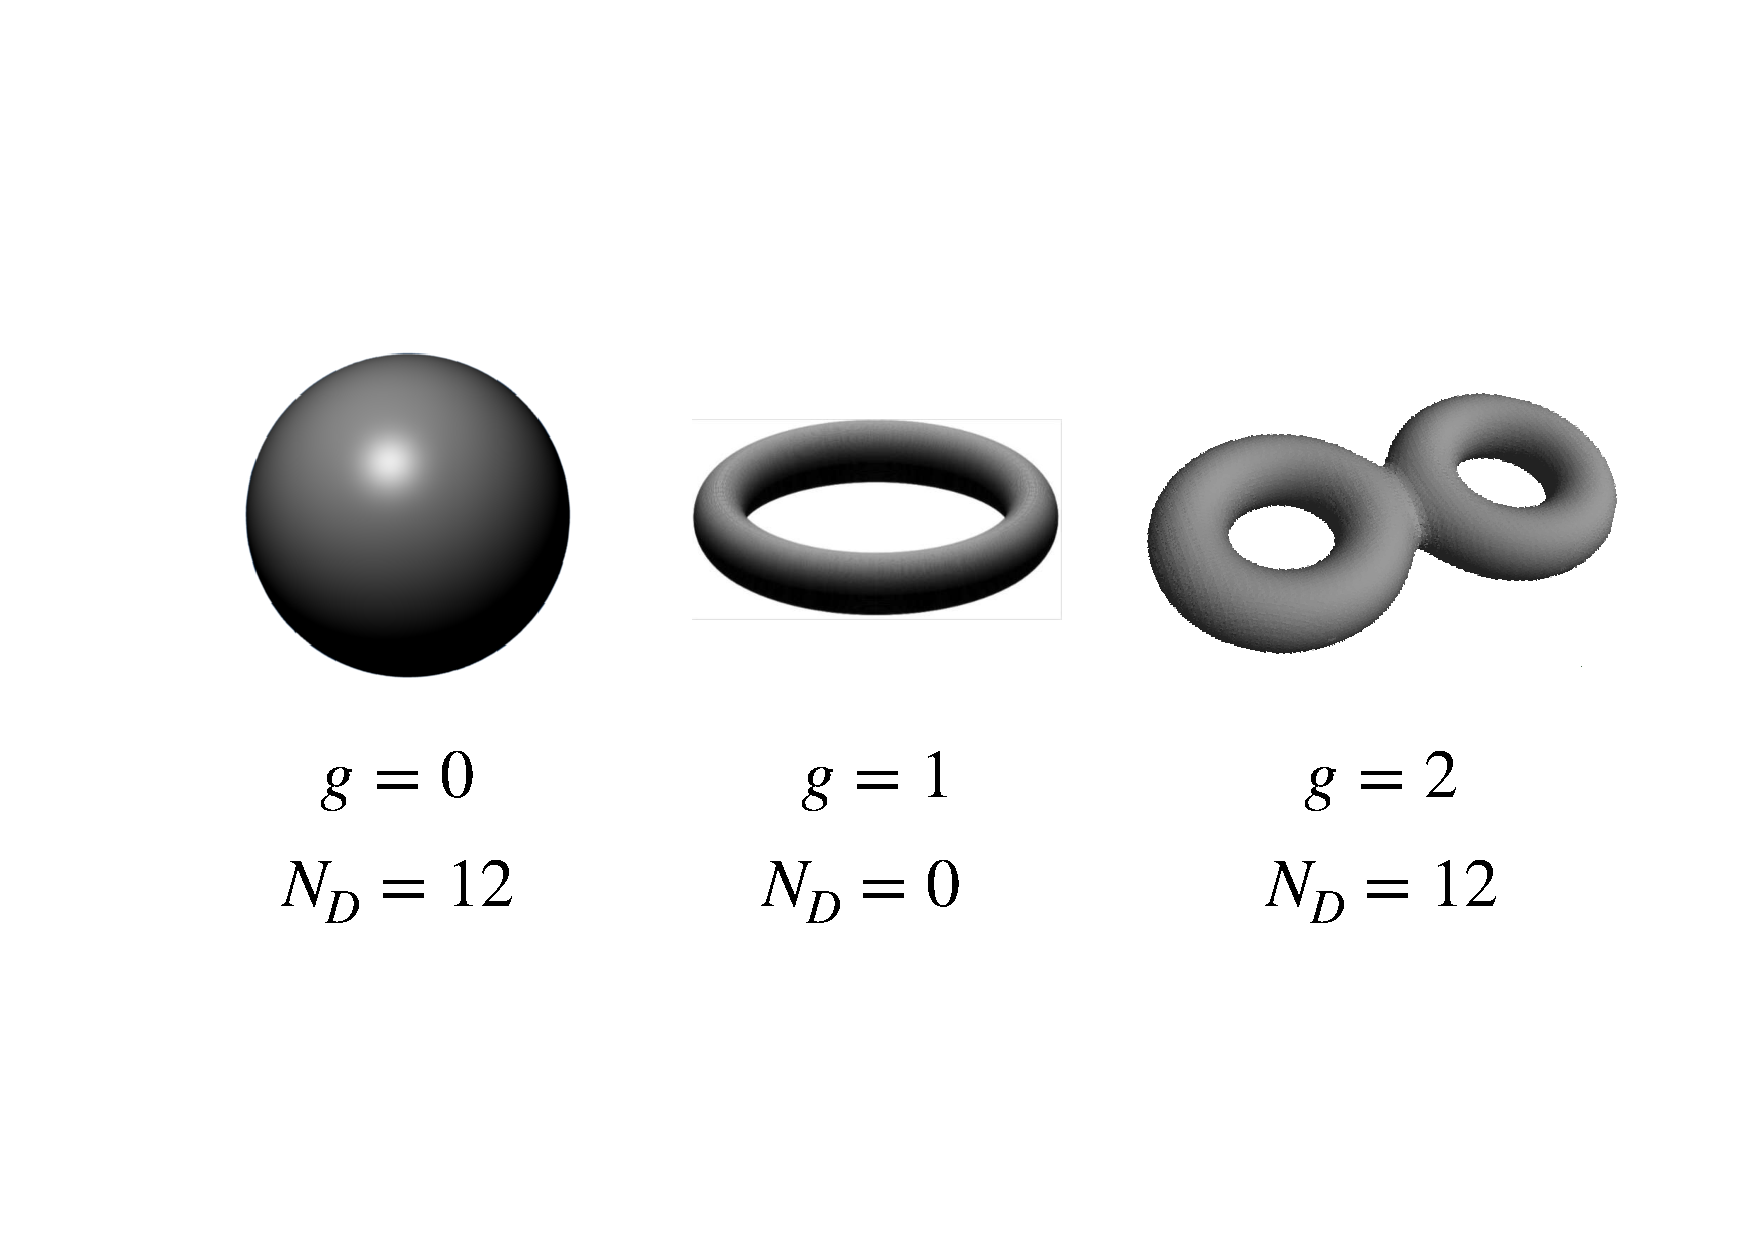
\includegraphics[width=6in]{\MemDiscr/Pics/genus.pages.pdf}
\caption{
۳ مثال از سطوح بسته به همراه جینوس و کمترین تعداد نقاط نقص لازم  برای ساخت آن با مش مثلثی.
}
\label{fig:genus}
\end{center}
\end{figure}


معادلات
\ref{eq:stretchdiscenergy}
و
\ref{eq:bendingdiscenergy}
تغییر انرژی کششی و خمشی یک مش منظم پس از اضافه شدن نقص به مرکز شبکه را توصیف می‌کنند. رقابت میان این دو جمله تعیین می‌کند که یک مش مثلثی کروی به لحاظ انرژی چه شکلی را به خود می‌گیرد. با مقایسه‌ی این دو جمله می‌توان عدد بی بعد  فاپل فون کارمان
\LTRfootnote{Foppl–von Kármán number}
را ساخت
\cite{nelsonPRE2003}
:
\begin{equation}
\gamma = \frac{Y_{2D}R^2}{\kappa}
\label{eq:gamma}
\end{equation}
اگر تمام اضلاع یک مش مثلثی کروی از یک جنس باشند (مدول یانگ و طول اولیه یکسان) در این صورت، عدد فاپل فون کارمان شکل نهایی مش را تایین می‌کند. برای مقادیر زیاد، هزینه‌ی کشش فنر‌ها نسبت به خم شدن بیشتر است و حالت کمینه‌ی انرژی آزاد مجموعه زمانی‌ است که طول تمام اضلاع به طول اولیه‌ خود (انرژی کششی کم) بسیار نزدیک است. از آنجایی که سطح دو بعدی است و قید بسته بودن دارد، به ناچار خمش در محل‌های مشخصی ایجاد می‌شود. از آنجایی که تعداد همسایه‌های مثلث‌های نقاط نقص (۵) کمتر از همسایه‌های مثلث‌های جاهای دیگر (۶) است، هزینه‌ی خم شدن در این نقاط کمتر از جاهای دیگر است و کره شکل بیست‌وجهی
\LTRfootnote{icosehedron}
به خود می‌گیرد.
به همین ترتیب در حد اعداد فاپل فون کارمان کوچک هزینه‌ی کشش در سیستم کم است و سیستم شکل کروی (کمترین خمش) به خود می‌گیرد. در شکل
\ref{fig:gamma}
هندسه‌ی مش مثلثی بسته با ۱۲ نقطه‌ی نقص با گاماهای مختلف نشان داده شده است. در گاماها‌ی کوچک (۴۵) هندسه کروی‌است. این هندسه تا مقدار ۱۵۴ (که مقدار حدی تغییر شکل مش است
\cite{nelsonPRE2003}
) حفظ می‌شود. برای مقادیر گامای بیشتر از ۱۵۴ شکل کره دیگر شکل کمینه‌ی سیستم نخواهد بود و هندسه به طور پیوسته با افزایش گاما به شکل ۲۰ وجهی تغییر می‌کند.
\begin{figure}[h]
\begin{center}
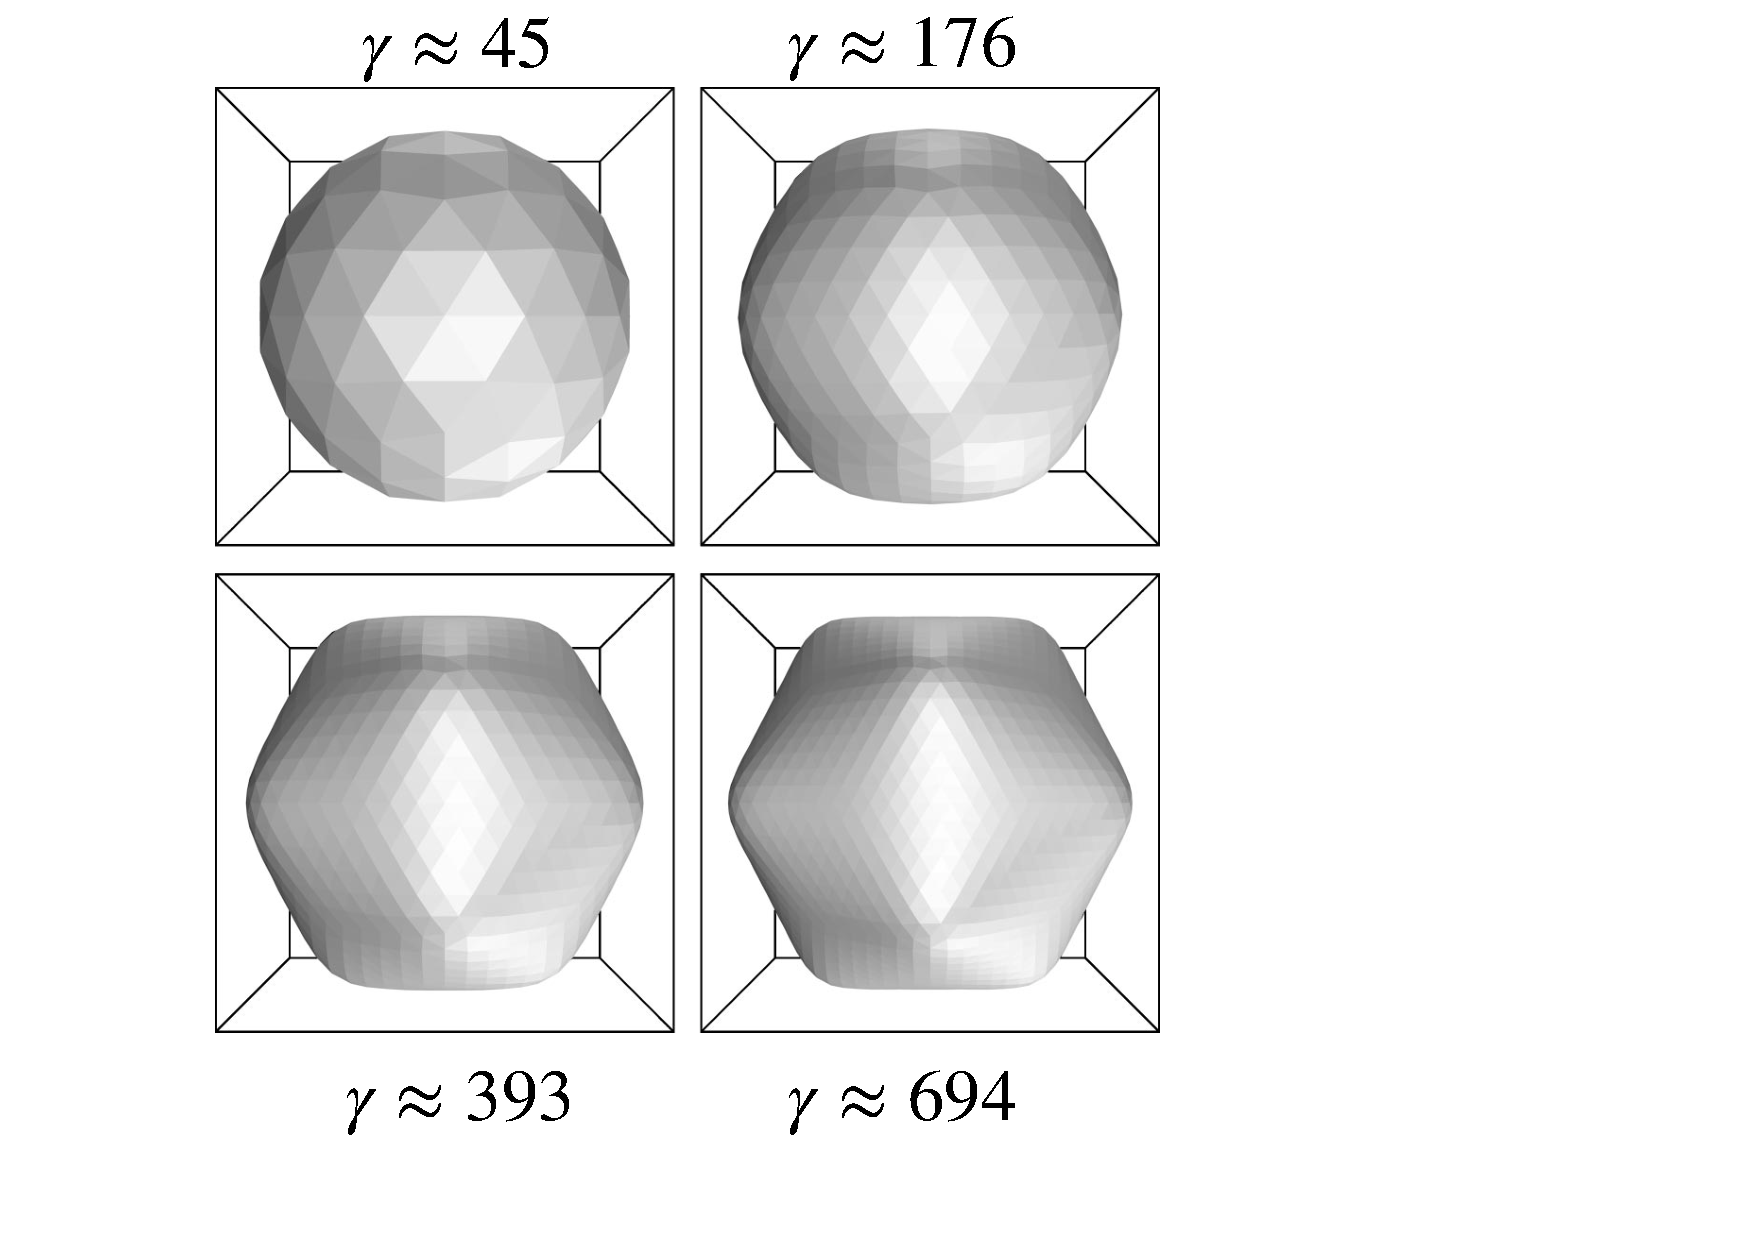
\includegraphics[width=4in]{\MemDiscr/Pics/gamma.pages.pdf}
\caption{
مثال‌هایی از شکل کمینه انرژی مش مثلثی کروی درجه‌ی ۶ با ۱۲ نقطه‌ی نقص. گاما عدد فاپل فون کارمان است. برای مقادیر کم گاما شکل بهینه، کره است و برای مقادیر بالاتر مقدار حدی ۱۵۴، شکل بهینه بیست وجهی است.
}
\label{fig:gamma}
\end{center}
\end{figure}
لازم است تاکید شود که گاما به غیر از مدول‌های الاستیک به اندازه‌ی سطح نیز وا بسته است. در نتیجه در صورتی که مش مثلثی با مدول الاستیک مشخصی ساخته شود، با تنظیم اندازه‌ی مش (یا طول اضلاع) شکل بهینه‌ی سیستم را می‌توان تغییر داد.









\section{
الگوریتم مثلث‌بندی دینامیک
}
\begin{figure}[h]
\begin{center}
\includegraphics[width=\columnwidth]{\MemMethod/Pics/dynamicTri}
\caption{
تغییر مثلث بندی مِش با تغییر موضعی جفت مثلث‌ها میان چهار نقطه. در حالت اولیه (سمت چپ) دو مثلث با رئوس
$ABC$
و
$DBC$
تعریف شده‌است. با تغییر ضلع مشترک بین دو مثلث از 
$BC$
به
$AD$
مثلث بندی جدید با رئوس
$BAD$
و 
$CAD$
تشکیل خواهد شد (سمت راست).
}
\label{fig:dynamicTri}
\end{center}
\end{figure}



روش  مثلث بندی دینامیک\LTRfootnote{dynamic triangulation}
ابتدا توسط دیوید بول\LTRfootnote{David Boal}
و همکارش 
\cite{Boal1992PRA}
در سال ۱۹۹۲برای مِش‌های مثلثی طراحی شد. هدف اصلی این روش، شبیه‌سازی رفتار سیال گون غشا با استفاده از شبکه‌های مثلثی بود. کمی‌ بعد در همان سال، گامپر و کرول با  شبیه‌سازی موفق غشاهای سیال گون، سبب محبوبیت این روش شدند 
\cite{Gompper1992Science}.
این روش را بسیار محبوب کرد. گامپر و کرول در این مطالعه از روش انحنای دو سطحی برای محاسبه‌ی انرژی انحنا استفاده کردند. همانطور که در بخش
\ref{sec:curvatureDiscDef}
توضیح داده شد، این روش برای محاسبه‌ی انحنای غلط است. در سال ۱۹۹۶ گامپر و کرول روش محاسبه‌ی ایتزیکسون را با روش مثلث بندی دینامیکی ترکیب کردند و با موفقیت رفتار سیال‌گون غشا را شبیه‌سازی کردند
\cite{gompper1996}.

در روش مثلث بندی دینامیک دو مثلث مجاور در نظر گرفته می‌شود. رئوس این دو مثلث مانند شکل 
\ref{fig:dynamicTri}
سمت چپ، چهار وجهی 
$ABCD$
را تشکیل خواهد داد. مثلث بندی در ابتدا دو مثلث 
$ABC$
و
$DBC$
را تعریف می‌کند. با حذف ضلع
$BC$
و ایجاد ضلع
$AD$
مثلث بندی جدید با مثلث‌های
$CAD$
و
$BAD$
تشکیل خواهد شد (شکل
\ref{fig:dynamicTri}
سمت راست). تغییر مثلث بندی، انرژی انحنا و کششی مِش را تغییر خواهد داد. همانطور که در شکل با رنگ‌های قرمز و سبز نمایش داده شده، همسایه‌های مثلث‌های آبی در این فرآیند تغییر خواهد کرد. در نتیجه علاوه بر تغییر زاویه‌ی میان مثلث‌های آبی در دو مثلث بندی، زاویه میان همسایه‌ها نیز تغییر خواهد کرد. به لحاظ انرژی کششی، در صورتی که طول ضلع 
$BC$
و
$AD$
متفاوت باشد، انرژی کششی نیز تغییر خواهد کرد. انتخاب مثلث بندی با یک وزن متروپلیس\LTRfootnote{Metropolis}
 انجام می‌شود. در این روش، ابتدا انرژی مثلث بندی در حالت اولیه محاسبه می‌شود
($E_i$),
سپس مثلث بندی تغییر داده می‌شود و انرژی مش در چیدمان جدید محاسبه ‌می‌شود
($E_f$).
 در صورتی که انرژی با مثلث بندی جدید کاهش پیدا کند مثلث بندی جدید حتما پذیرفته می‌شود. در صورتی که انرژی مثلث بندی جدید بیشتر باشد این چیدمان با یک وزن بولتزمن\LTRfootnote{Boltzman}
انتخاب یا رَد خواهد شد. 

به علت ماهیت این الگوریتم بهترین روش برای شبیه‌سازی آن استفاده از روش مانتی کارلو\LTRfootnote{Monte Carlo}
است. گامپر و کرول هنگام ترکیب الگوریتم مثلث بندی دینامیک با روش اندازه‌گیری انحنای ایتزیکسون، محدودیت‌های زیادی در انتخاب طول اضلاع قرار داد. نتیجه‌ی این محدودیت‌ها ایجاد توزیع یکنواخت نقاط بر سطح شبکه‌ی مثلثی و کنترل شکل و اندازه مثلث‌ها در جهت پایدار کردن روش ایتزیکسون بود.

\begin{figure}[h]
\begin{center}
\includegraphics[width=13cm]{\MemMethod/Pics/DT.pdf}
\caption{
نمایش یک مربع (a)، یک مستطیل (b)، و دو شکل غیر مرتبط (c) که همگلی از ۳۴۰ مثلث متساوی الاضلاع تشکیل شده‌اند.
}  
\label{fig:meshDT}
\end{center}
\end{figure} 


همچنین با استفاده از الگوریتم مثلث‌بندی دینامیک 
\cite{Boal1992PRA, Gompper1992Science},
می‌توان اتصالات مختلف
 $\cal G$
را نمونه‌گیری کرد. این الگوریتم مهم‌ترین و پر کاربرد‌ترین روش برای بازسازی مش است که برای شبیه‌سازی اشکال غشا‌ها استفاده می‌شود. با تعمیم این روش
\cite{Kohyama2003PRE},
می‌توان رفتارهای پیچیده‌ی سطوح مایع‌گون (شکل 
\ref{fig:meshDT}c)
 را نیز شبیه‌سازی کرد. با وجود آزادی زیادی که این روش برای مدل سازی غشا‌ها در اختیار ما قرار می‌دهد، این روش محدودیت‌هایی نیز دارد. قدرت اصلی این الگوریتم در تغییر اتصالات مش‌های سخت است. یعنی برای یک تغییر شکل ساده مربعی به مستطیلی (شکل 
\ref{fig:meshDT})
 باید چیدمان نقاط (و اتصالات میانشان) را با دینامیک موضعیِ پخشی تغییر داد. این کار بسیار زمانبر است.






















\clearpage
\clearpage
\chapter{
\centering{
Dynamic Area Redistribution
}
}
\setRL
\clearpage
\def \MemMethod {\Mempath /MembraneMethod}

\section{
چکیده
}
در بخش
\ref{sec:cellmembrane}
مروری کوتاهی بر تارخچه‌ی تحقیقات انجام شده در جهت کشف و بررسی ساختار غشای سلول‌های زنده در قرن‌های ۱۹ و ۲۰ میلادی شده‌است. در بخش
\ref{sec:nuclearenvelope}
ساختار بسته‌ی هسته به صورت مختصر توضیح داده شده‌است.

\section{
مقدمه
}
در روش شبیه‌سازی توزیع دینامیک مساحت
\LTRfootnote{Dynamic Area Redistribution}
اندازه و شکل قسمت‌های مِش به طور پیوسته در حال تغییر است. در این مدل تنش بُرشی هزینه‌ی انرژی نداشته و چگالی دولایه‌ی لیپیدی غشا در سراسر مش ثابت فرض شده. در این رساله از شبکه‌ی مثلثی برای پیاده سازی 
Dynamic Area Redistribution (DAR)
استفاده شده‌است. جهت شبیه‌سازی موفق غشا لازم است انرژی مساحت، حجم، و انحنا به درستی در همه نقاط محاسبه شود. صحت معادلات گسسته بر شبکه‌های منظم و تصادفی در مطالعات گذشتگان اثبات شده است (بخش 
\ref{sec:simRevMesh}
). در درجه‌ی اول صحت این معادلات بر شبکه‌های درهم نیز باید اثبات شود. سپس با استفاده از این شبکه‌ها می‌توان رفتار غشا را مطالعه کرد. ابتدا افت و خیز سطح غشای شبیه‌ سازی شده با این روش مطالعه، سپس شکل غشا برای مقادیر مختلف حجم کاهیده بررسی شد. در نهایت در جهت ارائه‌ی کاربرد این مدل، نحوه‌ی تولید گلبول قرمز نمایش داده شده‌است.


\section{
روش توزیع دینامیک مساحت در شبکه‌ی مثلثی
}
روش توزیع دینامیک مساحت 
\LTRfootnote{Dynamic Area Redistribution}
با هدف  شبیه‌سازی خاصیت سیال‌گون غشا در محیط دینامیک ملکولی در گروه ماده چگال نرم دانشکده فیزیک دانشگاه صنعتی شریف طراحی شده‌است.  غشا سیال است و ملکول‌های لیپید در آن رفتار پخشی دارند. در صورتی که به نقطه‌ای از غشا تنش بُرشی توسط نیروی خارجی وارد شود، ملکول‌های لیپیدی بر سطح غشا حرکت می‌کنند. هنگامی که نیروی‌ خارجی متوقف شود، ملکول‌های لیپید دلیلی برای بازگشت به محل اولیه خود ندارند و مانند یک سیال به حرکت پخشی خود ادامه می‌دهند. 

\begin{figure}[h]
\begin{center}
\includegraphics[width=12cm]{\MemMethod/Pics/meshDiffusion.pdf}
\caption{
شبکه بندی سطح غشا تشکیل شده از 
$N$
ملکول لیپیدی را نمایش می‌دهد. در هنگام تعادل ترمودینامیکی چگالی ملکول‌ها در هر تکه از شبکه به طور متوسط
$\rho=N/A_0$
است.
}
\label{fig:cylindermesh}
\end{center}
\end{figure}

غشایی با مساحت 
$A_0$
را فرض می‌کنیم که از 
$N$
ملکلول لیپیدی تشکیل شده‌است. در صورتی که سطح غشا با 
$M$
قسمت با مساحت 
$A_0/M$
شبکه بندی شود، هنگام  تعادل ترمودینامیکی، به طور متوسط چگالی ملکول‌های لیپیدی در هر قسمت از شبکه برابر با 
$\rho=N/A_0$
است. اگر تنش  به قسمت
$i$
از شبکه وارد شود که باعث انبساط آن تکه شود، چگالی ملکول‌های آن کمی کمتر از متوسط خواهد شد،
$\rho_i=\rho^-$
. از آنجایی که تعداد ملکلو‌ل‌ها در سطح غشا یکسان است و غشای لیپیدی ضریب فشردگی بسیار بزرگی دارد، چگالی تمام قسمت‌های دیگر شبکه کمی افزایش می‌یابد (
$\rho_j=\rho^+$
برای هر قسمت که
$i\neq j$
). از آنجایی که غشا در تعادل ترمودینامیکی به سر می‌برد با گذشت زمان کم ملکلول‌های غشا (با دینامیک پخشی) در قسمت‌های مختلف شبکه جابجا شده و چگالی ملکولی در تمام قسمت‌ها را دوباره یکسان می‌کنند. در نتیجه تا زمانی که مساحت کل غشا تغییر نکند اندازه‌ی قسمت‌های مختلف شبکه می‌تواند با دمای محیط اُفت  و خیز کند. در این توصیف هر قسمت از شبکه نماینده‌ی تعداد ثابتی از ملکول‌های لیپیدی نیست ولی چگالی عددی ملکلول‌ها در سراسر غشا یکسان است.

روش توزیع دینامیک مساحت روی هر شبکه‌ بندی قابل پیاده‌سازی است. در این رساله، این روش بر روی شبکه‌های مثلثی پیاده‌سازی شده‌است. در دهه‌های گذشته مطالعات زیادی بر نحوه‌ی شبیه‌سازی با استفاده از شبکه‌های مثلثی شده‌است. در نتیجه نحوه‌ی گسسته سازی انرژی‌های مورد نیاز برای شبیه‌سازی یک غشا (انرژی خمش، مساحت، و حجم) بر بستر این شبکه‌ها از مطالعات گذشتگان در دسترس است. برای شبیه‌سازی رفتار سیال‌گون غشا کافی ‌است که انحنای غشا بر روی سطح به درستی تعریف شود و حجم و مساحت کل غشا رد طول شبیه‌سازی قابل کنترل باشد. 

در آخر لازم است به این نکته اشاره شود که از آنجایی که غشا‌ مدول یانگ ندارد، تغییر شکل‌های کُره-بیست وجهی که حاصل از رقابت انرژی کشسانی و انرژی خمشی است (جزئیات بیشتر در بخش 
\ref{sec:gammaTransition}
) در آن‌ها دیده نخواهد شد.






\section{
تهیه‌ی مِش
}
\begin{figure}[h]
\begin{center}
\includegraphics[width=12cm]{\MemMethod/Pics/MeshTypes.pdf}
\caption{
عکس چهار نوع مِش استفاده شده در این رساله. مِش منظم (بالا سمت چپ)، تصادفی (بالا سمت راست)، دَرهَم منظم (پایین سمت چپ)، و مِش دَرهَم تصادفی (پایین سمت راست).
}
\label{fig:meshTypesMesthod}
\end{center}
\end{figure}
در شکل
\ref{fig:meshTypesMesthod}
نمونه‌ای از مِش‌هایی که در این رساله استفاده شده را می‌توان یافت. مِش‌ها به ترتیب زیر قابل تهیه هستند:
\subsection{
مِش منظم
}
مش منظم با شبکه‌‌بندی کردن یک بیست وجهی منتظم ساخته می‌شود. در این شبکه‌ بندی ۱۲ نقطه‌ی نقص با درجه‌ی ۵ در ۱۲ گوشه‌ی بیست وجهی ایجاد خواهد شد و نقاط دیگر همگی از درجه‌ی ۶ خواهند بود. در نتیجه به ازای هندسه بسیار متقارن کُره تنها یک نمونه از چنین شبکه‌ای به ازای تعداد نقاط وجود دارد. همچنین  برای ساخت چنین مِشی تنها می‌توان  تعداد مشخصی نقطه که با رابطه‌ی 
\begin{equation}
N_{mesh}=10\times i^2+2,
\end{equation}
محاسبه می‌شود، داشت،  که در اینجا 
$i$
مقادیر صحیح غیر صفر دارد. ‌شبکه‌ بندی با هر نرم‌افزار مش بندی قابل انجام است. در این مطالعه ما از نرم افزار 
Blender
برای تولید این مِش به خصوص استفاده کردیم. 

\subsection{
مِش تصادفی
}
مقدمه‌ی تهیه‌ی این نوع مش  قرار دادن 
$N$
نقطه به شکل تصادفی بر سطح یک کُره‌ به شعاع ۱ است. سپس به کمک 
$N$
پتانسیل فنر هارمونیک با ضریب سختی زیاد، این نقاط را به مرکز کُره متصل کرده و بر سطح کُره مقید می‌کنیم. سپس میان این نقاط برهمکنش بلند بُرد دافعه تعریف می‌کنیم. هر برهمکنش دافعه‌ی بلند بُردی که  توزیع تقریبا یکنواخت نقاط بر سطح کُره ایجاد کند مورد قبول است. در این رساله از پتانیسل 
\begin{equation}
U_{EV}=10^{-3}\left(\frac{2\rho_0}{r}\right)^6,
\end{equation}
استفاده شد. در اینجا 
$r$
فاصله‌ی فضایی نقاط از یکدیگر بوده و 
$\rho_0$
شعاع متوسط هر نقطه روی کُره است. شعاع متوسط کُره با شعاع 
$N$
دایره تخمین زده شده‌است که  سطح کُره را پوشش می‌دهند
\begin{equation}
N\pi\rho_0^2=4\pi\rightarrow \rho_0=\frac{2}{\sqrt{N}}.
\end{equation} 
سپس ذرات تحت دینامیک لانژون شروع به حرکت کرده و با انتخاب دمای پایین برای ترموستات لانژون می‌توان سرعت ذرات را پله پله کم کرد تا جایی که ذرات در فاصله‌ی تعادلی نسبت به یکدیگر قرار گیرند. البته از هر روش کمینه کردن انرژی\LTRfootnote{energy minimisation}
برای یافتن مختصات تعادلی نقاط می‌توان استفاده کرد. پس از یافت مختصات تعادلی نقاط با استفاده از الگوریتم مثلث‌ بندی دِلونی\LTRfootnote{Delaunay triangulation algorithm}
\cite{DelaunayTriangulation1997}
یک شبکه‌ی مثلثی تصادفی ایجاد خواهد شد. با تکرار این دستورنامه با استفاده از بذر‌های\LTRfootnote{seed}
 مختلف برای تولید اعداد تصادفی غیر یکسان می‌توان مِش‌های تصادفی متفاوتی تولید کرد.

\subsection{
مِش‌های درهم
}
برای تغییر توزیع مساحت مثلث‌های مِش‌های منظم و تصادفی‌  نقاط آن را با فنر‌های هارمونیک با ضریب سختی بالا مقید به حرکت بر سطح کُره کرده و سپس به تمام نقاط، سرعت و جهت تصادفی اختصاص داده می‌شود. با محدود کردن طول ارتفاع مثلث‌های مش با پتانسیل 
$U_{h}$
(جزئیات این پتانسیل در بخش 
\ref{sec:auxPotentials}
قرار دارد) حد پایین برای اندازه‌ی مثلث‌ها تعیین شد. این پتانسیل تضمین می‌کند که اضلاع مثلث‌ها بر اثر حرکت کاتوره‌ای نقاط همدیگر را قطع نکنند. ولی این پتانسیل برای جلوگیری از تا شدن مثلث‌ها بر روی سطح کافی نیست. برای پیشگیری از این اتفاق، پتانسیل غیر خطی خمشی دوسطحی
$U_{\phi}$
(جزئیات این پتانسیل در بخش 
\ref{sec:auxPotentials}
قرار دارد) میان تمام جفت مثلث‌های مش تعریف شد. در نتیجه دینامیک چنین نقاطی تحت معادله‌ی حرکت نیوتن (انتگرال گیری وِرلِه سرعتی\LTRfootnote{velocity Verlet})
 مساحت‌ مثلث‌ها افت و خیز می‌کند و توپولوژی اولیه مِش استفاده شده کاملا محفوظ می‌ماند.
 






\section{
پتانسیل کنترل مساحت و حجم
}
\begin{figure}[tbp]
\begin{center}
\includegraphics[width=14cm]{\MemRes/Pics/UnitSphereAreaVolume}
\caption{
مساحت (ستون چپ) و حجم (ستون راست) محاسبه‌ شده برای چهار نوع مش‌های کُروی بر اساس تعداد نقاط روی مش رسم شده‌است. مساحت کل، به دو روش، با جمع مساحت‌های ورنوی (نقاط بنفش) و جمع مساحت‌های بریسنتریک (نقاط خاکستری) محاسبه شده‌است. دقت در اندازه‌گیری مساحت و حجم (نقاط آبی) برای تمام مش‌ها با افزایش تعداد نقاط روی مش، افزایش می‌یابد. تصویر مش نمونه از هر نوع مش استفاده شده در محاسبات کنار هر ردیف رسم شده‌است. به غیر از مش منظم (که تنها یک نمونه از آن برای هر تعداد نقطه وجود دارد) مقادیر محاسبه شده حاصل از میان‌گین گیری بر روی ۵۰ نمونه‌ی مستقل انجام شده‌است.
}
\label{fig:unitsphereAreaVolume}
\end{center}
\end{figure}

جهت بررسی دقت اندازه‌گیری مساحت و حجم برای مش‌های مختلف، مش‌های کروی با تعداد نقاط مختلف انتخاب شد.  مساحت مش‌ها به دو روش محاسبه شد، با جمع  مساحت‌ وُرُنُی رئوس (نقاط بنفش) و جمع مساحت بریسنتریک (نقاط خاکستری). جهت بررسی میزان دقت در اندازه‌گیری،  نتیجه‌ی محاسبات بر مساحت کُره (
$4\pi r_0^2$
)  تقسیم شده‌است. نتایج محاسبات در شکل
\ref{fig:unitsphereAreaVolume}
رسم شده‌است. همانطور که می‌بینید دقت اندازه‌گیری برای تمامی مش‌ها با افزایش تعداد نقاط بهتر می‌شود. لازم به ذکر است  از آنجایی که تمام نقاط مش‌ها روی سطح پوسته‌ی کُروی قرار دارد، یا به عبارت دیگر مش بر داخل یک کره‌ مماس است، مساحت و حجم آن همیشه از کره کمتر خواهد بود.




مشابه به مساحت، حجم نیز برای تمامی مش‌ها با دقت بسیار خوبی قابل اندازه‌گیری‌است. در نتیجه مش‌های درهم برای اندازه‌گیری مساحت و حجم کره مناسب هستند. از آنجایی که غشا‌ها اشکال پیچیده‌تری نسبت به کره دارند، صحت محاسبات برای اشکالی به غیر از کره نیز باید بررسی شود. با اضافه کردن جمله‌ی هارمونیک کروی به مکان شعاعی تمام نقاط مش، می‌توان شکل مش را تغییر داد،
\begin{eqnarray}
r(\theta,\phi)=r_0+r_0|u_{\ell,m}|Y_{\ell,m}(\theta,\phi).
\label{eq:rDeformed}
\end{eqnarray}
با انتخاب
$\ell=2$
و
$m=0$
برای هماهنگ‌ کروی، می‌توان مش‌های دمبلی شکل  تولید کرد. میزان تغییر شکل به شدت مُد
$u_{2,0}$
بستگی دارد. هزینه‌ی انرژی تغییر مساحت یک کره به یک شکل دمبلی طبق معادله‌ی
\ref{eq:AreaGLFluctuationAmplitude}
قابل محاسبه ‌است،
\begin{equation}
E_A=\frac{2}{\pi}|u_{2,0}|^4,
\label{eq:AreaEnergyULM20}
\end{equation}
در معادله‌ی فوق 
$k_A=1[\varepsilon/l^2]$
و
$r_0=1[l]$
فرض شده‌است. نیروی بازگرداننده که با این تغییر شکل مقاومت می‌کند با مشتق گیری از انرژی در فضای مُد قابل محاسبه‌ می‌باشد، 
\begin{equation}
-\frac{\partial E_A}{\partial u_{2,0}}=-\frac{8}{\pi}|u_{2,0}|^3,
\label{eq:AreaForceULM20}
\end{equation}


به همین ترتیب با جایگذاری 
$k_V=1[\varepsilon/l^3]$
در معادله‌ی
\ref{eq:VolumeGLFluctuationAmplitude}
می‌توان انرژی تغییر حجم مش زمانی که از  شکل کره به شکل دمبلی تغییر می‌کند را بر حسب شدت مُد محاسبه کرد،
\begin{equation}
E_V= \frac{3}{8\pi}|u_{2,0}|^4.
\label{eq:VolumeEnergyULM20}
\end{equation}

با مشتق ‌گیری نسبت به شدت مُد، مقدار نیرویی که با تغییر شکل مش مقاومت می‌کند را می‌توان بر حسب شدت مد محاسبه کرد،
\begin{equation}
-\frac{\partial E_V}{\partial u_{2,0}}= -\frac{3}{2\pi}|u_{2,0}|^3,
\label{eq:VolumeForceULM20}
\end{equation}

\begin{figure}[tbp]
\begin{center}
\includegraphics[width=14cm]{\MemRes/Pics/UnitSphereDeformation_mesh_10_Areavolume}
\caption{
انرژی مساحت (ستون 
$(a)$
) و حجم (ستون 
$(b)$
) محاسبه‌ شده حاصل از تغییر شکل مش کروی با اضافه شدن مد
$Y_{2,0}(\theta,\phi)$
با شدت‌های مختلف برای چهار نوع مش رسم شده‌است. انرژی مساحت برای دو روش محاسبه‌ی مساحت کل، جمع مساحت‌های ورنوی (نقاط بنفش) و جمع مساحت‌های بریسنتریک (نقاط خاکستری)، و انرژی حجم (نقاط آبی) با جمع روی حجم هرم‌ها محاسبه شده‌است. خطوط مشکی برای ستون‌های 
$(a)$
و
$(b)$
به ترتیب از رسم معادلات
\ref{eq:AreaEnergyULM20}
و
\ref{eq:VolumeEnergyULM20}
حاصل شده‌است. نیروی بازگرداننده برای تغییر مساحت و حجم در ستون‌های 
$(c)$
و
$(d)$
رسم شده.  پیش‌بینی‌ مرتبه‌ی دوم نیروی بازگرداننده برای تغییر مساحت وحجم با توجه به معادلات
\ref{eq:AreaForceULM20}
و
\ref{eq:VolumeForceULM20}
با خط مشکی رسم شده است. شدت مد 
$u_{2,0}=0$
مربوط به شکل کاملا کروی (عکس سمت چپ) و شدت مد 
$u_{2,0}=1$
مربوط به شکل دمبلی (عکس سمت راست) است. یک نمونه از هر مش برای حالت کروی و دمبلی در ردیف مربوته رسم شده‌است. به غیر از مش منظم (که تنها یک نمونه از آن برای هر تعداد نقطه وجود دارد) مقادیر محاسبه شده حاصل از میان‌گین گیری بر روی ۵۰ نمونه‌ی مستقل انجام شده‌است.
}
\label{fig:unitsphereAreaVolumeULM20}
\end{center}
\end{figure}


در شکل
\ref{fig:unitsphereAreaVolumeULM20}
نتیجه‌ی محاسبات عددی در کنار پیش‌بینی نظری برای انرژی و نیروی حاصل از تغییر شکل رسم شده است. شدت مد
$u_{2,0}=0$
مربوط به مش کاملا کروی است (عکس‌های سمت چپ) و شدت مد 
$u_{2,0}=1$
مربوط به مش‌های دمبلی شکل است (عکس‌های سمت راست). هر ردیف محاسبات را برای یک نوع مش نشان می‌دهد که با  عکسی از آن مش مشخص شده‌است. به ترتیب در ستون‌های 
$(a)$
،
$(b)$
،
$(c)$
، و
$(d)$
تغییر انرژی مساحت، انرژی حجم، نیروی مساحت، و نیروی حجم به صورت نقاط بنفش (ورنوی) و خاکستری (بریسنتریک) برای مساحت و نقاط آبی برای حجم به همراه پیش‌بینی استخراج شده از محاسبات افت و خیز (خط مشکی) رسم شده‌است. 

داده‌های شکل 
\ref{fig:unitsphereAreaVolumeULM20}
نشان می‌دهد که رفتار انرژی و نیرو برای تغییر شکل‌های کوچک با پیش‌بینی مستخرج از محاسبات افت و خیز همخوانی دارد. از آنجایی که محاسبات افت و خیز برای شدت مد‌های کوچک و تا مرتبه‌ی دوم در 
$u_{\ell,m}$
درنظر گرفته شده‌است برای شدت‌ مد‌های بزرگ فاقد اعتبار است. ولی رفتار کلی محاسبات عددی و معادلات
\ref{eq:AreaEnergyULM20}
،
\ref{eq:VolumeEnergyULM20}
،
\ref{eq:AreaForceULM20}
، و
\ref{eq:VolumeForceULM20}
برای شد‌ت مد 
$|u_{\ell,m}|>0.5$
نیز همخوانی دارد. می‌توان نتیجه گرفت که محاسبات لازم برای اندازگیری مساحت و حجم غشا برای شکل‌های کروی و همچنین شکل‌های غیر کروی حاوی انحنای زین اسبی بر روی مش‌های معمولی  و  درهم به خوبی قابل پیاده‌سازی است.












\section{
پتانسیل انحنای متوسط
}
یک مِش ممکن است از نقاط با درجه‌های مختلفی تشکیل شده باشد. مثلا مش منظم از نقاط با درجات ۵ و ۶ ساخته شده و مش‌های تصادفی قالبا درجات ۵، ۶، و ۷ دارند. پتانسیل انحنا بر روی لیس رئوسی تعریف می‌شود که درجه‌ی یکسان دارند. در نتیجه به ازای هر درجه‌ی موجود در مش  لیست مجزایی از رئوس با آن درجه تشکیل داده می‌شود. سپس پتانسیل انحنا برای هر لیست درجه به طور مجزا تعریف می‌شود. نحوه‌ی محاسبه‌ی انحنا میان این پتانسیل‌ها یکسان بوده و تنها تعداد جملاتی که بر روی آن جمع زده می‌شود متفاوت است. در نتیجه برای هر لیست از رئوس درجه‌ی 
$n$
یک پتانسیل 
$n+1$
ذره‌ای نیاز است.


پتانیسیل  انحنا برای مدل یولیشر به شکل زیر پیاده‌سازی شده،
\begin{equation}
U_b^J=\frac{3}{4}\kappa\sum_i\frac{\left[\sum_{j(i)}\ell_{ij}\phi_{ij}\right]^2}{\sum_{j,j'(i)}\ell_{ij}\ell_{ij'}\sin(\theta_{jij'})}
\label{eq:UbJDiscrete}
\end{equation}
در اینجا تعریف پارامتر‌های 
$\ell_{ij}$
و
$\phi_{ij}$
مطابق شکل 
\ref{fig:trianglePairAngle}
است. در صورت معادله‌ی فوق جمع روی تمام رئوس همسایه نقطه‌ی 
$i$
است و در مخرج جمع روی تمام مثلث‌هایی است که نقطه‌ی 
$i$
میان رئوس آن‌هاست. باید توجه ویژه با انتخاب جهت زاویه‌ی دوسطحی کرد. زاویه‌ی دوسطح میان ۴ نقطه تعریف می‌شود و ترتیب دو نقطه‌ی میانی علامت زاویه‌ی دوسطحی را تغییر می‌دهد. برای کُره لیست نقاط دوسطحی باید طوری تنظیم شود که تمام زوایای دوسطحی روی کُره مثبت باشد.

به شکل مشابه می‌توان پتانسیل انحنا را برای مدل گامپر، گامپر-برسنتریک، و یولیشر-ورنوی تعریف کرد،
\begin{equation}
U_b^\text{GK}=\kappa\sum_i\frac{\left[\sum_{j(i)}(\cot\theta_1^{ij}+\cot\theta_2^{ij})(\vec r_i-\vec r_j)\right]^2}{\sum_{j(i)}\ell_{ij}^2(\cot\theta_1^{ij}+\cot\theta_2^{ij})},
\label{eq:UbGKDiscrete}
\end{equation}

\begin{equation}
U_b^{GKB}=\frac{3}{4}\kappa\sum_i\frac{\left[\sum_{j(i)}(\cot\theta_1^{ij}+\cot\theta_2^{ij})(\vec r_i-\vec r_j)\right]^2}{\sum_{j,j'(i)}\ell_{ij}\ell_{ij'}\sin(\theta_{jij'})},
\end{equation}

\begin{equation}
U_b^{JV}=\kappa\sum_i\frac{\left[\sum_{j(i)}\ell_{ij}\phi_{ij}\right]^2}{\sum_{j(i)}\ell_{ij}^2(\cot\theta_1^{ij}+\cot\theta_2^{ij})}.
\end{equation}

در معادلات فوق فرض شده که سطح انحنای ذاتی ندارد. با استفاده از معادله‌ی 
\ref{eq:bendingDiscretisationSpontaneous}
می‌توان معادلات فوق را برای حالتی که خمش ذاتی 
$C_0$
وجود داشته باشد، بازنویسی کرد. برای یولیشر معادلات به شکل

\begin{equation}
\begin{aligned}
U_b^J=\frac{1}{2}\kappa\sum_i&\frac{3}{2}\frac{\left[\sum_{j(i)}\ell_{ij}\phi_{ij}\right]^2}{\sum_{j,j'(i)}\ell_{ij}\ell_{ij'}\sin(\theta_{jij'})}\\
&-C_0\sum_{j(i)}\ell_{ij}\phi_{ij}\\
&+\frac{1}{6}C_0^2\sum_{j,j'(i)}\ell_{ij}\ell_{ij'}\sin(\theta_{jij'}),
\end{aligned}
\end{equation}
برای گامپر،
\begin{equation}
\begin{aligned}
U_b^\text{GK}=\frac{1}{2}\kappa\sum_i&2\frac{\left[\sum_{j(i)}(\cot\theta_1^{ij}+\cot\theta_2^{ij})(\vec r_i-\vec r_j)\right]^2}{\sum_{j(i)}\ell_{ij}^2(\cot\theta_1^{ij}+\cot\theta_2^{ij})}\\
&-C_0\sqrt{\left[\sum_{j(i)}(\cot\theta_1^{ij}+\cot\theta_2^{ij})(\vec r_i-\vec r_j)\right]^2}\\
&+\frac{1}{8}C_0^2\sum_{j(i)}\ell_{ij}^2(\cot\theta_1^{ij}+\cot\theta_2^{ij}),
\end{aligned}
\end{equation}
برای گامپر-بریسنتریک،
\begin{equation}
\begin{aligned}
U_b^{GKB}=\frac{1}{2}\kappa\sum_i&\frac{3}{2}\frac{\left[\sum_{j(i)}(\cot\theta_1^{ij}+\cot\theta_2^{ij})(\vec r_i-\vec r_j)\right]^2}{\sum_{j,j'(i)}\ell_{ij}\ell_{ij'}\sin(\theta_{jij'})}\\
&-C_0\sqrt{\left[\sum_{j(i)}(\cot\theta_1^{ij}+\cot\theta_2^{ij})(\vec r_i-\vec r_j)\right]^2}\\
&+\frac{1}{6}C_0^2\sum_{j,j'(i)}\ell_{ij}\ell_{ij'}\sin(\theta_{jij'}),
\end{aligned}
\end{equation}
و در نهایت برای یولیشر-ورنوی به شکل
\begin{equation}
\begin{aligned}
U_b^{JV}=\frac{1}{2}\kappa\sum_i&2\frac{\left[\sum_{j(i)}\ell_{ij}\phi_{ij}\right]^2}{\sum_{j(i)}\ell_{ij}^2(\cot\theta_1^{ij}+\cot\theta_2^{ij})}\\
&-C_0\sum_{j(i)}\ell_{ij}\phi_{ij}\\
&+\frac{1}{8}C_0^2\sum_{j(i)}\ell_{ij}^2(\cot\theta_1^{ij}+\cot\theta_2^{ij}),
\end{aligned}
\end{equation}

قابل محاسبه‌ است.





\section{
پتانسیل‌های تکمیلی
\label{sec:auxPotentials}
}


\section{
موتور محاسباتی
OpenMM
}

\section{
آماده سازی شبیه‌سازی
}

\section{
نرم افزار مدل مجازی سلول
}





\clearpage
\clearpage
\chapter{
\centering{
نتایج
}
}
%\setRL
\clearpage
\def \MemModel {\Mempath /MembraneModel}

\section{
چکیده
}
در بخش
\ref{sec:cellmembrane}
مروری کوتاهی بر تارخچه‌ی تحقیقات انجام شده در جهت کشف و بررسی ساختار غشای سلول‌های زنده در قرن‌های ۱۹ و ۲۰ میلادی شده‌است. در بخش
\ref{sec:nuclearenvelope}
ساختار بسته‌ی هسته به صورت مختصر توضیح داده شده‌است.

\section{
مقدمه
}
برای مدل‌سازی غشاها ابتدا پوسته‌های نازک را بررسی خواهیم کرد. توصیف پوسته‌های نازک را با بررسی انرژی خمشی و انرژی کششی یک محیط پیوسته آغاز خواهیم کرد. پس حل معادلات پیوسته، این معادلات را برای مجموعه نقاط در فضا که بر روی شبکه‌ی مثلثی قرار دارند حل می‌کنیم. سپس تغییرات انرژی در صورت ایجاد نقاط نقص بر روی شبکه را محاسبه خواهیم کرد. 


مقاله الکساندرا مرجع ۷ در مقده تيوری خیلی خوب راجع به آنالیز فرکانس نوشته


\begin{figure}[h]
\begin{center}
\includegraphics[width=4in]{\Mempath/Pics/Membrane_fluctuations}
\caption{
مجموعه تصاویر پست سر هم از تغییر شکل یک غشای لیپیدی را با تصویر برداری فلورسانت در بازه‌های ۵ ثانیه‌ای نشان می‌دهد. خط مقیاس سفید رنگ اندازه‌ی ۵ میکرومتر را نشان می‌دهد. 
\cite{ParthasarathyMembraneMeasurement}
}
\label{fig:flucmem}
\end{center}
\end{figure}

شگل 
\ref{fig:flucmem}
تغییر شکل یک غشای لیپیدی غول آسا (قطر حدود ۱۰ میکرون) در بازه‌های زمانی ۵ ثانیه نشان می‌دهد
\cite{ParthasarathyMembraneMeasurement}
. از نظر انرژی تغییر شکل این غشا را می‌توان به دو بخش کلی تقسیم کرد. تغییر انرژی ناشی از خم شدن و تغییر حاصل از کشش سطح غشا. شکل
\ref{fig:elasticdeformation}
الف، تغییر شکل یک عنصر سطحی بر اثر خمش را نشان می‌دهد. خمش سطح را می‌توان با اندازه‌ی شعاع دو دایره که بر عنصر سطح مماس هست، توصیف کرد. همچنین شکل 
\ref{fig:elasticdeformation}
ب، تغییر شکل عنصر سطح به علت ایجاد کشش در سطح نشان می‌دهد. تغییر سطح با اختلاف مساحت عنصر سطح با حالت کشیده نشده توصیف می‌شود.
\begin{figure}[h]
\begin{center}
\includegraphics[width=4in]{\Mempath/Pics/surface elemnts.pages.pdf}
\caption{
تغییر شکل عنصر سطحی بر اثر الف، خمش و ب، کشش.
}
\label{fig:elasticdeformation}
\end{center}
\end{figure}


\section{
انرژی آزاد غشا
}
\setRL
%\pagenumbering{arabic} 


\subsection{
انرژی کشش در سطح
}
اگر فرض کنیم جابجایی روی یک عنصر سطحی حاصل از کشیده‌ یا فشرده شدن سطح با بردار 
$u$
توصیف شود، با فرض خطی بودن عکس العمل ماده، انرژی پتانسیل حاصل از تغییر شکل سطح را می‌توان با معادله‌ی زیر بررسی کنیم.

\begin{equation}
E_{stretching}=\frac{1}{2}Y_{2D}A\varepsilon^2
\end{equation}
که اینجا 
$Y_2D$
مدول دو بعدی یانگ،
$A$
سطح عنصر در حالت کشیده نشده، و
$\varepsilon$
تانسور کرنش است. تانسور کرنش برای سطح دو بعدی به شکل زیر تعریف می‌شود:
\begin{equation}
\varepsilon_{ij} = \frac{1}{2}(u_{ij}+u_{ji})
\end{equation}


.
 
 
 
 
 
 
 
 
 
 
 
 
 
 
 
\setRL
%\pagenumbering{arabic} 


\subsection{
انرژی خمش سطح
}
انرژی خمش یک سطح را می‌توان با انرژي هلفریش
\cite{Helfrich1973}
 کمی کرد،
\begin{equation}
E_{bending}=\int dS\left\{\frac{1}{2}\kappa (H-H_s)^2 +\tilde \kappa K_0\right\}
\label{eq:helfrish}
\end{equation}
در اینجا
\begin{equation}
H = \frac{1}{R_1}+\frac{1}{R_2}
\end{equation}
خمش سطح است که با شعاع دو دایره‌ی مماس بر عنصر سطح بیان می‌شوند (
\ref{fig:elasticdeformation}
). 
$H_s$
خمش زاتی سطح را مشخص می‌کند که همانند خمش،
$H$
تعریف می‌شود. برای مثال خمش زاتی سطحی که در تمام جهت‌ها علاقه دارد شعاع 
$R_s$
داشته باشد، 
\begin{equation}
H_s = \frac{2}{R_s}
\end{equation}
است. 
$K_0$
خمش گاووسی است که به شکل 
\begin{equation}
H_s = \frac{2}{R_s}
\end{equation}
تعریف می‌شود. همچنین 
$\kappa$
و
$\tilde\kappa$
به ترتیب سختی خمشی و سختی خمش گاووسی است. بنا به قضیه گاووس-بونت
\LTRfootnote{Gauss–Bonnet}
انتگرال روی سطح خمش گاووسی پاسخی ساده دارد،
\begin{equation}
\int dS \tilde \kappa K_0=4\pi\tilde\kappa(1-g)
\end{equation}
که در معادله‌ی بالا 
$g$
جینوس 
\LTRfootnote{genus}
سطح، یا تعداد سوراخ یا تعداد دسته‌
\LTRfootnote{handle}
است. اگر پوسته‌ی مورد نظر در طول مطالعه تغییر توپولوژی ندهد حاصل این انتگرال همیشه ‌یک عدد ثابت خواهد بود. در صورتی علاقه‌ی ما محاسبه‌ی نیرو‌های خمشی (مشتق جمله انرژي) یا اختلاف انرژی خمشی باشد، جمله‌ی ثابت خمش گاووسی در محاسبات اهمیت نخواهد داشت.
\subsubsection{
محاسبه‌ی انرژی خمش کره
}
برای مثال انرژی خمش یک کره به شعاع 
$R$
را با رابطه‌ی هلفریش محاسبه می‌کنیم. معادله‌ی 
\ref{eq:helfrish}
به شکل زیر در می‌آید:
\begin{equation}
\begin{aligned}
E_{bending}&=\int dS\left\{2\kappa \left(\frac{1}{R}-\frac{1}{R_s}\right)^2 +\tilde \kappa K_0\right\} \\
&=2\kappa\int \left(\frac{1}{R}-\frac{1}{R_s}\right)^2dS +4\pi\tilde \kappa
\end{aligned}
\end{equation}
در صورتی که کره را از ماده‌ای ساخته باشیم که به طور ذاتی علاقه داشته باشد که یک سطح تخت باشد،‌
$R_s\rightarrow\infty$
انرژی خمش مقدار ثابت خواهد بود:
\begin{equation}
E_{bending}|_{R_s\rightarrow\infty}=4\pi(2\kappa+\tilde\kappa)
\end{equation} 


.
 
 
 
 
 
 
 
 
 
 
 
 
 
 
 

\section{
انرژی آزاد یک شبکه‌ی مثلثی
}
\setRL
%\pagenumbering{arabic} 

\subsection{
انرژي آزاد کشش
}

در نظریه‌ی الاستیک سطح هر تغییر شکل با یک میدان بردار جابجایی 
$u(r)=(u_1,u_2)$
نشان داده می‌شود نقطه‌ی 
$r(x,y)$
را به نقطه‌ی 
$r+u$
نگاشت می‌کند. اگر در شبکه نقص وجود نداشته باشد این نگاشت یک به یک خواهد بود. در صورتی که فرض کنیم که ماده مورد مطالعه یکنواخت و همسانگرد است، برای جابجایی‌های کوچک (رژیم خطی) قانون هوک را به شکل توان دوم تانسور کرنش نوشت
\LTRfootnote{Cauchy, 1822; Lam ́e, 1852}
،
\begin{equation}
E_s=\frac{1}{2}\int d^2r(2\mu u_{ij}^2+\lambda u_{kk}^2)
\label{eq:energylame}
\end{equation}
که در اینجا $\lambda$
و $\mu$
ثابت‌های لم
\LTRfootnote{Lamé Coefficients}
است. ما می‌دانیم که تانسور کرنش به شکل زیر تعریف می‌شود،
\begin{equation}
u_{ij}=\frac{1}{2}(\partial_i u_j+\partial_j u_i+\partial_i u_k\partial_j u_k)
\end{equation}
اما برای جابجایی کوچک از جمله‌ی غیر خطی صرف نظر می‌کنیم و تانسور کرنش را به این شکل تعریف می‌کنیم.
\begin{equation}
u_{ij}=\frac{1}{2}(\partial_i u_j+\partial_j u_i)
\label{eq:simplestrain}
\end{equation}
می‌توانیم  از انرژی کششی گرادیان بگیریم و مقدار کمینه‌ی آن را بررسی کنیم، در نتیجه
\begin{equation}
\begin{aligned}
&\partial_i\sigma_{ij}=0\\
&\sigma_{ij}=2\mu u_{ij}+\lambda u_{kk}\delta_{ij}
\label{eq:stress}
\end{aligned}
\end{equation}
که در این معادله 
$\sigma_{ij}$
تانسور تنش است. معادله‌ی 
\ref{eq:stress}
را به تنهایی می‌توان حل کرد ولی از آنجایی که دیورژانس تنش صفر است معمول است که این معادله را به شکل یک پتانسیل اسکالر بنویسیم،
\begin{equation}
\sigma_{xx}=\frac{\partial^2\chi}{\partial y^2},\quad\sigma_{yy}=\frac{\partial^2\chi}{\partial x^2},\quad\sigma_{xy}=\frac{\partial^2\chi}{\partial_x\partial_y} 
\end{equation}
انتخاب‌های خیلی زیادی می‌توانند معادله‌ی بالا را ارضاء خواهد کرد، ولی جواب‌هایی که به لحاظ فیزیک قابل قبول هستند باید بتوانند رابطه‌ی بین میدان جابجایی و 
$\chi$
را رعایت کنند،
\begin{equation}
\begin{aligned}
\frac{1}{2}(\partial_iu_j+\partial_ju_i)&=u_{ij}\\
&=\frac{1+\nu}{Y}\sigma_{ij}-\frac{\nu}{Y}\sigma_{ll}\sigma_{ij}\\
&=\frac{1+\nu}{Y}\epsilon_{im}\epsilon_{jn}\partial_{m}\partial_{n}\chi-\frac{\nu}{Y}\nabla^2\chi\delta_{ij}
\label{eq:constraint}
\end{aligned}
\end{equation}
در اینجا $Y$
و $\nu$
به ترتیب مدول ۲ بعدی یانگ
\LTRfootnote{2D Young Modulus}
 و نسبت پواسون
\LTRfootnote{Poisson ratio}
است که بر حسب ضرایب لم به شکل زیر بیان می‌شوند،
\begin{equation}
\begin{aligned}
Y&=\frac{4\mu(\mu+\lambda)}{2\mu+\lambda}\\
\nu&=\frac{\lambda}{2\mu+\lambda}
\label{eq:younglame}
\end{aligned}
\end{equation}
فرض می‌کنیم که شبکه‌ای را بررسی می‌کنیم که فاصله‌ی متوسط بین تمام نقاط به اندازه‌ی $a$ باشد. هر گونه تغییر شکل در شبکه یک نقطه از شبکه را از $r_a$ به $r_a'$ جابجا خواهد کرد. در نتیجه می‌توان انرژی کشش را به شکل زیر تعریف کرد (شکل
\ref{fig:mesh_def}
).
\begin{figure}[h]
\begin{center}
\includegraphics[width=6in]{\MemModel/Pics/mesh_def.pages.pdf}
\caption{
تغییر شکل مش
}
\label{fig:mesh_def}
\end{center}
\end{figure}

\begin{equation}
E_s^{discrete}=\frac{1}{2}\epsilon_s\sum_{\langle a,b\rangle}\left(|r_a'-r_b'|-a\right)^2
\label{eq:stretchdiscrete}
\end{equation}
که جمع روی تمام جفت‌های $a$ و $b$ است که شامل تغییر شکل شده‌اند.  همچنین می‌توان جمع بالا را به شکل چگالی موضعی انرژی حول نقاط شبکه و جمع روی همسایگی‌ آن نقاط تعریف کرد،

\begin{equation}
\begin{aligned}
&E_s^{discrete}=\frac{1}{2}\epsilon_s\sum_aU_a\\
&U_a=\frac{1}{2}\sum_b\left(|r_a'-r_b'|-a\right)^2
\end{aligned}
\end{equation}
برای محاسبه‌ی حد پیوستگی فرض می‌کنیم که نقشه‌‌ی تغییر شکل پیوسته‌ای وجود دارد که نقاط 
$r\rightarrow r'$
که معادل نقشه‌ی گسسته‌ی شبکه‌ی ماست
$r_a\rightarrow r_a'=r_a+u_a(r_a)$
. اگر تانسور متریک این تغییر شکل به شکل زیر تعریف شده باشد،
\begin{equation}
g_{ij}=\partial_i r'\cdot\partial_jr'
\end{equation}
در نتیجه می‌توانیم تغییر شکل گسسته را به شکل زیر تخمین بزنیم،

\begin{equation}
\begin{aligned}
|r_a'-r_b'|&\approx \left[g_{ij}(r_a)r_{ab}^ir_{ab}^j\right]^{1/2}\\
&= \left[g_{ij}(r_a)r_{ab}^ir_{ab}^j\right]^{1/2}\\
&= \left\{\left[\delta_{ij}+2u_{ij}(r_a)\right]r_{ab}^ir_{ab}^j\right\}^{1/2}\\
&= a\left[1+2u_{ij}(r_a)\frac{r_{ab}^ir_{ab}^j}{a^2}\right]^\frac{1}{2}\\
&\approx a\left[1+u_{ij}(r_a)\frac{r_{ab}^ir_{ab}^j}{a^2}\right]
\label{eq:gstrain1}
\end{aligned}
\end{equation}
که در رابطه‌ی بالا تانسور متریک را با تانسور تنش جاگذاری کردیم،
$g_{ij}=\delta_{ij}+2u_{ij}$
از آنجایی که اندیس $b$ بین تمامی همسایه‌ی $a$ تعریف می‌شود و همچنین بردار فاصله‌
$r_{ab}=r_a-r_b$
روی بردار‌های
$d_\beta$
 شبکه‌ی شش ضلعی تعریف می‌شود می‌توانیم انرژی موضعی را به این ترتیب محاسبه‌ کنیم،

\begin{equation}
\begin{aligned}
U_a&=\frac{1}{2}\sum_{\beta=1}^6(u_{ij}\frac{d_\beta^id_\beta^j}{a})^2\\
&=\frac{1}{2a^2}\sum_{\beta=1}^6u_{ij}u_{kl}d_\beta^id_\beta^jd_\beta^kd_\beta^l\\
&=\frac{1}{2a^2}a^2u_{ij}u_{kl}(\delta_{ij}\delta_{kl}+\delta_{ik}\delta_{jl}+\delta_{il}\delta_{jk})\cos^2(\pi/3)\\
&=\frac{3}{8}(2u_{ij}^2+u_{kk}^2)
\label{eq:gstrain1}
\end{aligned}
\end{equation}
در نتیجه‌ حد پیوسته انرژی کشسانی را می‌توان به شکل زیر نوشت
\begin{equation}
\begin{aligned}
E_s^{discrete}=\frac{1}{2}\epsilon_s\sum_\alpha U_a&\approx\frac{1}{\sqrt3}\epsilon\int d^2rU(r)\\
&\approx\frac{\sqrt3}{8}\epsilon_s\int d^2r(2u_{ij}^2+u_{kk}^2)
\end{aligned}
\end{equation}
با مقایسه با معادله‌ی 
\ref{eq:energylame}
می‌توانیم ضرایب لم را بخوانیم
\begin{equation}
\lambda=\mu=\frac{\sqrt3}{4}\epsilon_s
\end{equation}
با داشتن ضرایب لم می‌توانیم با توجه به معادله‌ی 
\ref{eq:younglame}
مدول ۲ بعدی یانگ و ضریب پواسون را برای این شبکه محاسبه کنیم،
\begin{equation}
\begin{aligned}
Y&=\frac{4\mu(\mu+\lambda)}{2\mu+\lambda}=\frac{2}{\sqrt3}\epsilon_s\\
\nu&=\frac{\lambda}{2\mu+\lambda}=\frac{1}{3}
\end{aligned}
\end{equation}
همانطور که می‌بینیم برای مش‌های مثلثی ۶ ضلعی، مدول یانگ و نسبت پواسون به اندازه‌ی مش بستگی ندارد. محاسبات عددی
\cite{springnetworkPRE2011}
نیز این نتایج را تایید می‌کنند.




.
 
 
 
 
 
 
 
 
 
 
 
 
 
 
 
\setRL
%\pagenumbering{arabic} 



\subsection{
انرژي خمش متوسط
}


خمش متوسط یک ناحیه روی مِش 
$H=C_1+C_2$
جمع خمش‌های اصلی در آن نقطه است. در این صورت می‌توان انرژی خمش را با جمع خمش میانگین در هر نقطه تعریف کرد،
\begin{eqnarray}
E_{b}=\frac{1}{2}\kappa\int dA \left[H-C_0\right]^2\equiv\frac{1}{2}\kappa\sum_i a_i \left[H_i-C_0\right]^2,
\label{eq:bendingDiscretisation}
\end{eqnarray}
در اینجا 
$H_i$
، خمش متوسط در هر نقطه،  
$v_i$
است، 
$C_0$
عکس شعاع خمش،  و 
$a_i$
سهم مساحتی است که هر نقطه روی سطح دارد. شعاع خمش متوسط در هر نقطه را می‌توان بر اساس مساحت هر نقطه به شکل 
$H_i=\frac{h_i}{a_i}$
 در نظر گرفت، و معادله‌ی بالا را بازنویسی کرد،
\begin{eqnarray}
\begin{aligned}
E_{b}&=\frac{1}{2}\kappa\sum_i a_i \left[\frac{h_i}{a_i}-C_0\right]^2\\
&=\frac{1}{2}\kappa\sum_i a_i \left[\frac{h_i^2}{a_i^2}-2\frac{h_i}{a_i}C_0+C_0^2\right]\\
&=\frac{1}{2}\kappa\sum_i \left[\frac{h_i^2}{a_i}-2h_iC_0+a_iC_0^2\right]
\end{aligned}
\label{eq:bendingDiscretisationSpontaneous}
\end{eqnarray}
در صورتی که خمش ذاتی برابر صفر باشد، 
\begin{equation}
E_{b}=\frac{1}{2}\kappa\sum_i \frac{h_i^2}{a_i}
\end{equation}


\subsubsection{
روش ایتزیکسون
}
در بخش قبل نحوه‌ی محاسبه‌ی انرژی خمش به روش دو سطحی
\LTRfootnote{dihedral}
معرفی شد. این روش در اصل توسط نلسون و کانتور
\cite{NelsonPRL1987}
معرفی شده بود. گامپر و کرول در سال ۱۹۹۶ به طور مفصل این روش را نقد کرده‌اند
\cite{Gompper1996}
. این روش مشکلات زیادی دارد که در واقع خمش شکل را غلط پیشبینی می‌کند. مشکل اساسی این است که رابطه‌ی 
$\epsilon_b$
و 
$\kappa$
(معادله‌ی  
\ref{eq:HelfrichCurvatureEnergy}
) تابع شکل سطح است.  مثلا برای کره
$\epsilon_b\approx\frac{\sqrt{3}}{2}\kappa$
و برای استوانه
$\epsilon_b\approx\sqrt{3}\kappa$
است. پس نمی‌توان از این رابطه برای محاسبه‌ی سطحی که در حال تغییر شکل است و یا شکل خوش تعریفی ندارد استفاده کرد. 
از طرف دیگر از آنجایی که این انرژی تنها میان یک جفت مثلث تعریف می‌شود و از هندسه‌ی اطرافش بی‌خبر است، نمی‌تواند انرژی نقاط زین اسبی را به درستی محاسبه کند. و در نهایت اندازه‌ی مثلث‌ها در اندازه‌ی خمش نقشی ندارند. این نکته از طرفی مهم است زیرا انرژی خمش مستقل از اندازه‌ی هندسی شکل است ولی در حالتی که مش مثلث‌های با اندازه‌های مختلف داشته باشد، یک جفت مثلث غول‌آسا و یک جفت مثلث ریز به یک می‌زان انرژی خمش خواهند داشت.

\begin{figure}[h]
\begin{center}
\includegraphics[width=4.5in]{\MemDiscr /Pics/tringlePairBoth}
\caption{
سمت چپ زاویه‌های 
$\theta_1^{ij}$
و
$\theta_2^{ij}$
را نشان می‌دهد که زاویه‌هایی است که در شبکه‌ی دوگان به ضلع
$\ell_{ij}$
نسبت داده می‌شود
\cite{Meyer2003}
. سمت راست جفت مثلثی همراه بردار‌های عمود بر سطوح آن،
$n_\alpha$
و
$n_\beta$
و زاویه‌ی دوسطحی میان آن دو
$\phi_{ij}$
نمایش داده شده ‌است.
}
\label{fig:trianglePairAngle}
\end{center}
\end{figure}

ایتزیکسون
\LTRfootnote{Itzykson}
در سال ۱۹۸۶ لاپلاسین میدان اسکالر بر روی یک شبکه‌ی مثلثی تصادفی را ب محاسبه کرد
\cite{Itzykson1986}

از طرفی طبق هندسه‌ی دیفرانسیلی  خمش متوسط در هر نقطه 
$\vec r$
که بردار عمود بر سطح 
$\vec n$
را دارد به شکل 
$H=\vec n\cdot\Delta \vec R$
تعریف می‌شود 
\cite{Gompper1996}
و 
$\Delta$
عملگر لاپلاس بلترامی 
\LTRfootnote{Laplace–Beltrami}
است. 


گامپر و کرول در سالت ۱۹۹۲ از رابطه‌ی ایتزیکسون برای محاسبه‌ی خمش بر روی یک شبکه‌ی مثلثی استفاده کردند،
\begin{eqnarray}
E_{b}^{I}=\frac{1}{2}\kappa\sum_{i}\frac{1}{\sigma_i}\left[\sum_{j(i)}\frac{\tilde\ell_{ji}}{\ell_{ij}}(\vec r_i-\vec r_j)\right]^2.
\label{eq:ItzyksonPotential}
\end{eqnarray}

در اینجا 
$\ell_{ij}$
طول ضلع تعریف شده میان نقاط 
$i$
و
$j$
است، 
$\vec r_i$
و
$\vec r_j$
بردار‌های مکان نمای این دو نقطه‌ است (شکل
\ref{fig:trianglePairAngle}
). 
$\tilde\ell_{ij}$
طول ضلع 
$\ell_{ij}$
در شبکه‌ی دوگانه‌ 
\LTRfootnote{dual lattice}
است و با استفاده از زوایا‌ی روبرو آن به شکل 
\begin{eqnarray}
\tilde\ell_{ij}=\frac{1}{2}\ell_{ij}(\cot\theta_1^{ij}+\cot\theta_2^{ij})
\label{eq:dualLattice}
\end{eqnarray}
تعریف می‌شود.

\begin{figure}[htbp]
\begin{center}
\includegraphics[width=9cm]{\MemDiscr /Pics/Voronoi_Barycentric}

\caption{
سمت چپ مساحت بریسنتریک (مرکز جرمی) و سمت راست مساحت وُرُنُوی برای یک پلاکت را نمایش می‌دهد.
}
\label{fig:voronoiBarycentric}
\end{center}
\end{figure}
مساحت وُرُنُوی
\LTRfootnote{Voronoi}
یک نقطه به اندیس 
$i$
با استفاده از طول اضلاع در شبکه‌ی دوگانی قابل محاسبه است
\begin{eqnarray}
\sigma_i=\frac{1}{4}\sum_{j(i)}\tilde\ell_{ij}\ell_{ij}.
\label{eq:voronoiArea}
\end{eqnarray}
. در معادله‌ی بالا جمع روی تمام اندیس‌های همسایه‌ی نقطه‌ی 
$i$
است. با توجه به این تعاریف در هر نقطه می‌توان خمش را به شکل زیر تعریف کرد،
\begin{eqnarray}
H_i=\vec n\cdot\Delta \vec r\equiv\frac{1}{\sigma_i}\vec n \cdot\left[\frac{\sum_{j(i)}\tilde\ell_{ji}}{\ell_{ij}}(\vec r_i-\vec r_j)\right],
\label{eq:meanCurvatureDiscreteSingleVertex}
\end{eqnarray}
. تعریف بردار عمود در هر نقطه به شکل زیر تعریف می‌شود
\cite{Thurrner1998NormalVec}
\begin{eqnarray}
\vec n_i=\frac{\sum_{tri(i)} \eta_{tri}^i~\vec n_{tri}^i}{|\sum_{tri(i)} \eta_{tri}^i~\vec n_{tri}^i|},
\label{eq:noramlVector}
\end{eqnarray}
که جمع روی تمام مثلث‌های عضو پلاکت
\LTRfootnote{placket}
است (تمام مثلث‌هایی که نقطه‌ی 
$i$
بین آنها مشترک است). 
$\eta_{tri}^i$
و
$\eta_{tri}^i$
به ترتیب زاویه‌ی راس مثلث در نقطه‌ی 
$i$
و بردار عمود بر مثلث است. از آنجایی که در ۳ بُعد بردار عمود بر سطح و لاپلاسین هم‌جهت هستند
\cite{Gompper1996}
معادله‌ی 
\ref{eq:ItzyksonPotential}
تعریف صحیحی از خمش است. تعریف خمش در هر نقطه در صورتی که نیاز به  اضافه کردن خمش ذاتی به معادله خمش باشد، اهمیت دارد. 

معادله‌ی
\ref{eq:ItzyksonPotential}
برای شبکه‌های مثلثی در نظر گرفته شده که مثلثی با زاویه‌ی منفرجه نداشته باشد و همچنین شکل و اندازه تمام مثلث‌ها تقریبا یکسان باشد
\cite{Itzykson1986}
. همانطور که گامپر و کرول هم اشاره کرده‌اند
\cite{Gompper1996}
در این روش داشتن زوایای منفرجه ناپایداری‌های عددی در محاسبات خمش (به خصوص در علامت پارامتر‌های 
$\sigma_i$
یا
$\tilde\ell_{ij}$
) ایجاد خواهد کرد. به این علت مهم، این روش تنها  در مطالعاتی به کار برده می‌شود  که مِش‌های  مثلثی  توزیع یکنواختی از نقاط داشته و توزیع طول اضلاع کنترل شده باشد تا تمام مثلث‌های تشکیل شده اندازه و شکل کم و بیش یکسان داشته باشند.



\subsubsection{
روش یولیشِر
}
۱۰ سال پس از ایتزیکسون، در سال ۱۹۹۶ فرنک یولیشِر 
\cite{Julicher1996}
روش دیگری برای تخمین خمش بر نقاط شبکه‌های مثلثی استفاده کرد. در روش یولیشِر خمش متوسط در هر نقطه با محاسبه‌ی  میانگین تصویر تانسور خمش برای هر دوسطحی (جفت مثلث‌) بر صفحه‌ی مماس بر پلاکت  تخمین زده می‌شود
\cite{Ramakrishnan2011}
مساحت بَرییسنتریک
\LTRfootnote{Barycentric}
(مرکز جرمی) سهم هر نقطه را در خمش تعیین می‌کند،
\begin{eqnarray}
E_{b}^{J}=2\kappa\sum_{i}\frac{1}{a_i}\left[\sum_{j(i)}\frac{1}{4}(\ell_{ij}\phi_{ij})\right]^2.
\label{eq:JulicherPotential}
\end{eqnarray}
در معادله‌ی بالا 
$\ell_{ij}$
و
$\phi_{ij}$
طول ضلع و زاویه‌ی دوسطحی آن (شکل
\ref{fig:trianglePairAngle}
) است. با فرض اینکه توپولوژی سطح تغییر نکند، مشخصه‌ی اویلری سطح ثابت باشد، و سطح خمش ذاتی نداشته باشد، خمش ذاتی میانگین سطح با جمع زیر محاسبه می‌شود، 
\begin{eqnarray}
M=\frac{1}{2}\sum_{<i,j>)}\ell_{ij}\phi_{ij} = \frac{1}{4}\sum_i\sum_{j(i)}\ell_{ij}\phi_{ij}.
\label{eq:JulicherTotalMeanCurvature}
\end{eqnarray}
مساحتی که به هر نقطه نسبت داده می‌شود،
$a_i$
مساحت بریسنتریک (مرکز جرمی) پلاکت است (شکل
\ref{fig:voronoiBarycentric}
) که برابر یک سوم مساحت تمام مثلث‌های پلاکت است، 
\begin{eqnarray}
a_i=\frac{1}{3}\sum_{tri (i)}a_{tri}.
\label{eq:BarycentricArea}
\end{eqnarray}
در این مدل، در صورتی که خمش ذاتی در سطح وجود داشته باشد، خمش در هر نقطه به شکل،
\begin{eqnarray}
H_i^J=\vec n\cdot\frac{1}{4}\frac{1}{a_i}\sum_{j(i)}\ell_{ij}\phi_{ij},
\label{eq:meanCurvatureDiscreteSingleVertexJulicher}
\end{eqnarray}
تعریف می‌شود. در اینجا تعریف بردار عمود بر سطح مطابق معادله‌ی
\ref{eq:noramlVector}
است. رابطه‌ی یولیشر را با یک فاکتورگیری ساده می‌توان مشابه با رابطه‌ی ایتزیکسون بازنویسی کرد،
\begin{eqnarray}
E_{b}^{J}=\frac{1}{2}\kappa\sum_{i}\frac{1}{a_i}\left[\sum_{j(i)}\frac{1}{2}(\ell_{ij}\phi_{ij})\right]^2.
\label{eq:JulicherPotentialHalf}
\end{eqnarray}
در قسمت نتایج نشان خواهیم داد که اختلاف خمش میانگین محاسبه شده توسط ایتزیکسون و یولیشر در وزنی‌است که به هر پلاکت نسبت می‌دهند و برای عموم چیدمان‌ پلاکت‌ها و خمش سطح کوچک،
\begin{eqnarray}
\left[\sum_{j(i)}\frac{1}{2}(\ell_{ij}\phi_{ij})\right]^2\approx\left[\sum_{j(i)}\frac{\sigma_{ij}}{\ell_{ij}}(\vec r_i-\vec r_j)\right]^2.
\label{eq:JulicherItzyksonNumerator}
\end{eqnarray}


\subsubsection{
روش‌های ایتزیکسون-بریسنتریک و یولیشر-ورنوی
}
با توجه به رابطه‌ی 
\ref{eq:JulicherItzyksonNumerator}
با جابجایی وزن نسبت داده شده به هر پلاکت می‌توان دو نوع روش جدید برای محاسبه‌ی خمش در شبکه‌های مثلثی طراحی کرد. یکی محاسبه‌ی خمش به روش ایتزیکسون ولی با وزن بریسنتریک،
\begin{eqnarray}
E_{b}^{IB}=\frac{1}{2}\kappa\sum_{i}\frac{1}{a_i}\left[\sum_{j(i)}\frac{\sigma_{ij}}{\ell_{ij}}(\vec r_i-\vec r_j)\right]^2,
\label{eq:ItzyksonBarycentricPotential}
\end{eqnarray}
و دیگری محاسبه‌ی خمش با روش یولیشر ولی با وزن ورنوی است،
\begin{eqnarray}
E_{b}^{JV}=\frac{1}{2}\kappa\sum_{i}\frac{1}{\sigma_i}\left[\sum_{j(i)}\frac{1}{2}(\ell_{ij}\phi_{ij})\right]^2.
\label{eq:JulicherVoronoiPotential}
\end{eqnarray}
انگیزه‌ی اصلی برای پیشنهاد این دو روش جدید بررسی پایداری عددی روش‌های مختلف محاسبه‌ی خمش برای محاسبات دینامیک ملکولی است.  در بخش نتایج مفصل راجع به پایداری عددی این روش‌ها صحبت خواهد شد.








 
\section{
تغییر انرژی آزاد با افزودن نقطه‌ی نقص به شبکه
}


در نظریه‌ی الاستیک سطح هر تغییر شکل با یک میدان بردار جابجایی 
$u(r)=(u_1,u_2)$
نشان داده می‌شود نقطه‌ی 
$r(x,y)$
را به نقطه‌ی 
$r+u$
نگاشت می‌کند. اگر در شبکه نقص وجود نداشته باشد این نگاشت یک به یک خواهد بود. در صورتی که در شبکه دررفتگی
\LTRfootnote{dislocation}
یا نقص وجود داشته باشد هر انتگرال بسته پاد ساعتگرد که محل نقص داخل آن قرار گیرد با بردار ثابت برگر
\LTRfootnote{Burger}
برابر خواهد بود.
\cite{mitchell1961}
از آنجایی هم که بردار برگر همیشه با یکی از بردارهای شبکه برابر است، یک به یک نبودن نگاشت در حضور نقص مشکلی در فیزیک مسئله ایجاد نخواهد کرد. این بحث به زبان ریاضی شکل زیر را به خود می‌گیرد،
\begin{equation}
\begin{aligned}
&\oint_Ldu_k=\oint_L\partial_iu_kdx_i=b_k\\
&\epsilon_{li}\partial_l\partial_iu_j=b_j\delta(r-r_0)
\end{aligned}
\end{equation}
که در بالا 
$r_0$
محل نقص، و 
$b$
 بردار برگر است. در رفتگی  بر حسب میدان زاویه‌ی بین پیوندهای شبکه مشخص می‌شود، که جهت گیری در پیرامون هر اتم را مشخص می‌کند. صراحت هر نقص،
 $s$
 حول هر مسیر بسته دور نقص تعریف می‌شود. در شبکه‌ای که تقارن $n$
 تایی داشته باشد، 
 $s$ حتما ضریبی از 
 $2\pi/n$ خواهد بود.
 در این بخش شبکه‌های شش ضلعی با تقارن 
 $n=6$
و لغزش‌های کوچک
$s=\pm2\pi/6$
مورد توجه ماست. به زبان ریاضی می‌توان این جملات را به این شکل نشان داد،

 \begin{equation}
\begin{aligned}
&\oint_Ld\theta=\oint_L\partial_i\theta dx_i=s\\
&\epsilon_{ij}\partial_i\partial_i\theta=s\delta(r-r_0)
\label{eq:thetauij}
\end{aligned}
\end{equation}
با جایگذاری
\begin{equation}
\theta=\frac{1}{2}\epsilon_{ij}\partial_iu_j
\end{equation}
حال می‌خواهیم شرایط معادله‌ی 
\ref{eq:constraint}
را به صورت قید برای $\chi$
تعریف کنیم تا تضمین کند که همیشه می‌توانیم $\chi$
را به صورت جابجایی‌ها بنویسیم. برای اینکار طرفین معادله‌ی 
\ref{eq:constraint}
را در 
$\epsilon_{ik}\epsilon_{jl}\partial_k\partial_l$
ضرب می‌کنیم که نتیجه‌ی آن،
\begin{equation}
\frac{1}{Y}\nabla^4\chi=\epsilon_{ik}\epsilon_{jl}\partial_k\partial_lu_{ij}=\epsilon_{ik}\epsilon_{jl}\partial_k\partial_l\frac{1}{2}(\partial_iu_j+\partial_ju_i)
\label{eq:incompatibility}
\end{equation}
در صورتی که سمت راست معادله‌ی فوق برابر با صفر شود، می‌توان گفت که $u_{ij}$ 
سازگار است و تنها یک جواب برای میدان جابجایی وجود دارد که جواب معادله‌ی 
\ref{eq:constraint}
است. در غیر این صورت معدله‌ی 
\ref{eq:constraint}
بیش از یک جواب دارد. در نتیجه رایج است که به نام سمت راست معادله‌ی
\ref{eq:incompatibility}
را ناسازگاری
\LTRfootnote{incompatibility}
و $\epsilon_{ik}\epsilon_{jl}\partial_k\partial_l$
را عملگر ناسازگاری بنامند. می‌توانیم محاسبات معادله‌ی 
\ref{eq:incompatibility}
را به این شکل ادامه دهیم،

\begin{equation}
\begin{aligned}
\frac{1}{Y}\nabla^4\chi&=\epsilon_{ik}\epsilon_{jl}\partial_k\partial_l\frac{1}{2}(\partial_iu_j-\partial_ju_i)+\epsilon_{ik}\epsilon_{jl}\partial_k\partial_l\partial_ju_i\\
&=\epsilon_{kl}\partial_k\partial_l\theta+ \epsilon_{ik}\partial_k(\epsilon_{jl}\partial_l\partial_ju_i)\\
&=\sum_{\alpha}s_\alpha\delta(r-r_\alpha)+\sum_\beta b_i^\beta\epsilon_{ik}\partial_k\delta(r-r_\beta)
\label{eq:disclination}
\end{aligned}
\end{equation}
که $s_\alpha$
بار نقص در محل $r_\alpha$
و $b^\beta$
بردار برگر لغزش در محل $r_\beta$
را مشخص می‌کند. خط آخر معادله‌ی 
\ref{eq:disclinationX}
چگالی نقصان
$s(r)$
 را در شبکه مشخص می‌کند. در نتیجه نظریه کشسانی ۲ بعدی به معادله‌ی زیر خلاصه می‌شود،
\begin{equation}
\frac{1}{Y}\nabla^4\chi=s(r)
\label{eq:masterstretch}
\end{equation}
بدون در نظر گرفتن شرایط مرزی معادله‌ی فوق جواب یکه نخواهد داشت. فرض کنیم که یک غشای دایروی را بررسی می‌کنیم که در مرز‌ها آزاد است. در نتیجه جمع نیرو‌ها روی مرز باید صفر باشد، یعنی 
$\sigma_{rr},\sigma_{r\phi}=0$
. اگر فرض کنیم که لغزش در مرکز مختصات است، معادله‌ی 
\ref{eq:masterstretch}
به شکل زیر در می‌آید،
\begin{equation}
\frac{1}{Y}\nabla^4\chi=b_i\epsilon_{ij}\partial_j\delta(r)
\end{equation}
که به پاسخ
\begin{equation}
\chi=\frac{Y}{4\pi}b_i\epsilon_{ij}r_j\ln r
\label{eq:masterstretchsol}
\end{equation}
منجر می‌شود. البته که اگر قرار بود معدله‌ی 
\ref{eq:masterstretch}
را برای شرایط مرزی محدود حل کنیم،‌ باید جملات دیگری نیز به پاسخ 
\ref{eq:masterstretchsol}
اضافه می‌کردیم، ولی از آنجایی که این جملات در حد 
$r\rightarrow\infty$
صفر می‌شوند با این پاسخ مسئله‌ را جلو می‌بریم. حالا معادله‌ی 
\ref{eq:stress}
را بر حسب تنش می‌نویسیم،
\begin{equation}
F_s=\frac{1}{2Y}\int d^r(\nabla^2\chi)^2-\frac{1+\nu}{2Y}\int d^r\epsilon_{ik}\epsilon_{jl}\partial_k\partial_l(\partial_i\chi\partial_j\chi)
%\label{eq:masterstretchsol}
\end{equation}
با جایگذاری $\chi$ از معادله‌ی
\ref{eq:masterstretchsol}
و انتگرال گیری خواهیم داشت،
\begin{equation}
F_s=\frac{Yb^2}{8\pi}\ln\left[\frac{R}{a}\right]
%\label{eq:masterstretchsol}
\end{equation}
که انرژی حاصل از لغزش در محدوده‌ی 
$a\leq r\leq R$
در یک غشا با اندازه‌ی محدود را مشخص می‌کند. حالا معادله‌ی 
\ref{eq:masterstretch}
را برای وجود نقص در  مرکز  شبکه جلو می‌بریم.
\begin{equation}
\begin{aligned}
&\frac{1}{Y}\nabla^4\chi=s\delta(r)\\
&\chi=\frac{Ys}{8\pi}(Ar^2+r^2\ln r)
%\label{eq:disclination}
\end{aligned}
\end{equation}
بدون وجود جمله‌ی $Ar^2$
حاصل معادله کرنش بی‌نهایت در مرز خواهد بود که با آهنگ $\ln R$ بزرگ می‌شود. از آنجایی که تمام تقریب‌هایی که تا به الان استفاده شد هارمونیک بودند، این رفتار غیر قابل قبول خواهد بود زیرا که در این صورت ماده به علت کرنش زیاد از هم گسسته خواهد شد. به علت تقارن چرخش در مسئله نیز مؤلفه‌ی تنش زاویه‌دار نیز صفر  خواهد بود
\begin{equation}
\sigma_{r\phi}=-\frac{\partial}{\partial r}\left[\frac{1}{r}\frac{\partial\chi}{\partial\phi}\right]
\end{equation}
در این صورت نیاز است که در مرز مؤلفه‌ی تنش،
\begin{equation}
\sigma_{rr}=\frac{1}{r}\frac{\partial\chi}{\partial r}+\frac{1}{r^2}\frac{\partial^2\chi}{\partial \phi^2}
\end{equation}
یعنی هنگامی که $r=R$ جمله‌ی بالا صفر شود که حاصل آن تعیین کمیت $A$
است،
\begin{equation}
A=-\frac{1}{2}-\ln R
\end{equation}
حالا می‌توانیم تعریف مناسبی از تنش و انرژي سیستم را بنویسیم،
\begin{equation}
\begin{aligned}
&\chi=\frac{Ys}{8\pi}r^2\left[\ln \left(\frac{r}{R}\right)-\frac{1}{2}\right]\\
&E_s=\frac{Ys^2}{32\pi}R^2
%\label{eq:disclination}
\end{aligned}
\label{eq:stretchdiscenergy}
\end{equation}





 
 
 
 
 
 
 
 
 
 
 
 
 
 
 

برای اینکه جابجایی خارج از صفحه را توصیف کنیم علاوه بر میدان جابجایی 
$u(r)=(u_1,u_2)$
نیاز به تابع جدید 
$f(r)$
داریم که انحراف
\LTRfootnote{deflection}
 نقاط شبکه را توصیف می‌کند یعنی تغییرات نقطه‌ی 
$(x_1,x_2,0)$
را به نقطه‌ی 
$(x_1+u_1,x_2+u_2,f)$
نگاشت می‌کند. در نتیجه انرژي کل سیستم حاصل جمع انرژی کشسانی و انرژي خمشی خواهد بود. انرژی کشسانی همچنان طبق معادله‌ی
\ref{eq:energylame}
با این تفاوت که به جای تعریف کرنش در معادله‌ی 
\ref{eq:simplestrain}
از رابطه‌ی زیر استفاده می‌کنیم
\begin{equation}
u_{ij}=\frac{1}{2}(\partial_iu_j+\partial_ju_i+\partial_if\partial_jf)
\label{eq:nonlinearstrain}
\end{equation}
در اینجا نیز همانند بخش قبلی از جملات مرتبه‌ی ۲ به بالای جابجایی صرف نظر کرده‌ایم. معمولا هنگام  مدل‌سازی صفحات تخت در حالت تغییر شکل کوچک همچنان استفاده از معدله‌ی 
\ref{eq:simplestrain}
رایج است که حاصل آن یک نظریه‌ی کاملا خطی است. در اینجا ما قصد داریم تغییر شکل‌هایی را بررسی کنیم که در آن $f$ مهم است و کمترین مرتبه‌ای که $f$ 
تاثیر خود را نشان می‌دهد مرتبه‌ی دوم است، در نتیحه کرنش را به شکل  معادله‌ی 
\ref{eq:nonlinearstrain}
قابل قبول است. انرژی خمش را طبق نظریه‌ی هلفریش
\cite{Helfrich1973}
با خمش سطح $H$
و خمش گاووسی $K$
تعریف می‌کنیم، 
\begin{equation}
F_b=\int dS\left(\frac{1}{2}\kappa H^2+\kappa_GK\right)
\end{equation}
که در اینجا 
$\kappa$
سختی خمش، 
$\kappa_G$
سختی گاووسی، و 
$dS$
عنصر سطح است. خمش بر حسب 
$f$
 به شکل زیر محاسبه می‌شوند،
\begin{equation}
\begin{aligned}
H&=\nabla\cdot\left[\frac{\nabla f}{\sqrt{1+|\nabla f|^2}}\right],\\
K&=\frac{\det(\partial_i\partial_jf)}{\left(1+|\nabla f|^2\right)^2}
\end{aligned}
\end{equation}
برای تغییر شکل‌های کوچک می‌توانی از تقریب زیر استفاده کنیم،
\begin{equation}
\begin{aligned}
H&\approx\nabla^2f\\
K&\approx \det(\partial_i\partial_jf)=-\frac{1}{2}\epsilon_{ik}\epsilon_{jl}\partial_k\partial_l(\partial_if\partial_jf)
\end{aligned}
\end{equation}
با جایگذاری روابط بالا می‌توانیم انرژي خمش را بازنویسی کنیم،
\begin{equation}
F_b\approx\frac{1}{2}\kappa\int d^2r(\nabla^2 f)^2+\frac{1}{2}\kappa_G\int d^2r\epsilon_{ik}\epsilon_{jl}\partial_k\partial_l(\partial_if\partial_jf)
\label{eq:bendingenergyequ}
\end{equation}
حالا با مشتق‌گیری نسبت به $u$ و $f$
می‌توانیم مانند بخش قبل معادلاتی که به تعریف تنش می‌انجامد را تعریف کنیم
\begin{equation}
\begin{aligned}
\kappa\nabla^4f&=\partial_i(\sigma_{ij}\partial_jf)\\
\partial_i\sigma_{ij}&=0
\end{aligned}
\end{equation}
که در بالا رابطه‌ی بین تانسور تنش و تانسور غیر خطی کرنی مشابه معادله‌ی 
\ref{eq:stress}
تعریف شده است. حالا مشابه مراحلی که منجر به معادله‌ی 
\ref{eq:disclination}
شد عمل کرده و به رابطه‌ی زیر می‌رسیم،

\begin{equation}
\frac{1}{Y}\nabla^4\chi-\frac{1}{2}\epsilon_{ik}\epsilon_{jl}=\sum_\alpha s_\alpha\delta(r-r_\alpha)+\sum_\beta b_i^\beta\epsilon_{ik}\partial_k\delta(r-r_\beta)
\end{equation}
و در نهایت می‌توانیم یک سیستم معادلا کامل بنویسیم،
\begin{equation}
\begin{aligned}
&\kappa\nabla^4f+\epsilon_{ik}\epsilon_{jl}\partial_k\partial_l(\partial_i\chi\partial_jf)=0\\
&\frac{1}{Y}\nabla^4\chi=s(r)-K(r)
\end{aligned}
\end{equation}
و همانند قسمت قبل $s(r)$ چگالی نقص و 
$k(r)$
خمش گاووسی است. نقش خمش گاووسی به صورت کم کردن تنش در اینجا ظاهر می‌شود. از آنجایی که انتگرال خمش گاووسی به انتگرال روی محیط می‌تواند کاهش پیدا کند بر روی فیزیک روی سطح مسئله تاثیر نمی‌گذارد بلکه تاثیر خود را روی شرایط مرزی نشان می‌دهد. پس به قیود 
$\sigma_{rr},\sigma_{r\phi}=0$
باید قیود زیر را نیز اضافه کنیم،
\begin{equation}
\begin{aligned}
&\frac{\kappa}{\kappa_G}\nabla^2f+\left[\frac{1}{r}\frac{\partial f}{\partial r}+\frac{1}{r^2}\frac{\partial^2 f}{\partial\phi^2}\right]=0\\
&\frac{\kappa}{\kappa_G}\frac{\partial}{\partial r}\nabla^2f-\frac{1}{r}\frac{\partial}{\partial r}\frac{1}{r}\frac{\partial^2 f}{\partial\phi^2}=0
\end{aligned}
\end{equation}
که بر روی مرز دایروی ارضاء می‌شوند. اگر بسط بالا را باز کنیم معادلات شکل زیر را به خود می‌گیرند،

\begin{equation}
\begin{aligned}
&\kappa\nabla^4f=\frac{\partial^2\chi}{\partial y^2}\frac{\partial^2f}{\partial x^2}+\frac{\partial^2\chi}{\partial x^2}\frac{\partial^2f}{\partial y^2}-\frac{\partial^2\chi}{\partial x\partial y}\frac{\partial^2f}{\partial x\partial y},\\
&\frac{1}{Y}\nabla^4\chi+\frac{\partial^2f}{\partial x^2}\frac{\partial^2f}{\partial y^2}-\left[\frac{\partial^2f}{\partial x\partial y}\right]^2=\sum_\alpha s_\alpha \delta(r-r_\alpha)+\sum_\beta b_i^\beta \epsilon_{ik}\partial_k\delta(r-r_\beta)
\end{aligned}
\end{equation}
در صورتی که هیچ نقصی در شبکه وجود نداشته باشد و جملات شامل دلتای دیراک را برابر با صفر قرار دهیم همان معادله‌ی کارمن
\LTRfootnote{Kármán}
 را بدس می‌آوریم. این معدلات غیر خطی به راحتی قابل حل نیستند. سعی می‌کنیم این معادلات را برای حالت خیلی ساده شده‌ای که شامل یک نقص در مرکز شبکه‌ای که نسبت به مرکز تقارن دایره‌ای داشته باشد، حل کنیم. برای فواصل دور از نقطه‌ی نقص،‌ معادلات به شکل زیر در می‌آید،

\begin{equation}
\begin{aligned}
&\kappa\nabla^4f=\frac{1}{r}\frac{d}{dr}\left[\frac{d\chi}{dr}\frac{df}{dr}\right],\\
&\frac{1}{Y}\nabla^4\chi+\frac{1}{2r}\frac{d}{dr}\left[\frac{df}{dr}\right]^2=0
\end{aligned}
\end{equation}

که گرادیان به شکل زیر در نظر گرفته شده،
\begin{equation}
\nabla^2=\frac{1}{r}\frac{d}{dr}r\frac{d}{dr}
\end{equation}
. حدس می‌زنیم جواب معادلات به شکل زیر باشد،


\begin{equation}
\begin{aligned}
&\chi=-\kappa\ln\left[\frac{r}{a}\right]\\
&f=\pm\left[\frac{s}{\pi}\right]^{\frac{1}{2}}r
\end{aligned}
\end{equation}
. پس می‌توانیم بردار جابجایی را با کمک معادله‌ی 
\ref{eq:nonlinearstrain}
بنویسیم. 

\begin{equation}
\begin{aligned}
&u_x=-\frac{s}{2\pi}y\phi-\frac{s}{2\pi}x+\frac{\kappa(1+\sigma)}{Y}\frac{x}{r^2}\\
&u_y=\frac{s}{2\pi}x\phi-\frac{s}{2\pi}y+\frac{\kappa(1+\sigma)}{Y}\frac{y}{r^2}
\end{aligned}
\end{equation}
که در اینجا
$\frac{y}{x}=\tan\phi$
. در نهایت با جایگذاری پاسخ حدسی در معادله‌ی
\ref{eq:bendingenergyequ}
به فرم انرژی زیر می‌رسیم.
\begin{equation}
E_{bending}= s\kappa\ln\left[\frac{R}{a}\right]
\label{eq:bendingdiscenergy}
\end{equation}





 و حالا باید با مقایسه‌ی این دو انرژی بگی و ارجاع بدی که بسته به گاما ما شکل‌های کروی و ۲۰ وجهی خواهیم دید.










\clearpage
\clearpage
%\setRL
\clearpage
\pagenumbering{arabic} 


\section{
مقدمه
}
برای مدل‌سازی غشاها ابتدا پوسته‌های نازک را بررسی خواهیم کرد. توصیف پوسته‌های نازک را با بررسی انرژی خمشی و انرژی کششی یک محیط پیوسته آغاز خواهیم کرد. پس حل معادلات پیوسته، این معادلات را برای مجموعه نقاط در فضا که بر روی شبکه‌ی مثلثی قرار دارند حل می‌کنیم. سپس تغییرات انرژی در صورت ایجاد نقاط نقص بر روی شبکه را محاسبه خواهیم کرد. 


مقاله الکساندرا مرجع ۷ در مقده تيوری خیلی خوب راجع به آنالیز فرکانس نوشته


\begin{figure}[h]
\begin{center}
\includegraphics[width=4in]{Figs/Membrane_fluctuations}
\caption{
مجموعه تصاویر پست سر هم از تغییر شکل یک غشای لیپیدی را با تصویر برداری فلورسانت در بازه‌های ۵ ثانیه‌ای نشان می‌دهد. خط مقیاس سفید رنگ اندازه‌ی ۵ میکرومتر را نشان می‌دهد. 
\cite{ParthasarathyMembraneMeasurement}
}
\label{fig:flucmem}
\end{center}
\end{figure}

شگل 
\ref{fig:flucmem}
تغییر شکل یک غشای لیپیدی غول آسا (قطر حدود ۱۰ میکرون) در بازه‌های زمانی ۵ ثانیه نشان می‌دهد
\cite{ParthasarathyMembraneMeasurement}
. از نظر انرژی تغییر شکل این غشا را می‌توان به دو بخش کلی تقسیم کرد. تغییر انرژی ناشی از خم شدن و تغییر حاصل از کشش سطح غشا. شکل
\ref{fig:elasticdeformation}
الف، تغییر شکل یک عنصر سطحی بر اثر خمش را نشان می‌دهد. خمش سطح را می‌توان با اندازه‌ی شعاع دو دایره که بر عنصر سطح مماس هست، توصیف کرد. همچنین شکل 
\ref{fig:elasticdeformation}
ب، تغییر شکل عنصر سطح به علت ایجاد کشش در سطح نشان می‌دهد. تغییر سطح با اختلاف مساحت عنصر سطح با حالت کشیده نشده توصیف می‌شود.
\begin{figure}[h]
\begin{center}
\includegraphics[width=4in]{Figs/surface elemnts.pages.pdf}
\caption{
تغییر شکل عنصر سطحی بر اثر الف، خمش و ب، کشش.
}
\label{fig:elasticdeformation}
\end{center}
\end{figure}

\subsection{
انرژی کشش در سطح
}
اگر فرض کنیم جابجایی روی یک عنصر سطحی حاصل از کشیده‌ یا فشرده شدن سطح با بردار 
$u$
توصیف شود، با فرض خطی بودن عکس العمل ماده، انرژی پتانسیل حاصل از تغییر شکل سطح را می‌توان با معادله‌ی زیر بررسی کنیم.

\begin{equation}
E_{stretching}=\frac{1}{2}Y_{2D}A\varepsilon^2
\end{equation}
که اینجا 
$Y_2D$
مدول دو بعدی یانگ،
$A$
سطح عنصر در حالت کشیده نشده، و
$\varepsilon$
تانسور کرنش است. تانسور کرنش برای سطح دو بعدی به شکل زیر تعریف می‌شود:
\begin{equation}
\varepsilon_{ij} = \frac{1}{2}(u_{ij}+u_{ji})
\end{equation}

\subsection{
انرژی خمش سطح
}
انرژی خمش یک سطح را می‌توان با انرژي هلفریش
\cite{Helfrich1973}
 کمی کرد،
\begin{equation}
E_{bending}=\int dS\left\{\frac{1}{2}\kappa (H-H_s)^2 +\tilde \kappa K_0\right\}
\label{eq:helfrish}
\end{equation}
در اینجا
\begin{equation}
H = \frac{1}{R_1}+\frac{1}{R_2}
\end{equation}
خمش سطح است که با شعاع دو دایره‌ی مماس بر عنصر سطح بیان می‌شوند (
\ref{fig:elasticdeformation}
). 
$H_s$
خمش زاتی سطح را مشخص می‌کند که همانند خمش،
$H$
تعریف می‌شود. برای مثال خمش زاتی سطحی که در تمام جهت‌ها علاقه دارد شعاع 
$R_s$
داشته باشد، 
\begin{equation}
H_s = \frac{2}{R_s}
\end{equation}
است. 
$K_0$
خمش گاووسی است که به شکل 
\begin{equation}
H_s = \frac{2}{R_s}
\end{equation}
تعریف می‌شود. همچنین 
$\kappa$
و
$\tilde\kappa$
به ترتیب سختی خمشی و سختی خمش گاووسی است. بنا به قضیه گاووس-بونت
\LTRfootnote{Gauss–Bonnet}
انتگرال روی سطح خمش گاووسی پاسخی ساده دارد،
\begin{equation}
\int dS \tilde \kappa K_0=4\pi\tilde\kappa(1-g)
\end{equation}
که در معادله‌ی بالا 
$g$
جینوس 
\LTRfootnote{genus}
سطح، یا تعداد سوراخ یا تعداد دسته‌
\LTRfootnote{handle}
است. اگر پوسته‌ی مورد نظر در طول مطالعه تغییر توپولوژی ندهد حاصل این انتگرال همیشه ‌یک عدد ثابت خواهد بود. در صورتی علاقه‌ی ما محاسبه‌ی نیرو‌های خمشی (مشتق جمله انرژي) یا اختلاف انرژی خمشی باشد، جمله‌ی ثابت خمش گاووسی در محاسبات اهمیت نخواهد داشت.
\subsubsection{
انرژی خمش کره
}
برای مثال انرژی خمش یک کره به شعاع 
$R$
را با رابطه‌ی هلفریش محاسبه می‌کنیم. معادله‌ی 
\ref{eq:helfrish}
به شکل زیر در می‌آید:
\begin{equation}
\begin{aligned}
E_{bending}&=\int dS\left\{2\kappa \left(\frac{1}{R}-\frac{1}{R_s}\right)^2 +\tilde \kappa K_0\right\} \\
&=2\kappa\int \left(\frac{1}{R}-\frac{1}{R_s}\right)^2dS +4\pi\tilde \kappa
\end{aligned}
\end{equation}
در صورتی که کره را از ماده‌ای ساخته باشیم که به طور ذاتی علاقه داشته باشد که یک سطح تخت باشد،‌
$R_s\rightarrow\infty$
انرژی خمش مقدار ثابت خواهد بود:
\begin{equation}
E_{bending}|_{R_s\rightarrow\infty}=4\pi(2\kappa+\tilde\kappa)
\end{equation} 









\section{
انرژي کشش شبکه‌ی مثلثی
}

در نظریه‌ی الاستیک سطح هر تغییر شکل با یک میدان بردار جابجایی 
$u(r)=(u_1,u_2)$
نشان داده می‌شود نقطه‌ی 
$r(x,y)$
را به نقطه‌ی 
$r+u$
نگاشت می‌کند. اگر در شبکه نقص وجود نداشته باشد این نگاشت یک به یک خواهد بود. در صورتی که فرض کنیم که ماده مورد مطالعه یکنواخت و همسانگرد است، برای جابجایی‌های کوچک (رژیم خطی) قانون هوک را به شکل توان دوم تانسور کرنش نوشت
\LTRfootnote{Cauchy, 1822; Lam ́e, 1852}
،
\begin{equation}
E_s=\frac{1}{2}\int d^2r(2\mu u_{ij}^2+\lambda u_{kk}^2)
\label{eq:energylame}
\end{equation}
که در اینجا $\lambda$
و $\mu$
ثابت‌های لم
\LTRfootnote{Lamé Coefficients}
است. ما می‌دانیم که تانسور کرنش به شکل زیر تعریف می‌شود،
\begin{equation}
u_{ij}=\frac{1}{2}(\partial_i u_j+\partial_j u_i+\partial_i u_k\partial_j u_k)
\end{equation}
اما برای جابجایی کوچک از جمله‌ی غیر خطی صرف نظر می‌کنیم و تانسور کرنش را به این شکل تعریف می‌کنیم.
\begin{equation}
u_{ij}=\frac{1}{2}(\partial_i u_j+\partial_j u_i)
\label{eq:simplestrain}
\end{equation}
می‌توانیم  از انرژی کششی گرادیان بگیریم و مقدار کمینه‌ی آن را بررسی کنیم، در نتیجه
\begin{equation}
\begin{aligned}
&\partial_i\sigma_{ij}=0\\
&\sigma_{ij}=2\mu u_{ij}+\lambda u_{kk}\delta_{ij}
\label{eq:stress}
\end{aligned}
\end{equation}
که در این معادله 
$\sigma_{ij}$
تانسور تنش است. معادله‌ی 
\ref{eq:stress}
را به تنهایی می‌توان حل کرد ولی از آنجایی که دیورژانس تنش صفر است معمول است که این معادله را به شکل یک پتانسیل اسکالر بنویسیم،
\begin{equation}
\sigma_{xx}=\frac{\partial^2\chi}{\partial y^2},\quad\sigma_{yy}=\frac{\partial^2\chi}{\partial x^2},\quad\sigma_{xy}=\frac{\partial^2\chi}{\partial_x\partial_y} 
\end{equation}
انتخاب‌های خیلی زیادی می‌توانند معادله‌ی بالا را ارضاء خواهد کرد، ولی جواب‌هایی که به لحاظ فیزیک قابل قبول هستند باید بتوانند رابطه‌ی بین میدان جابجایی و 
$\chi$
را رعایت کنند،
\begin{equation}
\begin{aligned}
\frac{1}{2}(\partial_iu_j+\partial_ju_i)&=u_{ij}\\
&=\frac{1+\nu}{Y}\sigma_{ij}-\frac{\nu}{Y}\sigma_{ll}\sigma_{ij}\\
&=\frac{1+\nu}{Y}\epsilon_{im}\epsilon_{jn}\partial_{m}\partial_{n}\chi-\frac{\nu}{Y}\nabla^2\chi\delta_{ij}
\label{eq:constraint}
\end{aligned}
\end{equation}
در اینجا $Y$
و $\nu$
به ترتیب مدول ۲ بعدی یانگ
\LTRfootnote{2D Young Modulus}
 و نسبت پواسون
\LTRfootnote{Poisson ratio}
است که بر حسب ضرایب لم به شکل زیر بیان می‌شوند،
\begin{equation}
\begin{aligned}
Y&=\frac{4\mu(\mu+\lambda)}{2\mu+\lambda}\\
\nu&=\frac{\lambda}{2\mu+\lambda}
\label{eq:younglame}
\end{aligned}
\end{equation}
فرض می‌کنیم که شبکه‌ای را بررسی می‌کنیم که فاصله‌ی متوسط بین تمام نقاط به اندازه‌ی $a$ باشد. هر گونه تغییر شکل در شبکه یک نقطه از شبکه را از $r_a$ به $r_a'$ جابجا خواهد کرد. در نتیجه می‌توان انرژی کشش را به شکل زیر تعریف کرد (شکل
\ref{fig:mesh_def}
).
\begin{figure}[h]
\begin{center}
\includegraphics[width=6in]{Figs/mesh_def.pages.pdf}
\caption{
تغییر شکل مش
}
\label{fig:mesh_def}
\end{center}
\end{figure}

\begin{equation}
E_s^{discrete}=\frac{1}{2}\epsilon_s\sum_{\langle a,b\rangle}\left(|r_a'-r_b'|-a\right)^2
\label{eq:stretchdiscrete}
\end{equation}
که جمع روی تمام جفت‌های $a$ و $b$ است که شامل تغییر شکل شده‌اند.  همچنین می‌توان جمع بالا را به شکل چگالی موضعی انرژی حول نقاط شبکه و جمع روی همسایگی‌ آن نقاط تعریف کرد،

\begin{equation}
\begin{aligned}
&E_s^{discrete}=\frac{1}{2}\epsilon_s\sum_aU_a\\
&U_a=\frac{1}{2}\sum_b\left(|r_a'-r_b'|-a\right)^2
\end{aligned}
\end{equation}
برای محاسبه‌ی حد پیوستگی فرض می‌کنیم که نقشه‌‌ی تغییر شکل پیوسته‌ای وجود دارد که نقاط 
$r\rightarrow r'$
که معادل نقشه‌ی گسسته‌ی شبکه‌ی ماست
$r_a\rightarrow r_a'=r_a+u_a(r_a)$
. اگر تانسور متریک این تغییر شکل به شکل زیر تعریف شده باشد،
\begin{equation}
g_{ij}=\partial_i r'\cdot\partial_jr'
\end{equation}
در نتیجه می‌توانیم تغییر شکل گسسته را به شکل زیر تخمین بزنیم،

\begin{equation}
\begin{aligned}
|r_a'-r_b'|&\approx \left[g_{ij}(r_a)r_{ab}^ir_{ab}^j\right]^{1/2}\\
&= \left[g_{ij}(r_a)r_{ab}^ir_{ab}^j\right]^{1/2}\\
&= \left\{\left[\delta_{ij}+2u_{ij}(r_a)\right]r_{ab}^ir_{ab}^j\right\}^{1/2}\\
&= a\left[1+2u_{ij}(r_a)\frac{r_{ab}^ir_{ab}^j}{a^2}\right]^\frac{1}{2}\\
&\approx a\left[1+u_{ij}(r_a)\frac{r_{ab}^ir_{ab}^j}{a^2}\right]
\label{eq:gstrain1}
\end{aligned}
\end{equation}
که در رابطه‌ی بالا تانسور متریک را با تانسور تنش جاگذاری کردیم،
$g_{ij}=\delta_{ij}+2u_{ij}$
از آنجایی که اندیس $b$ بین تمامی همسایه‌ی $a$ تعریف می‌شود و همچنین بردار فاصله‌
$r_{ab}=r_a-r_b$
روی بردار‌های
$d_\beta$
 شبکه‌ی شش ضلعی تعریف می‌شود می‌توانیم انرژی موضعی را به این ترتیب محاسبه‌ کنیم،

\begin{equation}
\begin{aligned}
U_a&=\frac{1}{2}\sum_{\beta=1}^6(u_{ij}\frac{d_\beta^id_\beta^j}{a})^2\\
&=\frac{1}{2a^2}\sum_{\beta=1}^6u_{ij}u_{kl}d_\beta^id_\beta^jd_\beta^kd_\beta^l\\
&=\frac{1}{2a^2}a^2u_{ij}u_{kl}(\delta_{ij}\delta_{kl}+\delta_{ik}\delta_{jl}+\delta_{il}\delta_{jk})\cos^2(\pi/3)\\
&=\frac{3}{8}(2u_{ij}^2+u_{kk}^2)
\label{eq:gstrain1}
\end{aligned}
\end{equation}
در نتیجه‌ حد پیوسته انرژی کشسانی را می‌توان به شکل زیر نوشت
\begin{equation}
\begin{aligned}
E_s^{discrete}=\frac{1}{2}\epsilon_s\sum_\alpha U_a&\approx\frac{1}{\sqrt3}\epsilon\int d^2rU(r)\\
&\approx\frac{\sqrt3}{8}\epsilon_s\int d^2r(2u_{ij}^2+u_{kk}^2)
\end{aligned}
\end{equation}
با مقایسه با معادله‌ی 
\ref{eq:energylame}
می‌توانیم ضرایب لم را بخوانیم
\begin{equation}
\lambda=\mu=\frac{\sqrt3}{4}\epsilon_s
\end{equation}
با داشتن ضرایب لم می‌توانیم با توجه به معادله‌ی 
\ref{eq:younglame}
مدول ۲ بعدی یانگ و ضریب پواسون را برای این شبکه محاسبه کنیم،
\begin{equation}
\begin{aligned}
Y&=\frac{4\mu(\mu+\lambda)}{2\mu+\lambda}=\frac{2}{\sqrt3}\epsilon_s\\
\nu&=\frac{\lambda}{2\mu+\lambda}=\frac{1}{3}
\end{aligned}
\end{equation}
همانطور که می‌بینیم برای مش‌های مثلثی ۶ ضلعی، مدول یانگ و نسبت پواسون به اندازه‌ی مش بستگی ندارد. محاسبات عددی
\cite{springnetworkPRE2011}
نیز این نتایج را تایید می‌کنند.












\section{
انرژي خمش شبکه‌ی مثلثی
}
در اینجا همان شبکه‌ی ۲ بعدی که برای محاسبه‌ی تنش استفاده کردیم را در نظر می‌گیریم با این تفاوت که حالا اجازه می‌دهیم که صفحه خم شود. در نتیجه انرژي کل صفحه 
$E=E_s^{discree}+E_b^{discree}$
که $E_s^{discree}$
طبق رابطه‌ی 
\ref{eq:stretchdiscrete}
محاسبه می‌شود و انرژی خمش بر حسب بردار عمود بر هر مثلث تعریف می‌شود،
\begin{equation}
E_b^{discrete}=\frac{1}{2}\epsilon_b\sum_{\langle\alpha,\beta\rangle}|n_\alpha-n_\beta|^2=\epsilon_b\sum_{\langle\alpha,\beta\rangle}\left(1-n_\alpha\cdot n_\beta\right)
\label{eq:bending}
\end{equation}
در اینجا جمع روی تمام جفت‌های 
$n_\alpha$
و 
$n_\beta$ 
است که همسایه‌ی یکدیگر هستند. برای بدست‌ آوردن حد پیوسته‌ فرض می‌کنیم که سطح غشا با پارامتر 
$x(\sigma_i)$
نگاشت شده و محورهای مختصات به صورت 
$e_i=\partial_ix$
تعریف شده که در نتیجه منجر به تعریف متریک و ساختار بنیادی دوم
\LTRfootnote{second fundamental form}
 به ترتیب به صورت 
$g_{ij}=e_i\cdot e_j$
و
$\Omega_{ij}=e_i\cdot\partial_jn$
تعریف می‌شود 
\cite{DubrovinModernGeometry}
. در حد پیوسته اختلاف برداری 
$n_\alpha-n_\beta$
را به صورت گرادیان میدان برداری نوشته می‌شود
\begin{equation}
E_b=\frac{1}{2}\epsilon_b\int dSg^{ij}\partial_in\cdot\partial_jn
%\label{eq:bending}
\end{equation}
با جایگذاری 
$\partial_in\Omega_i^ke_k$
می‌توانیم انرژی خمش را بر حسب 
$\Omega_{ij}$
تعریف کنیم
\begin{equation}
E_b=\frac{1}{2}\epsilon_b\int dSg^{ij}g^{kl}\Omega_{ik}\Omega_{jl}
%\label{eq:bending}
\end{equation}
با استفاده از دو رابطه‌ی 
\begin{equation}
\begin{aligned}
&\epsilon^{il}\epsilon_{jk}=\delta_j^i\delta_k^l-\delta_k^i\delta_j^l\\
&g^{ij}g^{kl}=g^{ik}g^{jl}+\epsilon^{il}\epsilon_{mn}g^{mj}g^{nk}
\end{aligned}
\end{equation}
انتگرالده را به شکل زیر بازنویسی می‌کنیم،
\begin{equation}
\begin{aligned}
g^{ij}g^{kl}\Omega_{ik}\Omega_{jl}&=(g^{ik}\Omega_{ik})^2+\epsilon^{il}\epsilon_{mn}g^{mj}\Omega_{jl}g^{nk}\Omega_{ik}\\
&=(\Omega_i^i)^2+\epsilon^{il}\epsilon_{mn}\Omega_l^m\Omega_i^n=H-2K
\end{aligned}
\end{equation}
که در محاسبات فوق رد
\LTRfootnote{Trace}
 و دترمینان ماتریس فرم بنیادی دوم را با خمش متوسط و خمش گاووسی جایگزاری کردیم،
\begin{equation}
\begin{aligned}
H&=tr\{\Omega_k^i\}\\
K&=\det\{\Omega_k^i\}
\end{aligned}
\end{equation} 
که همان انرژی هلفریش است زمانی که سختی خمش و سختی گوسی قرینه‌ی یکدیگر باشند. اینجا نشان دادیم که با تعریف یک ضریف همبستگی میان مثلث‌های همسایه می‌توانیم رفتار انرژی خمش هلفریش را در سیستم ایجاد کنیم. برای یافتن رابطه‌ی بین ضریب همبستگی مثلث‌های شبکه و سختی خمش هلفریش فرض می‌کنیم استوانه‌ای به طول نامتنهای داریم که انرژی خمش یک نوار از آن به ضخامت
$a$
و شعاع
$R$
به شکل زیر محاسبه می‌شود:
\begin{equation}
\begin{aligned}
E_{continuum}&=\frac{1}{2}\int \kappa H^2dS \\
&=\frac{1}{2}a\kappa\int \frac{1}{R^2}d\ell \\
&=\pi\kappa\frac{a}{R}
\end{aligned}
\label{eq:cylindercontinuum}
\end{equation} 

\begin{figure}[h]
\begin{center}
\includegraphics[width=6in]{Figs/cylindermesh.pages.pdf}
\caption{
الف، و ب، هر دو نواری از یک شبکه‌ی مثلثی را نشان می‌دهند که هر دو از تعداد یکسان مثلث تشکیل شده‌اند. 
}
\label{fig:cylindermesh}
\end{center}
\end{figure}



ژینوس استوانه برابر ۱ است در نتیجه‌ در محاسبه‌ی انرژي خمش سهمی نخواهد داشت. حال فرض کنید که سطح استوانه را با مثلث (شبکه‌ی نقاط با درجه‌ی ۶) پوشاندیم. شکل
\ref{fig:cylindermesh}
الف، چنین نواری را نشان می‌دهد. اگر فرض کنیم که مثلث‌های نصف شده در بالا و پایین نوار را جابجا کنیم تا مثلث‌های کامل تشکیل شود با شکل
\ref{fig:cylindermesh}
ب، رو برو می‌شویم. اگر این نوار را به دور یک استوانه ببندیم مثلث‌هایی که ضلع مشترک آبی رنگ دارند با یکدیگر زاویه می‌سازند در صورتی که مثلث‌هایی که اضلع مشترک  سبز دارند با یکدیگر زاویه‌ی ۱۸۰ درجه تشکیل می‌دهند. فرض کنیم که طول اضلاع مثلث‌های متساوی الاضلاع 
$a$
 باشد و نوار توسط 
 $N$
 مثلث پوشانده می‌شود. زاویه‌ی میان مثلث‌هایی که ضلع آبی مشترک دارند،
 $\pi\frac{N-2}{N}$
بوده که در نتیجه زاویه‌ی میان بردار‌های عمود به آنها،
 $\pi(1-\frac{N-2}{N})$
خواهد بود. با فرض اینکه تعداد مثلث‌ها به اندازه‌ی کافی بزرگ باشد، انرژی چنین چیدمانی

\begin{equation}
\begin{aligned}
E_{discrete}&=\epsilon_b\sum_{<\alpha,\beta>}\left[1-\cos(\theta_{\alpha,\beta})\right]\\
&=2N\epsilon_b\left[1-\cos\left(\pi(1-\frac{N-2}{N})\right)\right]\\
&=2N\epsilon_b\left[1-\left(1-\frac{1}{2}\left(\pi(\frac{2}{N}\right)^2\right)\right]\\
&=N\epsilon_b\left[\frac{\pi^2}{2}\left(\frac{2}{N}\right)^2\right]\\
&=\frac{4\pi^2}{N}\epsilon_b
\end{aligned}
\label{eq:cylinderdiscrete}
\end{equation} 
در حد 
$N$
های خیلی بزرگ معادله‌ی 
\ref{eq:cylinderdiscrete}
 و 
\ref{eq:cylindercontinuum}
باید پاسخ یکسان داشته باشند. از طرفی محیط سطح مقطع دایره‌ای استوانه با تعداد مثلث‌ها و طول ضلع آن رابطه دارد،
\begin{equation}
\begin{aligned}
2 \pi R &= \frac{N}{2}\frac{\sqrt3}{2}a\\
\frac{a}{R}&=\frac{8}{\sqrt3}\frac{\pi}{N}
\end{aligned}
\label{eq:cylinderdiscretisation}
\end{equation} 
برابر قرار دادن انرژي حد پیوسته و گسسته و جایگاذاری نسبت ضلع مثلث به شعاع استوانه از معادله بالا ما را به رابطه‌ی میان سختی خمش هلفریش و ضریب جفت شدگی مثلث‌ها می‌رساند:
\begin{equation}
\begin{aligned}
\pi\kappa\frac{a}{R}&=4\frac{\pi^2}{N}\epsilon_b\\
\pi\kappa\frac{8}{\sqrt3}\frac{\pi}{N}&=4\frac{\pi^2}{N}\epsilon_b\\
\kappa&=\frac{\sqrt{3}}{2}\epsilon_b
\end{aligned}
\label{eq:epsilonkappa}
\end{equation} 













\section{
تغییر انرژی کششی ناشی از افزودن نقطه‌ی نقص به شبکه
}
در نظریه‌ی الاستیک سطح هر تغییر شکل با یک میدان بردار جابجایی 
$u(r)=(u_1,u_2)$
نشان داده می‌شود نقطه‌ی 
$r(x,y)$
را به نقطه‌ی 
$r+u$
نگاشت می‌کند. اگر در شبکه نقص وجود نداشته باشد این نگاشت یک به یک خواهد بود. در صورتی که در شبکه دررفتگی
\LTRfootnote{dislocation}
یا نقص وجود داشته باشد هر انتگرال بسته پاد ساعتگرد که محل نقص داخل آن قرار گیرد با بردار ثابت برگر
\LTRfootnote{Burger}
برابر خواهد بود.
\cite{mitchell1961}
از آنجایی هم که بردار برگر همیشه با یکی از بردارهای شبکه برابر است، یک به یک نبودن نگاشت در حضور نقص مشکلی در فیزیک مسئله ایجاد نخواهد کرد. این بحث به زبان ریاضی شکل زیر را به خود می‌گیرد،
\begin{equation}
\begin{aligned}
&\oint_Ldu_k=\oint_L\partial_iu_kdx_i=b_k\\
&\epsilon_{li}\partial_l\partial_iu_j=b_j\delta(r-r_0)
\end{aligned}
\end{equation}
که در بالا 
$r_0$
محل نقص، و 
$b$
 بردار برگر است. در رفتگی  بر حسب میدان زاویه‌ی بین پیوندهای شبکه مشخص می‌شود، که جهت گیری در پیرامون هر اتم را مشخص می‌کند. صراحت هر نقص،
 $s$
 حول هر مسیر بسته دور نقص تعریف می‌شود. در شبکه‌ای که تقارن $n$
 تایی داشته باشد، 
 $s$ حتما ضریبی از 
 $2\pi/n$ خواهد بود.
 در این بخش شبکه‌های شش ضلعی با تقارن 
 $n=6$
و لغزش‌های کوچک
$s=\pm2\pi/6$
مورد توجه ماست. به زبان ریاضی می‌توان این جملات را به این شکل نشان داد،

 \begin{equation}
\begin{aligned}
&\oint_Ld\theta=\oint_L\partial_i\theta dx_i=s\\
&\epsilon_{ij}\partial_i\partial_i\theta=s\delta(r-r_0)
\label{eq:thetauij}
\end{aligned}
\end{equation}
با جایگذاری
\begin{equation}
\theta=\frac{1}{2}\epsilon_{ij}\partial_iu_j
\end{equation}
حال می‌خواهیم شرایط معادله‌ی 
\ref{eq:constraint}
را به صورت قید برای $\chi$
تعریف کنیم تا تضمین کند که همیشه می‌توانیم $\chi$
را به صورت جابجایی‌ها بنویسیم. برای اینکار طرفین معادله‌ی 
\ref{eq:constraint}
را در 
$\epsilon_{ik}\epsilon_{jl}\partial_k\partial_l$
ضرب می‌کنیم که نتیجه‌ی آن،
\begin{equation}
\frac{1}{Y}\nabla^4\chi=\epsilon_{ik}\epsilon_{jl}\partial_k\partial_lu_{ij}=\epsilon_{ik}\epsilon_{jl}\partial_k\partial_l\frac{1}{2}(\partial_iu_j+\partial_ju_i)
\label{eq:incompatibility}
\end{equation}
در صورتی که سمت راست معادله‌ی فوق برابر با صفر شود، می‌توان گفت که $u_{ij}$ 
سازگار است و تنها یک جواب برای میدان جابجایی وجود دارد که جواب معادله‌ی 
\ref{eq:constraint}
است. در غیر این صورت معدله‌ی 
\ref{eq:constraint}
بیش از یک جواب دارد. در نتیجه رایج است که به نام سمت راست معادله‌ی
\ref{eq:incompatibility}
را ناسازگاری
\LTRfootnote{incompatibility}
و $\epsilon_{ik}\epsilon_{jl}\partial_k\partial_l$
را عملگر ناسازگاری بنامند. می‌توانیم محاسبات معادله‌ی 
\ref{eq:incompatibility}
را به این شکل ادامه دهیم،

\begin{equation}
\begin{aligned}
\frac{1}{Y}\nabla^4\chi&=\epsilon_{ik}\epsilon_{jl}\partial_k\partial_l\frac{1}{2}(\partial_iu_j-\partial_ju_i)+\epsilon_{ik}\epsilon_{jl}\partial_k\partial_l\partial_ju_i\\
&=\epsilon_{kl}\partial_k\partial_l\theta+ \epsilon_{ik}\partial_k(\epsilon_{jl}\partial_l\partial_ju_i)\\
&=\sum_{\alpha}s_\alpha\delta(r-r_\alpha)+\sum_\beta b_i^\beta\epsilon_{ik}\partial_k\delta(r-r_\beta)
\label{eq:disclination}
\end{aligned}
\end{equation}
که $s_\alpha$
بار نقص در محل $r_\alpha$
و $b^\beta$
بردار برگر لغزش در محل $r_\beta$
را مشخص می‌کند. خط آخر معادله‌ی 
\ref{eq:disclinationX}
چگالی نقصان
$s(r)$
 را در شبکه مشخص می‌کند. در نتیجه نظریه کشسانی ۲ بعدی به معادله‌ی زیر خلاصه می‌شود،
\begin{equation}
\frac{1}{Y}\nabla^4\chi=s(r)
\label{eq:masterstretch}
\end{equation}
بدون در نظر گرفتن شرایط مرزی معادله‌ی فوق جواب یکه نخواهد داشت. فرض کنیم که یک غشای دایروی را بررسی می‌کنیم که در مرز‌ها آزاد است. در نتیجه جمع نیرو‌ها روی مرز باید صفر باشد، یعنی 
$\sigma_{rr},\sigma_{r\phi}=0$
. اگر فرض کنیم که لغزش در مرکز مختصات است، معادله‌ی 
\ref{eq:masterstretch}
به شکل زیر در می‌آید،
\begin{equation}
\frac{1}{Y}\nabla^4\chi=b_i\epsilon_{ij}\partial_j\delta(r)
\end{equation}
که به پاسخ
\begin{equation}
\chi=\frac{Y}{4\pi}b_i\epsilon_{ij}r_j\ln r
\label{eq:masterstretchsol}
\end{equation}
منجر می‌شود. البته که اگر قرار بود معدله‌ی 
\ref{eq:masterstretch}
را برای شرایط مرزی محدود حل کنیم،‌ باید جملات دیگری نیز به پاسخ 
\ref{eq:masterstretchsol}
اضافه می‌کردیم، ولی از آنجایی که این جملات در حد 
$r\rightarrow\infty$
صفر می‌شوند با این پاسخ مسئله‌ را جلو می‌بریم. حالا معادله‌ی 
\ref{eq:stress}
را بر حسب تنش می‌نویسیم،
\begin{equation}
F_s=\frac{1}{2Y}\int d^r(\nabla^2\chi)^2-\frac{1+\nu}{2Y}\int d^r\epsilon_{ik}\epsilon_{jl}\partial_k\partial_l(\partial_i\chi\partial_j\chi)
%\label{eq:masterstretchsol}
\end{equation}
با جایگذاری $\chi$ از معادله‌ی
\ref{eq:masterstretchsol}
و انتگرال گیری خواهیم داشت،
\begin{equation}
F_s=\frac{Yb^2}{8\pi}\ln\left[\frac{R}{a}\right]
%\label{eq:masterstretchsol}
\end{equation}
که انرژی حاصل از لغزش در محدوده‌ی 
$a\leq r\leq R$
در یک غشا با اندازه‌ی محدود را مشخص می‌کند. حالا معادله‌ی 
\ref{eq:masterstretch}
را برای وجود نقص در  مرکز  شبکه جلو می‌بریم.
\begin{equation}
\begin{aligned}
&\frac{1}{Y}\nabla^4\chi=s\delta(r)\\
&\chi=\frac{Ys}{8\pi}(Ar^2+r^2\ln r)
%\label{eq:disclination}
\end{aligned}
\end{equation}
بدون وجود جمله‌ی $Ar^2$
حاصل معادله کرنش بی‌نهایت در مرز خواهد بود که با آهنگ $\ln R$ بزرگ می‌شود. از آنجایی که تمام تقریب‌هایی که تا به الان استفاده شد هارمونیک بودند، این رفتار غیر قابل قبول خواهد بود زیرا که در این صورت ماده به علت کرنش زیاد از هم گسسته خواهد شد. به علت تقارن چرخش در مسئله نیز مؤلفه‌ی تنش زاویه‌دار نیز صفر  خواهد بود
\begin{equation}
\sigma_{r\phi}=-\frac{\partial}{\partial r}\left[\frac{1}{r}\frac{\partial\chi}{\partial\phi}\right]
\end{equation}
در این صورت نیاز است که در مرز مؤلفه‌ی تنش،
\begin{equation}
\sigma_{rr}=\frac{1}{r}\frac{\partial\chi}{\partial r}+\frac{1}{r^2}\frac{\partial^2\chi}{\partial \phi^2}
\end{equation}
یعنی هنگامی که $r=R$ جمله‌ی بالا صفر شود که حاصل آن تعیین کمیت $A$
است،
\begin{equation}
A=-\frac{1}{2}-\ln R
\end{equation}
حالا می‌توانیم تعریف مناسبی از تنش و انرژي سیستم را بنویسیم،
\begin{equation}
\begin{aligned}
&\chi=\frac{Ys}{8\pi}r^2\left[\ln \left(\frac{r}{R}\right)-\frac{1}{2}\right]\\
&E_s=\frac{Ys^2}{32\pi}R^2
%\label{eq:disclination}
\end{aligned}
\end{equation}



















\section{
تغییر انرژی خمش ناشی از افزودن نقطه‌ی نقص به شبکه
}
برای اینکه جابجایی خارج از صفحه را توصیف کنیم علاوه بر میدان جابجایی 
$u(r)=(u_1,u_2)$
نیاز به تابع جدید 
$f(r)$
داریم که انحراف
\LTRfootnote{deflection}
 نقاط شبکه را توصیف می‌کند یعنی تغییرات نقطه‌ی 
$(x_1,x_2,0)$
را به نقطه‌ی 
$(x_1+u_1,x_2+u_2,f)$
نگاشت می‌کند. در نتیجه انرژي کل سیستم حاصل جمع انرژی کشسانی و انرژي خمشی خواهد بود. انرژی کشسانی همچنان طبق معادله‌ی
\ref{eq:energylame}
با این تفاوت که به جای تعریف کرنش در معادله‌ی 
\ref{eq:simplestrain}
از رابطه‌ی زیر استفاده می‌کنیم
\begin{equation}
u_{ij}=\frac{1}{2}(\partial_iu_j+\partial_ju_i+\partial_if\partial_jf)
\label{eq:nonlinearstrain}
\end{equation}
در اینجا نیز همانند بخش قبلی از جملات مرتبه‌ی ۲ به بالای جابجایی صرف نظر کرده‌ایم. معمولا هنگام  مدل‌سازی صفحات تخت در حالت تغییر شکل کوچک همچنان استفاده از معدله‌ی 
\ref{eq:simplestrain}
رایج است که حاصل آن یک نظریه‌ی کاملا خطی است. در اینجا ما قصد داریم تغییر شکل‌هایی را بررسی کنیم که در آن $f$ مهم است و کمترین مرتبه‌ای که $f$ 
تاثیر خود را نشان می‌دهد مرتبه‌ی دوم است، در نتیحه کرنش را به شکل  معادله‌ی 
\ref{eq:nonlinearstrain}
قابل قبول است. انرژی خمش را طبق نظریه‌ی هلفریش
\cite{Helfrich1973}
با خمش سطح $H$
و خمش گاووسی $K$
تعریف می‌کنیم، 
\begin{equation}
F_b=\int dS\left(\frac{1}{2}\kappa H^2+\kappa_GK\right)
\end{equation}
که در اینجا 
$\kappa$
سختی خمش، 
$\kappa_G$
سختی گاووسی، و 
$dS$
عنصر سطح است. خمش بر حسب 
$f$
 به شکل زیر محاسبه می‌شوند،
\begin{equation}
\begin{aligned}
H&=\nabla\cdot\left[\frac{\nabla f}{\sqrt{1+|\nabla f|^2}}\right],\\
K&=\frac{\det(\partial_i\partial_jf)}{\left(1+|\nabla f|^2\right)^2}
\end{aligned}
\end{equation}
برای تغییر شکل‌های کوچک می‌توانی از تقریب زیر استفاده کنیم،
\begin{equation}
\begin{aligned}
H&\approx\nabla^2f\\
K&\approx \det(\partial_i\partial_jf)=-\frac{1}{2}\epsilon_{ik}\epsilon_{jl}\partial_k\partial_l(\partial_if\partial_jf)
\end{aligned}
\end{equation}
با جایگذاری روابط بالا می‌توانیم انرژي خمش را بازنویسی کنیم،
\begin{equation}
F_b\approx\frac{1}{2}\kappa\int d^2r(\nabla^2 f)^2+\frac{1}{2}\kappa_G\int d^2r\epsilon_{ik}\epsilon_{jl}\partial_k\partial_l(\partial_if\partial_jf)
\label{eq:bendingenergyequ}
\end{equation}
حالا با مشتق‌گیری نسبت به $u$ و $f$
می‌توانیم مانند بخش قبل معادلاتی که به تعریف تنش می‌انجامد را تعریف کنیم
\begin{equation}
\begin{aligned}
\kappa\nabla^4f&=\partial_i(\sigma_{ij}\partial_jf)\\
\partial_i\sigma_{ij}&=0
\end{aligned}
\end{equation}
که در بالا رابطه‌ی بین تانسور تنش و تانسور غیر خطی کرنی مشابه معادله‌ی 
\ref{eq:stress}
تعریف شده است. حالا مشابه مراحلی که منجر به معادله‌ی 
\ref{eq:disclination}
شد عمل کرده و به رابطه‌ی زیر می‌رسیم،

\begin{equation}
\frac{1}{Y}\nabla^4\chi-\frac{1}{2}\epsilon_{ik}\epsilon_{jl}=\sum_\alpha s_\alpha\delta(r-r_\alpha)+\sum_\beta b_i^\beta\epsilon_{ik}\partial_k\delta(r-r_\beta)
\end{equation}
و در نهایت می‌توانیم یک سیستم معادلا کامل بنویسیم،
\begin{equation}
\begin{aligned}
&\kappa\nabla^4f+\epsilon_{ik}\epsilon_{jl}\partial_k\partial_l(\partial_i\chi\partial_jf)=0\\
&\frac{1}{Y}\nabla^4\chi=s(r)-K(r)
\end{aligned}
\end{equation}
و همانند قسمت قبل $s(r)$ چگالی نقص و 
$k(r)$
خمش گاووسی است. نقش خمش گاووسی به صورت کم کردن تنش در اینجا ظاهر می‌شود. از آنجایی که انتگرال خمش گاووسی به انتگرال روی محیط می‌تواند کاهش پیدا کند بر روی فیزیک روی سطح مسئله تاثیر نمی‌گذارد بلکه تاثیر خود را روی شرایط مرزی نشان می‌دهد. پس به قیود 
$\sigma_{rr},\sigma_{r\phi}=0$
باید قیود زیر را نیز اضافه کنیم،
\begin{equation}
\begin{aligned}
&\frac{\kappa}{\kappa_G}\nabla^2f+\left[\frac{1}{r}\frac{\partial f}{\partial r}+\frac{1}{r^2}\frac{\partial^2 f}{\partial\phi^2}\right]=0\\
&\frac{\kappa}{\kappa_G}\frac{\partial}{\partial r}\nabla^2f-\frac{1}{r}\frac{\partial}{\partial r}\frac{1}{r}\frac{\partial^2 f}{\partial\phi^2}=0
\end{aligned}
\end{equation}
که بر روی مرز دایروی ارضاء می‌شوند. اگر بسط بالا را باز کنیم معادلات شکل زیر را به خود می‌گیرند،

\begin{equation}
\begin{aligned}
&\kappa\nabla^4f=\frac{\partial^2\chi}{\partial y^2}\frac{\partial^2f}{\partial x^2}+\frac{\partial^2\chi}{\partial x^2}\frac{\partial^2f}{\partial y^2}-\frac{\partial^2\chi}{\partial x\partial y}\frac{\partial^2f}{\partial x\partial y},\\
&\frac{1}{Y}\nabla^4\chi+\frac{\partial^2f}{\partial x^2}\frac{\partial^2f}{\partial y^2}-\left[\frac{\partial^2f}{\partial x\partial y}\right]^2=\sum_\alpha s_\alpha \delta(r-r_\alpha)+\sum_\beta b_i^\beta \epsilon_{ik}\partial_k\delta(r-r_\beta)
\end{aligned}
\end{equation}
در صورتی که هیچ نقصی در شبکه وجود نداشته باشد و جملات شامل دلتای دیراک را برابر با صفر قرار دهیم همان معادله‌ی کارمن
\LTRfootnote{Kármán}
 را بدس می‌آوریم. این معدلات غیر خطی به راحتی قابل حل نیستند. سعی می‌کنیم این معادلات را برای حالت خیلی ساده شده‌ای که شامل یک نقص در مرکز شبکه‌ای که نسبت به مرکز تقارن دایره‌ای داشته باشد، حل کنیم. برای فواصل دور از نقطه‌ی نقص،‌ معادلات به شکل زیر در می‌آید،

\begin{equation}
\begin{aligned}
&\kappa\nabla^4f=\frac{1}{r}\frac{d}{dr}\left[\frac{d\chi}{dr}\frac{df}{dr}\right],\\
&\frac{1}{Y}\nabla^4\chi+\frac{1}{2r}\frac{d}{dr}\left[\frac{df}{dr}\right]^2=0
\end{aligned}
\end{equation}

که گرادیان به شکل زیر در نظر گرفته شده،
\begin{equation}
\nabla^2=\frac{1}{r}\frac{d}{dr}r\frac{d}{dr}
\end{equation}
. حدس می‌زنیم جواب معادلات به شکل زیر باشد،


\begin{equation}
\begin{aligned}
&\chi=-\kappa\ln\left[\frac{r}{a}\right]\\
&f=\pm\left[\frac{s}{\pi}\right]^{\frac{1}{2}}r
\end{aligned}
\end{equation}
. پس می‌توانیم بردار جابجایی را با کمک معادله‌ی 
\ref{eq:nonlinearstrain}
بنویسیم. 

\begin{equation}
\begin{aligned}
&u_x=-\frac{s}{2\pi}y\phi-\frac{s}{2\pi}x+\frac{\kappa(1+\sigma)}{Y}\frac{x}{r^2}\\
&u_y=\frac{s}{2\pi}x\phi-\frac{s}{2\pi}y+\frac{\kappa(1+\sigma)}{Y}\frac{y}{r^2}
\end{aligned}
\end{equation}
که در اینجا
$\frac{y}{x}=\tan\phi$
. در نهایت با جایگذاری پاسخ حدسی در معادله‌ی
\ref{eq:bendingenergyequ}
به فرم انرژی زیر می‌رسیم.
\begin{equation}
E_{bending}= s\kappa\ln\left[\frac{R}{a}\right]
\end{equation}







\section{
بیولوژی غشا و ساختار آن
}

\section{
اطلاعاتی که باید اضافه بشه
}
در این بخش مقاله‌هایی  که استفاده کردم و هنوز اضافه نشده را می‌ذارم.

این مقاله همه جا رفرنس داده شده که نشون دادن که ساختار ایکوسهیدرال و نواقص چه روابط ریاضی دارن.
\cite{CasparKlug1962}
نلسون در اینجا با جزئیات زیاد شکل ویروس و گاما را بررسی می‌کند.
\cite{nelsonPRE2003}
در این مقاله نحوه‌ی تاثیر گاما بر شکل وسیکل بررسی شده است. این مقاله بر اساس کارهای نلسون در این زمینه‌ است.
\cite{gammaPRE2005}

در این مقاله نلسون کلوئید در قطره‌های کروی آب قرار می‌دهد و توزیع نقص روی سطح را بررسی می‌کند.
\cite{NelsonScience2003}
و  تئوری آن نیز در این مقاله‌ محاسبه ‌شده
\cite{NelsonPRB2000}
اینجا اولین جایی است که  من پیدا کردم که نشان می‌دهد ضریب تبدیل جفت شدگی بردارهای عمود بر مثلث‌ها به سختی خمشی برای  شکل  کلی کره و استوانه متفاوت است. 
\cite{GompperKroll1996}












\section{
بررسی مدل گومپر-کرول
}
همانند بخش‌های دیگر فیزیک مانند دینامیک شاره‌ها و نظریه‌ی رسانایی در فلزات، نظریه‌ی پوسته‌های نازک می‌خواهد فیزیک اختلال‌های کُند را بر حسب چند پارامتر ماکروسکوپیک بیان کند. البته که بارها نشان داده شده که چنین نظریه‌هایی به شکل‌ جالبی فروپاشی می‌کنند. مانند با توجه به نظریه جفت شدن مُود‌ها و نظریه باز به هنجارش، افت و خیز‌ها گرمایی باعث می‌شوند که وشکسانی برشی
\LTRfootnote{shear viscosity}
شاره‌های تراکم ناپذیر در ۲ بعد به صورت لوگاریتمی با افزایش اندازه سیستم به بی نهایت میل می‌کند 
\cite{gomppernelson2012}
. غیر خطی شدن رفتار در مورد پوسته‌ها و صفحه‌های نازک نیز اتفاق می‌افتد. افت و خیز گرمایی می‌توانند بر ساختار پوسته‌هایی میکرونی به شدت تاثیر بگذارند زیراکه انرژی خمشی لازم برای بیشتر تغییر شکل‌های پوسته‌های خیلی نازک که زخامت آنها در مقیاس نانومتر است، حدود $k_BT$ است که در اینجا $k_B$ ثابت بولتزمن و
$T$
دماست. مکانیک آماری غشاها و صفحات تخت در گذشته بسیار دقبق مورد مطالعه قرار گرفته. در این سیستم‌ها نشان داده شده‌است که افت و خیز گرمایی در غشاهای تخت باعث می‌شود که مدول کشسانی درون صفحه‌ای
\LTRfootnote{in-plane}
 تابع اندازه‌‌ی سیستم باشد و در اندازه‌های بزرگ به سمت صفر میل کند در حالی که مدول خمشی به بی‌نهایت میل می‌کند. این پدیده‌های ناهنجار ناشی از جفت شدگی غیر خطی میان تغییر شکل‌های خارج از صفحه‌ای (عمود بر صفحه) و تنش‌هایی داخل صفحه‌ی که ایجاد می‌کنند که هنگام تغییر شکل خارج از صفحه از مرتبه‌ی دوم هستند. حتی اطلاعات کمتری در مورد تاثیر افت و خیز گرمایی بر غشا‌های کروی موجود است (شکل 
 \ref{fig:mem1}
)
ولی جفت شدگی بین تغییر شکل‌های روی سطح و عمود بر سطح با یکدیگر تفاوت دارند. به علت وجود هندسه‌ی بسته‌ی غشاهای شبه کروی تغییر شکل حتما همراه با ایجاد کشش در سطح است. در نتیجه جابجایی عمود بر سطح به شکل جملات مرتبه‌ی اول در تنش موازی با صفحه ظاهر می‌شوند. در نتیجه جفت‌ شدگی‌های غیر خطی متفاوت با غشای تخت ایجاد می‌‌شود.

انرژی کشسانی تغییر شکل غشا به شعاع
 $R$ 
با نظریه‌ی پوسته‌های نازک کم عمق مدل‌سازی می‌شود. با این روی‌کرد صحبت از فرورفتیگی‌ها یا برآمدگی‌هایی است که نسبت به بخش مورد مطالعه کوچک هستند. جابجایی درون صفحه با فنون دو مولفه‌ای 
$u_i(\boldsymbol{x})$ 
پارمتری‌سازی شده و جابجایی‌های عمود بر سطح با میدان 
$f(\boldsymbol{x})$
در دستگاه مختصات
$\boldsymbol{x}=(x_1,x_2)$
موازی سطح تعریف می‌‌شود. ما فرض می‌کنیم که تمام غشای مورد بررسی دارای خواص کشسانی هماهنگ در همه جای سطح است در نتیجه می‌توانیم تاثیر ۱۲ نقطه نقصی که به ناچار بر روی سطح کره‌ی مثلث بندی شده ایجاد می‌شود را ناچیز در نظر بگیریم.
















\section{محاسبه‌ی اندازه افت و خیز روی کره}
در این بخش نحوه‌ی اندازه‌ی دامنه‌ی افت و خیزهایی که بر روی سطح کره اینجاد می‌شود را اندازه‌گیری می‌کنیم. 
\cite{safran1983}
فرض می‌کنیم که انرژی خمش کُره به شکل زیر تعریف می‌شود
\begin{equation}
E_{b}=\frac{1}{2}\kappa\int dS\left(H-H_0\right)^2
\end{equation}
 که در اینجا 
 $\kappa$
 سختی خمش و
 $H$
و 
$H_0$
به ترتیب خمش و خمش ذاتی سطح کروی است. خمش ذاتی به شکل 
$H_0=2/r_s$
و خمش سطح به شکل
\begin{equation}
H=\left(\frac{1}{r_1}+\frac{1}{r_2}\right)=\frac{\nabla\cdot\hat n}{2}
\end{equation}
تعریف می‌شود. در معادلات بالا 
$r_s$
شعاع خمش ذاتی و 
$r_1$ و $r_2$
شعاع‌های پایه‌ای خمش
\LTRfootnote{princople curvature radii}
و $\hat n$ بردار عمود بر سطح است. در نتیجه انرژی خمش را به شکل زیر باز نویسی می‌کنیم
\begin{equation}
E_{b}=\frac{1}{8}\kappa\int dS\left(\nabla\cdot\hat n-\frac{2}{r_s}\right)^2
\label{eq:ebforsubstitution}
\end{equation}
سطح تقریبا کروی که مرکز آن در مبدا مختصات وجود دارد را به شکل زیر تعریف می‌کنیم
\begin{equation}
R(r)= r-r_0\left[1+g(\theta,\phi)\right]=0
\label{eq:radiusdef}
\end{equation}
. در این معادله $r_0$ شعاع متوسط کره است که $g$
\begin{equation}
g(\theta,\phi)=\sum_{\ell,m}u_{\ell m}Y_{\ell m} (\theta,\phi)
\label{eq:gdef}
\end{equation}
اختلاف شعاع هر نقطه از شعاع متوسط است که با هماهنگ‌های کروی، $Y_{\ell m}$، نشان داده شده. بردار عمود در هر نقطه از سطح کره را می‌توانیم به شکل زیر محاسبه کنیم
\begin{equation}
\hat n = \frac{\nabla R(r)}{|\nabla R(r)|}= \frac{\hat r-\frac{r_0}{r}g_\theta \hat\theta-\frac{r_0}{r\sin\theta}g_\phi\hat\phi }{\sqrt{1+\left(\frac{r_0}{r}g_\theta\right)^2+\left(\frac{r_0}{r\sin\theta}g_\phi\right)^2 }}
\end{equation}
که در اینجا برای ساده سازی از
$g_\theta=\partial/\partial\theta g$
و
$g_\phi=\partial/\partial\phi g$
استفاده شده‌است و محاسبات در دستگاه مختصات کروی انجام شده‌است.
جهت یادآوری،
\begin{equation}
\begin{aligned}
&\nabla f =\frac{\partial}{\partial r}f\hat r + \frac{1}{r} \frac{\partial}{\partial\theta}f\hat\theta+ \frac{1}{r\sin\theta} \frac{\partial}{\partial\phi}f\hat\phi\\
&\nabla\cdot \vec A =\frac{1}{r^2}\frac{\partial}{\partial r}(r^2A_r)+ \frac{1}{r\sin\theta} \frac{\partial}{\partial\theta}(A_\theta\sin\theta)+ \frac{1}{r\sin\theta} \frac{\partial}{\partial\phi}A_\phi\\
&\nabla^2f =\frac{1}{r^2}\frac{\partial}{\partial r}\left(r^2\frac{\partial}{\partial r}f\right)+ \frac{1}{r^2\sin\theta} \frac{\partial}{\partial\theta}\left(\sin\theta\frac{\partial}{\partial\theta}f\right)+ \frac{1}{r^2\sin^2\theta} \frac{\partial^2}{\partial\phi^2}f
\end{aligned}
\end{equation}
از این پس محاسبات را تنها تا مرتبه‌ی دوم نسبت به $g$ 
انجام خواهیم داد. در نتیجه بردار عمود بر سطح را به این شکل بازنویسی می‌کنیم،
\begin{equation}
\hat n \simeq\left\{1-\frac{1}{2}\left[\left(\frac{r_0}{r}g_\theta\right)^2+\left(\frac{r_0}{r\sin\theta}g_\phi\right)^2 \right]\right\}^{-\frac{1}{2}}\left( \hat r-\frac{r_0}{r}g_\theta \hat\theta-\frac{r_0}{r\sin\theta}g_\phi\hat\phi \right)
\end{equation}
حالا می‌توان دیورژانس را به ترتیب زیر محاسبه کرد،
\begin{equation}
\begin{aligned}
&\nabla\cdot\hat n \simeq \frac{2}{r}+\frac{1}{r\sin\theta}\frac{\partial}{\partial\theta}\left(-\frac{r_0}{r}g_\theta\sin\theta\right)+\frac{1}{r\sin\theta}\left(-\frac{r_0}{r\sin\theta}g_\phi\right)\\
&=\frac{2}{r}\left[1-\frac{r_0}{2r}\left(\frac{1}{\sin\theta}\frac{\partial}{\partial\theta}g_\theta\sin\theta+\frac{1}{\sin^2\theta}g_{\phi\phi}\right)\right]
\label{eq:divn}
\end{aligned}
\end{equation}
با در نظر گرفتن تعریف عملگر اندازه حرکت زاویه‌ای 
\begin{equation}
L^2=-\frac{1}{\sin\theta}\frac{\partial}{\partial\theta}\left(\sin\theta\frac{\partial}{\partial\theta}\right)-\frac{1}{\sin^2\theta}\left(\frac{\partial^2}{\partial\phi^2}\right)
\end{equation}
می‌توانیم معادله‌ی
\ref{eq:divn}
را به شکل زیر بازنویسی کنیم،
\begin{equation}
\nabla\cdot\hat n =\frac{2}{r}\left[1+\frac{r_0}{2r}L^2g\right]
\label{eq:divnL2}
\end{equation}
همچنین انتگرال عنصر سطحی را نیز می‌توان به ترتیب زیر تعریف کرد و تا حد تقریب مرتبه‌ی دوم رد $g$ جلو رفتچ
\begin{equation}
dS=r^2d\Omega\left[1+\frac{r_0^2}{2r^2}\left(g_\theta^2+\frac{g_\phi^2}{\sin^2\theta}\right)\right]=r^2d\Omega\left(1+\frac{r_0^2}{2r^2}gL^2g\right)
\label{eq:dsL2}
\end{equation}
حال کافی است که جملات بالا را در معادله‌ی \ref{eq:ebforsubstitution} جایگذاری کنیم،
\begin{equation}
E_b=\frac{1}{8}\kappa\int r^2d\Omega\left(1+\frac{r_0^2}{2r^2}gL^2g\right)\left[\frac{2}{r}\left(1+\frac{r_0}{2r}L^2g\right)-\frac{2}{r_s}\right]^2
\label{eq:ebcalc1}
\end{equation}
 $2/r$ را از جملات داخل کروشه فاکتور گرفته سپس جملات 
 \ref{eq:ebsubs}
 را در معادله‌ی
 \ref{eq:ebcalc1}
 جایگذاری می‌کنیم‌. در نتیجه انرژی به شکل زیر تعریف می‌شود،
\begin{equation}
\begin{aligned}
&\tilde{g}=\frac{1}{2}L^2g\\
&r=r_0(1+g)\\
&\frac{r_0}{r}\simeq 1-g
\label{eq:ebsubs}
\end{aligned}
\end{equation}


\begin{equation}
E_b=\frac{1}{2}\kappa\int d\Omega\left[1+\tilde gg(1-g)^2\right]\left[1+\tilde g(1-g)-\frac{r_0}{r_s}(1+g)\right]^2
\end{equation}
پس از انجام عملیات جبری و حفظ جملات تا مرتبه‌ی دوم نسبت به $g$
معادله‌ی انرژی به شکل زیر در می‌آید
\begin{equation}
\begin{aligned}
&E_b=\frac{1}{2}\kappa\int d\Omega\left[1-2\frac{r_0}{r_s}+\left(\frac{r_0}{r_s}\right)^2+\tilde gg -2\frac{r_0}{r_s}\tilde gg+\left(\frac{r_0}{r_s}\right)^2\tilde gg\right.\\
&\left.+\tilde g^2-2\tilde gg +\left(\frac{r_0}{r_s}\right)^2g^2+2\left(\frac{r_0}{r_s}\right)^2g+2\tilde g-2\frac{r_0}{r_s}g-2\frac{r_0}{r_s}\tilde g\right]
\end{aligned}
\end{equation}
پس از فاکتورگیری و مرتب سازی شکل در می‌آید
\begin{equation}
E_b=\frac{1}{2}\kappa\int d\Omega\left[\left(1-\frac{r_0}{r_s}\right)^2(1+\tilde gg)+\tilde g(\tilde g-2g)+\left(\frac{r_0}{r_s}\right)^2g^2\right]
\label{eq:ebfinal}
\end{equation}
از آنجایی که در معادله‌ی
\ref{eq:radiusdef}
افت و خیز شعاع را نسبت به شعاع متوسط تعریف کردیم، انتگرال جملات مرتبه‌ی اول $g$ روی سطح کره برابر با صفر خواهد شد، این جملات از معادله‌ی 
\ref{eq:ebfinal}
حذف شده‌اند. فرض کنیم که سطح مورد بررسی ترجیه خمش نداد و حالت کمینه انرژی آن زمانی است که سطح تخت باشد، در این صورت با $r_s\rightarrow\infty$ انرژی به شکل زیر تغییر خواهد کرد:
\begin{equation}
E_b=\frac{1}{2}\kappa\int d\Omega\left(1-g\tilde g+\tilde g^2\right)
\label{eq:ebfinalnors}
\end{equation}
حال با جایگذاری معادله‌ی
\ref{eq:gdef}
و $\tilde g=(1/2)L^2g$ در معادله‌ی بالا انرژی را محاسبه می‌کنیم.
\begin{equation}
\begin{aligned}
&E_b=\frac{1}{2}\kappa\int d\Omega\left[1-g\frac{1}{2}L^2g+\frac{1}{4}\left(L^2g\right)^2\right]\\
&=\frac{1}{2}\kappa\int d\Omega\left[1-\frac{1}{2}\sum_{\ell',m'}u_{\ell' m'}Y_{\ell' m'} (\theta,\phi)\sum_{\ell,m}u_{\ell m}L^2Y_{\ell m} (\theta,\phi)+\frac{1}{4}\left(\sum_{\ell,m}u_{\ell m}L^2Y_{\ell m} (\theta,\phi)\right)^2\right]\\
&=2\pi \kappa+\frac{1}{8}\kappa\sum_{\ell,m}|u_{\ell m}|^2\left[\ell^2(1+\ell)^2-2\ell(1+\ell)\right]\\
&=2\pi\kappa+\frac{1}{8}\kappa\sum_{\ell,m}|u_{\ell m}|^2\ell(\ell+1)(\ell-1)(\ell+2)
\end{aligned}
\end{equation}
با توجه به اصل همپاری انرژی می‌توانیم انرژی داریم،


































\section{میدان و تنش در نظریه پوسته‌ی کم عمق}
در این قسمت ما طبق روش کویتر
\LTRfootnote{Koiter}
و
\LTRfootnote{Heijden}
هیدن
پیش می‌‌رویم
\cite{Heijden2008WTK}
. بخشی از کره که دچار فرورفتگی کوچکی شده را در نظر می‌گیریم و دستگاه مختصات دکارتی 
$(x_1,x_2)$
را طوری تعریف می‌کنیم که در مبدا بر قسمت بدون ناهمواری از کره مماس است (شکل 
\ref{fig:nelson_figs1}
). در نتیجه مرکز کره بر روی محور 
$z$
خواهد بود. می‌توان کره را با فاصله نقاط آن از صفحه‌ی مختصات پارامتری سازی کرد:
\begin{equation}
Z(x_1,x_2) = R\left(1-\sqrt{1-\frac{x_1^2}{R^2}-\frac{x_2^2}{R^2}}\right)
\label{eq:nelsonS1}
\end{equation}
\begin{figure}[h]
\begin{center}
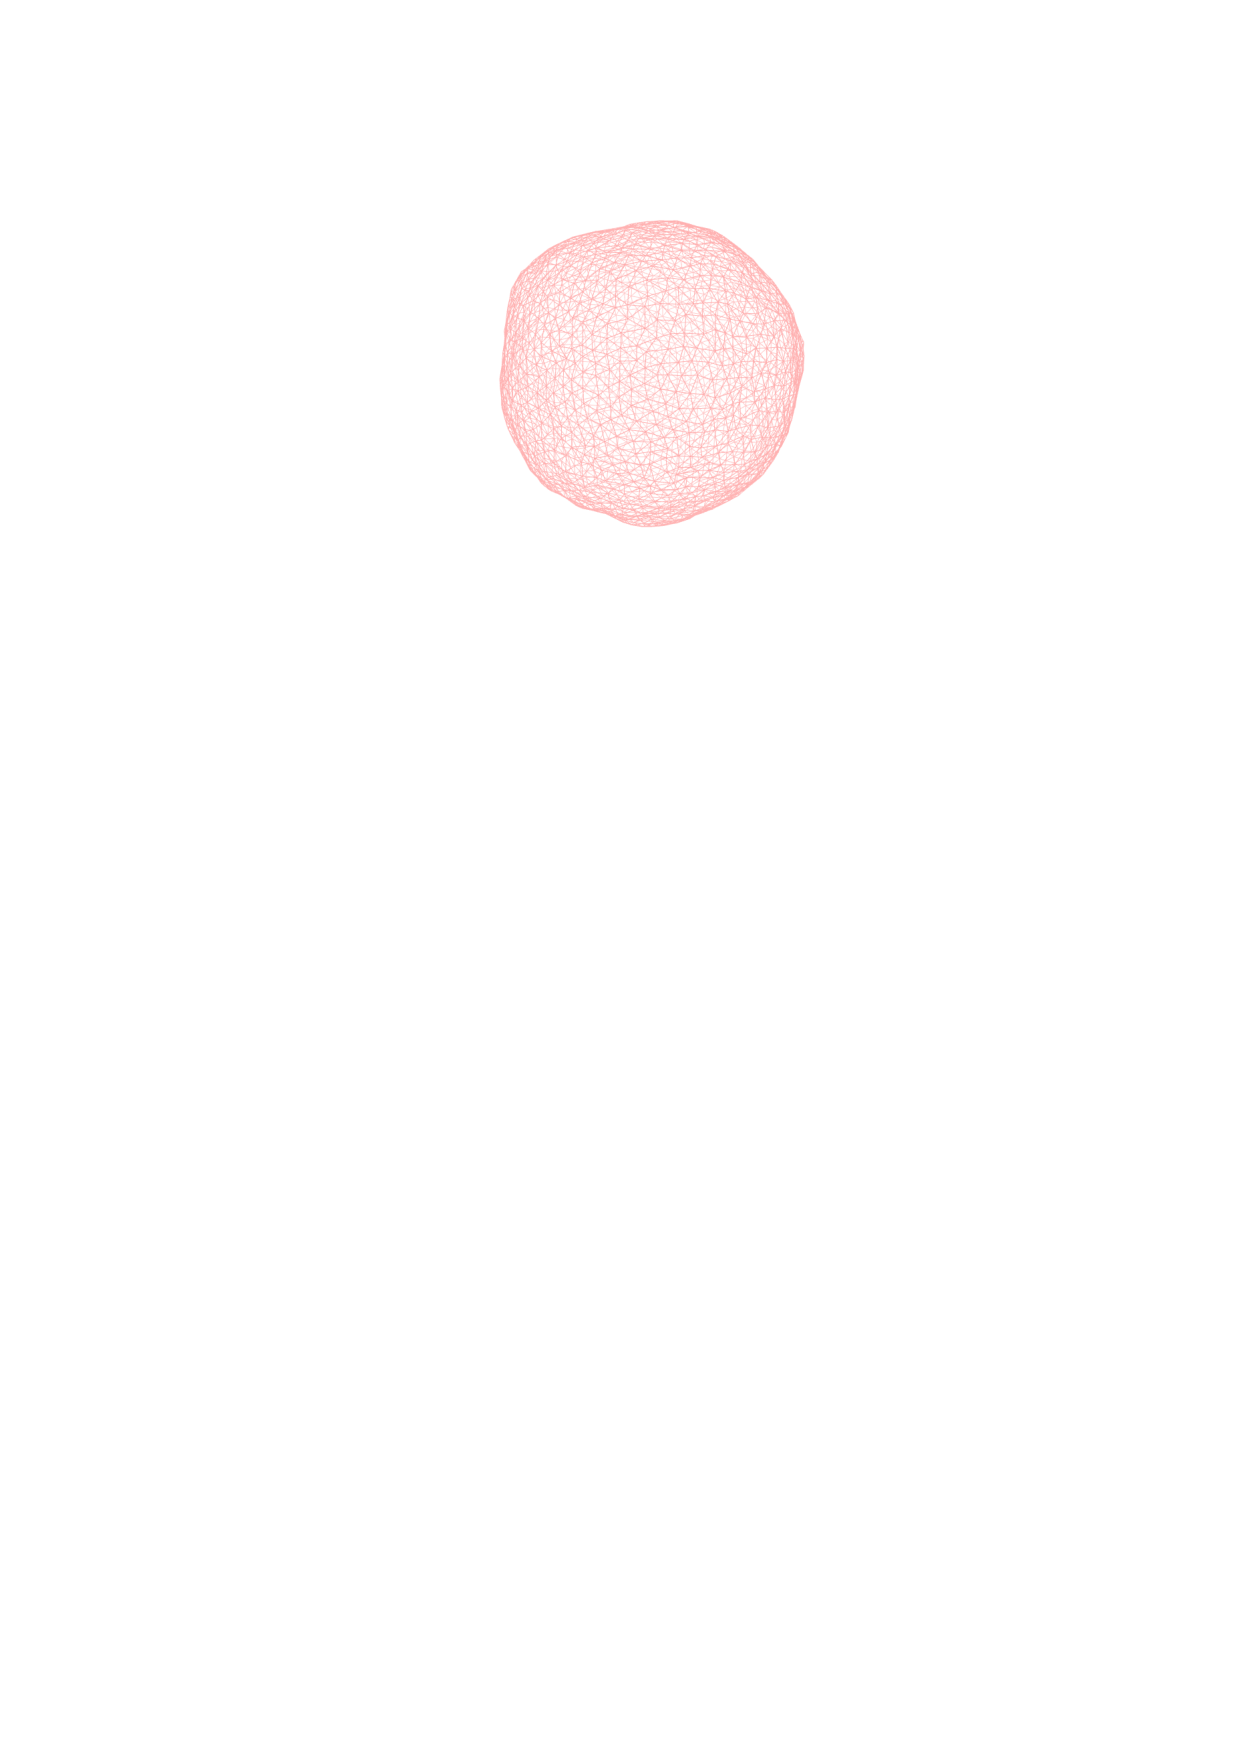
\includegraphics[width=4in]{Figs/mem_sim1}
\caption{
غشا با هندسه‌ی کروی.
}
\label{fig:mem1}
\end{center}
\end{figure}
\begin{figure}[h]
\begin{center}
\includegraphics[width=4in]{Figs/nelsonS1}
\caption{
مبدا مختصات مماس به بخشی از کره‌ی بدون تغییر شکل.ٓ
}
\label{fig:nelson_figs1}
\end{center}
\end{figure}

که در اینجا 
$z=Z()z_1,x_2)$
نقاط روی کره در حالت بدون اختلال را مشخص می‌کند. در نظریه پوسته‌ی کم عمق
\cite{nelsonJPhysFrance1987}
 فرض می‌شود که محل بررسی به اندازه‌ای کوچک است که شیب‌های 
$\partial_1Z\sim x_1/R$
و 
$\partial_2Z\sim x_2/R$
اندازه‌گیری شده نسبت به صفحه‌ی 
$(x_1,x_2)$
کوچک هستند. در نتیجه می‌توان معادله‌ی بالا رو به شکل زیر ساده کرد:
\begin{equation}
Z(x_1,x_2) \approx \frac{x_1^2+x_2^2}{2R}
\label{eq:nelsonS2}
\end{equation}
در نتیجه تمام تغییر شکل‌های پوسته از این حالت را می‌توان بر حسب جابجایی‌های عمود بر صفحه‌
 $f(x_1,x_2)$
و جابجایی های مماس بر صفحه 
$u_1(x_1,x_2)$
و
$u_2(x_1,x_2)$
که به ترتیب جابجایی در راستای محورهای 
$x_1$
و
$x_2$
را مشخص می‌کنند، تعریف کرد. بنابراین با توجه به میدان‌های تعریف شده، نقطه‌ی 
$(x_1,x_2,Z(x_1,x_2))$
در حالت بدون جابجایی در مرتبه‌ی اول به نقطه‌ی 
$(x_1+u_1-f\partial_1Z,x_2+u_2-f\partial_2Z,Z+f)$
منتقل می‌شود که در اینجا 
$\partial_iZ=x_i/R$
است. تانسور کرنش با توجه رابطه‌ی میان اندازه‌ی یک عنصر خط در حالت تغییر حالت داده شده
$ds'$
و خط متناظر آن در حالت کاملا کروی تعریف می‌شود:
\begin{equation}
(ds')^2=ds^2+2u_{ij}dx_idx_j
\label{eq:nelsonS3}
\end{equation}
در نتیجه با صرف نظر از مشتق‌های مرتبه‌های بالاتر می‌توان تانسور کرنش را تعریف کرد،
\begin{equation}
u_{ij}=\frac{1}{2}(\partial_iu_j+\partial_ju_i+\partial_if\partial_jf)-\delta_{ij}\frac{f}{R}
\label{eq:nelsonS4}
\end{equation}
در نتیجه انرژی کششی به شکل زیر تعریف خواهد شد
\begin{equation}
G_s=\frac{1}{2}\int dS\left[2\mu u_{ij}^2+\lambda u_{kk}^2\right]
\label{eq:nelsonS5}
\end{equation}
  که در اینجا 
$\lambda$
و
$\mu$
ضرایب لامه
\LTRfootnote{Lamé}
بوده و 
$dS$
عنصر مساحت است. همچنین انرژی هلفریش
\LTRfootnote{Helfrish}
را نیز در برای تغییرات خمشی پوسته در نظر می‌گیریم
\cite{Helfrich1973}.
\begin{equation}
G_b=\frac{1}{2}\int dS\left[\kappa(H-H_0)^2+\bar\kappa K\right]
\label{eq:nelsonS6}
\end{equation}
  که در اینجا 
$\kappa$
سختی خمشی، 
$H$
خمش متوسط (یا رد
\LTRfootnote{trace}
تانسور خمش)،
$H_0$
خمش ذاتی غشا،
$\bar\kappa$
مدول خمشی زینی،
و
$K$
دترمینان تانسور خمش است . با توجه به نظریه گاوس و بونه
\LTRfootnote{Gauss-Bonnet}
این انتگرال فقط یک عدد ثابت است که به انرژی آزاد سیستم اضافه می‌شود. در نتیجه از الان به بعد آن را در نظر نمی‌گیریم. همچنین فرض می‌کنیم که غشا خمش ذاتی ندارد. در نتیجه در قسمت کم عمق پوسته خمش موضعی بر حسب 
$Z(x_1,x_2)$
و 
$f(x_1,x_2)$
به شکل زیر محاسبه می‌شود:
\cite{Helfrich1973}.
\begin{equation}
H =\nabla^2(Z+f)=\frac{2}{R}+\nabla^2f
\label{eq:nelsonS7}
\end{equation}
که 
$\nabla^2=\partial_{11}+\partial_{22}$
لاپلاسین در دستگاه مختصات تعریف شده است. و در نهایت کار ناشی از فشار خارجی به صورت زیر تعریف می‌شود،
\cite{Helfrich1973}.
\begin{equation}
W=-p\int dSf
\label{eq:nelsonS8}
\end{equation}

و در نهایت  عنصر سطح به شکل زیر تعریف می‌شود،
\begin{equation}
dS=dx_1dx_2/\sqrt{1-(x_1^2+x_2^2)/R^2}\approx dx_1dx_2
\label{eq:nelsonS8.1}
\end{equation}
در نهایت با جمع کردن جملات انرژی کششی، خمشی، و فشار انرژی کشسانی سیستم به شکل زیر تغریف می‌شود:
\begin{equation}
G = G_s + G_b. + W =\int d^2x\left[\frac{\kappa}{2}(\nabla^2f)^2+\mu u_{ij}^2+\lambda u_{kk}^2-pf\right]
\label{eq:nelsonS8.2}
\end{equation}
همانطور که از نام این نظریه پیداست مدل بالا برای محاسبه‌ی انرژی لازم برای تغییر شکل‌ها کم عمق و کوچک است. مقیاس ما از اندازه‌ی کره شعاع آن
$R$
است. حد اندازه‌ی یک تغییر شکل کوچک را می‌توانیم با مقایسه‌ی انرژی کششی و خمشی محاسبه کنیم. انرژی کششی و خمشی برای قسمتی به اندازه‌ی
$\ell$
را با 
$G_s\sim Y(f/R)^2$
، که در اینجا $Y$ یک ثابت کششی‌ متداول است، و 
$G_b\sim\kappa f^2/\ell^4$
می‌توان تقریب زد. برابر قرار دادن این دو جمله، مقیاس طولی فوپل فون کارمان
\LTRfootnote{Föpplٓ-von Kármán}
را به ما می‌دهد
\begin{equation}
\ell^*=\frac{R}{\gamma^{1/4}}
\label{eq:nelsonS9}
\end{equation}
که در بالا عدد فوپل فون کارمان 
$\gamma=YR^2/\kappa$
است
\cite{nelsonPRE2003}
. با کمی محاسبه‌ی بیشتر می‌توان نشان داد که ثابت کششی که استفاده کردیم مدول ۲ بعدی یانگ است که برابر است با
\cite{nelsonPRA1988}
باید محاسبات دقیق رو از این مرجع بیارم و برای شبکه‌ی مثلث بندی با ۶ همسایه‌گی محاسبات رو بیارم.
\begin{equation}
Y= \frac{4\mu(\mu+\lambda)}{2\mu+\lambda}
\label{eq:nelsonS9.1}
\end{equation}
با فرض داشتن یک پوسته‌ی کشسان با ضخامت $h$ و جایگذاری $\kappa$ و $Y$ با مدول ۳ بعدی یانگ برای یک ماده جامد همسان کشسان در نظریه پوسته‌ی کم عمق $\gamma\approx10(R/h)^2$ بدست می‌آید 
\cite{landau}
برای اینکه این نظریه پیشبینی درستی از مسئله داشته باشد نیاز است که $\ell^*\ll R$. پس این نظریه تنها زمانی که $\gamma\gg1$ یا $r\gg h$ باشد صادق است که این حد دقیقا متناظر با پوسته‌های نازکی است که می‌توانند تحت تاثیر بسیار زیاد افت و خیز ترمودینامیکی قرار بگیرند. کویتر
\LTRfootnote{Koiter}
در مطالعاتی نیز در مورد صحت پاسخ نظریه‌ی پوسته‌های کم عمق در مقایسه با نظریه‌های عمومی‌تر که می‌توان بر تمامی یک پوسته‌ی کشسان اعمال کرد را در حالتی که از دو نقطه‌ی قطبی به یک پوسته فشار وارد می‌شود بحث کرده است
\cite{koiter1963}
 . همچنین توسط هاتچینسون
\LTRfootnote{Hutchinson}
برای مطالعه‌ی پایداری پوسته‌های تحت فشار مطالعه شده‌است
\cite{Hutchinson1967}
. در هر دو مطالعه نشان داده شده که این نظریه در مقیاسی که در بالا محاسبه کردیم رفتار درستی از سیستم را نشان می‌دهد. از آنجایی که افت و خیز گرمایی روی پوسته‌هایی که شعاع آنها بسیار بزرگ‌تر از زخامتشان است تاثیر زیادی‌ می‌گذارد، این نظریه را می‌توان به عنوان نقطه‌ شروع توصیف این سیستم‌ها استفاده کرد.
\section{
از میان رفتن مُدهای فنونی درون صفحه‌ای و انقباض هماهنگ کروی بوسیله‌ی انتگرال گاووسی
}
\LTRfootnote{Elimination of in-Plane Phonon Modes and Uniform Spherical Contrac- tion by Gaussian Integration}
یک پوسته‌ی کروی تحت فشار هماهنگ خارجی که از حد مچاله شدن کره
\LTRfootnote{buckling}
کمتر است باعث می‌شود که کره در تمام نقاط به صورت هماهنگ به اندازه‌ی $f_0$ منقبض شود. در نتیجه‌ تغییر شکل‌های خارج از صفحه‌ای را می‌توان به صورت مجموع قسمت‌های هماهنگ و غیر هماهنگ نوشت،
\begin{equation}
f(\boldsymbol x)=f_0+f'(\boldsymbol x) = f_0+\sum_{\boldsymbol . q\neq0}f_{\boldsymbol q}e^{-i\boldsymbol q.\boldsymbol x}
\label{eq:nelsonS10}
\end{equation}
در اینجا $f'(\boldsymbol x)$ 
نماینده‌ی سهم میدان از مد‌های غیر صفر مولفه‌های فوریه‌ی آن است. در این بخش برای ساده سازی از نرمال کردن 
$f_{\boldsymbol q} \equiv \frac{1}{A}\int d^2xf(\boldsymbol x) e^{i\boldsymbol q.\boldsymbol x}$
استفاده شده که $A$ مساحت انتگرال گیری شده روی صفحه‌ی $(x_1,x_2)$ است. همچنین تبدیل واروون را نیز به شکل 
$f(\boldsymbol x) = \sum_{\boldsymbol q}f_{\boldsymbol q}e^{-i\boldsymbol q.\boldsymbol x}$
در این صورت 
$\int d^2xf'(\boldsymbol x)=0$
است و در نتیجه تنها جمله‌‌ی $f_0$ در محاسبه‌ی کار فشار باقی می‌ماند. از آنجایی که جمله‌ی $f'$ تنها در قسمت غیر خطی تانسور کرنش ظاهر می‌شود، پس انرژی کشسانی که در معادله‌ی \ref{eq:nelsonS8.2} تعریف شد در حالت انقباض تحت فشار هماهنگ $f_0$ و همچنین تحت جابجایی مُدهای درون صفحه‌ای $u_1(\boldsymbol x)$ و $u_2(\boldsymbol x)$ به شکل همسان
\LTRfootnote{harmonic}
 عمل می‌کند. برای بررسی رفتارهای غیر همسان بهتر است که این میدان‌ها را تقریب بزنیم و از انرژی آزاد مؤثر تعریف کنیم.
 \begin{equation}
G_{eff}=-k_BT\ln\left\{\int\mathcal D\vec u(x_1,x_2)\int df_0e^{-G[f',f_0,u_1,u_2]/k_BT}\right\}
\label{eq:nelsonS11}
\end{equation}
برای اینکه انتگرال تابعی را در معادله‌ی بالا را برای تعداد مشخصی میدان جابجایی خارج از صفحه‌ای $f'(\boldsymbol x)$ بتوانیم انجام دهیم باید جملات $\boldsymbol q = 0$ و $\boldsymbol q \neq 0$ تانسور کرنش $u_{ij}$ 
را نیز از هم جدا کنیم،

 \begin{equation}
u_{ij}=\tilde u_{ij}^0+\sum_{\boldsymbol q \neq 0}\left[\frac{i}{2}\left(q_iu_j(\boldsymbol q)+q_ju_i(\boldsymbol(q)\right)+A_{ij}(\boldsymbol q)-\delta{ij}\frac{f_{\boldsymbol q}}{R}\right]e^{-i\boldsymbol q.\boldsymbol x}
\label{eq:nelsonS12}
\end{equation}
که در بالا 
 \begin{equation}
A_{ij}(\boldsymbol q)=\frac{1}{2A}\int d^2x\partial_if'\partial_jf'e^{i\boldsymbol q.\boldsymbol x}
\label{eq:nelsonS13}
\end{equation}
قسمت هماهنگ تانسور کرنش از اجزای زیر تشکیل شده
\begin{equation}
\begin{aligned}
&\tilde u_{11}^0=u_{11}^0+A_{11}(\boldsymbol 0)-\frac{f_0}{R}, \\
&\tilde u_{22}^0=u_{22}^0+A_{22}(\boldsymbol 0)-\frac{f_0}{R}, \\
&\tilde u_{12}^0=u_{12}^0+A_{12}(\boldsymbol 0)
\label{eq:nelsonS14}
\end{aligned}
\end{equation}
در بالا $u_{ij}^0$ جملات کرنشی هماهنگ درون صفحه‌ای مستقل از $f_0$. این محدودیت باعث می‌شود که $u_{11}^0+u_{22}^0=0$ باشد زیرا اگر تغییر شکل هم علامت در راستای $x_1$ و $x_2$ در پوسته وجود داشته باشد به این معناست که شعاع پوسته در حال تغییر کردن است که تغییرات این چنین در  جمله‌ی $f_0$ در نظر گرفته شده است. در نتیجه علاوه بر $f_0$
و $u_{12}^0$
تنها یک درجه‌ی آزادی مستقل دیگر وجود دارد که در تانسور کرنش تاثیر هماهنگ دارد و آن $\Delta u^0 = u_{11}^0-u_{22}^0$ است.
در نهایت لازم است که انتگرال تابعی در معادله \ref{eq:nelsonS11} را روی میدان‌های فنونی $u_i$ 
و ۳ درجه‌ی آزادی مستقل که سهم جملات هماهنگ در تانسور کرنش دارند، 
$f_0$، $\tilde u_{12}^0$، و$\Delta u^0$
را حساب کنیم. پس از حذف جملاتی که به صورت عدد ثابل ظاهر می‌شوند انرژی آزاد مؤثر شکل زیر را به خود می‌‌گیرد،
ٓ\begin{equation}
G_{eff}=\int d^2x\left[\frac{\kappa}{2}(\nabla^2f')^2+\frac{Y}{2}\left(\frac{1}{2}P_{ij}^T\partial_if'\partial_jf'-\frac{f'}{R}\right)\right]-A\frac{pR}{2}[A_{11}(\boldsymbol 0)+A_{22}(\boldsymbol 0)]
\label{eq:nelsonS15}
\end{equation}
که در بالا $P_{ij}^T=\delta_{ij}-\partial_i\partial_j/\nabla^2$ عملگر تصویری عرضی‌ است
\LTRfootnote{transverse projection operator}
. توجه کنید که در نتیجه‌ی انتگرال گیری، مؤلفه‌های لامه $\mu$ و $\lambda$ فقط از طریق مدول ۲ بعدی یانگ وارد می‌شوند. در آخر با جایگذاری
\begin{equation}
A_{11}(\boldsymbol 0)+A_{22}(\boldsymbol 0)=\frac{1}{2A}\int d^2x\left[ (\partial_1f')^2+(\partial_2f')^2\right] = \frac{1}{2A}\int d^2x| \nabla f'|^2
\label{eq:nelsonS16}
\end{equation}
در معادله‌‌ی \ref{eq:nelsonS15} 
انرژی آزاد مؤثر $G_{eff}$ دو بخش هماهنگ $G_0$ 
و غیر هماهنگ $G_1$
خواهد داشت،
\begin{equation}
\begin{aligned}
&G_0=\frac{1}{2}\int d^2x\left[\kappa(\nabla^2f')^2-\frac{pR}{2}|\nabla f'|^2+\frac{Y}{R^2}f'^2\right], \\
&G_1=\frac{Y}{2}\int d^2x\left[\left(\frac{1}{2}P_{ij}^T\partial_if'\partial_jf'\right)^2-\frac{f'}{R}P_{ij}^T\partial_if'\partial_jf'\right],
\label{eq:nelsonS16.1}
\end{aligned}
\end{equation}
در معادله‌ی بالا $Y=4\mu(\mu+\lambda)/(2\mu+\lambda)$ مدول یانگ در ۲ بعد است. جمله‌ی «جرم» $Y(f'/R)^2$ در تابعی انرژی هماهنگ میزان جفت شدگی بین تغییر شکل خارج از صفحه و کشیدگیی که درون صفحه ایجاد می‌شود را مشخص می‌کند. این جمله در نظریه‌ی صفحات یا غشاهای تخت ظاهر نمی‌شود. همچنین برهمکنشی با ضریب $-Y/2R$ نیز جمله‌ایست که مخصوص غشاهای خمیده‌است و به علت وجود تقارن در غشاهای تخت دیده نمی‌شود. نکته جالب راجع به این جملات این است که در آنها پارامترهای وابسته به اندازه سیستم در آنها وجود دارد. توجه داشته باشید که برای فشارهای رو به داخل $p>0$ در قسمت هماهنگ معادله شبیه کشش سطحی منفی و وابسته به شعاع رفتار می‌کند. در حد $R\rightarrow \infty$ و $p=0$ انرژی غشای تخت بدست می‌آید. از آنجایی که $f_0$ 
پس از انتگرال گیری ظاهر نمی‌شود و از این پس به جای 
$f'$ از 
$f$ 
استفاده خواهیم کرد. اگر تنها اثر جملات هماهنگ را درنظر بگیریم، نتایج بر اساس اصل همپاری برای مؤلفه‌های فوریه ناشی از گرما برای موج ۲ بعدی

\begin{equation}
\begin{aligned}
f_{\boldsymbol q} &= \int d^2xf(\boldsymbol x)e^{i\boldsymbol q.\boldsymbol x}, \\
\left\langle f_{\boldsymbol q}f_{\boldsymbol {q'}}\right\rangle_0 &= \frac{Ak_BT\delta_{\boldsymbol q, \boldsymbol{-q'}}}{\kappa q^4-\frac{pR}{2}q^2+\frac{Y}{R^2}},
\label{eq:nelsonS17}
\end{aligned}
\end{equation}
که در بالا $A$
مساحت قسمت انتگرال گیری است. 
بزرگی طول موج‌ها بلند به علت اندازه محدود کره به $q\gtrsim 1/R$
محدود می‌شوند. برخلاف غشاهای تخت که طول موج‌های بلند $q\rightarrow 0$
با اهنگ $k_BT/(\kappa q^4)$
به بینهایت میل می‌کند، در غشاهای خمیده جفت شدگی میان خمیدگی خارج از صفحه و درون صفحه، طول موج افت و خیزها با سقف مشخصه‌ی طول سیستم محدود می‌شوند، 
\begin{equation}
q^*=(\ell^*)^{-1}=\left(\frac{Y}{\kappa R^2}\right)^{1/4}\equiv\frac{\gamma^{1/4}}{R}
\label{eq:nelsonS17.1}
\end{equation}
که ما در اینجا حالت‌های $\gamma\gg1$
که در نتیجه $\ell^*\ll R$
را بررسی می‌کنیم. در حالی که $p$
به $p_c\equiv4\sqrt{\kappa Y}/R^2$
نزدیک می‌شود،. طول موج‌های $q=q^*$ 
ناپایدار شده و اندازه‌ی آنها به بی‌نهایت می‌رود. در نتیجه این حالت معادل با مچاله شدن پوسته‌ی کروی تحت فشارهای خارجی بالاتر از حد تحمل سیستم است. برای فشارهای بیشتر از $p_c$
نمی‌توانیم از این نظریه استفاده کنیم زیرا که تغییرات در شکل کره فراتر از تغییرات کم عمق خواهد بود.

معادله‌ی \ref{eq:nelsonS17}
 رفتار هماهنگ پوسته‌ی کروی را بیان می‌کند، برای بررسی رفتار ناهماهنگ پوسته نیاز است که به این معادله جمله‌های تصحیح کننده اضافه کنیم.
 \section{محاسبه‌ی سهم تک حلقه در خود انرژی}
 \begin{figure}[h]
\begin{center}
\includegraphics[width=4in]{Figs/nelsonS2}
\caption{
غشا با هندسه‌ی کروی.
}
\label{fig:nelsonS2}
\end{center}
\end{figure}

\begin{figure}[h]
\begin{center}
\includegraphics[width=4in]{Figs/nelsonS3}
\caption{
غشا با هندسه‌ی کروی.
}
\label{fig:nelsonS3}
\end{center}
\end{figure}
X
 قوانین فاینمن برای برگرفته شده از معادله‌ی \ref{eq:nelsonS15} 
 در شکل \ref{fig:nelsonS2}
 خلاصه شده است. از این پس مؤلفه‌های تبدیل فوریه به شکل
 $f_{\boldsymbol q}=\int d^2xf(\boldsymbol x)\exp(i\boldsymbol q.\boldsymbol x)$
 تعریف می‌شود. تبدیل فوریه‌ی وارون تغییر شکل‌های خارج از صفحه نیز به صورت
\begin{equation}
f(\boldsymbol x)=\frac{1}{A}\sum_{\boldsymbol q\neq 0}f_{\boldsymbol q}e^{-i\boldsymbol q.\boldsymbol x}
\label{eq:nelsonSٓ18}
\end{equation}
تعریف می‌شود و جمع روی تمام طول موج‌های مجاز است. خود انرژی ناشی از جمله‌ی ناهماهنگ ۳ نقطه‌ای و ۴ نقطه‌ای در شکل \ref{fig:nelsonS3}
الف خلاصه شده‌اند و این جملات برای توصیف غشای تخت نیز لازم هستند و به شکل 
\begin{equation}
-Y\int\frac{d^2k}{(2\pi)^2}\frac{\left[P_{ij}^Tq_iq_j\right]^2}{\kappa|\boldsymbol q + \boldsymbol k|^4-\frac{pR}{2}|\boldsymbol q + \boldsymbol k|^2+\frac{Y}{R^2}}
\label{eq:nelsonS19}
\end{equation}
 مجموع جملات خود انرژی ناشی از نمودارهای \ref{fig:nelsonS3}
 ب،

\begin{equation}
\begin{aligned}
\frac{Y^2}{R^2} &\int\frac{d^2k}{(2\pi)^2} \frac{1}{ 
\left( \kappa|\boldsymbol q + \boldsymbol k|^4 - \frac{pR}{2} |\boldsymbol q + \boldsymbol k|^2 + \frac{Y}{R^2} \right)
\left( \kappa k^4 - \frac{pR}{2}k^2 + \frac{Y}{R^2} \right) 
} \\
&\times\left\{ 
\frac{1}{2} \left[ P_{ij}^T(\boldsymbol q)k_ik_j\right]^2 + 
\left[P_{ij}^T(\boldsymbol k)q_iq_j\right]^2 + 
\left[P_{ij}^T(\boldsymbol k)q_iq_j\right] 
\left[P_{lm}^T(\boldsymbol{k+ q})q_lq_m\right] \right.\\
& \left.+ 2\left[P_{ij}^T(\boldsymbol k)q_iq_j\right]
\left[P_{lm}^T(\boldsymbol{q})k_lk_m\right]
\right\}
\label{eq:nelsonS20}
\end{aligned}
\end{equation}
وارون تابع همبستگی هماهنگ که در معادله‌ی \ref{eq:nelsonS17} مشاهده کردید فقط از جملات $q^0$، $q^2$، و $q^4$ تشکیل شده است و تصحیحات تک حلقه (که در معادلات \ref{eq:nelsonS19} و \ref{eq:nelsonS20} محاسبه شد) انجام شده به طیف جملاتی با همین توان‌ها و همچنین جملاتی با مرتبه‌ی $q^6$ نیز اضافه می‌کند. اگر  تصحیحات را تنها تا مرتبه‌ی $q^4$ نگه داریم می‌توانیم طیف را برای $q$های
کوچک تقریب بزنیم. 
\begin{equation}
Ak_BT\left\langle|f_{\boldsymbol q\rightarrow \boldsymbol 0}|^2\right\rangle^{-1} \equiv\kappa_Rq^4-\frac{p_RR}{2}q^2+\frac{Y_R}{R^2}+O(q^6)
\label{eq:nelsonS21}
\end{equation}
 که در بالا $Y_R$، $\kappa_R$، و $p_R$ به ترتیب مدول یانگ مؤثر، سختی خمش مؤثر، و فشار بی بعد. در مقیاس‌های طولی بزرگ اندازه‌گیری مشخصات کشسانی پوسته‌هایی که با گرما افت و خیز می‌کنند اطلاعاتی در مورد مشخصات مؤثر کشسانی در اختیار ما قرار می‌دهد. استفاده از این مشخصات بهتر از استفاده از مدول‌های خام $Y$، $\kappa$، و $p$
است که با تقریب دمای صفر رفتار پوسته در دما توصیف می‌کنند. با استفاده از معادلات \ref{eq:nelsonS19} و \ref{eq:nelsonS20} 
تا مرتبه‌ی $O(q^4)$
می‌توان انتگرال‌های تکانه را برای خود انرژی محاسبه کنیم،
\begin{equation}
Y_R=Y\left[1-\frac{3}{128\pi}\frac{k_BT}{\kappa}\frac{\sqrt\gamma}{(1-\eta^2)^{3/2}}\left(\eta\sqrt{1-\eta^2}+\pi-\cos^{-1}\eta\right)\right]
\label{eq:nelsonS22}
\end{equation}

\begin{equation}
\begin{aligned}
\kappa_R&=\kappa\left[1+\frac{1}{30720\pi}\frac{k_BT}{\kappa}\frac{\sqrt\gamma}{(1-\eta^2)^{7/2}}\right.\\
&\left.\left[\times\eta\sqrt{1-\eta^2}(-1699+3758\eta^2-2104\eta^4) \right.\right.\\
& \left.\left. +15(61-288\eta^2+416\eta^4-192\eta^6)(\pi-\cos^{-1}\eta)\right]\right]
\label{eq:nelsonS23}
\end{aligned}
\end{equation}

\begin{equation}
\begin{aligned}
\eta_R&=\eta+\frac{1}{1536\pi}\frac{k_BT}{\kappa}\frac{\sqrt\gamma}{(1-\eta^2)^{5/2}}\\
&\times\left[\sqrt{1-\eta^2}(64-67\eta^2)+3(21\eta-22\eta^3)(\pi-\cos^{-1}\eta)\right]
\label{eq:nelsonS24}
\end{aligned}
\end{equation} 
و در معادلات بالا فشار بی بعد $\eta=p/p_c$
تعریف کردیم. به طور مشخص زمانی که $\eta\rightarrow1$
این کمیت‌ها به بی‌نهایت میل می‌کنند. این جملات برای پایین‌ترین مرتبه فشار خارجی به شکل زیر تقریب زده می‌شوند،
 \begin{equation}
Y_R\approx Y\left[1-\frac{3}{256}\frac{k_BT}{\kappa}\sqrt\gamma\left(1+\frac{4}{\pi}\frac{p}{p_c}\right)\right]
\label{eq:nelsonS25}
\end{equation}

\begin{equation}
p_R\approx p+\frac{1}{24\pi}\frac{k_BT}{\kappa}p_c\sqrt\gamma\left(1+\frac{63\pi}{128}\frac{p}{p_c}\right)
\label{eq:nelsonS26}
\end{equation}

\begin{equation}
\kappa_R\approx \kappa\left[1+\frac{61}{4096}\frac{k_BT}{\kappa}\sqrt\gamma\left(1-\frac{1568}{915\pi}\frac{p}{p_c}\right)\right]
\label{eq:nelsonS27}
\end{equation}
برای محاسبه‌ی انتگرال‌های بالا باید از انتگرال‌های معادلات \ref{eq:nelsonS19} و \ref{eq:nelsonS20} روی تمام طول‌ موج‌های مجاز فضای فاز انتگرال بگیریم. طول‌ موج‌ها از حد پایین $k_{min}\sim1/R$ تا حد بالای طول موج‌ که با ثابت میکروسکوپیک شبکه‌ی شبکه تعیین می‌شود، است. از آنجایی که تمام انتگرال‌ها در حد بالا به حد فرابنفش همگرا می‌شوند می‌ توانیم $k\rightarrow\infty$. به علت وجود جمله‌ی «جرم» $\sim Y/R^2$ انتگرال در محدوده‌ی طول موج‌های کوچک خوش رفتار است، و در نتیجه می‌توان انتگرال را در این محدوده روی تمام فضای فاز دو بعدی انجام دهیم. اینکه انتگرال را برای محدوده‌ی پایین‌تر از فروسرخ یا $0<k<1/R$ انجام دهیم باعث ایجاد خطای از مرتبه‌ی $1/\sqrt\gamma$ می‌شود که برای پوسته‌های خیلی نازک قابل صرف نظر کردن است. 

با نگاه کردن به معادلات $\ref{eq:nelsonS25}، $\ref{eq:nelsonS26}، و \ref{eq:nelsonS27} می‌بینیم که در حد طول موج‌های بلند تغییر شکل‌های تابع مدول یانگ موثر کوچکتر، سختی خمش مؤثر بزرگتر، و کشش سطحی غیر صفر منفی است. این رفتار حتی وقتی که فشار خارجی صفر باشد نیز صادق است. وقتی $p/p_c$ بزرگ باشد، مدول یانگ و سختی خمش از تقریب دمای صفر کوچکتر می‌شوند و اندازه‌ی کشش سطحی مؤثر منفی که با $p_c$ تعیین می‌شود بسیار بزرگ می‌شود. محاسبات خطاهای مرتبه‌های بالاتر همگی نشان می‌دهند که با $p/p_c\rightarrow1$ تمام تصحیحات به بی‌نهایت میل می‌کنند. همچنین مشا‌هده می‌کنیم که تمام مشخصات مؤثر تابع دما و اندازه‌ی سیستم هستند زیرا که $\sqrt\gamma\sim R$ . با اینکه برای $k_BT\ll\kappa$ 
سهم تصحیحات ناچیز است ولی باید در نظر بگیریم که با بزرگ شدن شعاع سیستم $R\rightarrow\infty$ 
به بینهایت میل می‌کند. 


کشش سطحی ناشی از افت و خیز گرمایی و تابعیت قوی آن با فشار خارجی، همچنین تابعید ثابت کشسانی سیستم با اندازه‌ی سیستم مشخصات مختص غشاهای کروی است و در غشا‌های تخت دیده نمی‌شود. 
\section{بررسی با استفاده از هماهنگ‌های کروی}
یک پوسته‌ی کروی با شعاع $R$، سختی خمش $\kappa$ و مؤلفه‌های لامه $\mu$ و $\lambda$ 
در نظر بگیرید که تحت یک میدان مماسی $\boldsymbol u(u_x,u_y)$
و میدان جابجایی شعاعی $f$
قرار گرفته‌است. میدان $\boldsymbol u$
را مانند تمام میدان‌های خوش رفتار می‌توان مجموع یک بخش بدون چرخش
\LTRfootnote{curl free}
و بخش بدون واگرایی
\LTRfootnote{divergence free}
نوشت، $\boldsymbol u\equiv\nabla\boldsymbol\Psi+\boldsymbol v$ که تابع اسکالر $\boldsymbol\Psi$ قسمت غیرچرخش
\LTRfootnote{irrotational}
 را تولید می‌کند و $\boldsymbol v$ بخش مارپیچی
 \LTRfootnote{solenoidal}
 است. در بخش شعاعی مختصات شعاعی نود $i$ 
 در مختصات زاویه‌ای $(\theta,\phi)$ را می‌توانیم به شکل $r_i(\theta,\phi)=R_0+f(\theta,\phi)$
 نوشت و $R_0$ در اینجا شعاع متوسط کره‌ی در حال افت و خیز است.
 هنگام بسط دادن بر حسب هماهنگ‌ها کروی حقیقی به شکل
\begin{equation}
\begin{aligned}
&f(\theta,\phi)=R\sum_{l=0}^{l_M}\sum_{m=-l}^{m=l}A_{lm}Y_{lm}(\theta,\phi)\\
&\boldsymbol\Psi(\theta,\phi)=R^2\sum_{l=0}^{l_M}\sum_{m=-l}^{m=l}B_{lm}Y_l^m(\theta,\phi)
\label{eq:nelsonS28.1}
\end{aligned}
\end{equation} 

خواهند بود و انرژی کشسانی تغییر شکل آن تا مرتبه‌ی دوم تحت این میدان‌ها طبق معادله‌ی زیر خواهد بود \cite{krollPRE1993}

\begin{equation}
\begin{aligned}
G&=R^2\sum_{l,m}\left\{\left[\frac{\kappa}{2}\frac{(l+2)^2(l-1)^2}{R^2}+2K\right]A_{lm}^2-2Kl(l+1)A_{lm}B_lm\right.\\
&\left.+\frac{1}{2}l(l+1)[(K+\mu)l(l+1)-2\mu]B_{lm}^2\right\}+G_{sol}(\boldsymbol v)
\label{eq:nelsonS28}
\end{aligned}
\end{equation} 
که در اینجا $K=\mu+\lambda$
برابر مدول حجمی‌ 
\LTRfootnote{bulk modulus}
است. قسمت مارپیچی باعث انرژی در جابجایی شعاعی نشده و انرژی جداگانه با تابعیت $\boldsymbol v$ با تابعیت مربعی دارد. همچنین به معادله‌ی بالا انرژی ناشی از کشش سطحی منفی $-pR/2$ که در اثر انقباض ناشی از وجود فشار خارجی بوجود می‌آید را به صورت $G_s=-(pR/2)\Delta A$ اضافه می‌کنیم. در اینجا $\Delta A$ سطحی مضاعفی است که به علت تغییر شکل نسبت به شعاع میانگین ایجاد می‌شود. می‌توان میزان سطح مضاعف را بر حسب هماهنگ‌های کروی نوشت.
\cite{milnersafranPRA1987}
\begin{equation}
\Delta A\approx R^2\sum_{l>1,m}A_{lm}^2\left[1+\frac{l(l+1)}{2}\right]
\label{eq:nelsonS29}
\end{equation} 
همانند تقریب انرژی کشسانی پوسته‌های کم عمق اینجا نیز روی جملات مرتبه‌ی دوم $B_{lm}$ و $\boldsymbol v$ انتگرال می‌گیریم و انرژی آزاد مؤثر سیستم را بر حسب جابجایی شعاعی می‌نوسیم،
\begin{equation}
\begin{aligned}
&G_{eff}&=\frac{R^2}{2}\sum_{l>1,m}\left\{\frac{\kappa(l+2)^2(l-1)^2}{R^2}-pR\left[1+\frac{l(l+1)}{2}\right]\right.\\
&\left.+\frac{4\mu(\mu+\lambda)(l^2+l-2)}{(2\mu+\lambda)(l^2+l)-2\mu}\right\}A_{lm}^2
\label{eq:nelsonS30}
\end{aligned}
\end{equation} 
 با توجه به نظریه هم پاری انرژی،
\begin{equation}
\begin{aligned}
k_BT\left\langle|A_{lm}|^2\right\rangle_0^{-1}&=\\
&\kappa(l+2)^2(l-1)^2-pR^3\left[1+\frac{l(l+1)}{2}\right]+\frac{4\mu(\mu+\lambda)(l^2+l+2)}{(2\mu+\lambda)(l^2+l)-2\mu}R^2\\
&=\kappa(l+2)^2(l-1)^2-pR^3\left[1+\frac{l(l+1)}{2}\right]+\frac{Y}{1+\frac{Y}{2\mu(l^2+l-2)}}R^2
\label{eq:nelsonS31}
\end{aligned}
\end{equation} 
که $Y$ مدول یانگ ۲ بعدی است که قبل‌تر تعریف کردیم. حالا می‌توانیم با استفاده از پارامتر‌های وابسته به دمای مؤثر $Y_R$، $\kappa_R$، و $p_R$ به جای پارامتر‌های پایه‌ای تغییرات در افت خیز ناشی از گرما را تعریف کرد. ولی برای محاسبه‌ی آخرین جمله در معادله‌ی \ref{eq:nelsonS31} 
نیاز داریم تصحیحات گرمایی وارد بر مؤلفه‌های لامه $\mu$
و $\lambda$ 
را بدانیم. در محاسبات مربوط به نظریه‌ی پوسته‌های کم عمق این مؤلفه‌ها در محاسبات نهایی حذف شدند. در شبیه‌سازی که در مطالعه‌ی 
\cite{gomppernelson2012}
برای انرژی کشسانی گسسته‌سازی شده $\mu=3Y/8$
محاسبه شده. اگر فرض کنیم که تصحیحات گرمایی ناشی از مرتبه‌ی تک حلقه ناچیز است می‌توانیم فرض کنیم که $Y_R\approx Y$ 
است. با جایگذاری در معدله‌ی \ref{eq:nelsonS31} به همراه پارمتر‌های مؤثر دیگر به شکل نهایی زیر می‌رسیم،
\begin{equation}
\begin{aligned}
k_BT\left\langle|A_{lm}|^2\right\rangle^{-1}&\approx\\
&\kappa_R(l+2)^2(l-1)^2-p_RR^3\left[1+\frac{l(l+1)}{2}\right]+Y_RR^2\left[\frac{3(l^2+l-2)}{3(l^2+l)-2}\right]
\label{eq:nelsonS32}
\end{aligned}
\end{equation} 
حتی اگر تصحیحات گرمایی وارد بر $\mu$
و $Y$
از مرتبه‌ی $O(k_BT)$ 
باشد می‌توان اختلاف خطای اضافه شده هنگامی که فرض کردیم $\mu_R\approx3Y_R/8$
حد بالای 
$4[3(l^2+l-2)+4]$
نسبت به تغییرات ناهماهنگ دارد و در نتیجه هنگامی که $l>1$
یک مرتبه‌ی بزرگی کوچکتر خواهد بود.


%\renewcommand{\refname}{whatever}
%\bibliography{reference} 
%\bibliographystyle{IEEEtran}
%\renewcommand\refname{مراجع}


	        
	       
%\listoftables
\chapter{فصل ۱}
\setRL
\clearpage
\pagenumbering{arabic} 
\section{بررسی اجمالی پژوهش}


نقش فیزیکدانان در علوم زیستی ارائه دیدگاه‌های بدیع برای توصیف پدیده‌های زیستی‌است. به عنوان مثال مواد زیستی اغلب با مدل‌های فیزیک مواد نرم قابل توصیف هستند. $DNA$ یک پروتئین پیچیده‌ی بسیار بلند است که در مورد انسان‌ها طول آن به ۲-۳ متر می‌رسد\cite{Kauffman:1999yu}. قطر $DNA$ حدود ۱ نانومتر است\cite{WATSON:1953fr} و به کمک پروتئین‌های درون هسته بسته بندی و فشرده می‌شود که در این حالت آنرا کروموزوم\LTRfootnote{Chromosome} می‌نامیم. طول کروموزوم‌ها $0.2-20\mu m$ است و تنها هنگام تقسیم سلولی است که دارای نظم هستند و در کنار نسخه‌ی رونوشت‌شان به شکل X‌ با میکروسکوپ نوری قابل مشاهده هستند\cite{CHAFFEY:2003cr}. 

 ساختار کروماتین نقش مهمی در فرآیندهای سلولی دارد زیرا باعث می‌شود رشته‌ی بلند $DNA$ بیش از حد در هم تنیده نشود و برای ساز و کار‌هایی مانند خواندن و نوشتن ژن و ایجاد نسخه رونوشت قابل دسترس باشد\cite{PhysRevLett.120.088101, CHAFFEY:2003fv}. حیات سلول به ساختار کروموزوم وابسته است. در صورتی که هنگام تولید مثل سلول ساختار کروموزوم‌ها دچار اختلال شود باعث مرگ سلول می‌شود. 
 کروماتین‌ها در کنار یکدیگر تقریبا تمام فضای هسته را اشغال می‌کنند. در هسته‌ی سلول‌های انسان ۲۳ جفت کروموزوم وجود دارد که در مجموع ۴۶ کروموزوم در هر سلول قرار گرفته‌است.  به مجموعه‌ی $DNA$، چندین پروتئین، و $RNA$ کروماتین\LTRfootnote{Chromatin} گفته می‌شود. وظیفه‌ی اصلی کروماتین را می‌توان در موارد زیر خلاصه کرد:\\\\
۱-بسته بندی $DNA$ در فضای بسیار چگال\\
۲-مقاوم و آماده‌سازی $DNA$ برای تقسیم سلولی\\
۳-مراقبت از $DNA$ در مقابل آسیب\\
۴-تنظیم $DNA$ برای خوانده شدن ژن و عملیات مربوط به DNA\\

وظیفه‌ی اصلی بسته بندی $DNA$ در کروماتین به عهده‌ی هیستون\LTRfootnote{Histone} است\cite{Hammond:2017sp}. هیستون معمولا در سلول‌های دارای هسته دیده می‌شود.

 برای بررسی ساختار و نحوه‌ی مدیریت این ساختار توسط سلول نیاز به کمی کردن\LTRfootnote{Quantification}  خواص ساختار و دینامیک آن، همکاری فیزیکدانان را ممکن کرده‌است. فیزیکدانان سلول  را یک سیستم خارج از تعادلِ دارای حرکت\LTRfootnote{Dynamic}
می‌دانند که در آن اسکلت سلولی\LTRfootnote{Cytoskeleton} با پلیمریزه\LTRfootnote{Polymerise}(و دی‌پلیمریزه\LTRfootnote{Depolymerise}) شدن به صورت خودساماندهی‌ شده در ساختار‌های منظمی  قرار می‌گیرد که با قوانین فیزیک مواد نرم قابل توصیف است.\cite{Caballero:2015ty} اسکلت سلولی قادر به انتقال نیروهای خارجی به اعضای داخلی هسته است. به عنوان مثال مشاهده‌ شده‌است که هنگامی که سلول بر روی سطوح ناهموار قرار می‌گیرند شکل هسته تغییر می‌کند\cite{Heydari:2017cy}. برای بررسی تاثیر نیروهای خارجی بر هسته‌ی سلول اسکلت سلولی را بیشتر بررسی می‌کنیم.

\subsection{اسکلت سلولی}\label{lab:skeleton}
تمامی سلول‌های موجودات زنده اسکلت سلولی دارند. اسکلت سلولی یک شبکه پیچیده تشکیل شده از رشته‌ها یا فیلامنت‌\LTRfootnote{Filament}ها و لوله‌های نازک یا میکروتیوبول‌\LTRfootnote{Microtubule}هاست که در داخل سیتوپلاسم\LTRfootnote{Cytoplasm} از هسته تا غشای سلول توزیع شده‌است (شکل \ref{fig:wiki-cyto})\cite{hardin2014becker,PhysRevLett.120.068001}. این مجموعه اساس اسکلت سلولی است و بستر اسکلت برون سلولی را ایجاد می‌کند. این شبکه دائما در حال تغییر است و به طور عمومی از ۳ نوع پروتئین (شامل اکتین\LTRfootnote{Actin}) تشکیل شده است. در صورت نیاز سلول، این پروتئین‌ها با سرعت خیلی زیادی پلیمریزه (رشد) یا دیپلیمریزه (تخریب) می‌شوند. ویژگی اصلی اسکلت سلولی، که مورد توجه ماست، قابلیت آن در شکل دادن به سلول و عکس العمل در برابر نیرو‌ی خارجی است به خصوص نیروهایی که از طریق ماتریس برون سلولی\LTRfootnote{Extra-Celluler Matrix ($ECM$)} به سلول منتقل می‌شود\cite{PhysRevLett.120.068001}. مدل‌سازی توزیع نیرو در شبکه‌های پلیمری تصادفی تحت تنش به کمک روش‌های محاسباتی کامپیوتری امکان پذیر است\cite{Heussinger2007}. توزیع نیرو در شبکه‌های جرم و فنر مسئله‌ایست که بیش از یک قرن پیش  ماکسول\LTRfootnote{James Clarck Maxwell} به آن پرداخته است. یکی از نتایج مهم ماکسول این است که در یک شبکه گوی و فنر با افزاریش تعداد همسایه‌های به هم متصل انعطاف شبکه کمتر می‌شود\cite{doi:10.1080/14786446408643668}. در نتیجه اتصالات فیلامنت‌ها باید با چگالی مشخصی باشده تا بتواند ساختار سلول را حفظ کند.




\begin{figure}[h]
\begin{center}
\includegraphics[width=4in]{FluorescentCells}
\caption{
تصویر سلول اندوتلیال (Endothelial) زیر میکروسکوپ نشان داده شده‌است. در این عکس  ناحیه آبی هسته سلول،‌ سبز میکروتیوبول‌ها و قرمز فیلامنت‌های اکتین را نشان می‌دهد.\cite{wiki-cell}
}
\label{fig:wiki-cyto}
\end{center}
\end{figure}
اعضای شبکه اسکلت سلولی با یکدیگر و با پروتئین‌های درون سلول همیشه در حال برهم کنش هستند. موتورهای پروتئینی با انرژی شیمیایی حاصل از آب کافت\LTRfootnote{Hydrolysis} $ATP$\LTRfootnote{Adenosine triphosphate} اعضای این شبکه را تحت تنش\LTRfootnote{Stress} قرار می‌دهد. این انرژی سوخت لازم برای ۲ فرآیند غیر تعادلی اصلی در اسکلت سلولی را فرآهم می‌کند که نقش مهمی در پدیده‌هایی همچون مهاجرت سلول (و برخی باکتری \cite{Mignot853}) بازی می‌کند. پلیمریزه شدن فیلامنت‌ها و برهمکنش موتور‌های پروتئینی با آن‌ها به طور عمومی باعث انقباض اسکلت سلولی می‌شود\cite{Hawkins:2011eu}. 

نقش پلیمریزه شدن توسط اکتین، جریان‌های اکتومایوسینی\LTRfootnote{Actomyosin}، و سامانه‌های میکروتیوبول کینسین\LTRfootnote{Micriotubulekinesin} در حرکت سلول بر روی سطوح ۲ بعدی به خوبی بررسی شده‌است\cite{PhysRevLett.92.078101, refId0, PhysRevE.76.031921}. سلول برای حرکت روی سطوح ۲ بعدی، نقاط اتصال کانونی\LTRfootnote{Focal adhesion point} تشکیل می‌دهد. این نقاط تکیه‌گاه اکتین‌های در حال پلیمریزه شدن هستند که سلول را رو به جهت دلخواه هُل می‌دهند. در سمت مخالف جهت حرکت سلول انقباض اسکلت سلولی حاصل از جریان‌های اکتومایوسینی بر نقاط چسبنده‌ی کانونی غلبه می‌کند و سلول را از سطوح جدا میکند\cite{Hawkins:2011eu} (شکل\ref{fig:migration}).
\begin{figure}[htbp]
\begin{center}
\includegraphics[width=5in]{cell_sketch}
\caption{
دو فرآیند پلیمریزه‌ شدن اکتین در جلو (سمت راست) سلول در محل اتصال کانونی را نشان می‌دهد و شکسته شدن اتصالات کانونی در پشت (سمت چپ) سلول به علت انقباض ناشی از جریان اکتومایوسینی دلایل اصلی برای حرکت سلول بر روی سطوح ۲ بعدی.
}
\label{fig:migration}
\end{center}
\end{figure}


\subsubsection{انقباض و اتصال}\label{lab:traction}
نیروهای حاصل از انقباض و نیروهای منتقل شده به نقاط اتصال کانونی نقش مهمی در فرآیندهای مکانیکی سلول بازی می‌کنند. تعادل این دو نیرو شکل سلول و نحوه‌ی مهاجرت سلول بر روی سطوح ۲ و ۳ بعدی همچنین در میان سلول‌های دیگر را تعیین می‌کند. به از بین رفتن تعادل طبیعی این نیروها می‌تواند باعث تولید توده‌های سلولی و یا نفوذ سلول به داخل بافت‌های اطراف شود (مثلا تغییر اندازه‌ی هر یک از این نیروها نسبت به حالت تعادلی)  \cite{doi:10.1080/19336918.2015.1008329}.






\begin{figure}[htbp]
\begin{center}
\includegraphics[width=4in]{Epithelial}
\caption{
سلول مخاطی انتهای روده را نشان می‌دهد. اسکلت سلولی با رنگ سبز نشان داده شده است.\cite{10.1371/journal.pone.0030247}
}
\label{fig:Epithelial}
\end{center}
\end{figure}
بافت‌های مخاطی\LTRfootnote{Epithelial}(شکل \ref{fig:Epithelial}) ۶۰ درصد سلول‌های بدن انسان را تشکیل می‌دهند و معمولا بیش از ۹۰ درصد سلول‌های سرطانی از این بافت‌ها شروع می‌شود \cite{doi:10.1080/19336918.2015.1008329}.

تغییر شکل سلول‌های مخاطی و مهاجرت آنها شامل تغییرات در انقباض مکانیکی سلول است که انرژی خود را از اسکلت سلولی اکتومایوسینی تامین می‌کند. فعالیت‌های این سلول از برهمکنش‌ آن با اسکلت خارج سلول و  سلول‌های دیگر تاثیر می‌پذیرد. این سلول‌ها حرکت محدودی دارند و با سرعت کمی مهاجرت می‌کنند. این محدودیت حاصل از اتصالات قوی و قابل انبساط است که شبکه‌ی درونی و بیرونی را تثبیت می‌کند \cite{LANGE20132418}. در رشد تومورِ سلول‌های مخاطی اختلال در فرآیندهای مختلف مثل نقاط اتصال نامنظم و برهمکنش‌های مکانیکی تغییر یافته بین اسکلت درون سلولی و برون سلولی مشاهده شده‌است \cite{LANGE20132418}. در نتیجه رشد بافت تحت تاثیر ساز و کار اتصالات و برهمکنش اسکلت سلولی قرار می‌گیرد. به طور مثال شبکه برون سلولی در تومورهای مخاطی ۵-۲۰ برابر سخت‌تر نسبت به حالت عادی گزارش شده‌است \cite{Paszek:2005qq}. افزایش سختی شبکه برون سلولی ناشی از افزایش نیروهای انقباضی و تعداد نقاط اتصال کانونی است \cite{LANGE20132418}. عکس العمل این نیرو‌ها به سطوحی که سلول روی آن قرار دارد وارد می‌شود و باعث می‌شود که شکل محیط اطراف نیز تغییر کند \cite{PhysRevB.14.3438}.



\subsection{ویسکوالاستیسیته}
مجموعه‌ی اسکلت سلول پاسخ سلول و توزیع نیروی داخل سلول را مشخص می‌کند. در چند بخش  پیشرو سعی شده خصوصیت این شبکه و مدل‌های که رفتار این شبکه ‌را توصیف می‌کنند معرفی شود. برای نوشتن این بخش از منابع \cite{doi, Viscoelasticity, visco} و برای اطلاعات بیشتر توسیه می‌شود که به این منابع مراجعه فرمایید.
\subsubsection{ساز و کار مولکولی}
پلیمرْ\LTRfootnote{Polymer} مولکولی متشکل از رشته‌ی بلندی از اتم‌هاست. عکس العمل یک پلیمر به نیروی خارجی در مقیاس اتمی به دو نوعِ عمومی تقسیم می‌شود. هنگامی که پلیمر تحت تنش قرار می‌گیرد مکان و زاویه اتم‌ها  نسبت به یکدیگر تغییر می‌کند و باعث افزایش انرژی درونی‌ آن می‌شود. مقیاس زمانی این عکس العمل در حدود $\sim10^{-12}$ ثانیه است. در صورت منعطف بود پلیمر  ممکن است که دو اتم آزادی لازم برای چرخیدن نسبت به محور خط واصل‌شان را نیز داشته باشند. مثالا چرخش پلیمر حول پیوند‌ کربن-کربن تغییر زیادی در چیدمان پلیمر‌ها ایجاد می‌کند. همچنین در صورت مناسب بودن ساختار، برخی پلیمر‌ها در راستای تنش کشیده می‌شوند که باعث کاهش انتروپی\LTRfootnote{Entropy}  می‌شود. پلیمر‌های تشکیل دهنده‌ی لاستیک‌ با این فرآیند کار می‌کنند و با تغییرات خیلی کم در پیوند‌های کوالانسی‌شان انرژی درونی‌شان تغییر می‌کند. طبق قانون دوم ترمودینامیک سهم انتروپی در کار انجام شده توسط این فرآیند با دما تعیین می‌شود،
\begin{equation}
fdx=dU-TdS.\label{eq:second_thermo}
\end{equation}
معادله بالا نشان می‌دهد که با تغییر دما می‌توان نقش انتروپی در خواص الاستیکی پلیمر‌ها را مشخص کرد. نتیجه‌ی مستقیم این رابطه همچنین بیان می‌کند که نیروی لازم برای نگه‌داشتن یک نوار الاستیکی در یک طول مشخص به همراه بالا رفتن دما افزایش می‌یابد چرا که انرژی بیشتر صرف غلبه بر حرکات تصادفی پلیمر‌های تشکیل دهنده می‌شود. و در نقطه مقابل در یک میله استیل خواص انتروپی اتم‌ها سهم مهمی در خواص الاستیکی آن ندارند و انبساط دمایی نیروی الاسیتیک میله را کاهش می‌دهد.
البته عوامل فیزیکی و شیمیایی زیادی بر خواص مولکولی پلیمر‌ها تاثیر می‌گذارد، مانند ساختار مولکولی، دما، وجود محلول‌هایی که بر پلیمر اثر ‌می‌گذارند (مثالا محلول‌های که باعث تورم یا متمرکز شدن پلیمر‌ها شوند).  
\subsubsection{گرانروی، الاستیسیته،  و ویسکوالاتستیسیته}
عکس العمل مواد هوکی که تحت تنش مانند شکل \ref{fig:3.2}.الف قرار گرفته‌اند  با رابطه‌ی خطی 
\begin{figure}[htbp]
\begin{center}
\includegraphics[width=5in]{Fig3_2}
\caption{
الف) یک چیدمان آزمایشگاهی برای اندازه‌گیری خواص مکانیکی مواده را نشان می‌دهد. ماده بین دو صفحه موازی قرار گرفته و در زمان $t=0$  نیروی ثابت $F$ به صفحه بالایی اعمال شده و در زمان $t_0$ نیرو قطع شده‌. ب) پاسخ ماده شبه جامد. ج) پاسخ ماده شبه شاره.
}
\label{fig:3.2}
\end{center}
\end{figure}


\begin{equation}
\sigma=G\gamma
\label{eq:elastic}
\end{equation}
توصیف می‌شود. که در آن $\gamma$ کرنش برشی\LTRfootnote{Shear strain}، $G$ مدول برشی\LTRfootnote{Shear modulus}، و $\sigma$ تنش برشی\LTRfootnote{Shear stress} است. از طرفی عکس العمل شاره نیوتنی تحت تنش مشابه با نرخ تغییر کرنش برشی رابطه‌ی خطی دارد،
\begin{equation}
\sigma=\eta\dot\gamma,
\label{eq:visco}
\end{equation}

که در آن $\eta$ گرانروی شاره است. در مواد نرم معمولا مجموعی از هر دو عکس العمل مشاهده می‌شود که خواصیت ویسکوالاستیکی\LTRfootnote{Viscoelasticity} این مواد را توصیف می‌کند. در شکل \ref{fig:rheo} ساختار ساده‌ای از رئومترها\LTRfootnote{Rheometers} نشان داده شده که بوسیله‌ی آن رفتار ویسکوالستیک مواد مشخص می‌شود. با استفاده از این ابزارها می‌توان تنش یکنواخت و کرنش کنترل شده‌ی وابسته به زمان در ماده ایجاد کرد. البته که می‌توان پاسخ ماده تحت کرنش ثابت و تنش وابسته به زمان را نیز مورد بررسی قرار داد.
\begin{figure}[htbp]
\begin{center}
\includegraphics[width=5in]{9_1}
\caption{
ابزارهای مورد استفاده برای اندازه‌گیری خواص ویسکوالاستیکی شاره‌. الف) شاره بین تو استوانه هم محور قرار می‌گیرد. در اینجا با ثبت نگه داشتن استوانه داخلی و چرخاندن استوانه بیرونی کرنش ایجاد می‌شود. اگر فاصله دو استوانه بسیار کم  باشد می‌توان کرنش یکنواخت در ماده ایجاد کرد. نرخ کرنش با اندازهگ‌یری سرعت چرخش و تنش با اندازه‌گیری گشتاور وارد به استوانه داخلی اندازه‌گیری می‌شود. ب) در این ابزار شاره بین یک صفحه و مخروط قرار می‌گیرد. کرنش یکنواخت با چرخاندن صفحه زیرین و ثابت نگه داشتن مخروط ایجاد می‌شود. مشابه ابزار قبل تنش و نرخ کرنش به ترتیب با اندازه‌گیری گشتاور وارد بر مخروط و سرعت چرخیدن صفحه زیرین محاسبه می‌شود.
}
\label{fig:rheo}
\end{center}
\end{figure}
شکل \ref{fig:relax} پاسخ تنش ماده ویسکوالاستیک تحت کرنش پله‌ای (معادله‌ی \ref{eq:step_stress}) را نشان می‌دهد.
\begin{figure}[htbp]
\begin{center}
\includegraphics[width=6in]{9_2}
\caption{
آزمایش واحلش تنش را نشان می‌دهد. کرنش پله‌ای که در شکل الف) نشان داده شده به ماده اعمال شده و تنش ایجاد شده اندازه‌گیری می‌شود. و در شکل ب) پاسخ مواد مختلف نشان داده ‌شده‌است.
}
\label{fig:relax}
\end{center}
\end{figure}

\begin{equation}
\begin{aligned}
%\{ 
\gamma(t)=\gamma_0\Theta(t)=
  \begin{cases}
    0       & t<0\\
    \gamma_0  & t>0
  \end{cases}
%\}
\end{aligned}\label{eq:step_stress}
\end{equation}
عکس العمل ماده تابع $\gamma_0$ کرنش اولیه، و زمان خواهد بود. برای کرنش‌های کوچک می‌توان تنش را به این صورت نوشت،
\begin{equation}
\sigma(t)=\gamma_0G(t).
\end{equation}
تابع $G(t)$ مدول واحلش\LTRfootnote{Relaxationn modulus} است. شکل \ref{fig:relax} مدول واحلش مواد مختلف را به صورت کیفی رسم می‌کند. همانطور که پیش‌تر اشاره شد رابطه‌ی کرنش و تنش برای جامد الاستیکی (هوکی، نیوتنی) خطی است و تحت کرنش ثابت تنش ثابت در ماده ایجاد می‌شود. مذاب پلیمری و محلول‌های پلیمری تحت کرنش ثابت ابتدا مقوامت می‌کنند و در ماده تنش ایجاد می‌شود. از آنجایی که محلول پلیمری مقید به حفظ شکل مشخصی نیست، با گذشت زمان و جابجایی پلیمر‌های محلول تنش به صفر کاهش پیدا می‌کند. این مواد را شاره‌های ویسکوالاستیک می‌نامیم. در جامد ویسکوالاستیک همچون لاستیک، همانطور که در بخش قبل صحبت شد، پلیمرها شکل‌ خود را حفظ می‌کنند ولی تحت تنش خارجی با تغییر شکل محدود می‌توانند انرژی درونی خود را افزایش دهند. در نتیجه پس از اعمال کرنش تنش با جابجایی و تغییر شکل پلیمر‌ها کاهش می‌یابد ولی صفر نمی‌شود.
\subsubsection{گرانروی خطی}

تنش مواد ویسکوالاستیک به کرنشی که در زمان‌های گذشته اعمال شده بستگی دارد. در نتیجه رفتار مواد ویسکوالاستیک بسیار پیچیده است. در صورتی که کرنش کوچک باشد به طوری که سیستم از حالت تعادلی خیلی دور نباشد اصل برهمنهی پابرجا خواهد بود\cite{doi}. در این صورت اگر در زمان $t_1$ کرنش $\gamma_(t_1)$ به سیستم اعمال شود پ تنش $\sigma(t_1)$ و در  زمان $t_2$ کرنش $\gamma_(t_2)$ به سیستم اعمال شود پ تنش $\sigma(t_2)$ ایجاد شود بر اساس اصل برهمنهی کرنش و تنش سیستم،
\begin{equation}
\begin{aligned}
\sigma=\sigma(t_1)+\sigma(t_2) \\
\gamma=\gamma(t_1)+\gamma(t_2)
\end{aligned}
\end{equation}
خواهد بود. اگر تغییرات کرنش بسیار کوچک باشد می‌توان به کمک اصل برهمنهی نوشت،
\begin{equation}
\Delta\gamma_i=\dot\gamma+\Delta t_i
\end{equation}
در نتیجه اگر کرنش پیچیده‌ای به سیستم اعمال شود، می‌توان فرض کرد کرنش کلی مجموعه‌ای از کرنش‌هایی است که در بازه‌های زمانی کوچکی به سیستم وارد می‌شود(شکل \ref{fig:super}) و که قابل توجیه با یک مدول واحلش است، 

\begin{equation}
\gamma(t)=\sum_i\Delta\gamma_i\Theta(t-t_1)
\end{equation}
در نتیجه هر کرنش مقطعی، $\Delta\gamma_i$ در زمان $t_i$ در سیستم تنش $G(t-t_i)\Delta\gamma_i$ را در زمان $t$ ایجاد می‌کند. پس تنش در هر زمان را می‌توان بر اساس مجموع کرنش‌هایی که در گذشته به سیستم وارد شده توصیف کرد،

\begin{equation}
\sigma(t)=\sum_iG(t-t_i)\Delta\gamma_i=\sum_iG(t-t_i)\dot\gamma(t_i)\Delta t.
\end{equation}
و اگر حد بازه‌های زمانی بسیر کوچک را در نظر بگیریم،‌ $\Delta t\rightarrow0$، 
\begin{equation}
\sigma(t)=\int_{-\infty}^tdt'G(t-t')\dot\gamma(t').
\label{eq:sigma}
\end{equation}
رفتار هر ماده‌ای که با اصل برهمنهی با استفاده معادله فوق قابل توصیف باشد را ماده ویسکوالاستیک خطی می‌نامیم. از آنجایی که یک مدول واحلش رفتار سیستم را توصیف می‌کند با داشتن مدول برای یک سیستم می‌توانیم پاسخ تنش سیستم را نسبت به هر کرنشی محاسبه کنیم. به طور مثال، اگر در زمان صفر به سیستم کرنش با نرخ ثابت وارد شود، 
\begin{equation}
\sigma(t)=\int_{-\infty}^tdt'G(t-t')\dot\gamma(t')=\dot\gamma\int_{-\infty}^tdt'G(t-t')
\end{equation}
در صورتی که که در زمان بسیار طولانی این جمع مقدار محدودی شود، با توجه به معادله \ref{eq:visco}،

\begin{equation}
\eta_0=\int_{-\infty}^tdt'G(t-t').
\end{equation}
که تعریف گرانروی در مواد ویسکوالاستیک خطی‌ است.


\begin{figure}[htbp]
\begin{center}
\includegraphics[width=4in]{9_3}
\caption{
با توجه به اصل برهمنهی می‌توان هر کرنش وابسته به زمان را به صورت جمعی از کرنش‌های پله‌ای با اندازه $\Delta\gamma_i$  نشان داد که در زمان $t_i$ به ماده اعمال شده‌است.
}
\label{fig:super}
\end{center}
\end{figure}


\subsubsection{مدل‌سازی رفتار ویسکوالاستیک}

معادله‌ی \ref{eq:elastic} با یک فنر معمولی و معادله‌ی \ref{eq:visco} با دش پات\LTRfootnote{Dash pot} مدل می‌شود و رفتار کرنش برشی این دو مدل هنگامی که تنش برشی خارجی اعمال می‌شود به ترتیب در شکل \ref{fig:3.2} ب و ج با خط چین مشخص شده‌است.
\subsubsection{مدل ماکسول}
مدل ماکسول یک فنر و یک دش پات است که ماههد شکل \ref{fig:SD} به صورت سری به هم متصل شده‌است.

\begin{figure}[htbp]
\begin{center}
\includegraphics[width=4in]{spring_dashpot}
\caption{
مدل ماکسول
}
\label{fig:SD}
\end{center}
\end{figure}

حالت تعادلی این سیستم زمانیس است که تنش برشی دو قسمت با هم برابر باشد. پس،
\begin{equation}
\gamma_1=\frac{\sigma}{G}, \quad \dot\gamma_2=\frac{\sigma}{\eta}, \quad \gamma=\gamma_1+\gamma_2.
\end{equation}
با مشتق‌گیری و جایگذاری به معادله‌ی زیر می‌رسیم که معادله‌ی ماکسول است،
\begin{equation}
\sigma+\frac{\eta}{G}\dot\sigma=\eta\dot\gamma.
\label{eq:maxwell}
\end{equation}
اگر در زمان صفر تنش برشی $\sigma_0$ به سیستم وارد شود، فنر به سرعت عکس العمل نشان می‌دهد ولی دش پات نیاز به زمان بیشتری دارد که عکس العمل نشان دهد. پس در زمان صفر
\begin{equation}
\gamma_0=\frac{\sigma_0}{G}
\end{equation}
حال کافی‌ است از  معادله‌ی \ref{eq:maxwell}  انتگرال بگریم و شرایط اولیه را جایگذاری کنیم،

\begin{equation}
\dot\gamma=\frac{\sigma_0}{\eta}\rightarrow \gamma(t)=\frac{\sigma_0}{\eta}t+\gamma_0\rightarrow \gamma(t)=\sigma_0\left(\frac{1}{\eta}t+\frac{1}{G}\right).
\end{equation}
حال اگر تنش برشی خارجی را برداریم دوباره شاهد عکس العمل بلافاصله فنر خواهیم بود ولی دش پات علاقه‌ای به از دست دادن کرنش برشی ندارد. این رفتار در شکل \ref{fig:creep_maxwell} نشان داده شده‌است.

\begin{figure}[htbp]
\begin{center}
\includegraphics[width=3in]{creep_maxwell}
\caption{
رفتار کردنش در مدل ماکسول هنگامی که در زمان صفر تنش برشی وارد شود و در زمانی بعد این تنش برداشته شود.
}
\label{fig:creep_maxwell}
\end{center}
\end{figure}

\subsubsection{مدل کلوین (وُیت)}
در مدل کلوین\LTRfootnote{Kelvin} یا وُیت\LTRfootnote{Voigt} دو عنصر فنر و دش پات را به صورت موازی به هم متصل می‌کنیم (شکل \ref{fig:KV})
\begin{figure}[htbp]
\begin{center}
\includegraphics[width=4in]{kelvin_voigt}
\caption{
مدل کلوین یا وُیت را نشان می‌دهد.
}
\label{fig:KV}
\end{center}
\end{figure}
در حالت تعادلی این مدل خمش وجود ندارد در نتیجه کرنش برشی برای هر دو عنصر باید برابر باشد،
\begin{equation}
\gamma=\frac{\sigma_1}{G}, \quad \dot\gamma=\frac{\sigma_2}{\eta}, \quad \sigma=\sigma_1+\sigma_2.
\end{equation}
با یک جایگذاری ساده به معادله کلوین (وُیت) می‌رسیم،
\begin{equation}
\sigma=G\gamma+\eta\dot\gamma
\label{eq:KV}
\end{equation}
اگر در زمان صفر به این سیستم تنش برشی اعمال کنیم، فنر علاقه به افزایش طور دارد ولی دش پات نمی‌تواند تغییر طول دهد، پس تمام تنش به دش پات منتقل می‌شود و کرنش اولیه سیستم صفر است ولی با شیب اولیه‌ی $\sigma_0/\eta$ شروع می‌شود. با گذشت زمان دش پات تغییر طور می‌دهد و قسمتی و در سیستم کرنش برشی ایجاد می‌شود. در طول زمان با تغییر طول از  تنش برشی دش پات کاسته می‌شود و به تنش برشی فنر اضافه می‌شود. با گذشت زمان بسیار طولانی تنش دش پات صفر می‌شود تمام تنش را فنر تحمل می‌کند ($\sigma_0/G$).
معادله درجه اول غیر همگن \ref{eq:KV} را با شرایط اولیه توصیف شده حل می‌کنیم،
\begin{equation}
\gamma(t)=\frac{\sigma_0}{G}\left(1-e^{-\frac{t}{t_R}}\right), \quad t_R=\frac{\eta}{G}.
\end{equation}
زمان مشخصه $t_R$ زمان بازماندگی\LTRfootnote{Retardation time} سیستم است. حال اگر در زمان $\tau$ تنش را از سیستم برداریم دوباره فنر علاقه به تغییر طول دارد ولی دش پات اجازه نمی‌دهد و تمام تنش سیستم را تحمل می‌کند. حل معادله‌ی \ref{eq:KV} با کرنش صفر به شکل زیر خواهد بود،
\begin{equation}
0=G\gamma+\eta\dot\gamma \rightarrow Ce^{-\frac{t}{t_R}}.
\end{equation}
با محاسبه‌ی تنش در زمان $t=\tau$ و جایگذاری در معادله‌ی بالا،
\begin{equation}
\gamma(t)=\frac{\sigma_0}{G}e^{-\frac{t}{t_R}}\left(e^{\frac{\tau}{t_R}}-1\right), \quad t>\tau
\end{equation}
رفتار معادله‌ی فوق در شکل \ref{fig:creep_KV} نمایش داده شده‌است.
\begin{figure}[htbp]
\begin{center}
\includegraphics[width=3in]{creep_KV}
\caption{
رفتار کرنش برشی برای مدل کلوین (وُیت) را نشان می‌دهد. در زمان صفر تنش $\sigma_0$ به سیستم وارد می‌شده و در زمان $t=\tau$ بار از روی سیستم برداشته می‌شود.
}
\label{fig:creep_KV}
\end{center}
\end{figure}
\subsubsection{مدل‌های ۳ عنصری}
ترکیب دو مدل ماکسول و کلوین ساده‌ترین مدلی است که می‌تواند رفتار عمومی مواد ویسکوالستیک را توصیف کند. ۴ ترکیب ممکن مدل ۳ عنصری در شکل \ref{fig:MK} رسم شده‌است.
\begin{figure}[htbp]
\begin{center}
\includegraphics[width=4in]{MK}
\caption{
مدل‌های ۳ عنصری را نشان می‌دهد. الف) جامد استاندارد ۱، ب) جامد استاندارد ۲، ج) شاره استاندارد ۱، و د) شاره استاندارد ۲ را نشان می‌دهد.
}
\label{fig:MK}
\end{center}
\end{figure}
در دو مدل‌ شکل \ref{fig:MK} الف و ب   تنش اولیه به فنر(ها) منتقل می‌شود و در لحظه‌ی اولیه اعمال تنش شاهد تغییر طول هستیم، در نتیجه این دو مدل برای توصیف جامدهای ویسکوالاستیک مناسب هستند. از طرفی در دو چیدمان شکل\ref{fig:MK} ج و د به علت منتقل شدن بار تنش اولیه به عناصر دش پات، این مدل‌ها شاره‌های ویسکوالستیک را به خوبی توصیف می‌کنند. روابط تنش و کرنش برشی چهار مدل نشان داده شده در شکل \ref{fig:MK} به ترتیب در معادلات زیر بیان شده‌است،

\begin{equation*}
\begin{aligned}
& \text{(الف} \quad \sigma+\frac{\eta}{G_1+G_2}\dot\sigma= \frac{G_1G_2}{G_1+G_2}\gamma+\frac{\eta G_1}{G_1+G_2}\dot\gamma\\
& \text{(ب} \quad \sigma+\frac{\eta}{G_2}\dot\sigma= G_1\gamma+\frac{\eta (G_1+G_2)}{G_2}\dot\gamma\\
& \text{(ج} \quad \sigma+\frac{\eta_2}{G}\dot\sigma= (\eta_1+\eta_2)\dot\gamma+\frac{\eta_1\eta_2}{G}\ddot\gamma\\
& \text{(د} \quad \sigma+\frac{\eta_1+\eta_2}{G}\dot\sigma= \eta_1\dot\gamma+\frac{\eta_1\eta_2}{G}\ddot\gamma
\end{aligned}
\end{equation*}


\subsubsection{مدول واحلش مختلط}
یکی از روش‌های تعیین گرانروی خطی مواد محاسبه پاسخ تنش به کرنش نوسانی‌ است. فرض کنید که ابزارهای شکل \ref{fig:rheo} کرنش نوسانی زیر را در ماده ایجاد کنند،

\begin{equation}
\gamma(t)=\gamma_0\cos\omega t.
\end{equation}
با جایگذاری در معادله \ref{eq:sigma} داریم،
\begin{equation}
\begin{aligned}
\sigma(t)=-\int_{-\infty}^tdt'G(t-t')\gamma_0\omega\sin\omega t\\
	      =-\int_0^\infty dt'G(t')\gamma_0\omega\sin\omega (t-t')\\
	      =\gamma_0\left[G'(\omega)\cos\omega t-G''(\omega)\sin\omega t\right]
\end{aligned}
\end{equation}
که در معادله فوق،
\begin{equation}
G'(\omega)=\omega\int_0^\infty dt\sin\omega t G(t)
\end{equation}
\begin{equation}
G''(\omega)=\omega\int_0^\infty dt\cos\omega t G(t)
\end{equation}
در نتیجه می‌توان تبدیل فوریه $G(t)$ را با $G^*(\omega)$ نشان می‌دهیم و به این صورت تعریف می‌شود،
\begin{equation}
G^*(\omega)=i\omega\int_0^\infty dtG(t)e^{-i\omega t}
\end{equation}
به عبارتی دیگر، 

\begin{equation}
G^*(\omega)=G'(\omega)+iG''(\omega).
\label{eq:g*}
\end{equation}
و  $G*(\omega)$ را مدول مختلط می‌نامیم. در این مسئله $G'(t)$  مدول ذخیره‌ای\LTRfootnote{Storage modulus} است که پاسخ الاستیک ماده و $G''(t)$ مدول از دست رفته\LTRfootnote{Loss modulus} است که پاسخ گرانروی سیستم را نشان می‌دهد. مواد ویسکوالاستیک ترکیبی از رفتار‌ شاره و جامد را از خود نشان می‌دهند. یکی از روش‌های تعیین اینکه ماده جامد است یا شاره نگاه کردن به مدول مختلط در فرکانس‌های کوچک است. فرض کنید که مدول مختلط به شکل زیر باشد.
\begin{equation}
G(t)=G_e+Ge^{-\tau/t}
\label{eq:sa}
\end{equation}

در معادله \ref{eq:sa} $G_e$ مدول تعادلی است که برای شاره‌‌ی ویسکوالستیک صفر است (شکل \ref{fig:relax}). در نتیجه می‌توان مدول مختلط را می‌توان به شلک زیر نوشت،
\begin{equation}
\begin{aligned}
G'(\omega)=G_e+G\frac{(\omega\tau)^2}{1+(\omega\tau)^2}
G''(\omega)=G\frac{\omega\tau}{1+(\omega\tau)^2}
\label{eq:saG}
\end{aligned}
\end{equation}
برای محاسبه‌ی معالدلات \ref{eq:saG} از بست زیر استفاده شده‌است،

\begin{equation}
\begin{aligned}
\int_0^\infty dte^{-\omega t}=\lim_{s\rightarrow0}\int_0^\infty dte^{-\omega t-st}\\
=\lim_{s\rightarrow0}\frac{1}{s+i\omega}=\frac{1}{s+i\omega}
\label{eq:saG}
\end{aligned}
\end{equation}
پس برای فرکانس‌های کوچک مدول مختلط به شکل زیر خواهد بود،

\begin{equation}
\begin{aligned}
G^*(\omega)=
  \begin{cases}
    G_e       & \text{برای جامد ویسکوالاستیک}\\
    i\omega G\tau=i\omega\eta_0       & \text{برای شاره ویسکوالاستیک}
  \end{cases}
\end{aligned}
\end{equation}

\begin{figure}[htbp]
\begin{center}
\includegraphics[width=5in]{9_4}
\caption{
رفتار عمومی عناصر مدول مختلط مواد ویسکوالاستیک را برای الف)جامد ویسکوالاستیک و ب) شاره ویسکوالاستیک نشان می‌دهد.
}
\label{fig:viscoSF}
\end{center}
\end{figure}
رفتار عمومی $G'(\omega)$ و $G''(\omega)$ در شکل \ref{fig:viscoSF} نمایش داده شده است. آزمایش‌‌های متعددی مشابه این رفتار‌ها را در شبکه‌های اکتینی موجود در سلول‌های زنده را نیز تایید می‌کند.





\subsubsection{بررسی رئولوژی غشا و اکتین}\label{lab:GG}

شکل \ref{fig:gg} مدول ذخیره‌ای و از دست رفته را برای یک شبکه اکتین ۳ بعدی (شکل \ref{fig:gg}.الف) و یک غشا که با دو چگالی مختلف پروتئین متصل کننده (شکل \ref{fig:gg}.ب و شکل \ref{fig:gg}.ج) به شبکه اکتینی متصل شده‌است را  نشان می‌دهد\cite{doi:10.1021/acs.jpcb.7b11491}. ۳ رژیم مشخص در پاسخ هر یک از این  شبکه‌ها به تنش خارجی دیده می‌شود. در شکل \ref{fig:gg} در ناحیه ۱  $G'>G''$ که نشان از این است که رفتار الاستیکی شبکه در فرکانس‌های میانی غالب است. در ناحیه ۲ رفتار توانی با نمای $0.75$ مشاهده می‌شود که با رفتار تک فیلامنتی منطبق است. و در نهایت در ناحیه ۳ رفتار ماده در فرکانس‌های پایین را می‌بینیم. در ناحیه ۳ ضریب پخش فیلامنت‌ها و ساز و کارهای مولکولی هنگام تغییر فاصله و زاویه پیوند‌های کوالانسی اهمیت دارند. مشابه این ۳ رژیم در آزمایش‌های مربوط به لایه‌ی اکتین-غشایی نیز دیده می‌شود (شکل \ref{fig:gg}.ب و ج). 

در هر ۳ آزمایش دیده‌ شده‌است که در ناحیه ۱، که مربوط به فرکانس‌های میانی است، پاسخ الاستیک ($G'$) بیشترین سهم را دارد و هنگامی‌ که شبکه اکتینی به غشا متصل می‌شود (شکل \ref{fig:gg}.ب و شکل \ref{fig:gg}.ج) ضریب الاستیک افزایش می‌یابد. سختی الاستیکی شبکه‌ی پلیمری وابسته به تعداد اتصالت میان پلیمیر هاست. از آنجایی که اتصال به غشا باعث افزایش اتصالت پلیمری می‌شود اختلاف سختی بین شکل \ref{fig:gg}.ب و ج را می‌توان ناشی از افزایش چگالی پروتئین‌های متصل کننده به غشا دانست\cite{doi:10.1021/acs.jpcb.7b11491}.

در ناحیه ۳، که مربوط به فرکانس‌های پایین است، دیده‌ شده که شبکه‌های اکتینی نسبت به تنش‌های خارجی مقاومت زیادی نشان نمی‌دهند. در تنش‌های با فرکانس پایین فیلامنت‌ها زمان کافی برای حرکت و پخش\LTRfootnote{Difussion} در راستای تنش دارند و نقاط اتصال درون شبکه‌ای با این ساز و کار تغییر می‌کند (مدل خزیدن پلیمر‌ها\LTRfootnote{Reptation modul}). فضای در اختیار پلیمر‌ها برای واحلش در مدل خزیدن به طول پلیمر‌ها وابسته است و  تغییر رژیم از ۳ به  ۱ توسط این طول تعیین می‌شود. برای شکل\ref{fig:gg}الف طول متوسط واحلش $16\mu m$ اندازه‌گیری شده که با اندازه‌گیری آزمایشگاهی این نمونه همخوانی دارد \cite{doi:10.1021/acs.jpcb.7b11491}.



\begin{figure}[htbp]
\begin{center}
\includegraphics[width=6.5in]{GGprime}
\caption{
مشخصات ویسکوالاستیک وابسته به فرکانس لایه اکتین غشایی را نشان می‌دهد. در نمودارها مدول ذخیرا‌ه‌ای $G'$ با نقاط تو خالی و مدول از دست رفته $G''$ با نقاط تو پر نمایش داده شده‌است. خطوط مقطع  مربوط به برازش فیلامنت‌هایی است که برای توصیف آن تنها از یک زمان واحلش می‌توان استفاده کرد (ماکسول تک عنصری معادلات \ref{eq:g'} و \ref{eq:g''}). خطوط پیوسته مربوط به برازش شبکه‌ایست که با ۲ زمان‌های واحلش مشخص می‌شود (ماکسول دو عنصری معادلات \ref{eq:g'2} و \ref{eq:g''2}). شکل الف) شبکه اف-اکتین ۳ بعدی را نشان می‌دهد. ب) و ج) شبکه اف-اکتینی استکه بوسیله ازرین (Ezrin) به یک غشای لیپیدی متصل شده است و غلظت نقاط اتصال بین شبکه اف-اکتین و غشا در ب) ۳ مول٪ و در ج) ۵ مول٪ است.  خط سیاه ضخیم در الف) و ب) رفتار توانی با نمای $0.75$  و در ج) وابستگی در فرکانس‌های کم با نمای ۱ را مشخص می‌کند. برای مدلی که تنها یک  زمان واحلش (خط مقطع) دارد با رابطه‌ی $\tau=\eta/G_0$ محاسبه شده و برای الف) $\tau=139\pm15 s$، ب) $\tau=103\pm12 s$، و برای ج) $\tau=103\pm6 s$ بدست می‌آید. برای مدل دو زمانی (خط پیوسته) زمان واحلش ب) $\tau_2=28\pm4 s$، $\tau_1=121\pm9 s$ و برای ج) $\tau_2=33\pm6 s$، $\tau_1=131\pm16 s$ بدست می‌آید\cite{doi:10.1021/acs.jpcb.7b11491}.
}
\label{fig:gg}
\end{center}
\end{figure}


برای برازش داده‌های شکل  \ref{fig:gg} از مدلی که پلاگ\LTRfootnote{Plagge} و همکاران در سال ۲۰۱۶ پیشنهاد داده‌اند استفاده شده است. در این مدل فرض شده که طول اکتین‌ها بر اثر تنش تغییر نمی‌کند و تغییرات ناشی از تنش با یک پلیمر خطی که توسط یک شبکه‌ی  پلیمری موثر محاصره شده است مدل می‌شود. از آنجایی که مد‌های خمشی بسیار کم خرج‌تر از مد‌های کشسانی‌ پلیمر است در نظر نگرفتن این مدها مشکلی ایجاد نمی‌کند. در نتیجه  شبکه‌ی اکتینی که پلیمر را محاصر‌ه کرده‌است را می‌توان مانند یک راهرو فرض کرد که توسط پتانیسل‌های هارمونیک پلیمر را در درون خود هدایت می‌کند. از آنجایی که تنش‌های خارجی بر طول پلیمر اثر ندارد تنش‌ها به شکل پتانسیل داخل راهروی شبکه ظاهر می‌شود. از طرفی فرض می‌شود که شبکه‌ی اطراف پلیمر تنها از نقاط اتصال می‌توانند بر پلیمر تاثیر بگذارند \cite{doi:10.1063/1.5030169, PhysRevE.93.062502}. انرژی اتصال این پلیمر‌ها از مرتبه‌ی بزرگی دمای محیط است و عمر موثر آنها حدود چند ثانیه ‌است.\cite{doi:10.1021/acs.jpcb.7b11491} فرض می‌شود که فیلامنت‌ها در یک پتانسیل دوره‌ای یک بعدی قرار دارند که توسط نیروی خارجی دچار اختلال شده و این اختلال باعث می‌شود که فیلامنت در یک جهت بخصوص راحت‌تر حرکت کند \cite{PhysRevE.93.062502}. اختلاف در احتمال حرکت فیلامنت به معنی وجود اسطکاک در سیستم است که با مدل دش-پات\LTRfootnote{Dashpot module} توصیف می‌شود. پس می‌توانیم رفتار این شبکه را با فنر ماکسول توصیف کنیم. اینکه چند عنصر ماکسول نیاز داریم بستگی به اتصالات بین شبکه‌ای دارد. اینکه اتصالات حاصل در هم تنیدگی فیلامنت‌ها باشد یا بوسیله‌ی یک عامل پروتئینی محکم شده باشد.


پس می‌توانیم شبکه را به صورت مدول مختلط موثر زیر بنویسیتم،
\begin{equation}
\frac{1}{G^*}=\frac{1}{G_s}+\frac{1}{i\eta\omega},
\end{equation}
که $\eta$ اصطکاک حاصل از لغزش فیلامنت‌ها بر روی یکدیگر و اتصلات موقت حاصل این حرکت را توصیف می‌کند. $G_s$ هم مدول فیلامنت به طول $L$ است که با خم‌ شدن مدهایی با عدد موج $q_n=n\pi/L$ در آن ایجاد می‌شود،


\begin{equation}
\frac{1}{G_s}=\frac{1}{G_0}\sum_n\frac{\sin^2(q_nL/2)}{(Lq_n)^4+i\omega/\omega_0}.
\label{eq:Gs}
\end{equation}


که در معادله \ref{eq:Gs} $G_0$ مدول پلاتو\LTRfootnote{Plateau}، $\omega_0$ فرکانس جهش\LTRfootnote{Cross over} به شاخه فرکانس‌های بالاتر است. در دو حد فرکانس‌های بالا و پایین قسمت‌های حقیقی و موهموی مدول به ترتیب،
\begin{equation}
\begin{aligned}
G'_s\rightarrow G_0
  \begin{cases}
    0.38\cdot\alpha_0\cdot(\omega/\omega_0)^{3/4}       & \omega\gg\omega_0\\
    1       & \omega\ll\omega_0
  \end{cases}
\end{aligned}
\end{equation}
و
\begin{equation}
\begin{aligned}
G''_s\rightarrow G_0
  \begin{cases}
    0.92\cdot\alpha_0\cdot(\omega/\omega_0)^{3/4}       & \omega\gg\omega_0\\
    \omega/\omega_0       & \omega\ll\omega_0
  \end{cases}
\end{aligned}
\end{equation}
که می‌توان به شکل زیر نوشت،
\begin{equation}
G'_s=G_0(1+0.38\cdot\alpha_0\cdot(\omega/\omega_0)^{3/4})
\end{equation}


\begin{equation}
G''_s=G_0((\omega/\omega_0)^{-1}+(0.92\cdot\alpha_0)^{-1}\cdot(\omega/\omega_0)^{-3/4})
\end{equation}
که $\alpha_0$ حاصل جمع زدن روی تمام مدهاست و اعدادی که در دو معادله ظاهر می‌شود به علت وجود $i^{3/4}$ است،
\begin{equation}
i^{3/4}=e^{i\frac{3\pi}{8}}=\sin\frac{\pi}{8}+i\cos\frac{\pi}{8}=0.38+i0.92
\end{equation}
با جداکردن قسمت‌های حقیقی و مختلط می‌توان معادلات فوق را به شکل معادله‌ی \ref{eq:R*} بدست آورد،
\begin{equation}
G'=(\eta\omega)^2\cdot\frac{G'_s}{D}
\label{eq:g'}
\end{equation}
\begin{equation}
G''=\alpha_1\eta\omega\cdot\frac{\left((G'_s)^2+G"_s(G"_s+\eta\omega)\right)}{D}
\label{eq:g''}
\end{equation}
که در معادلات فوق،
\begin{equation}
D=(G'_s)^2+(G''_s+\eta\omega)^2
\end{equation}


در نتیجه پارامتر‌هایی که شناور هستند، $G_0$، $\omega_0$، $\eta$، $\alpha_0$، و $\alpha_1$. پارامتر $\alpha_1$ فازی است که اجازه می‌دهد که قسمت حقیقی و موهومی را نسبت به یکدیگر تنظیم کنیم. در شکل \ref{gg} خطوط گسسته با توجه به معادلات \ref{eq:g', eq:g''} فیت شده‌اند. زمان مشخصه‌ی ایجاد و فنای اتصالات بین فیلامنت‌ها با $\tau=\eta/G_0$ مشخص می‌شود. در مدل اتصال دائمی‌ فیلامنت به شبکه در نظر گرفته نشده‌است، در نتیجه، این مدل برای فرکانس‌های پایین رفتار فیلامنتی که قادر به پخش\LTRfootnote{Diffusion} است، برای فرکانس‌های میانی فیلامنت با اتصالات موقت، و در فرکانس‌های بالا رفتار تک فیلامنت را به خوبی توصیف می‌کند. در شکل \ref{fig:gg}ب و ج مشاهده می‌شود که رفتار شبکه اکتین متصل به غشا را نمی‌توان تنها با یک زمان مشخصه توضیح داد. اگر فرض کنیم که یک عنصر ماکسولی دیگر نیز به شبکه اضافه شده،
\begin{equation}
G'=G'_1+\alpha_3\cdot G'_2
\label{eq:g'2}
\end{equation}
و
\begin{equation}
G''=G''_1+\alpha_2\cdot G''_2.
\label{eq:g''2}
\end{equation}
از آنجایی که در هر دو شکل شاهد ناحیه پلاتو دوم نیستیم، انتظار می‌رود که ضریب مدول ذخیره‌ای دوم بسیار کوچکتر از مدول تلف باشد، $\alpha_3\ll\alpha_2$. نکته مهم این است که مشخص شده‌است که هنگام اتصال به غشا پ معرفی پروتئین‌های واصل، زمان مشخصه‌ی جدیدی به سیستم وارد می‌شود که مانند عنصر دوم ماکسول عمل می‌کند. برای این آزمایش بخصوص زمان مشخصه دوم که مربوط به اتصال پروتئین ازرین\LTRfootnote{Ezrin} است، $\tau=0.03 s^{-1}$ گزارش شده‌است. \cite{doi:10.1021/acs.jpcb.7b11491}

\subsection{هسته}\label{lab:nucleus}

\subsubsection{نقشه برداری از برهمکنش‌های کروماتین‌ها}
نحوه‌ی تا شدن کروموزم‌ها داخل هسته اطلاعات زیادی در مورد ساختار کروموزوم در اختیار ما قرار می‌دهد. این اطلاعات می‌تواند نشانه‌ی از سازوکار فعالیت ژن‌ها\LTRfootnote{أGene Activity} و به طور کلی وضعیت هسته در اختیار ما قرار دهد. با روش های-سی\LTRfootnote{Hi-C} \cite{Lieberman-Aiden289} می‌توان برهمکنش ژن‌ها را در داخل هسته دنبال کرد. به طور خلاصه در این روش قسمت‌های مختلف کروماتین  علامت گذاری می‌شود.  ماتیریسی شکل \ref{fig:Hi-C} یکی از نتایج این آزمایش را نشان می‌دهد. رشته‌ی کروموزوم به مناطق یک میلیون جفت بازی\LTRfootnote{Mega Basepare} ($1MB$)  تقسیم می شود که به آن لوکس\LTRfootnote{Locus} گفته می‌شود. هر عضو ماتریس $M$، $m_{ij}$  تعداد اتصالات بین لوکی\LTRfootnote{Loci} (جمع لوکس) $i$ و $j$ را مشخص می‌کند.
\begin{figure}[htbp]
\begin{center}
\includegraphics[width=3.5in]{Hi_C}
\caption{
  قسمتی از ماتریس اتصال مربوط به کروموزم ۱۴ را نشان می‌دهد. هر پیکسل وضعیت اتصال یک لوکس $۱MB$ با یک لوکس $1MB$ دیگر را نشان می‌دهد. شدت رنگ مشخص کننده تعداد اتصالات بین دو لوکس است. خطوط روی محورها به فواصل $۱۰MB$ رسم شده‌است \cite{Lieberman-Aiden289}.
}
\label{fig:Hi-C}
\end{center}
\end{figure}



مطالعه ماتریس اتصال نشان می‌دهد که در طول کروموزم نواحی متشکل از لوکی‌های زیادی وجود دارد که یا علاقه به ایجاد اتصال زیاد با نواحی دیگر دارند یا اتصالات کمتری ایجاد می‌کنند. این نواحی  به طور عمومی‌ با دو دسته لوکی تقسیم بندی می‌شود، لوکی $A$ دارای نواحی با اتصالات کم و لوکی $B$ با اتصالات زیاد است. وجود اتصالات زیاد در ناحیه $B$ خبر از این می‌دهد که در این ناحیه کروموزم بیشتر پَک\LTRfootnote{Pack}  شده‌است. به عبارت دیگر ژن‌هایی که در نواحی نوع $B$ قرار دارد علاقه‌ی بیشتری به چیدمان‌های فضایی نزدیک به هم دارند. همچنین نتایج آزمایش‌ فیش سه بعدی\LTRfootnote{3D-FISH} نیز تایید می‌کند که قسمت‌هایی از کروماتین که در نواحی مشابه قرار دارند ($A$ یا $B$) در نزدیکی یکدیگر ظاهر می‌شوند. 
\begin{figure}[htbp]
\begin{center}
\includegraphics[width=4.5in]{chromatin_coarse_grained}
\caption{
 معماری کروماتین را در ۳ مقیاس مختلف نشان می‌دهد. در شکل بالا کروموزوم‌ها را نشان می‌دهد که هر کدام در فضا‌های جدا و مشخص قرار دارند. در شکل وسط نواحی باز و بسته را نشان می‌دهد که رشته‌ی کروماتین از میان این نواحی می‌گذرد. و در شکل پایین رفتار کروماتین را در مقیاس یک میلیون جفت بازی می‌بینیم که به صورت گلبول فرکتالی رفتار می‌کند \cite{Lieberman-Aiden289}.
}
\label{fig:chromo_coarse}
\end{center}
\end{figure}

\subsubsection{ساز و کار کروماتین در هسته }
در حال حاضر تصور ما از کروموزوم‌های داخل هسته‌ی سلول‌ها آرایشی به دور از رشته‌های در هم تنیده‌ی نامنظم است \cite{Gibcus:2013fj,Lieberman-Aiden289}. در این بخش علاقه داریم که نظم این سیستم در هم‌تنیده‌ و پیچیده‌ را در مقیاس بزرگ یعنی در مقیاس میلیون جفت بازی\LTRfootnote{Mega Basepare} مطالعه کنیم. یکی از مدل‌ها درشت دانه برای توصیف رفتار گزارش شده توسط آزمایش های-سی  مدل درشت‌ دانه‌ی پیشنهاد شده توسط \cite{Lieberman-Aiden289} است که در شکل \ref{fig:chromo_coarse} نشان داده شده‌است. در این مدل کروماتین رشته‌ی بلندی درون هسته در نظر گرفته می‌شود که از دو عنصر $A$ و $B$ تشکیل شده‌است.   در این مقیاس کروماتین در فضاهای مشخصی قرار دارد\cite{Gibcus:2013fj,Lieberman-Aiden289}. همچنین نتایج اندازه‌گیری با روش‌های های-سی و تصویر برداری از لوکی‌ها تایید می‌کند که نواحی هم نوع ($A$ و $B$) علاقه دارند که با یکدیگر برهمکنش داشته باشند. در مقیاس پیشنهاد شده  ساز و کار فشرده شدن کروماتین وجود پروتئین‌هایی شبیه به کوهسین\LTRfootnote{Cohesin} است که که به شکل حلقه بوده و می‌توانند روی DNA حرکت کنند و طی فرآیندی حلقه‌ ایجاد کنند\cite{Nuebler196261}. شکل \ref{fig:TADloops} این مدل را نشان می‌دهد.

\begin{figure}[htbp]
\begin{center}
\includegraphics[width=5.5in]{TAD_loops}
\caption{
ردیف اول مدل ایجاد حلقه و ردیف پایین مدل جدا شدن ناحیه‌ها در طول کروماتین را مشخص می‌کند. الف) شکل کارتونی  الگو ایجاد شده توسط مدل ایجاد حلقه‌ را نشان می‌دهد. این الگو به شکل مربع‌های نشان دهنده نواحی با احتمال اتصال بالا در راستای قطر نقشه‌ ظاهر می‌شود. از طرفی مدل تقسیم بندی فضایی کروماتین به نواحی $A$ و $B$ الگویی شطرنجی دارد. نقشه‌ی مدل ایجاد حلقه بر روی کروماتین را نشان می‌دهد. این پروتئین‌ها با مصرف $ATP$ قادر به ایجاد حلقه در $DNA$ هستند. ب) نشان می‌دهد که در حضور فاکتورهای ایجاد کننده‌ی حلقه الگوی حلقه‌ها  و در عدم حضور حلقه‌ها الگوهای شطرنجی خواهیم داشت. ج) قسمتی از شبیه‌سازی به طوب ۱۰ میلیون جفت بازی را برای هر مدل نشان می‌دهد.
}
\label{fig:TADloops}
\end{center}
\end{figure}

فرآیند ایجاد نواحی مجزای $A$ و $B$ در طول کروماتین با مدل حلقه قابل توضیح نیست. همانطور که در شکل \ref{fig:TADloops} ردیف پایین مشاهده می‌کنید، الگوی ایجاد شده توسط اتصالات لوکی‌ها در کروموزوم الگوی صفحه شطرنجی تشکیل می‌دهد. این الگو نشان می‌دهد که بخش‌هایی بر روی کروماتین با بخش‌های دیگری احتمال اتصال زیاد و با بخش‌هایی دیگر احتمال اتصال کمی دارند. از آنجایی که توزیع بخش‌های اتصال زیاد همیشه در همسایگی نزدیک آنها قرار \textbf{ندارد} الگوی شطرنجی پدید می‌آید. اما زمانی که اتصال با فرآیند ایجاد حلقه در کروماتین ایجاد ‌شود اتصالات بسیار موضعی‌است در نتیجه الگوی مربع شکل در امتداد قطر ماتریس اتصال ایجاد می‌شود (شکل\ref{fig:TADloops} ردیف بالا).
 
 یکی از مدل‌های محبوب پیشنهادِ وجود برهمکنش‌های مشخص بین نواحی است که بر اثر جدا سازی فازی قسمت‌های هم نوع در فضاهای مشخص در کنار یکدیگر قرار می‌گیرند \cite{Nuebler196261}. این نواحی با رشته‌های پلیمری مدل می‌شوند که بر روی‌ آن قسمت بندی‌های زیادی از ۲ نوع ناحیه ایجاد شده است و هر لوکی می‌تواند نوع $A$ یا $B$ باشد. این دو نوع ناحیه از لحاظ اندازه و خواص الاستیکی با یکدیگر مشابه‌اند ولی به لحاظ برهمکنش متفاوت هستند.  یعنی برای برهمکنشهای $A-A$، $B-B$، و $A-B$ انرژی مختلفی تعریف می‌شود. برای جدا سازی مناطق با محاسبه انرژی برهم کنش‌ها به هر منطقه برچسب کلی $A$ یا $B$ داده می‌شود. همچنین بین لوکی‌ها نیروی دافعه وجود دارد تا لوکی‌ها در داخل یکدیگر فرو نروند.
شبیه‌سازی همچنین نشان می‌دهد که افزایش تعداد عناصر ایجاد حلقه در کروماتین‌ها با ایجاد ناحیه‌های $A$ و $B$ مخالفت می‌کند \cite{Nuebler196261}.
نتیجه‌ی جدایی مناطق کروماتینی به دو ناحیه به وسیله مدل جدا سازی فازی با انرژی برهمکنش لوکی‌ها قایل تنظیم است. یعنی با نسبت‌های مختلف انرژی مناطق $B$ ممکن است در مرکز هسته  متمرکز شوند یا نزدیک به غشای هسته. از طرفی در اکثر سلول‌ها مشاهده شده است که کروماتین با غشای هسته اتصالات قوی برقرار می‌کنند و به دیواره‌ی هسته متصل می‌شوند. در نتیجه‌ برای مدل‌سازی این فرآیند پیشنهاد می‌شود که در انتهای هر کروماتین نواحی $B$ قرار دهیم (این پروتئین‌ها بیشتر مسئول اتصال به غشای هسته هستند) ولی برهمکنش با هسته نیز برای آن تعریف شود  \cite{Nuebler196261}.






%\section{
%اهمیت  پژوهش
%}

\clearpage
\section{طرح پژوهش}
\subsection{بخش اول}

بخشی از این پژوهش به توسعه و تکمیل مدل سلول مجازی\LTRfootnote{The Virtual Cell} می‌پردازد. این مدل مجموعه‌ای از مدل‌های شناخته شده و تایید شده‌ی فیزیکی است که رفتار مکانیکی اجزای مختلف سلول را توصیف می‌کند. این مدل ابزار اصلی برای پیش‌برد شبیه‌سازی این پژوهش خواهد بود. این مدل از بخش‌هایی همچون اسکلت برون سلولی، غشا، شبکه‌ی اکتینی، غشای هسته، و کروماتین‌های داخل آن تشکیل شده‌است. هر یک از بخش‌‌های نامرده نیاز به تنظیم و توسعه دارند تا این پژوهش را عملی سازند. برای مثال در راستای بررسی تاثیر هندسه و نیروی خارجی بر شکل هسته‌ی سلول و چیدمان کروماتین‌های درون آن، فرآیند انتقال و توزیع نیرو در مدل سلول مجازی توسعه پیدا خواهد کرد. \\


رفتار سلول نسبت به نیروی خارجی و هندسه‌ی محیط اطراف به عوامل مختلف زیستی، شیمیایی، و فیزیکی وابسته است. در شبیه‌سازی با مدل مجازی سلول می‌توانیم سهم فیریک مسائل را از بخش‌های دیگر جدا کنیم. به طور مثال اگر سلولی بر روی یک سطح مشخصی شروع به حرکت کند، با این مدل می‌توان فهمید که چه مقدار از این حرکت سهم کمینه‌سازی انرژی مکانیکی سلول است. \\


همچنین می‌توان به همکاری جدید بین گروه‌ ماده‌چگال نرم دکتر اجتهادی و گروه انبرک نوری دکتر سید ریحانی اشاره کرد. در این قسمت با استفاده از نتایج رئومتری گروه دکتر سید ریحانی بر روی گلبول‌های قرمز می‌توانیم مدل سلول مجازی را تصحیح و کالیبره کنیم. (اطلاعات بیشتر در بخش \ref{lab:GG})
\subsection{بخش دوم}
کروماتین حامل اطلاعات موجودات زنده‌است. از طرفی این اطلاعات به علت محدودیت فضای داخل سلول همیشه در دسترس نیستند. ساختار و چیدمان کروماتین درون سلول سهم مهمی در نحوه و شانس خوانده شدن ژن‌های بر روی آن دارد . افراد در سال‌های اخیر فناوری لازم برای مطالعه‌ی آزمایشگاهی این چیدمان را تهیه کرده‌اند (اطلاعات بیشتر در بخش \ref{lab:nucleus}). \\

در بخش دوم پژوهش از مدل تکمیل شده‌ی سلول مجازی برای بررسی هندسه‌ی اتصالات کروماتین (ماتریس اتصالات) و ساختار کروماتین‌ها در هسته‌ی سلول استفاده خواهد شد. در این پژوهش علاوه بر بررسی ساختار کروماتین‌ در حالت تعادلی سلول، با اعمال تنش به هسته‌ی سلول قادر به  بررسی پاسخ ساختار کروماتین و ماتریس اتصالات آن تحت نیرو‌های خارجی نیز هستیم.

\subsubsection{بخش تکمیلی}
مهاجرت سلول مسئله روز و جال دیگری است که در صورت مناسب بودن شرایط می‌ةوان در ادامه این پژوهش دنبال کرد. مهاجرت سلول فرآیندی غیر تعادلی است که بخش زیستی و فیزیکی آن هسته‌ی سلول را تحت تنش قرار می‌دهد و از حالت کره به بیضی تغییر می‌دهد. در صورت امکان می‌توان مدل‌های مهاجرت سلولی را در مدل سلول مجازی توسعه داد و تغییرات ساختار کروماتین و ماتریس اتصلات آن را تحت تنش‌های ناشی از فرآیند غیر تعادلی حرکت سلول نیز بررسی کرد (اطلاعات بیشتر در بخش‌های \ref{lab:skeleton}و \ref{lab:traction}  ).
%\section{برنامه پژوهشی}

text\cite{Dekker:2017rt}\cite{Tee:2015gf}\cite{Gerlitz:2011bh}\cite{Shi:2018uo}\cite{10.3389/fnins.2017.00559}\cite{Shaebani:2017xy}\cite{C6RA23012A}

\clearpage
\section{منابع}

\unsetRL
%\renewcommand{\refname}{whatever}
\bibliography{reference} 
\bibliographystyle{IEEEtran}
%\renewcommand\refname{مراجع}


	        
	       
%\clearpage
%\chapter{
%مدل‌سازی غشا، مدل‌های پیوسته و گسسته
%}




\unsetRL
\bibliography{reference} 

\bibliographystyle{IEEEtran}
%\renewcommand{\contentsname}{whatever}
%\renewcommand{\refname}{whatever}
%\renewcommand\refname{مراجع}

%\printbibliography[title={Reference}]

\end{document}